%%%%%%%%%%%%%%%%%%%%%%%%%%%%%%%%%%%%%%%%%%%%%%%%%%%%%%%%%%
%%  Kelvin Titimbo                                      %%
%%  Institute of Theoretical Physics                    %%
%%  Chinese Academy of Sciences                         %%
%%  November, 2020                                      %%
%%%%%%%%%%%%%%%%%%%%%%%%%%%%%%%%%%%%%%%%%%%%%%%%%%%%%%%%%%
\documentclass[a4paper,12pt,twoside]{postdoc_temp}
%\usepackage[utf8]{inputenc}
\usepackage[left=4cm,top=4cm,right=3cm,bottom=3cm]{geometry}
\usepackage{amsfonts,amsmath,amssymb,amsthm,mathrsfs}
\usepackage[scr=boondox]{mathalfa}
\RequirePackage[pdfa,bookmarksnumbered=true, pdfstartview=FitH, pdfpagelayout=OneColumn,pdftex,pdfauthor={FULL NAME},pdftitle={TITLE},pdfsubject={PostDoctoral Report ITP-CAS - December, 2020},pdfkeywords={KEYWORDS},pdfproducer={postdoc_temp},pdfcreator={Kelvin Titimbo and Kevin Hernandez},colorlinks = true,linkcolor = blue]{hyperref}

\usepackage{graphicx}
\usepackage{siunitx}
\usepackage{lipsum}
\usepackage{multirow,tabularx}
\usepackage[font=small,labelfont=bf]{caption}
\usepackage{float,subcaption}
\usepackage{cite,notoccite}
\usepackage{indentfirst}
\usepackage{xspace}
\usepackage{array}

\graphicspath{{./figures/}}

\usepackage{titlesec}
\makeatletter
\titleformat{\chapter}[frame]{\large}{\filright\enspace \@chapapp~\thechapter\enspace}{10pt}{\LARGE\bfseries\filcenter}
\titlespacing*{\chapter}{0pt}{-10pt}{50pt}
\makeatother

\fancypagestyle{biblio}{
  \renewcommand{\headrulewidth}{0.5pt}
  \setlength{\headheight}{14.5pt}
  \if@openright\cleardoublepage\else\clearpage\fi
  \fancyhead[el,or]{\thepage}
  \fancyhead[er,ol]{Bibliography}}
  
\fancypagestyle{ending}{
  \renewcommand{\headrulewidth}{0.5pt}
  \setlength{\headheight}{14.5pt}
  \if@openright\cleardoublepage\else\clearpage\fi
  \fancyhead[el,or]{\thepage}
  \fancyhead[er,ol]{\chapterhdrname}}
  

%%%%%%%%%%% FRONT PAGES %%%%%%%%%%%%%%%%%%%%%%%%%%%%%%%%%%%%%
\author{Ram Krishna Sharma}
\title{Post doctoral research report}
\instZH{\zhs{中国科学院高能物理研究所}} %Institute of Theoretical Physics
\supervZH{Prof. Mingshui Chen \zhs{陈明水}}
\dateZH{\zhs{\number\year~年 \number\month~月}} % Current date year - month
\datese{\zhs{2019 年 12 月 -- 2022 年 06 月}} % Starting date (yyyy/mm) and ending date
\psectZH{\zhs{物理学}} % Primary Scientific Sector
\ssectZH{\zhs{粒子物理与原子核物理}} % Secondary scientific sector
\nclass{}
\nsecret{}
\udc{}
\nschem{}

%%%%%%%%%%%%%%%%%%%%%%%%%%%%%%%%%%%%%%%%%%%%%%%%%%%%%%%%%%%
%%%%%%%%%%%%%%%%%%%%%%%%%%%%%%%%%%%%%%%%%%%%%%%%%%%%%%%%%%%

\providecommand{\cmsTable}[1]{\resizebox{\textwidth}{!}{#1}}

%%%%%%%%%%%%%%%%%%%%%%%%%%%%%%%%%%%%%%%%%%%%%%%%%%%%%%%%%%%
%%%%%%%%%%%%%%%%%%%%%%%%%%%%%%%%%%%%%%%%%%%%%%%%%%%%%%%%%%%

% CMS definitions
\usepackage{ptdr-definitions}
\usepackage{topcapt}% for captions at top, i.e., tables

\begin{document}
\maketitle
\preambulo
\begin{resumen}

% \noindent \lipsum[1-3].
This report summarises the work done by Ram Krishna Sharma in the CMS group of the Institute of High Energy Physics, with Prof. Mingshui Chen, from December 2019 to June 2022. The main focus was on the double Higgs non-resonant production with fully Hadronic final state of WW$\gamma \gamma$, Higgs to 4 lepton differentical and fiducial cross-section measurement and vector boson scattering measurement with semi-leptonic WW final state. Other secondary project includes the studies with CPPF, EGamma HLT studies.

\vspace*{2em}

\noindent \textbf{Keywords:} {VBS, HH, differential and fiducial measurement}
\end{resumen}







\tableofcontents
\listoffigures
\listoftables

\cuerpo
\setlength{\parskip}{0.75em}
\chapter{Introduction}
Introduction chapter..
% \lipsum[1-20]
\section{The CMS detector}\label{section:CMS_Detector}

A detailed description of the CMS detector, together with a definition of the coordinate system used and the relevant
kinematic variables, can be found in Ref.~\cite{Chatrchyan:2008zzk}.

The central feature of the CMS apparatus is a superconducting solenoid of 6 \unit{m} internal diameter, providing a
magnetic field of 3.8 \unit{T}. Within the solenoid volume are a silicon pixel and strip tracker, a lead tungstate
crystal electromagnetic calorimeter (ECAL), and a brass and scintillator hadron calorimeter (HCAL), each composed of a
barrel and two endcap sections. Forward calorimeters extend the pseudorapidity coverage provided by the barrel and
endcap detectors. Muons are measured in gaseous detectors embedded in the steel flux-return yoke outside the solenoid.
The particle-flow algorithm~\cite{CMS-PRF-14-001} reconstructs and identifies each individual particle in an event, with
an optimized combination of information from the various elements of the CMS detector.  The energy of photons is
obtained from the ECAL measurement.  The energy of electrons is determined from a combination of the electron momentum
at the primary interaction vertex as measured by the tracker, the energy of the corresponding ECAL cluster, and the
energy sum of all bremsstrahlung photons spatially compatible with originating from the electron track.  The energy of
muons is obtained from the curvature of the corresponding track.  The energy of charged hadrons is determined from a
combination of their momentum measured in the tracker and the matching ECAL and HCAL energy deposits, corrected for the
response function of the calorimeters to hadronic showers.  Finally, the energy of neutral hadrons is obtained from the
corresponding corrected ECAL and HCAL energies.

Events of interest are selected using a two-tiered trigger system.  The first level, composed of custom hardware
processors, uses information from the calorimeters and muon detectors to select events at a rate of up to 100\unit{kHz}
within a fixed latency of about 4\mus~\cite{Sirunyan:2020zal}.  The second level, known as the high-level trigger,
consists of a farm of processors running a version of the full event reconstruction software optimized for fast
processing, and reduces the event rate to around 1\unit{kHz} before data storage~\cite{Khachatryan:2016bia}.


% All of the answers are here: https://twiki.cern.ch/twiki/bin/viewauth/CMS/Internal/PubDetector

% \chapter{The CMS detector} \label{section:CMS_Detector}



% Events of interest are selected using a two-tiered trigger system. The first level (L1), composed of custom hardware processors, uses information from the 
% calorimeters and muon detectors to select events at a rate of around 100\unit{kHz} within a fixed latency of about 4\mus~\cite{CMS:2020cmk}. The second level, 
% known as the high-level trigger (HLT), consists of a farm of processors running a version of the full event reconstruction software optimized for fast processing, 
% and reduces the event rate to around 1\unit{kHz} before data storage~\cite{CMS:2016ngn}.

% for now just including a bit on photons since they are the most key object in the analysis since their invariant mass defines our signal region - maybe consider adding 
% additional object info since this analysis uses many objects. 

The electromagnetic calorimeter consists of 75\,848 lead tungstate crystals, which provide coverage in pseudorapidity $\abs{\eta} < 1.48 $ in a barrel region (EB) 
and $1.48 < \abs{\eta} < 3.0$ in two endcap regions (EE). Preshower detectors consisting of two planes of silicon sensors interleaved with a total of $3 X_0$ of 
lead are located in front of each EE detector.

In the barrel section of the ECAL, an energy resolution of about 1\% is achieved for unconverted or late-converting photons in the tens of GeV energy range. 
The energy resolution of the remaining barrel photons is about 1.3\% up to $\abs{\eta} = 1$, changing to about 2.5\% at $\abs{\eta} = 1.4$. In the endcaps, 
the energy resolution is about 2.5\% for unconverted or late-converting photons, and between 3 and 4\% for the other ones~\cite{CMS:2015myp}.

The diphoton mass resolution, as measured in \Htogg decays, is typically in the 1--2\% range, depending on the measurement of the photon 
energies in the ECAL and the topology of the photons in the event~\cite{CMS:2020xrn}.

The integrated luminosities for the 2016, 2017, and 2018 data-taking years have 1.2--2.5\% individual uncertainties~\cite{CMS-LUM-17-003,CMS-PAS-LUM-17-004,CMS-PAS-LUM-18-002}, 
while the overall uncertainty for the 2016--2018 period is 1.6\%.
\chapter{VBS production}
\section{Introduction}\label{section:introduction_VBS}

The discovery of the Higgs boson~\cite{Aad:2012tfa,Chatrchyan:2012ufa} completed the observation of the
particle content of the standard model (SM) of fundamental interactions, but the investigation of its scalar and Yukawa
sectors is still in its infancy with respect to the vast scientific program foreseen with the data that is being
delivered by the Large Hadron Collider (LHC) at CERN.

Vector boson scattering (VBS) plays a special role, since the violation of its unitarity coming from direct interaction
between vector bosons is prevented by counterbalancing diagrams involving the Higgs boson~\cite{Lee:1977eg}.  This
precise cancellation of divergent effects is an important aspect of the SM, and one of the main motivations to study the
VBS processes.

In fact, the VBS measurements could provide an additional insight into the electroweak (EW) symmetry breaking, as well as
a powerful tool to test effects beyond the SM that can perturb the delicate equilibrium present in the total cross
section calculation.  The VBS production of vector boson pairs is rare at the LHC, since it is a purely EW process of
order 6 of the neutral weak current coupling $\alpha_{\mathrm{EW}}^6$, and it has a large background contamination.
Only in recent years the data set collected by the LHC experiments has become large enough to permit measurements in
fully leptonic final states~\cite{Sirunyan:2017ret, Aaboud:2019nmv,Sirunyan:2019ksz, Aaboud:2018ddq, ATLAS:2020nlt,
Sirunyan:2017fvv} and in the $\PZ\PGg$ channel~\cite{CMS:2021gme,ATLAS:2019qhm} by the ATLAS~\cite{ATLAS:2008xda} and
CMS~\cite{Chatrchyan:2008zzk} Collaborations.  At the same time, the theory community showed a renewed interest in the
vector boson scattering~\cite{Alessandro:2018khj}, both in terms of the SM measurements and searches for beyond SM
effects.  Therefore, it is compelling to study all the VBS final states accessible at the LHC in addition to the fully
leptonic ones and those with photons.

In this letter, we address the case where one of the vector bosons decays into quarks, whereas the other one, a {\PW}
boson, decays into a lepton $\ell$ (electron or a muon), and a neutrino.  Fig.~\ref{fig:diagram} shows examples of the
Feynman diagrams describing some processes contributing to this final state.

\begin{figure*}[htb]
  \centering
  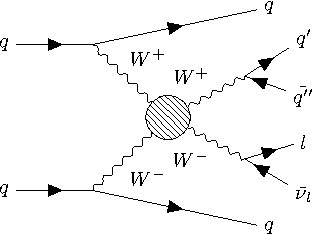
\includegraphics[width=0.33\textwidth]{Images/VBS_Studies/Figure_001-a.pdf}
  \hspace{2cm}
  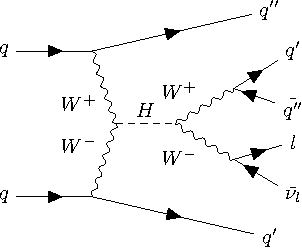
\includegraphics[width=0.33\textwidth]{Images/VBS_Studies/Figure_001-b.pdf}
  \vspace{1cm}
  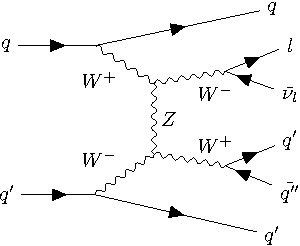
\includegraphics[width=0.33\textwidth]{Images/VBS_Studies/Figure_001-c.pdf}
  \hspace{2cm}
  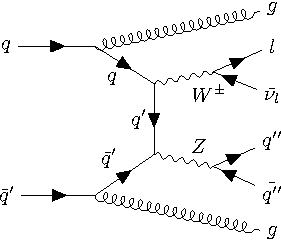
\includegraphics[width=0.33\textwidth]{Images/VBS_Studies/Figure_001-d.pdf}

\caption{Examples of Feynman diagrams contributing to the analyzed final state:
general schema of purely EW VBS signal process contributions (upper
left diagram), the $s$-channel Higgs boson contribution (upper right
diagram), the purely EW nonresonant diboson production (lower left
diagram); and an example of non-EW nonresonant diboson production
(lower right diagram), which is part of the irreducible background. } \label{fig:diagram}
\end{figure*}


Both ATLAS and CMS Collaborations have already studied the VBS $\PW\PV$ process, where {\PV} stands for a {\PW} or {\PZ}
boson, in final states where one boson decays leptonically, and the other boson decays hadronically, with data collected
in 2016, corresponding to only one quarter of the full Run~2 dataset obtained from 2016 to 2018.  The CMS
analysis~\cite{Sirunyan:2019der} was focused on a search for anomalous EW $\PW\PV$ production and put stringent limits
on effective field theory operators, whereas the ATLAS paper~\cite{Aad:2019xxo} reached a SM signal significance of 2.7
standard deviations including the $\ell\ell\PQq\PQq$ and $\nu\nu\PQq\PQq$ decay channels. ATLAS also studied
anomalous couplings in the $\PW\PW/\PW\PZ jj$ channel~\cite{ATLAS:2016nmw} using 8 TeV data from the 2012 dataset.
This paper reports the first evidence for the SM EW $\ell\nu\PQq\PQq$
plus two jets production by analyzing the full LHC
data set collected by CMS between 2016 and 2018, corresponding to an
integrated luminosity of $138\fbinv$.

\section{Signal and background simulation}\label{sec:2}

The signal is characterized by the presence of a single isolated electron or muon, a moderate amount of missing
transverse momentum \ptmiss, and either three or four jets.  One pair of jets is required to have a large invariant mass
and large pseudorapidity ($\eta$) separation, the typical signature of VBS-like events, whereas the remaining jets are
the result of a vector boson decay.  If the boson has a high enough momentum in the laboratory reference frame, its
decay products can be collected in a single jet, whereas at lower momentum the decay is resolved into two separate jets.

The main sources of background contamination originate from the production of a single {\PW} boson accompanied by jets
(called {\PW}+jets in the following), and \ttbar pairs, where one of the {\PW} bosons produced by the top quark decays
hadronically.  Although simulated samples for these backgrounds are available, an approach based on control samples from
data is applied to improve the description of these backgrounds in the signal region.  The {\PW}+jets contribution from
Monte Carlo (MC) is corrected differentially by exploiting the events in a dedicated control region, which is described
in more detail in Section~\ref{sec:5}. The kinematic distributions of the top quark background are taken
from MC, but the normalization is measured from data in the dedicated control region.

The following background processes are modeled using MC event generators: nonresonant QCD-associated diboson production
(QCD-$\PW\PV$);
\ttbar and single top quark production (in $s$, $t$ channel and $\PQt\PW$);
Drell--Yan (DY) lepton pair production; {\PV} boson production in association with a photon (\wg and \zg); single vector
boson EW production in the vector boson fusion channel (VBF-{\PV}); and triboson production ($\PV\PV\PV$).  The QCD
multijet background, which may enter the signal region with nonprompt leptons, is estimated instead in a purely
data-driven method, as described in Sec.~\ref{sec:5}.

Most of the processes are simulated at next-to-leading order (NLO) in the strong coupling $\alpha_{s}$ using
\POWHEG~v2~\cite{Frixione:2002ik,Nason:2004rx,Frixione:2007vw,Alioli:2008gx,Alioli:2010xd}, 
\MGvATNLO v2.4.2 ~\cite{Alwall:2014hca,Alwall:2007fs}, 
or \MCFM~v7.0~\cite{campbell_precision_2019,campbell_multi-threaded_2015,campbell_vector_2011,campbell_update_1999}. 
Only the {\PW}+jets, QCD-$\PV\PV$, VBF-{\PV}, and \wg events are generated with \MGvATNLO v2.4.2 at leading order (LO)
accuracy in perturbative quantum chromodynamics (QCD).  The \ttbar component of the top quark background and the DY
events are also weighted using generator level information to improve the agreement of the simulated transverse momentum
(\pt) distributions of the \ttbar and DY systems~\cite{Czakon:2017wor,CMS:2016oae,CMS:2019raw} to data.

The signal, namely the VBS $\PW(\ell\nu)\PV(\mathrm{jj})$ process (the parentheses give the decay modes), is simulated
with \MGvATNLO v2.6.5 at leading order: the intermediate-state vector boson pair is produced by implementing the narrow
width approximation and then decayed by MadSpin~\cite{Madspin} to partially account for finite-width effects and spin
correlations.  The contribution from the VBS $\PZ(\ell\ell)\PV(\mathrm{jj})$ production, where one of the leptons falls
beyond the acceptance of the analysis, is considered as a background.  The {\PW} decay into \PGt is considered part of
the signal, and {\PW} decays into all leptonic final states are generated. However, the analysis has been performed
only for electron and muon final states.

Apart from VBF-{\PV}, all MC samples for the parton showering, hadronization, and the simulation of the underlying event
are provided by \PYTHIA~8.226 (8.230) \cite{Sjostrand:2014zea,Alioli:2010xd}.  The NNPDF 3.0 NLO \cite{Ball:2014uwa}
(NNPDF 3.1 NNLO \cite{Ball:2017nwa}) parton distribution functions (PDFs) are used for simulating all 2016 (2017 and
2018) samples.  The modeling of the underlying event is generated using the CUETP8M1 \cite{Skands:2014pea,CMS:2015wcf}
(CP5 \cite{CMS:2019csb}) tune for simulated samples corresponding to the 2016 (2017 and 2018) data.

To improve the description of the additional jet emissions by the parton shower simulation in the VBS
topology~\cite{covarelli_vector-boson_2021,ballestrero_precise_2018,Jager:2020hkz}, the dipole recoil scheme is used in
 \PYTHIA for the VBS signal MC sample, and the \HERWIG~7.0~\cite{Bahr:2008pv,Bellm:2015jjp}
program is used for the VBF-{\PV} background.

The interference between the EW and QCD diagrams for the $\PW^{\pm}\PW^{\pm}$, $\PW^{\pm}\PW^{\mp}$, and $\PW\PZ$
 processes, generated with $\MGvATNLO$ including the contributions of order $\alpS\alpha_{\mathrm{EM}}^5$, is less than
 3\% of the signal inclusively in the phase space region of interest of the analysis and is neglected.
 
For all processes, the detector response is simulated using a detailed description of the CMS detector, based on
the \GEANTfour package~\cite{Agostinelli:2002hh}.  Additional interactions in the same or adjacent bunch crossings
(pileup) based on minimum bias events simulated with the \PYTHIA
shower simulation are overlaid onto each event, with the number of
interactions drawn from a distribution that is similar to the one observed in data.  The average number of such
interactions per event is $\approx$23 and $\approx$32 for the 2016 data and 2017-2018 data, respectively.


% \section{The CMS detector}\label{sec:3}

% A detailed description of the CMS detector, together with a definition of the coordinate system used and the relevant
% kinematic variables, can be found in Ref.~\cite{Chatrchyan:2008zzk}.

% The central feature of the CMS apparatus is a superconducting solenoid of 6\unit{m} internal diameter, providing a
% magnetic field of 3.8\unit{T}. Within the solenoid volume are a silicon pixel and strip tracker, a lead tungstate
% crystal electromagnetic calorimeter (ECAL), and a brass and scintillator hadron calorimeter (HCAL), each composed of a
% barrel and two endcap sections. Forward calorimeters extend the pseudorapidity coverage provided by the barrel and
% endcap detectors. Muons are measured in gaseous detectors embedded in the steel flux-return yoke outside the solenoid.
% The particle-flow algorithm~\cite{CMS-PRF-14-001} reconstructs and identifies each individual particle in an event, with
% an optimized combination of information from the various elements of the CMS detector.  The energy of photons is
% obtained from the ECAL measurement.  The energy of electrons is determined from a combination of the electron momentum
% at the primary interaction vertex as measured by the tracker, the energy of the corresponding ECAL cluster, and the
% energy sum of all bremsstrahlung photons spatially compatible with originating from the electron track.  The energy of
% muons is obtained from the curvature of the corresponding track.  The energy of charged hadrons is determined from a
% combination of their momentum measured in the tracker and the matching ECAL and HCAL energy deposits, corrected for the
% response function of the calorimeters to hadronic showers.  Finally, the energy of neutral hadrons is obtained from the
% corresponding corrected ECAL and HCAL energies.

% Events of interest are selected using a two-tiered trigger system.  The first level, composed of custom hardware
% processors, uses information from the calorimeters and muon detectors to select events at a rate of up to 100\unit{kHz}
% within a fixed latency of about 4\mus~\cite{Sirunyan:2020zal}.  The second level, known as the high-level trigger,
% consists of a farm of processors running a version of the full event reconstruction software optimized for fast
% processing, and reduces the event rate to around 1\unit{kHz} before data storage~\cite{Khachatryan:2016bia}.

\section{Event reconstruction, selection and categorization}\label{sec:4}

Events are selected for further analysis by triggers for isolated single leptons with \pt thresholds of 27, 32, 35\GeV
for electrons and of 24, 24, 27\GeV for muons, respectively for the 2016, 2017, 2018 data-taking periods.  The final
leptons are required to have an offline reconstructed \pt of at least $35\GeV$ ($30\GeV$) for electron (muon)
candidates, and a pseudorapidity of $\abs{\eta}<2.5$ (2.4) for electrons (muons).

For each event, hadronic jets are clustered from reconstructed particles using the infrared- and collinear-safe anti-\kt
algorithm~\cite{Cacciari:2008gp, Cacciari:2011ma} with a distance parameter of 0.4 (0.8), labeled in the following as
AK4 (AK8) jets.  Additional proton-proton interactions within the same or nearby bunch crossings (pileup) can contribute
additional tracks and calorimetric energy depositions to the jet momentum.  To mitigate this effect, charged particles
identified as originating from pileup vertexes are discarded and an offset correction is applied to correct for
remaining contributions. Reconstructed jets cannot overlap with isolated leptons:
$\Delta R(j, \ell)= \sqrt{\smash[b]{(\Delta\eta)^2 + (\Delta\phi)^2}} >$ 0.4 (0.8) for AK4 (AK8) jets. 

In an event, AK4 and AK8 jets are considered in the analysis if they have a $\pt>30\GeV$ and $\abs{\eta}<4.7$ or
$\pt>200\GeV$ and $\abs{\eta}<2.4$, respectively.  The pileup-per-particle identification algorithm
(PUPPI)~\cite{Sirunyan:2020foa,Bertolini:2014bba} is applied to AK8 jet constituents to remove pileup tracks at the
reconstructed particle level.  Moreover, a grooming algorithm, known as ``soft drop''
(SD)\cite{Dasgupta:2013ihk,Butterworth:2008iy,Larkoski:2014wba}, is applied to the constituents of AK8 jets reclustered
using the Cambridge--Aachen algorithm~\cite{Dokshitzer:1997in,Wobisch:1998wt}.  The SD algorithm, which has as an
angular exponent $\beta = 0$, soft cutoff threshold $z_{\text{cut}} < 0.1$, and characteristic radius $R_{0} =
0.8$~\cite{Larkoski:2014wba}, removes soft, wide-angle radiation from the large radius jet, improving the modeling of
the jet mass observable.  The parameters of the SD algorithm are calibrated in a top quark-antiquark sample enriched in
hadronically decaying $\PW$ bosons~\cite{Khachatryan:2014vla}.  The AK8 jets are identified as hadronic decays of
Lorentz-boosted $\PW/\PZ$ bosons using the ratio between 2- and 1-subjettiness~\cite{Thaler:2010tr} variables denoted as
$\tau_{21}=\tau_{2}/\tau_{1} < 0.45$ and a groomed AK8 jet mass between 40 and 250\GeV. AK4 jets overlapping
with AK8 jets that pass the preselection with $\Delta R(j_{\text{AK4}}, j_{\text{AK8}}) < 0.8$ are removed from the event.  

The analysis targets the VBS production of pairs of vector bosons, $\PW\PV$, in association with two jets originating
from the scattered incoming partons, called tag jets.  In the chosen signal process, the {\PW} boson decays leptonically
and the second boson decays hadronically.  Candidate events are required to contain exactly one tightly identified and
isolated lepton \cite{Khachatryan:2015hwa,Chatrchyan:2012xi} associated with the {\PW} boson leptonic decay. Events
containing a second loosely identified lepton with $\pt > 10\GeV$ are vetoed.  Finally, we require a missing transverse
momentum $\ptmiss > 30\GeV$ in the event.  The missing transverse momentum vector \ptvecmiss is computed as the negative
vector sum of the transverse momenta of all the particle candidates in an event~\cite{Sirunyan:2019kia}.  The PUPPI
algorithm is also applied to reduce the pileup dependence of the \ptmiss observable. The \ptmiss vector is computed from
the particle-flow candidates weighted by their probability to originate from the primary interaction
vertex~\cite{Sirunyan:2019kia}.

Two main categories are defined depending on the reconstruction regime of the hadronically decaying vector boson.  An
event is assigned to a boosted category if it contains only one AK8 jet, with $\pt > 200\GeV$ and $|\eta|<2.4$, that
passes the selection criteria as a hadronically decaying vector boson \vhad, together with at least two AK4
jets. Otherwise, if no AK8 jet V boson candidate is found and instead at least four AK4 jets are reconstructed with $\pt
> 30\GeV$, the event is assigned to a resolved category.  In both resolved and boosted categories, the two AK4 jets with
the largest invariant mass are identified as the VBS tag jets.  In the resolved category, out of the remaining jets
after the VBS tag jet selection, the two jets with invariant mass closest to $85\GeV$ (the average between the {\PW} and
{\PZ} boson masses) are chosen as the decay product of \vhad.

The fraction of VBS events in the sample is enhanced requiring a large invariant mass $\mjjvbs > 500\GeV$ and large
pseudorapidity interval $\detavbs= | \eta_{j1}^{\text{VBS}} - \eta_{j2}^{\text{VBS}}| > 2.5$ for the tag jets.  The
leading VBS tag jet is required to have $\pt > 50\GeV$ and the transverse mass of the leptonically decaying {\PW} is
required to be $\mtw < 185\GeV$, defined as
\begin{linenomath}
\begin{equation}
\mtw = \sqrt{2\,\pt(\ell) \ptmiss [ 1 - \cos (\Delta\varphi (\pt(\vec{\ell}), \ptvecmiss))]}~,
\end{equation}
\end{linenomath}
where $\pt(\ell)$ is the \pt of the lepton and $\Delta\varphi (\pt(\vec{\ell}), \ptvecmiss)$ is the azimuthal distance
between the lepton and the \ptvecmiss.

After these selections, the signal and control regions for the main backgrounds, the top quark and {\PW}+jets ones, are
defined in both the resolved and boosted regions in a similar manner.

The signal region consists of events where:
(i) no {\PQb} jet candidates are found according to the loose working point
of the \textsc{DeepCSV} tagger~\cite{Sirunyan:2017ezt},
(ii) a machine-learning {\PQb}-tagging algorithm with a
{\PQb}-tagging efficiency $\ge85\%$ and a mistag probability $\le20\%$ reduces the contamination
from \ttbar events,
and (iii) the hadronically decaying vector boson
invariant mass $\mvhad$ is between $65-105$ ($70-115$)\GeV for the resolved (boosted) category, which is consistent with
an on-shell {\PW} or {\PZ} decaying hadronically.  Events falling in the same $\mvhad$ interval as the signal but
containing at least one {\PQb} jet are classified in the top quark control region.  Finally, if no {\PQb} jets exist and
$\mvhad$ is not within the $\PW$ or $\PZ$ resonance range, $\mvhad\notin(65 , 105)\GeV$ or $\mvhad\notin(70 , 115)\GeV$
for the resolved and boosted cases, events are classified as part of the {\PW}+jets control region.  All of the signal
and control regions are split according to the flavor of the selected lepton (electron or muon).


\section{Background estimation}\label{sec:5}

The largest background contribution is the {\PW}+jets process, followed by the top quark and the QCD multijet
backgrounds. The contamination from the single vector boson EW production in the VBF channel (VBF-{\PV}) is negligible
in the resolved category (2\% inclusively), but more important in the boosted one (4\% inclusively).

The {\PW}+jets contribution is corrected using control samples in data.  It is experimentally observed that the
transverse momentum of the leptonically decaying {\PW} boson (\wlpt), measured using the lepton momentum and
the \ptmiss, and the VBS tag jets \pt are poorly described by simulation in the multijet phase space region used in this
analysis.  To correct this important background in a differential way, the {\PW}+jets MC sample is split into several
subsamples according to \wlpt (both categories) and \pt of the subleading VBS tag jet (only in the resolved category),
and their normalizations are left floating and uncorrelated in the final fit. The data in the {\PW}+jets control region is used
to constrain the normalization of the {\PW}+jets subcomponents by including in the fit the same variables
with the same binning used to defined the MC sample splitting.
As a result of this procedure, the normalization corrections to the W+jets MC
sample are propagated in the fit and also to the signal region including the full covariance matrix.

The closure test for this correction is performed by dividing the {\PW}+jets control region into two subregions, defined
by two intervals of \mvhad closer to (\ie, $[50,65] \cup [105,150] \GeV$ in the resolved category or $[50,70] \cup
[115,150] \GeV$ in the boosted one) or farther (\ie, $[40, 50] \cup [150,+\infty] \GeV$) from the {\PV} resonance where
the signal region is located.  Correction factors are derived for each {\PW}+jets component in the two subregions and
are in agreement with each other. Therefore, including the {\PW}+jets control region in the final fit to extract the
{\PW}+jets correction factors provides a meaningful description for the {\PW}+jets MC also in the signal region.

The top quark background contribution is determined from MC simulation except for its normalization, which is measured
in the top quark enriched control region in the final fit to the data.

The QCD multijet background, also called nonprompt, is estimated from data by measuring the probability for a loosely
defined reconstructed lepton originating from a jet to be misidentified as a tightly reconstructed lepton in a phase
space region outside the analysis region. The QCD-enriched region is defined by the presence of at least one lepton with
the same \pt requirement as for the rest of the analysis, $\ptmiss < 20\GeV$, $\mtw < 20\GeV$, at least one AK4 jet in
the event with $\Delta R>1$ from the lepton.  The contribution
from EW processes with a real lepton is subtracted from this QCD enriched phase space region by means of {\PW}+jets and
DY MC events.
 
The contributions from the other backgrounds, \eg, QCD-$\PV\PV$, DY, VBF-{\PV}, $\PV\PV\PV$, $\PV\gamma$,
VBS-$\PZ(\ell\ell)\PV(\mathrm{jj})$ processes, are estimated from MC simulation.


\section{Signal extraction}\label{sec:6}

Because of the large background and complex signal topology, the most significant features to separate signal and
backgrounds are condensed in a single discriminator built with a deep neural network (DNN).  This approach increases the
sensitivity of the analysis by a factor of three over a fit to the shape of the most sensitive variable \mjjvbs.
Two different discriminators are optimized for the resolved and boosted categories since the event topology and the
kinematics change significantly between the two.  The DNN implementation consists of a fully connected neural network
with four layers with 64 (32) nodes for the resolved (boosted) topology, trained with stochastic gradient descent
implemented via the ``Adam'' optimizer \cite{kingma_adam:_2017}.  The models are trained minimizing the binary
cross-entropy~\cite{binary_crossentropy,Goodfellow-et-al-2016} loss until full convergence.  All the backgrounds are
included as a single class in the optimization, weighted by their relative importance.  Overfitting is carefully avoided
by the use of regularization techniques, such as Dropout and L2 weights decay \cite{Goodfellow-et-al-2016}.  A technique
called SHAP (SHapley Additive exPlanations) \cite{Lundberg2017,shapley_values}, developed in the field of explainable machine
learning, is applied to cross-check the dependence of the DNN model on the input variables and to rank their importance.
Among the most important ones, as identified by SHAP and matching the physics expectation, are the
\mjjvbs variable, the Zeppenfeld variable \cite{Rainwater:1996ud} of the lepton, and the quark/gluon discriminator 
variable of the leading \vhad jet, which is based on a likelihood discriminant constructed with three variables for
each jet: the jet energy, the multiplicity of the jet constituents, 
and the minor axis width of the ellipse in the $\eta-\phi$ plane containing the jet constituents~\cite{CMS:2013kfa,CMS-DP-2016-070}.

The postfit distribution of the \mjjvbs variable is shown in Fig.~\ref{fig:mjjvbs}.
Table~\ref{tab:variablesDefinition} shows the complete list of input variables used for the resolved and boosted
topologies, along with their ranking from the SHAP algorithm.  The Zeppenfeld variable of a particle X is defined as:
\begin{linenomath}
\begin{equation}
  \mathrm{Z}_{\mathrm{X}} = \frac{\eta^{\mathrm{X}} - \bar{\eta}^{\mathrm{VBS}}}{\detavbs},
\end{equation}
\end{linenomath}
where $\bar{\eta}^{\mathrm{VBS}}$ is the mean pseudorapidity of the VBS tag jets.

The centrality~\cite{atlas_collaboration_measurement_2017,Aaboud:2018ddq} variable is defined as $C_{\PV\PW}
= \min(\Delta\eta_- , \Delta\eta_+)$, with $\Delta\eta_{+} = \max(\eta^{\mathrm{VBS}}) - \max(\eta^{\vhad}, \eta^{\PW})$
and $\Delta\eta_{-} = \min(\eta^{\mathrm{VBS}}) - \min(\eta^{\vhad}, \eta^{\PW})$.  The $\eta^{\PW}$ value is determined
assuming the {\PW} boson mass from the lepton and \ptmiss kinematics.

\begin{table*}[!htb]
\centering
  \topcaption{ Variables used as input to the DNN for the resolved and boosted models.  They are ranked by their
    contributions to the signal discrimination power of the DNN model using the SHAP \cite{Lundberg2017,shapley_values}
    technique and their rank is shown in the table for the resolved and boosted categories
    models.  \label{tab:variablesDefinition} }
\begin{tabular}{l  c c  c c }
\multirow{2}{*}{Variable}        & \multirow{2}{*}{Resolved}   & \multirow{2}{*}{Boosted}  & \multicolumn{2}{c}{SHAP ranking}  \\
 & & & Resolved & Boosted \\
\hline
Lepton pseudorapidity & \checkmark & \checkmark & 13 & 12 \\ Lepton transverse momentum & \checkmark & \checkmark & 16 &
10 \\ Zeppenfeld variable for the lepton & \checkmark & \checkmark & 2 & 2 \\ Number of jets with $\pt > 30\GeV$
& \checkmark & \checkmark & 7 & 3 \\ Leading VBS tag jet \pt & - & \checkmark & - & 11 \\ Trailing VBS tag jet \pt
& \checkmark & \checkmark & 7 & 6 \\ Pseudorapidity interval \detavbs between tag jets & \checkmark & \checkmark & 4 &
4 \\ Quark/gluon discriminator of leading VBS tag jet& \checkmark & \checkmark & 9 & 7 \\ Azimuthal angle distance
between VBS tag jets & \checkmark & - & 10 & - \\ Invariant mass of the VBS tag jets pair & \checkmark & \checkmark & 1
& 1 \\
\pt of the leading \vhad jet  & \checkmark & - & 14 & - \\
\pt of the trailing \vhad jet  & \checkmark & - & 12 & - \\
Pseudorapidity difference between \vhad jets & \checkmark & - & 8 & - \\ Quark/gluon discriminator of the leading \vhad
jet & \checkmark & - & 3 & - \\ Quark/gluon discriminator of the trailing \vhad jet & \checkmark & - & 5 & - \\
\pt of the AK8 \vhad jet candidate   &   -  &  \checkmark   &  - & 8  \\
Invariant mass of \vhad & \checkmark & \checkmark & 11 & 5 \\ Zeppenfeld variable for \vhad & - & \checkmark & - & 9 \\
Centrality & - & \checkmark & 15 & 13 \\
\hline
\end{tabular}
\end{table*}


\begin{figure}[!htpb]
  \centering
  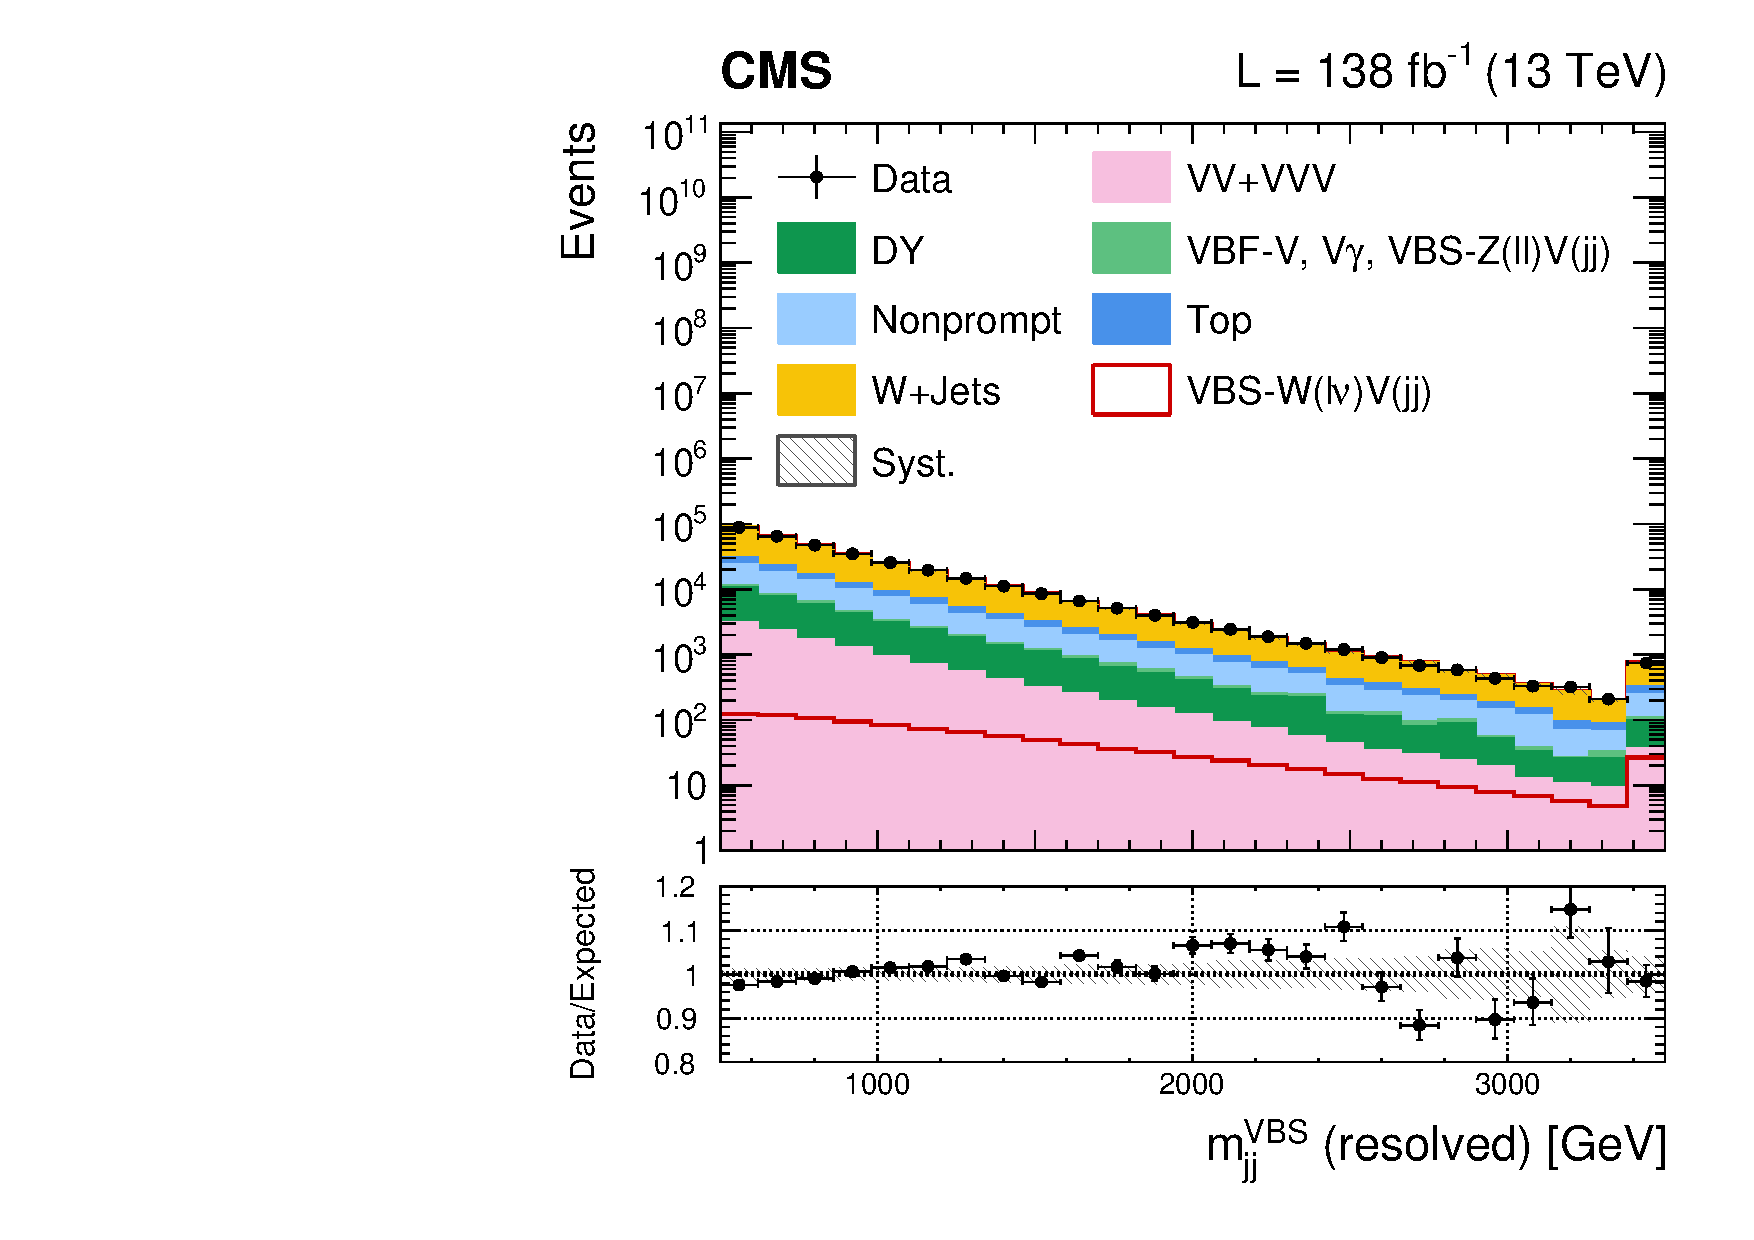
\includegraphics[width=0.49\textwidth]{Images/VBS_Studies/Figure_002-a.pdf}
  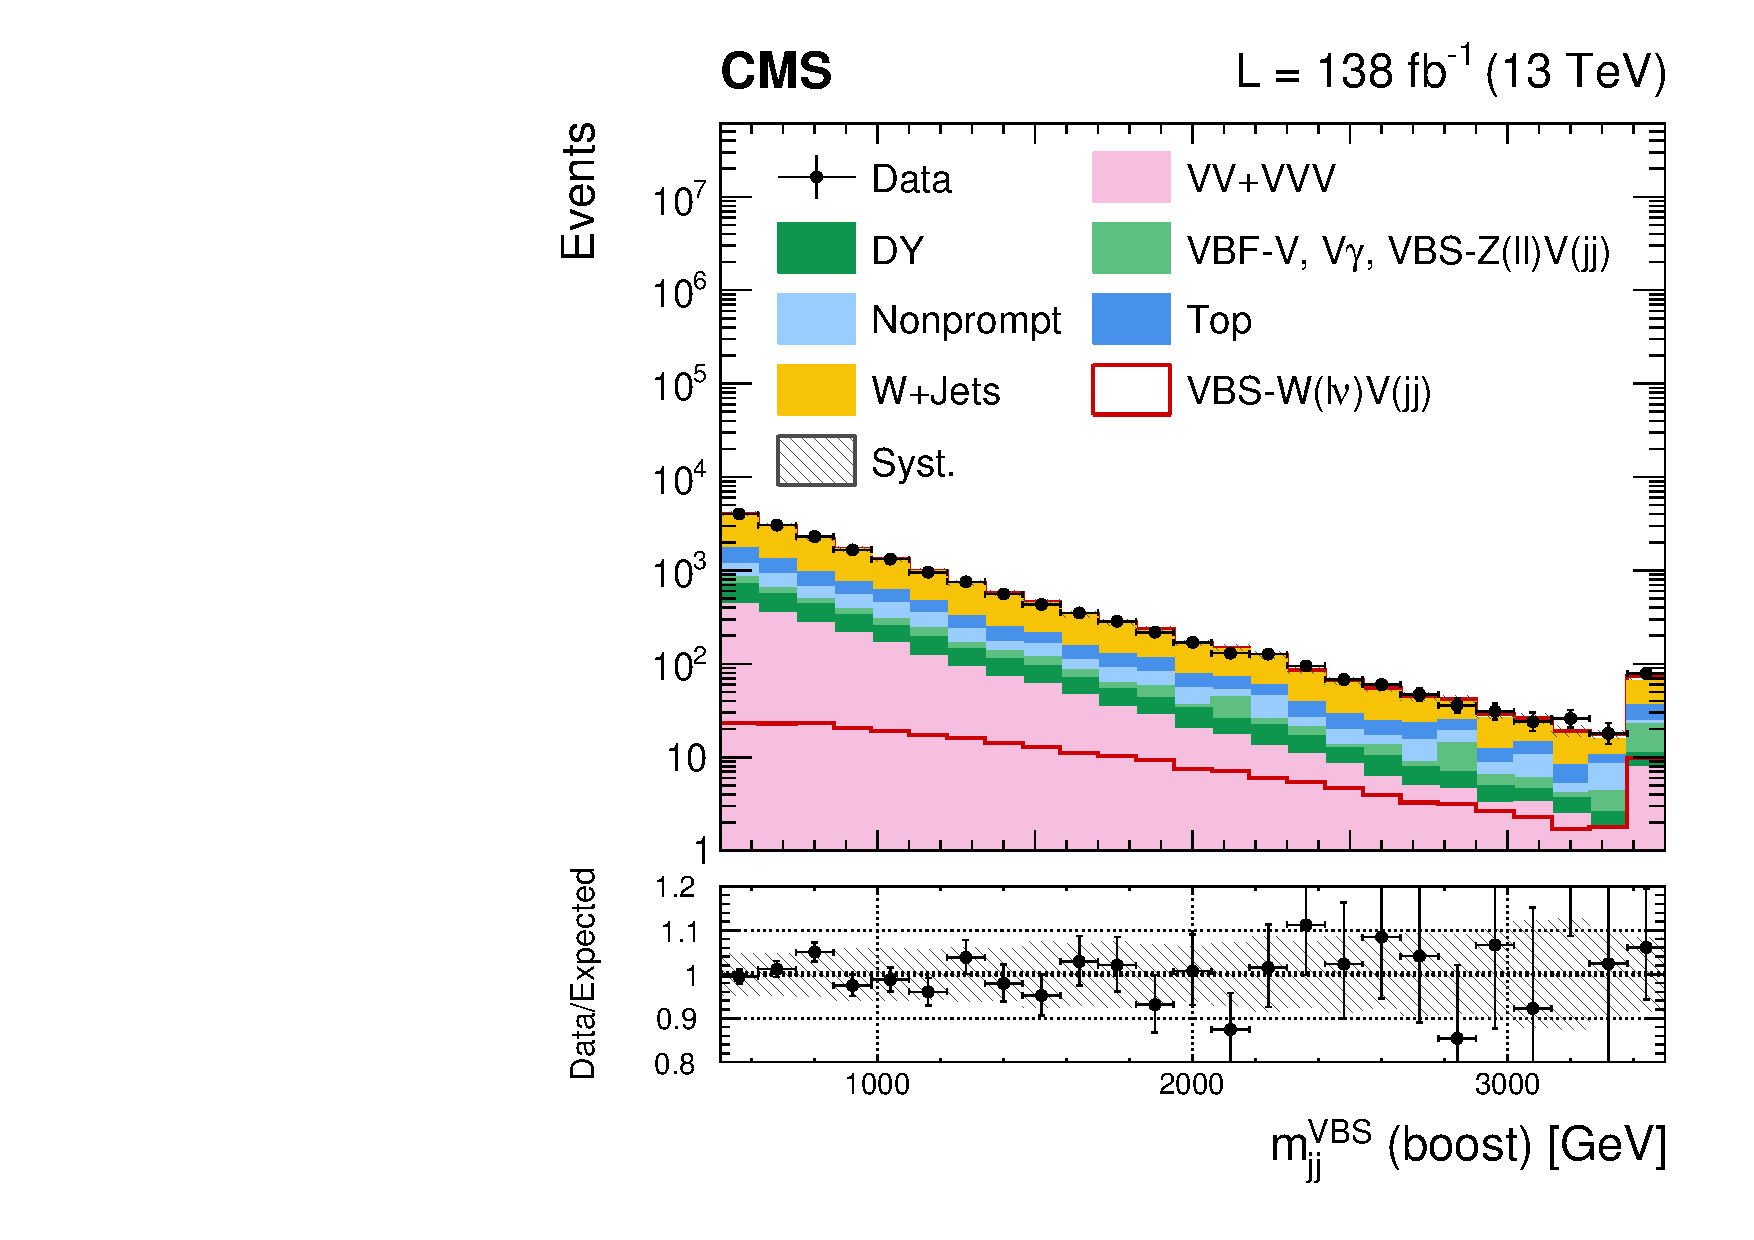
\includegraphics[width=0.49\textwidth]{Images/VBS_Studies/Figure_002-b.pdf}
  \caption{
    Postfit distributions of the \mjjvbs observable in the resolved (\cmsLeft) and boosted (\cmsRight) signal regions.
    Vertical bars on data points show the statistical error, whereas the gray band is the post-fit uncertainty on MC
    with all systematic uncertainties included.  } \label{fig:mjjvbs}
\end{figure}


Fig.~\ref{fig:norm:dnnbin} shows the normalized distributions of the DNN discriminator for signal and backgrounds in the
resolved and boosted signal regions.  Fig.~\ref{fig:CR:dnn} shows control plots for the DNN in the top quark and W+jets
control regions both for the resolved and boosted categories.  The predictions and the data agree within the
uncertainties in both cases, after the background estimation based on control samples in data, as described in the
previous section, is applied.

\begin{figure}[!htb]
  \centering
  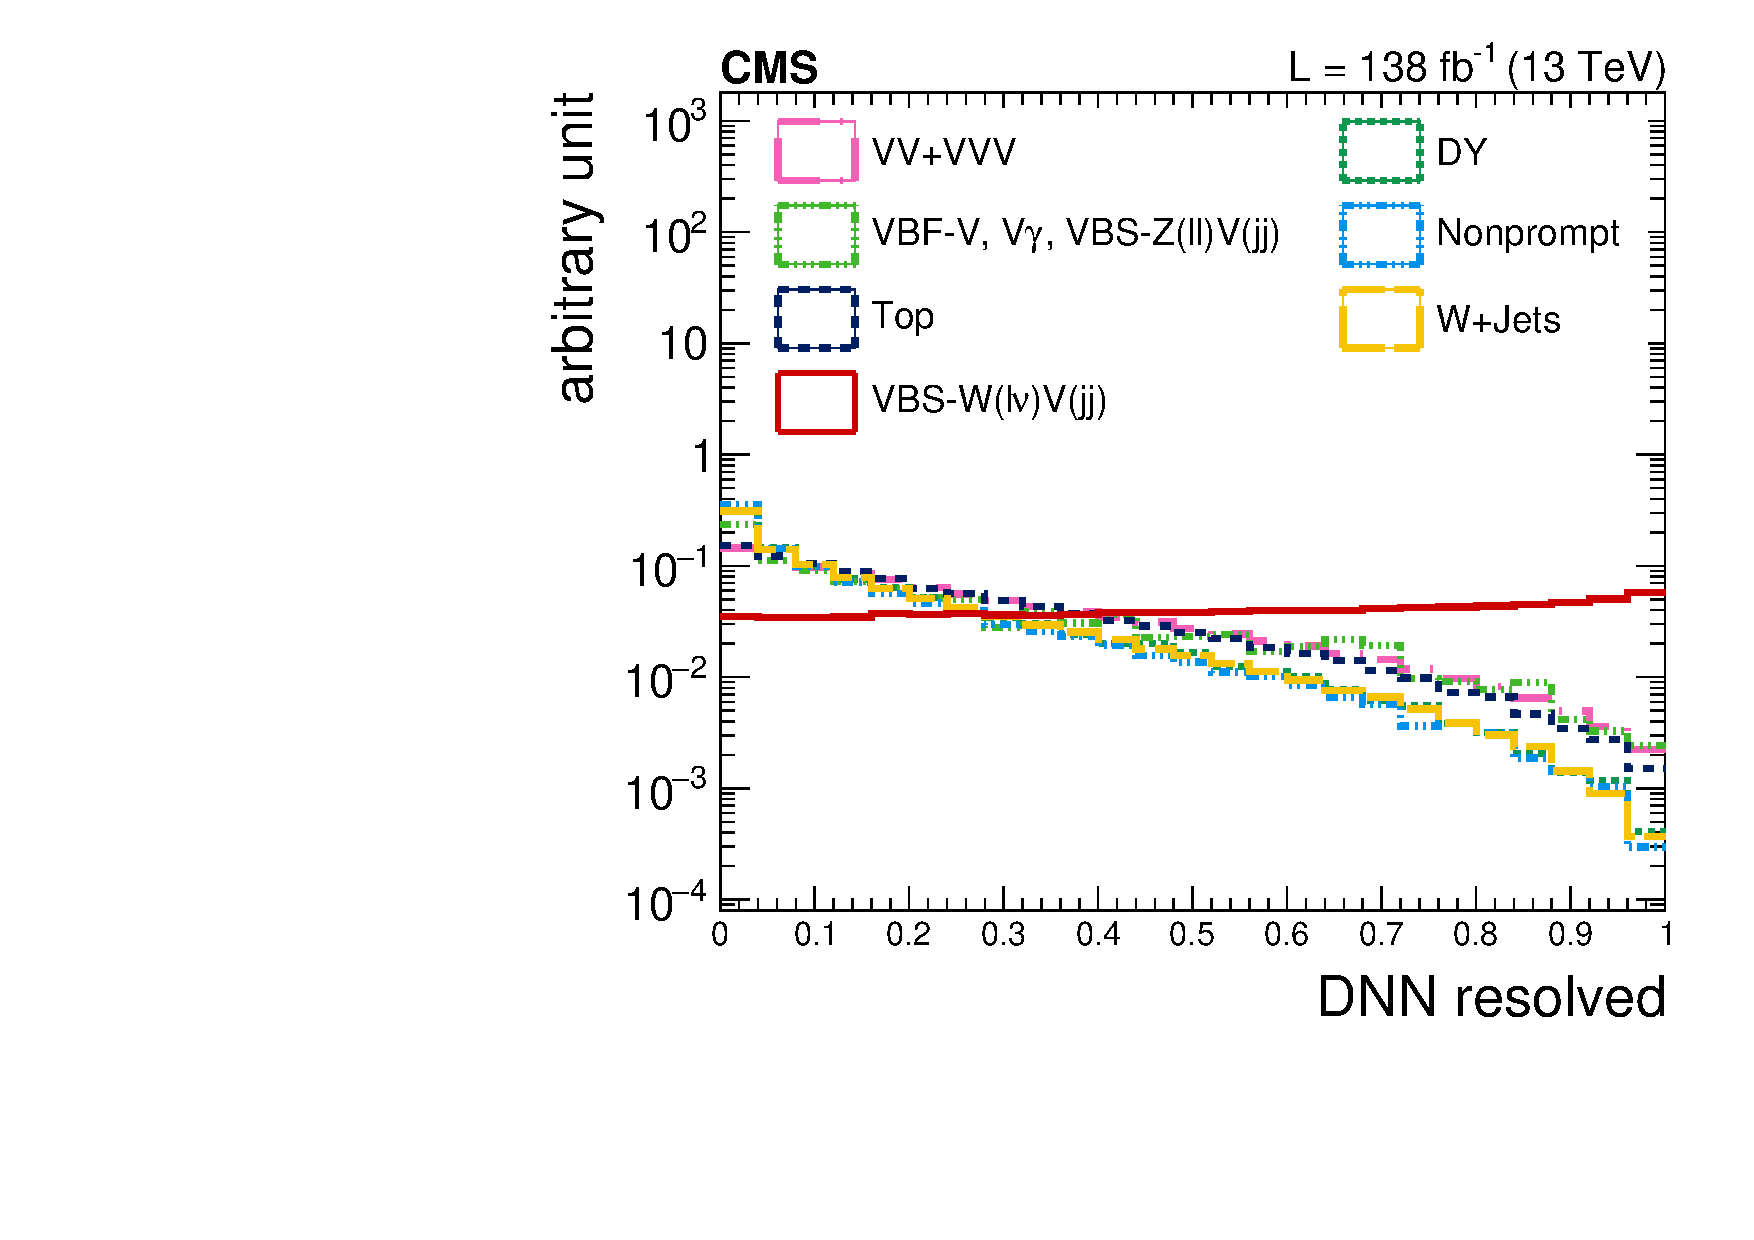
\includegraphics[width=0.49\textwidth]{Images/VBS_Studies/Figure_003-a.pdf}
  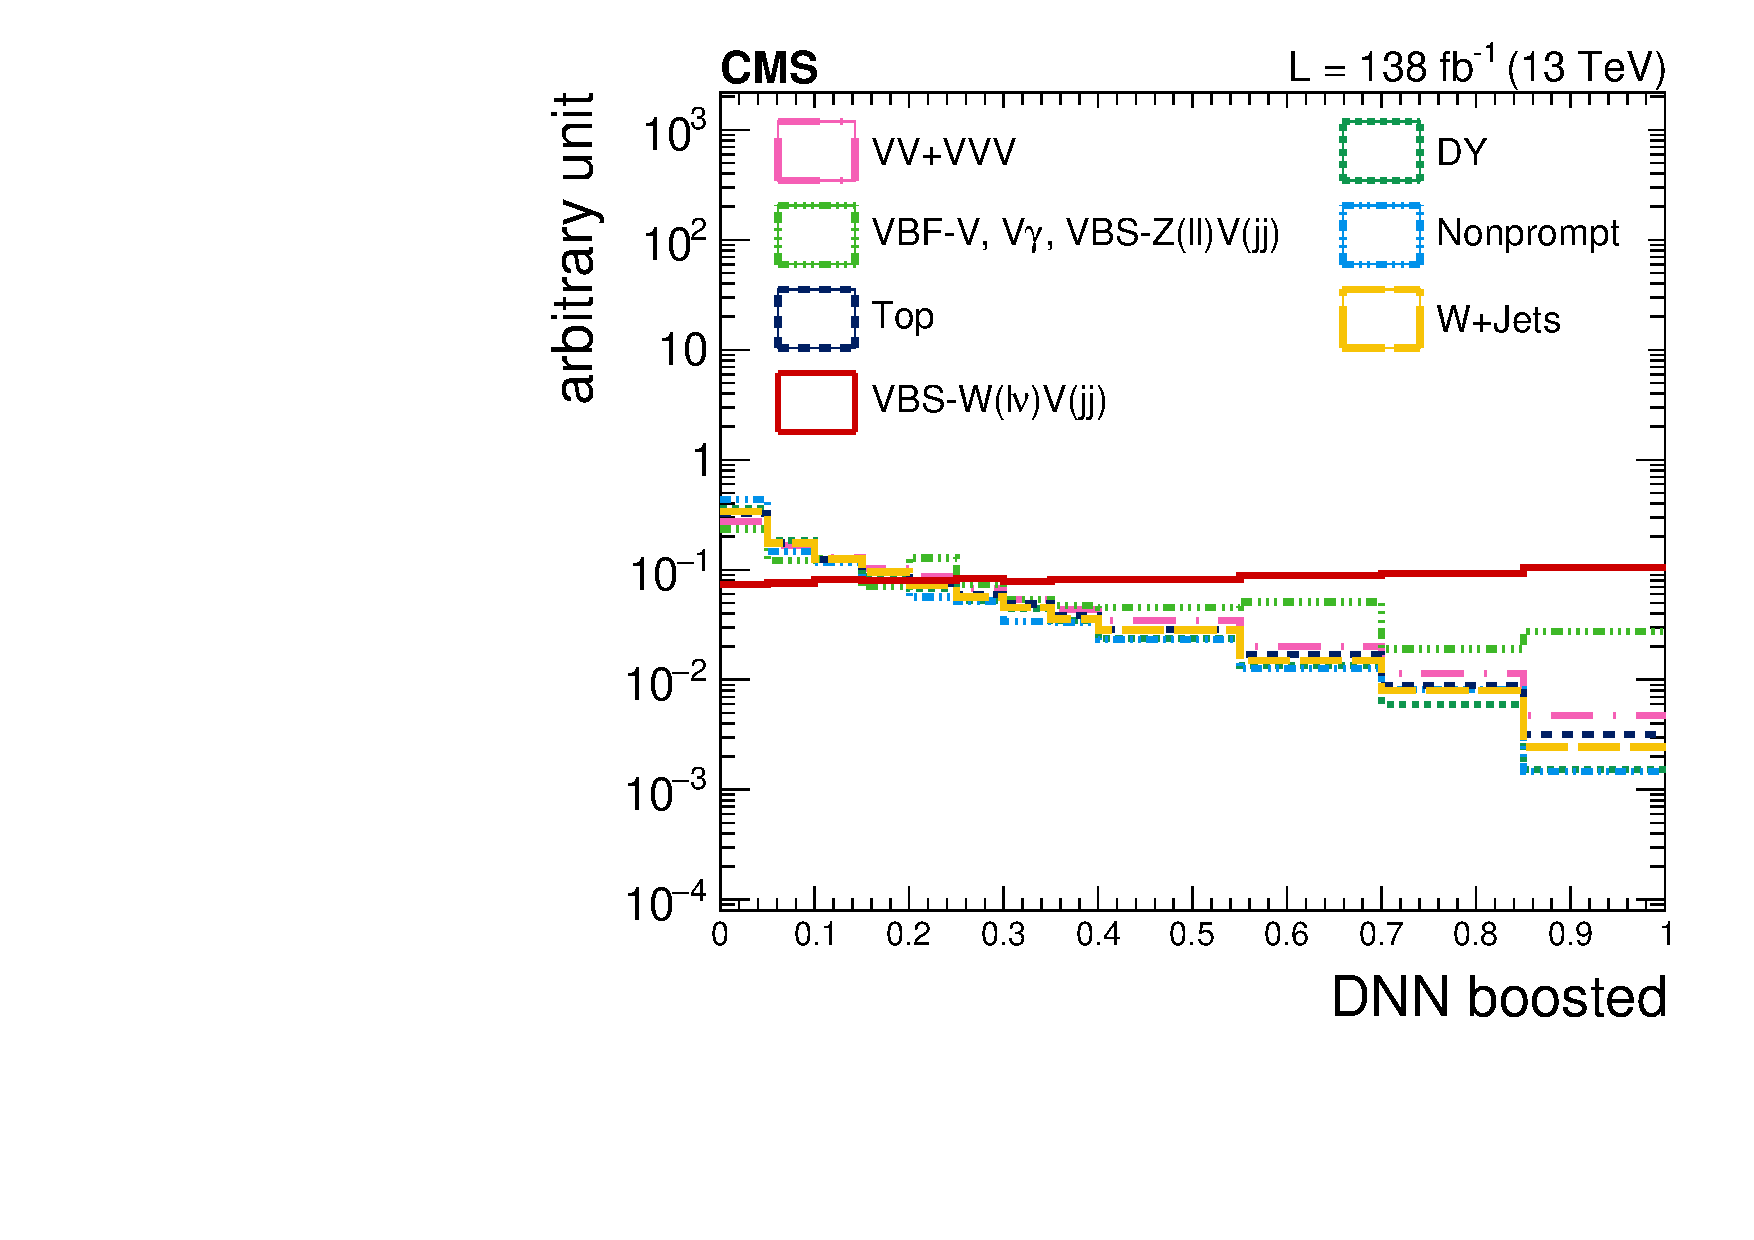
\includegraphics[width=0.49\textwidth]{Images/VBS_Studies/Figure_003-b.pdf}
  \caption{
    The DNN discriminator distribution, taken from simulation, for VBS signal and backgrounds in the resolved (\cmsLeft)
    and boosted (\cmsRight) signal regions normalized to unity.  } \label{fig:norm:dnnbin}
\end{figure}


\begin{figure*}[!htb]
  \centering
  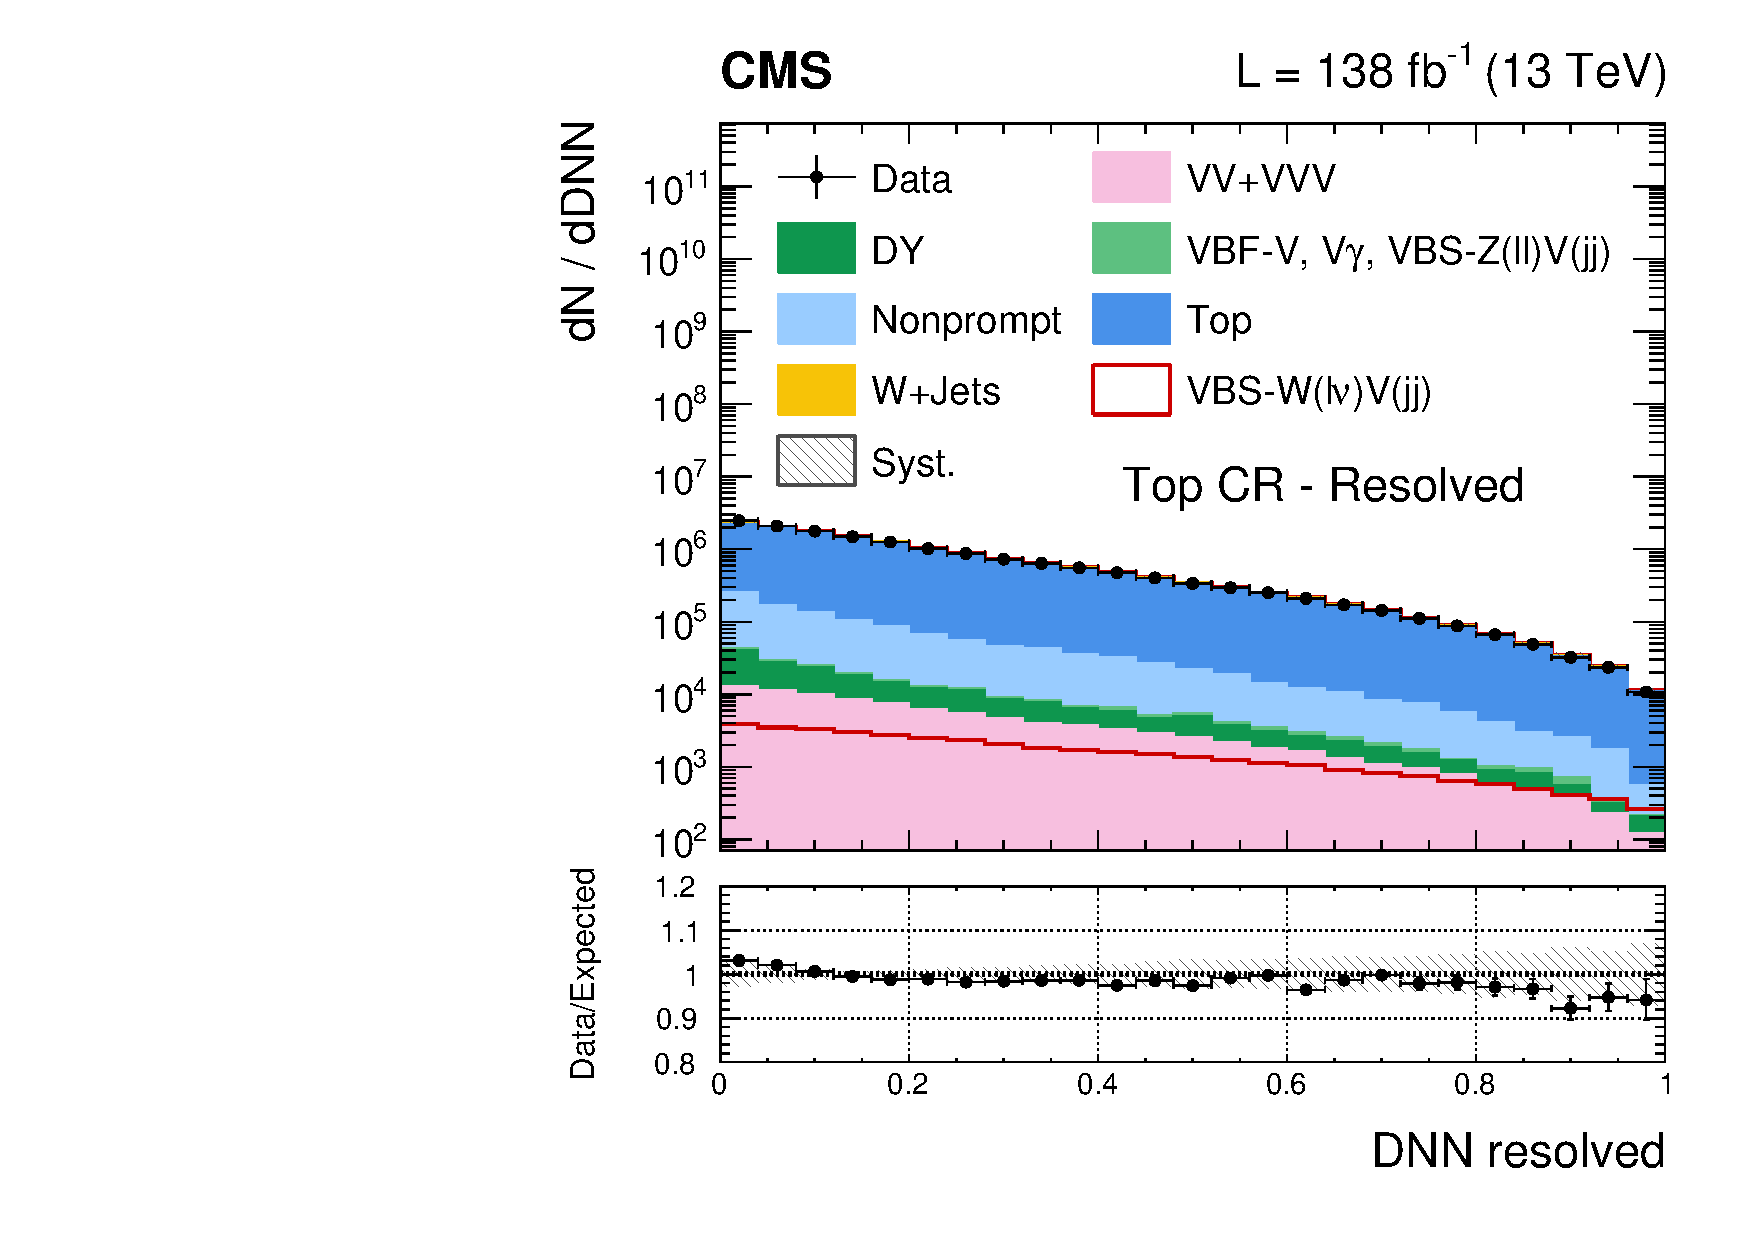
\includegraphics[width=0.49\textwidth]{Images/VBS_Studies/Figure_004-a.pdf}
  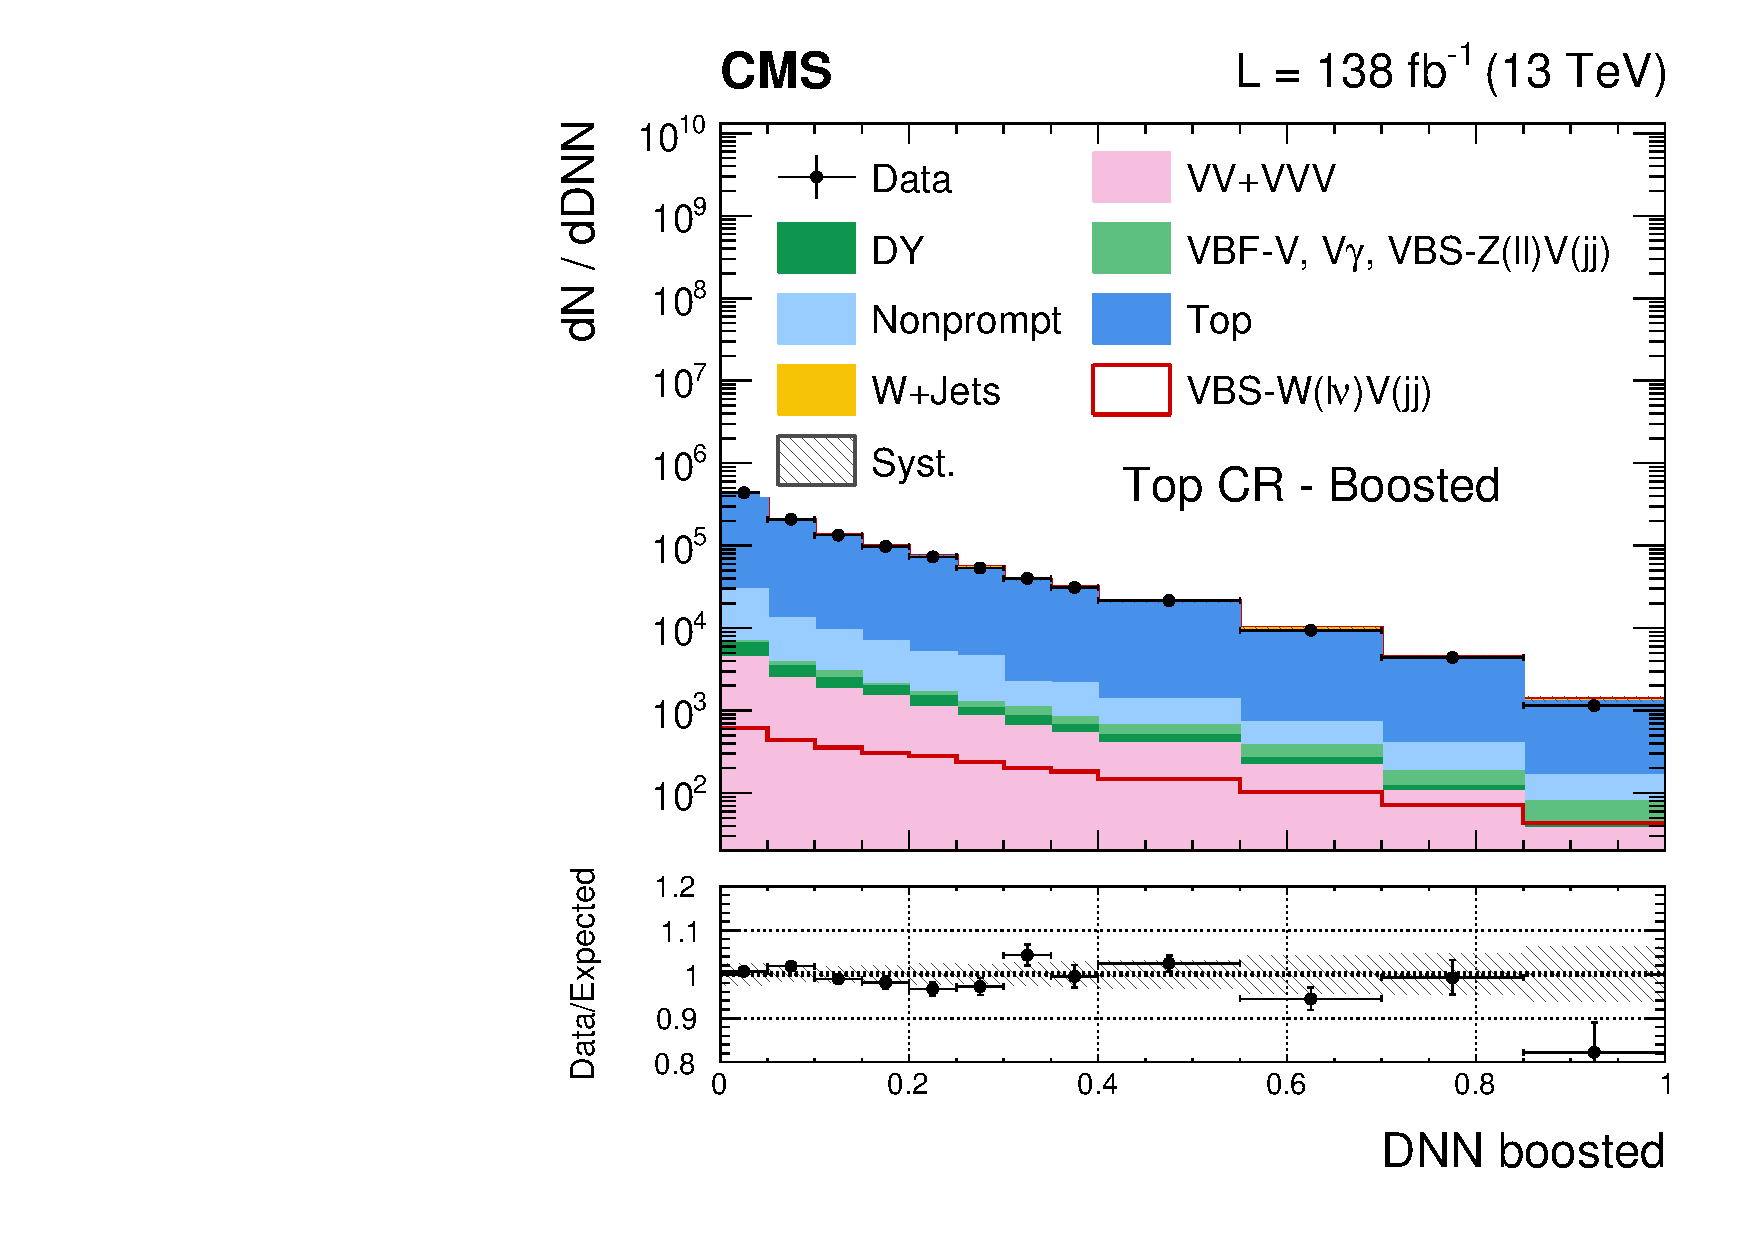
\includegraphics[width=0.49\textwidth]{Images/VBS_Studies/Figure_004-b.pdf}
  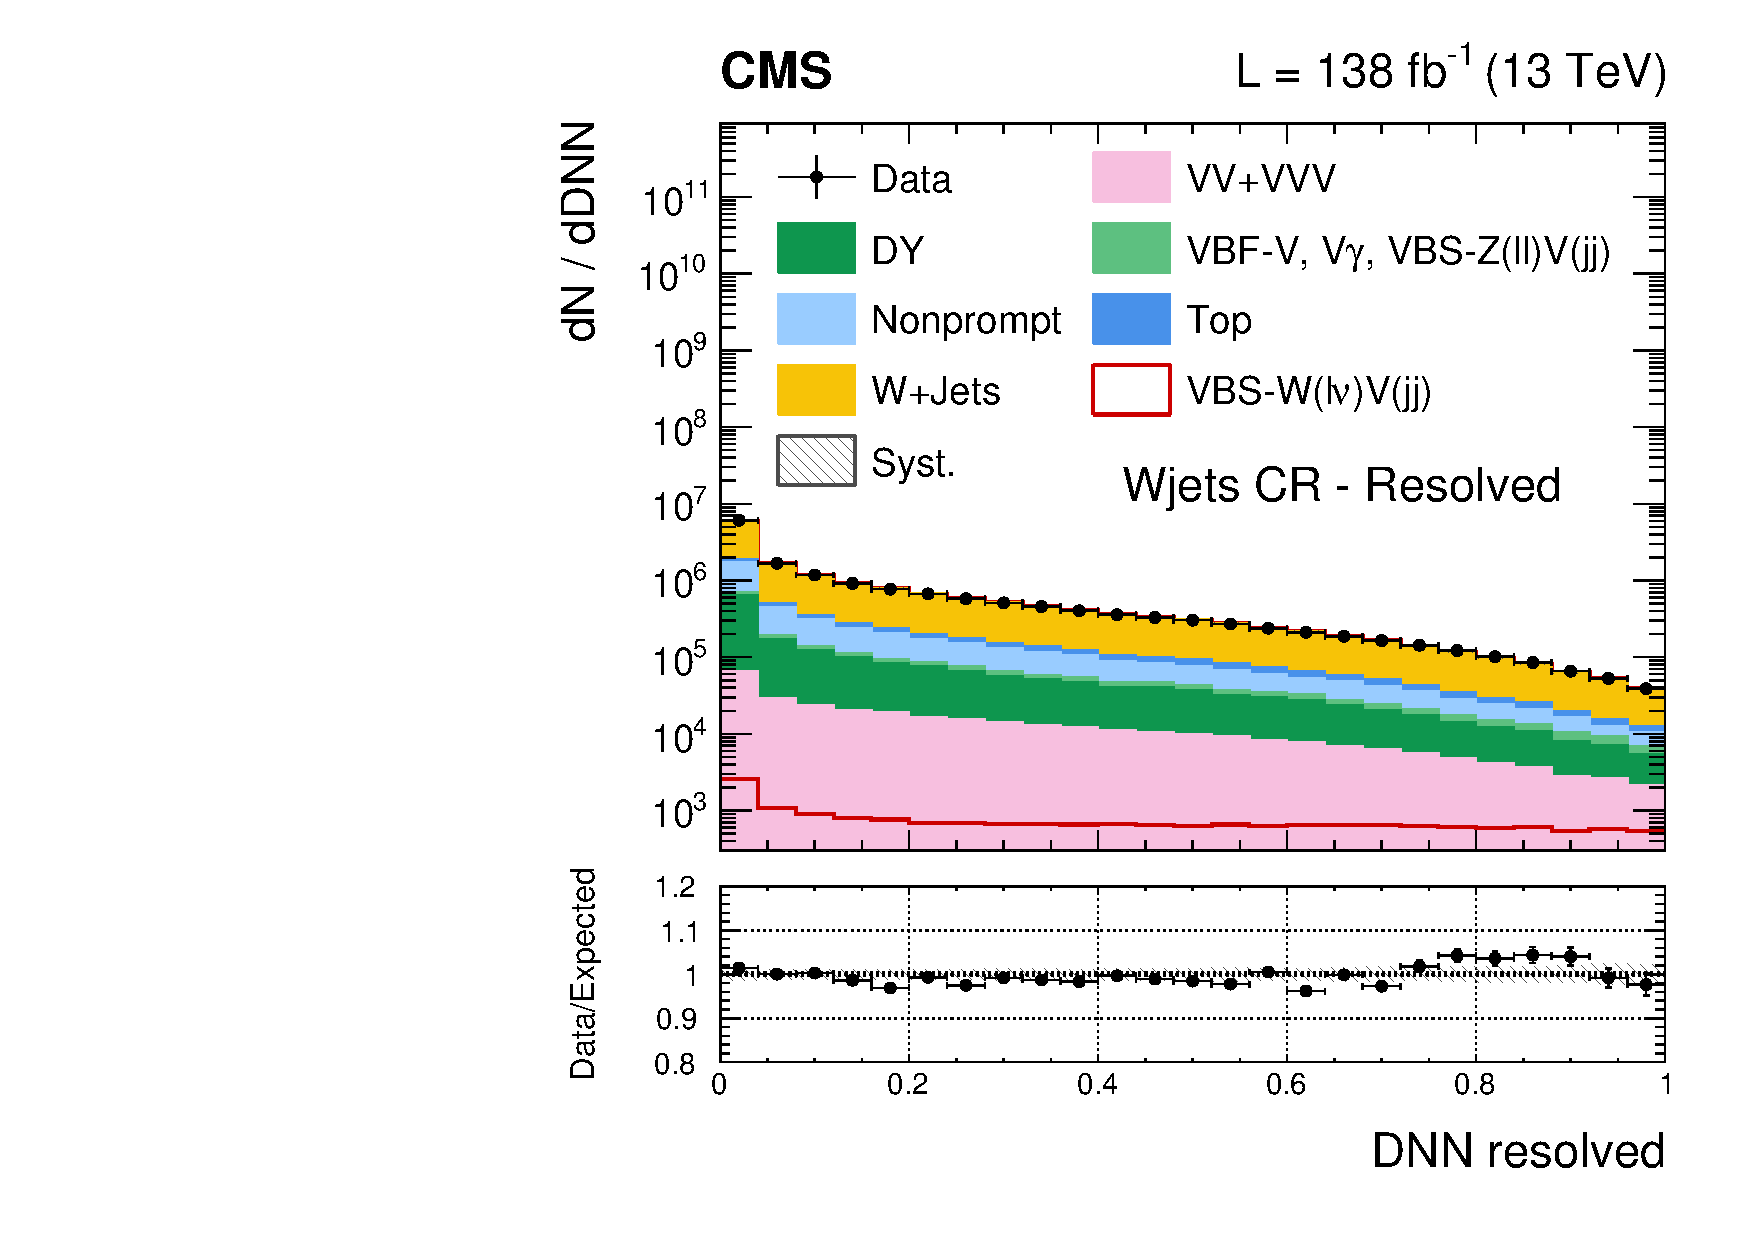
\includegraphics[width=0.49\textwidth]{Images/VBS_Studies/Figure_004-c.pdf}
  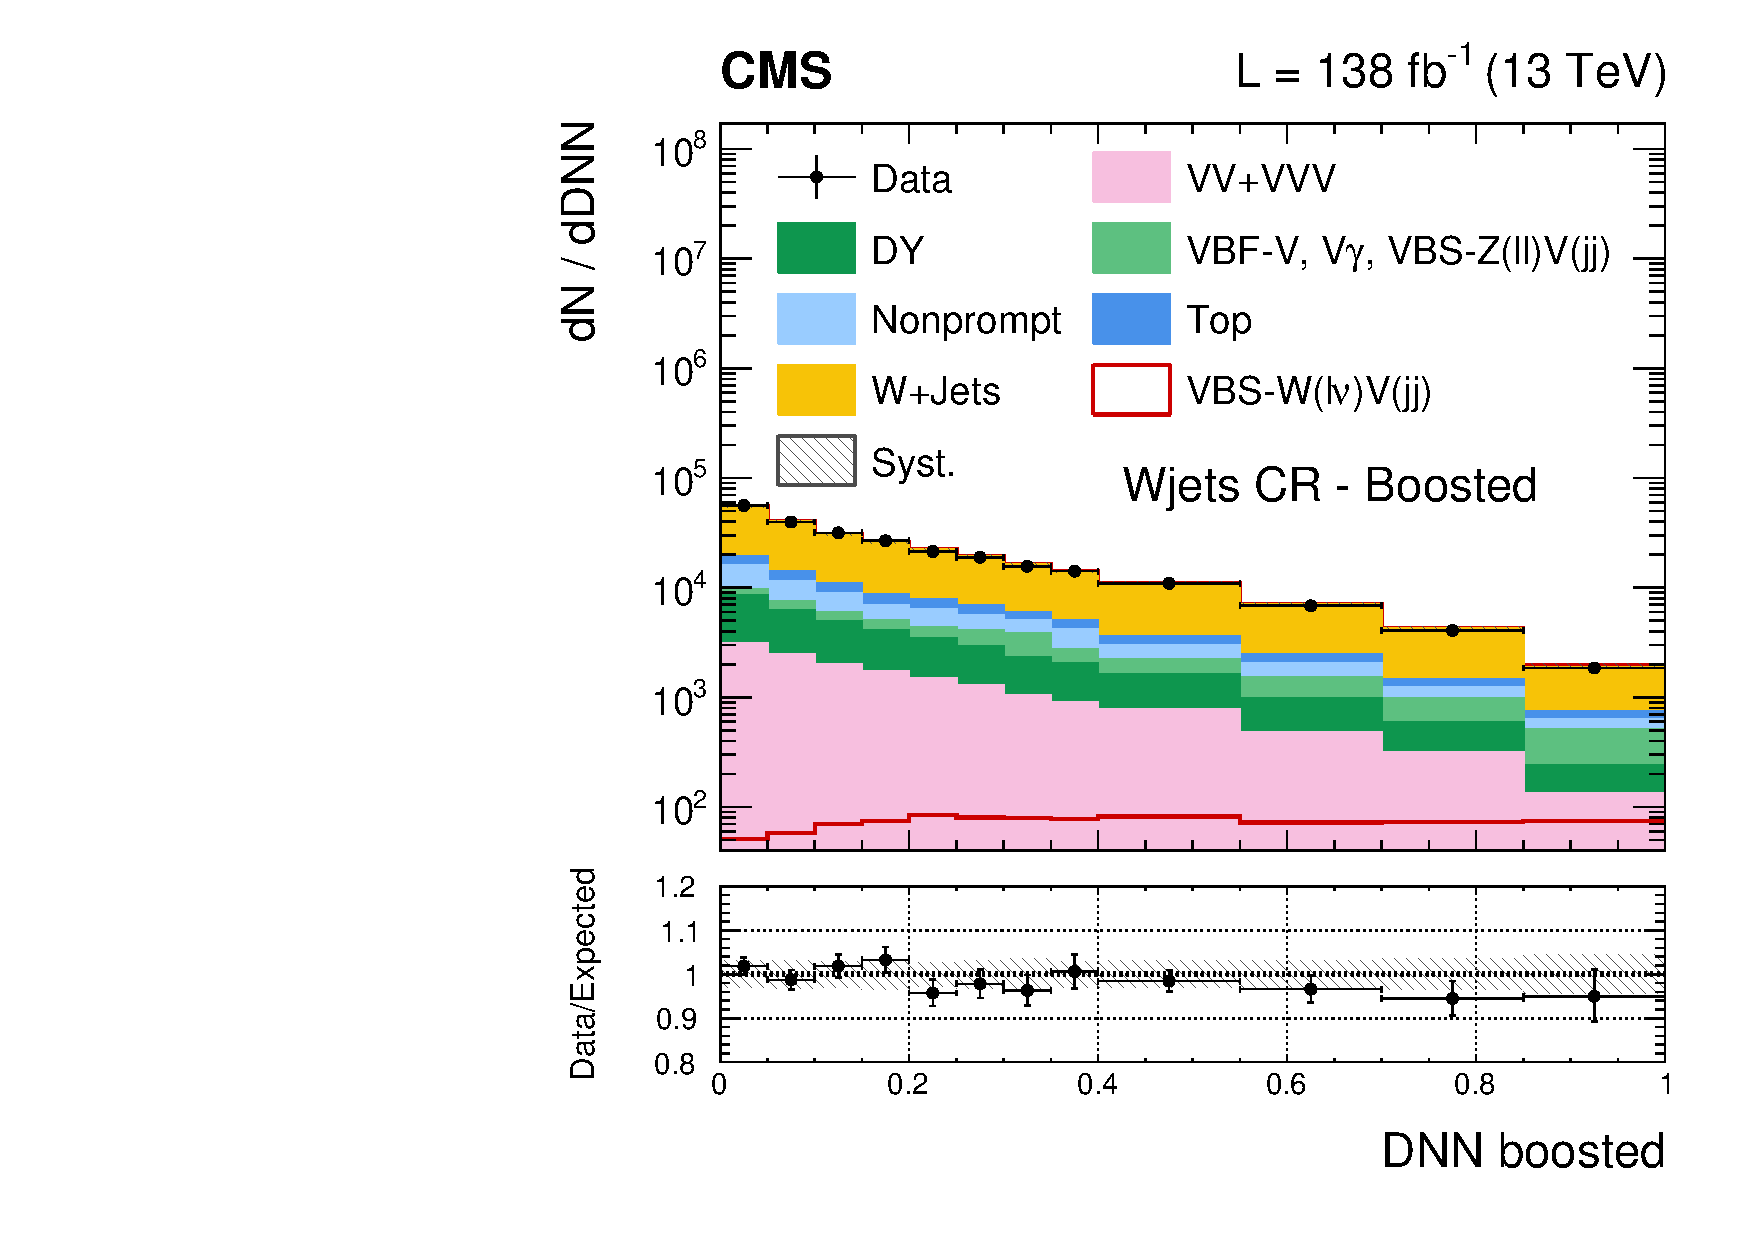
\includegraphics[width=0.49\textwidth]{Images/VBS_Studies/Figure_004-d.pdf}
  \caption{
    The DNN discriminator distribution for the resolved (left) and boosted (right) phase space region in the top quark
    (upper plots) and {\PW}+jets (lower plots) control regions.  Vertical bars on data points show the statistical
    error, whereas the gray band is the post-fit uncertainty on MC with all systematic uncertainties included.
    } \label{fig:CR:dnn}
\end{figure*}


The target of this analysis is the extraction of the $\PW\PV$ VBS production signal strength and the corresponding
significance, obtained through a modified frequentist approach based on the ratio of the experimental likelihood
profiled along with the measurement nuisance parameters over the global likelihood maximum~\cite{Cowan:2010js}.
The likelihood function is built on a signal model taken from simulation and corrected for all residual data/MC
disagreements in particle reconstruction, selection efficiency, and on background models that are built based on
estimates from control samples in data or corrected for data-to-simulation disagreements, as needed.  The DNN
distributions are fitted in the signal phase space regions, combining the two different light lepton flavors, whereas
the yields in the control regions are used only to normalize the {\PW}+jets and top quark backgrounds.


\section{Systematic uncertainties}\label{sec:7}

In the signal extraction fit, each uncertainty is represented by a nuisance parameter that changes the shapes of the
distributions for the signal and background processes or scales their total normalization.  Different sources of
uncertainty are treated as completely uncorrelated in the fit, whereas each uncertainty effect is treated as correlated
or uncorrelated between different channels and processes depending on the case.
In Table~\ref{tab:uncertainty_breakdown} the uncertainties are split into various categories by evaluating the effect on
the total signal strength of freezing each component independently in the fit.

The integrated luminosities of the 2016, 2017, and 2018 data-taking periods are individually known with uncertainties in
the 1.2--2.5\%
range~\cite{CMS-LUM-17-003,CMS-PAS-LUM-17-004,CMS-PAS-LUM-18-002},
whereas the total Run~2 (2016--2018)
integrated luminosity has an uncertainty of 1.6\%.  The improvement in precision reflects the (uncorrelated) time
evolution of some systematic effects.

Discrepancies in the lepton reconstruction and identification efficiencies between data and MC simulation are
compensated by applying correction factors to all samples as functions of the lepton \pt and $\eta$.  Their impact on
the signal region is less than 1\% for both electrons and muons.  The trigger efficiency uncertainty is also smaller
than 1\%.  The electron and muon momentum scale uncertainties are computed by varying the lepton momenta within their
$\pm 1\sigma$ uncertainty, and the resulting uncertainty in the signal yield is less than 1\%. Similarly, jet energy
scale and resolution uncertainties are evaluated by shifting the \pt value of the jets, and thus directly affecting the
reconstructed jet multiplicity and \ptmiss measurement \cite{Khachatryan:2016kdb}; several independent sources are
considered and partially correlated among different data sets, resulting in up to 4\% uncertainty in the signal
strength.

The {\PQb}-tagging data/MC corrections are associated with different uncertainty sources and correlated among all
processes.  Since these uncertainties migrate events between the signal region and top quark control region, they have a
large effect, 5\%, on the signal and background.  Uncertainty in the \ptmiss estimation due to unclustered energy is
also included and calculated by varying the momenta of particles that are not identified with either a jet or a lepton;
its effect is negligible.  Finally, the uncertainty in the pileup modeling is applied to all the relevant MC samples by
varying the minimum bias cross section used to generate the pileup distribution by $\pm 1\sigma$ \cite{CMS:2018mlc} and
estimated to be less than 1\%.

The uncertainty due to the finite number of events in the fitted templates has a significant impact, 10\%, on the signal
measurement. This contribution is dominated by the uncertainty in the nonprompt template estimation, given by the
limited number of data events in the tails and by the large variation of the (positive and negative) weights applied to
model the lepton misidentification probability. Leaving the normalization of the top quark and W+jets (split into many
subcategories) backgrounds floating in the fit results in an uncertainty in the signal strength of 8\%.


The most important theoretical uncertainty is related to the choice of the renormalization and factorization scales in
the MC simulation of events.  The uncertainty in the signal and background yields is computed by taking the largest
variation given by changing such scales up and down independently by a factor of two with respect to their nominal
value, ignoring the extreme case where they are shifted in opposite directions \cite{Cacciari:2003fi,Catani:2003zt}.
The theoretical scale uncertainty is uncorrelated for each background and signal process.  Only shape effects are
included by varying the scales for {\PW}+jets and top quark backgrounds, since their normalization is directly measured
from data in the fit.  Both the shape and normalization effects are included for the other backgrounds.  For the signal,
only the shape effect of the theoretical scales uncertainty is considered while measuring the signal cross section and
significance, whereas the normalization effect is included for the signal strength determination.  Inclusively, the
theoretical scale uncertainty for the EW-only $\PW\PV$ signal is 5\%, and for the QCD-associated diboson production is
25\%.  The overall impact on the EW-only signal strength determination from the choice of renormalization and
factorization scales is 11\%.

The uncertainty in the modeling of the parton shower is also included, by using the weights corresponding to variations
of $\alpS^{\mathrm{ISR}}$ and $\alpS^{\mathrm{FSR}}$ computed by the parton shower programs, and uncorrelated for each
process: the impact on the signal strength determination is 4\%.  The PDF and related strong coupling {\alpS}
uncertainties are evaluated using the eigenvalues of the PDF set following the NNPDF prescription~\cite{Rojo:2016ymp}.
These uncertainties, as well as the one from the modeling of the underlying event, are included for all the processes
apart from top quark and {\PW}+jets backgrounds, and they have a negligible impact on the signal measurement.


\begin{table}[!htb]
  \caption{Breakdown of the uncertainties in the EW $\PW\PV$ VBS signal strength
  measurement.}
  \label{tab:uncertainty_breakdown}
  \centering
  \begin{tabular}{ l c }
  Uncertainty source & $\Delta \mu_{\mathrm{EW}}$ \\
  \hline
  Statistical & 0.12\\
  Limited sample size & 0.10 \\
  Normalization of backgrounds   & 0.08 \\
  Experimental & \\
  \hspace{2em}  {\PQb}-tagging & 0.05 \\
  \hspace{2em}  Jet energy scale and resolution &  0.04 \\
  \hspace{2em} Integrated luminosity & 0.01 \\
  \hspace{2em} Lepton identification & 0.01 \\
  \hspace{2em} Boosted {\PV} boson identification & 0.01 \\
  \hspace{2em} Total & 0.06 \\
  Theory & \\
  \hspace{2em} Signal modeling & 0.09 \\
  \hspace{2em} Background modeling & 0.08 \\
  \hspace{2em} Total & 0.12 \\
  \hline {Total} & 0.22 \\
  \end{tabular}
\end{table}



\section{Results} \label{sec:8}
Three separate maximum likelihood fits are performed: (i) the measurement of the purely EW signal strength $\mew$ keeping
the QCD $\PW\PV$ production contribution fixed to the SM prediction $\mqcd=1$; (ii) the measurement of the signal strength
considering as signal the EW and QCD $\PW\PV$ processes together; (iii) a two-dimensional simultaneous measurement of the
signal strengths $\mew$ and $\mqcd$.

Figure~\ref{fig:dnnbin} shows the post-fit DNN distribution for the resolved (left) and the boosted (right) signal phase
space in the EW-only fit. The background-subtracted plot, where the evidence for the signal is clearly visible, is also
shown.

\begin{figure*}[!htb]
  \centering 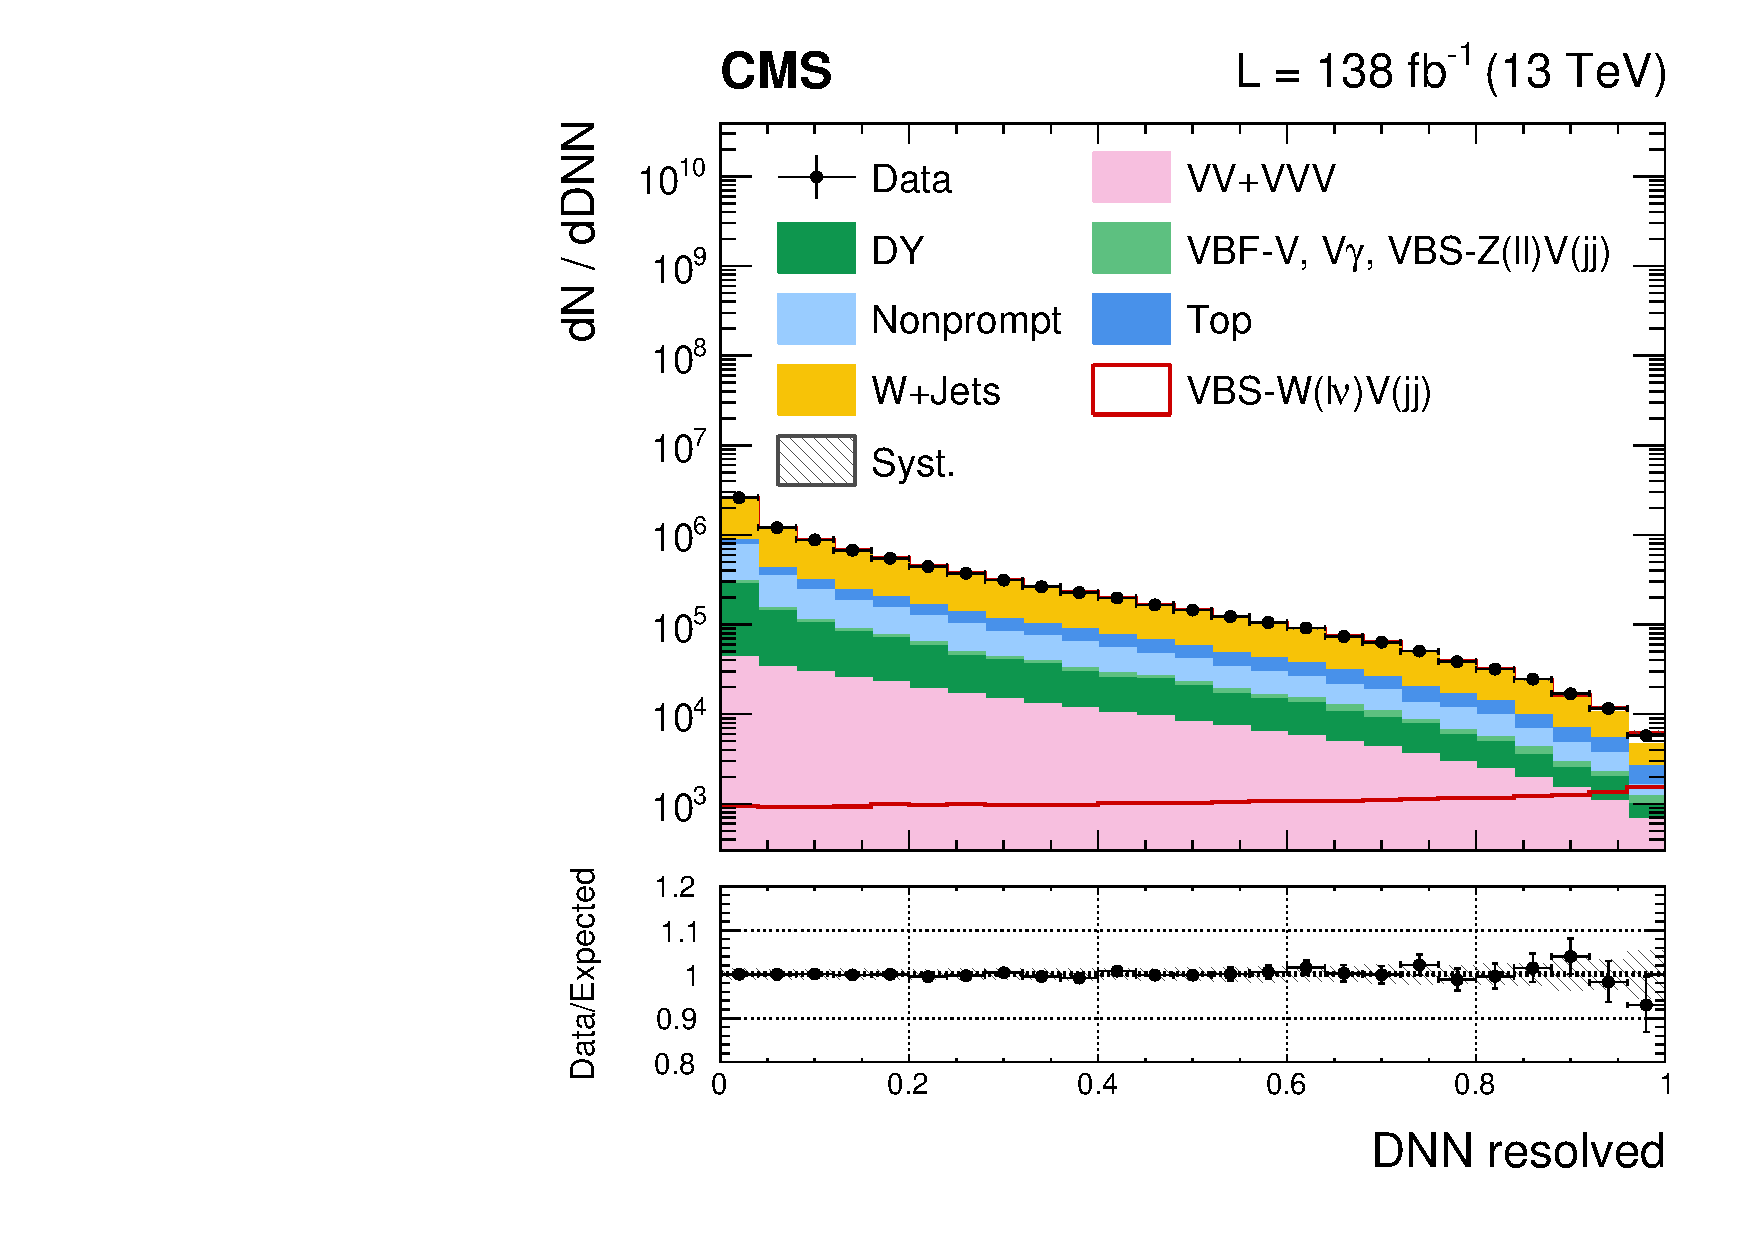
\includegraphics[width=0.49\textwidth]{Images/VBS_Studies/Figure_005-a.pdf} 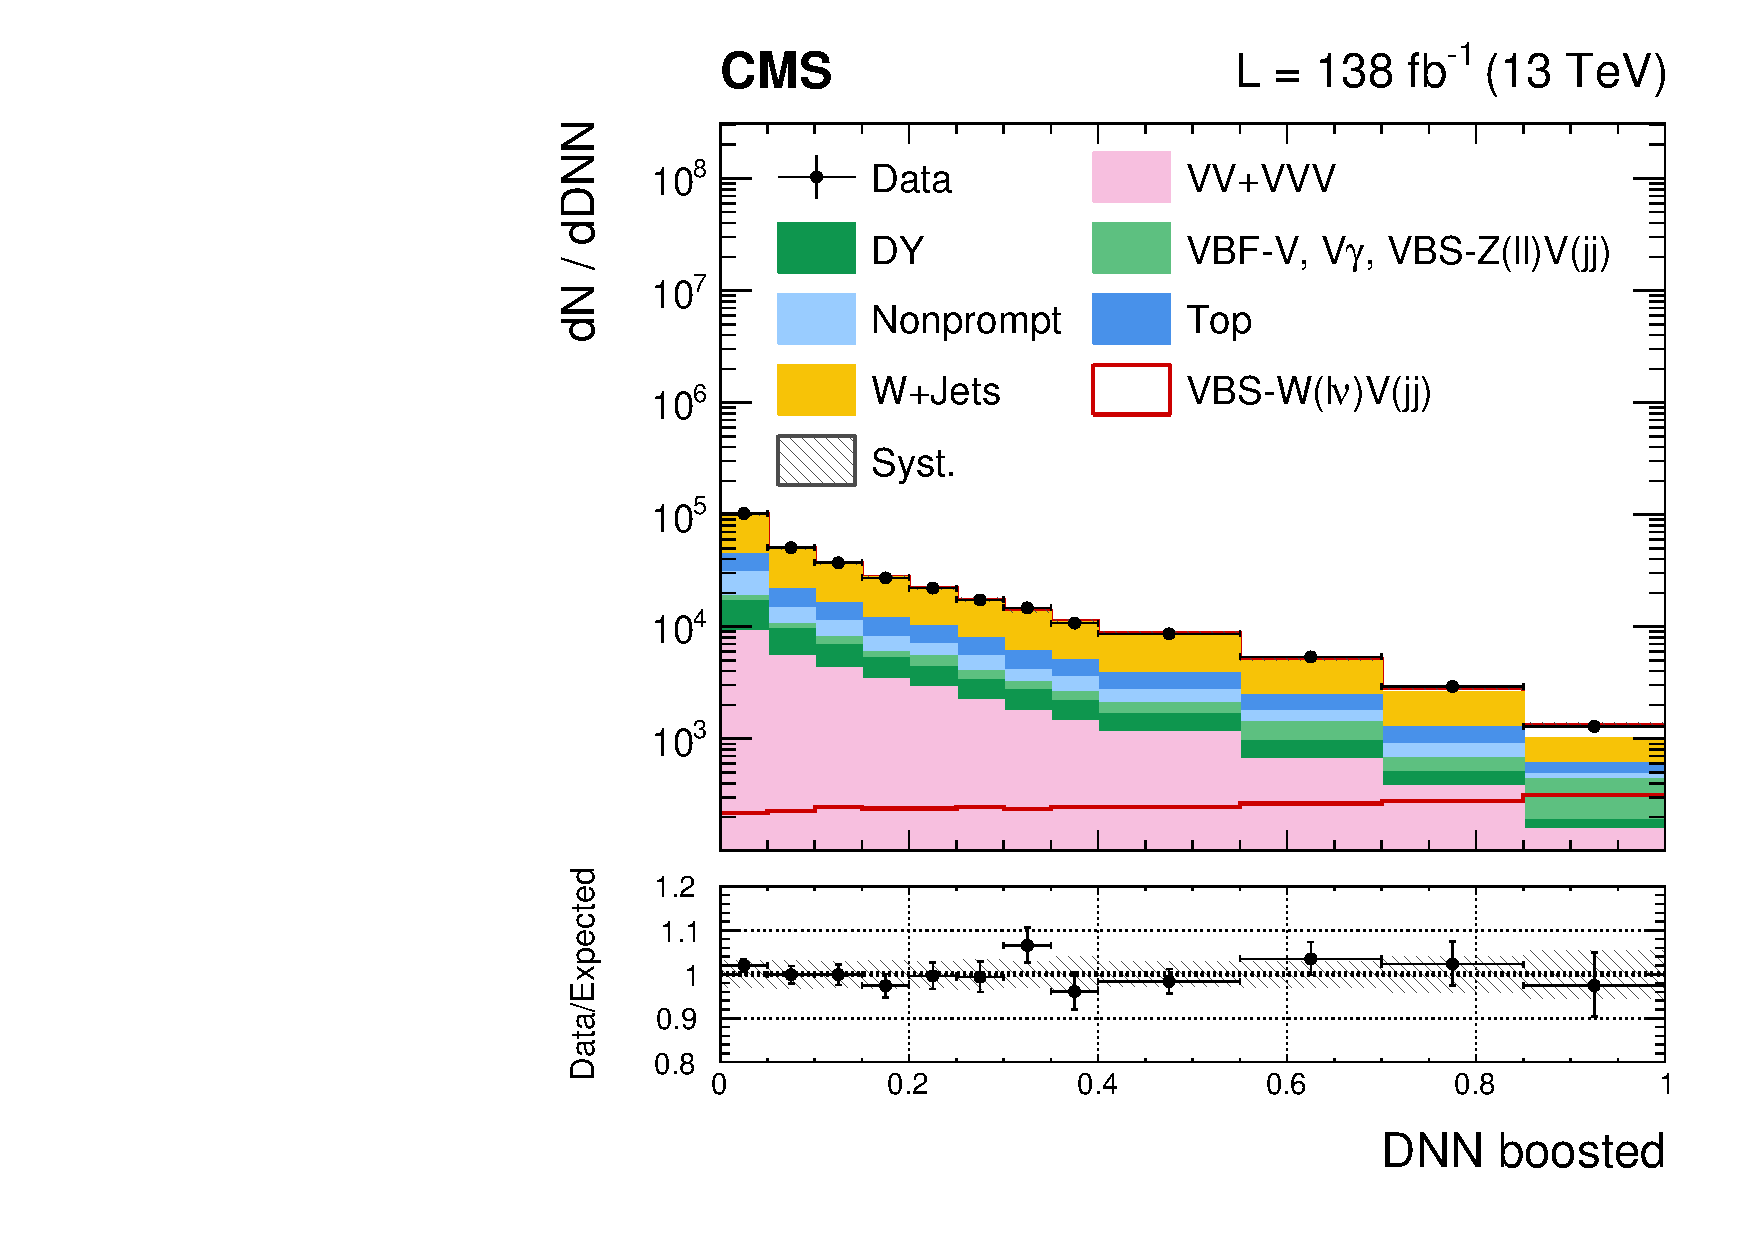
\includegraphics[width=0.49\textwidth]{Images/VBS_Studies/Figure_005-b.pdf} 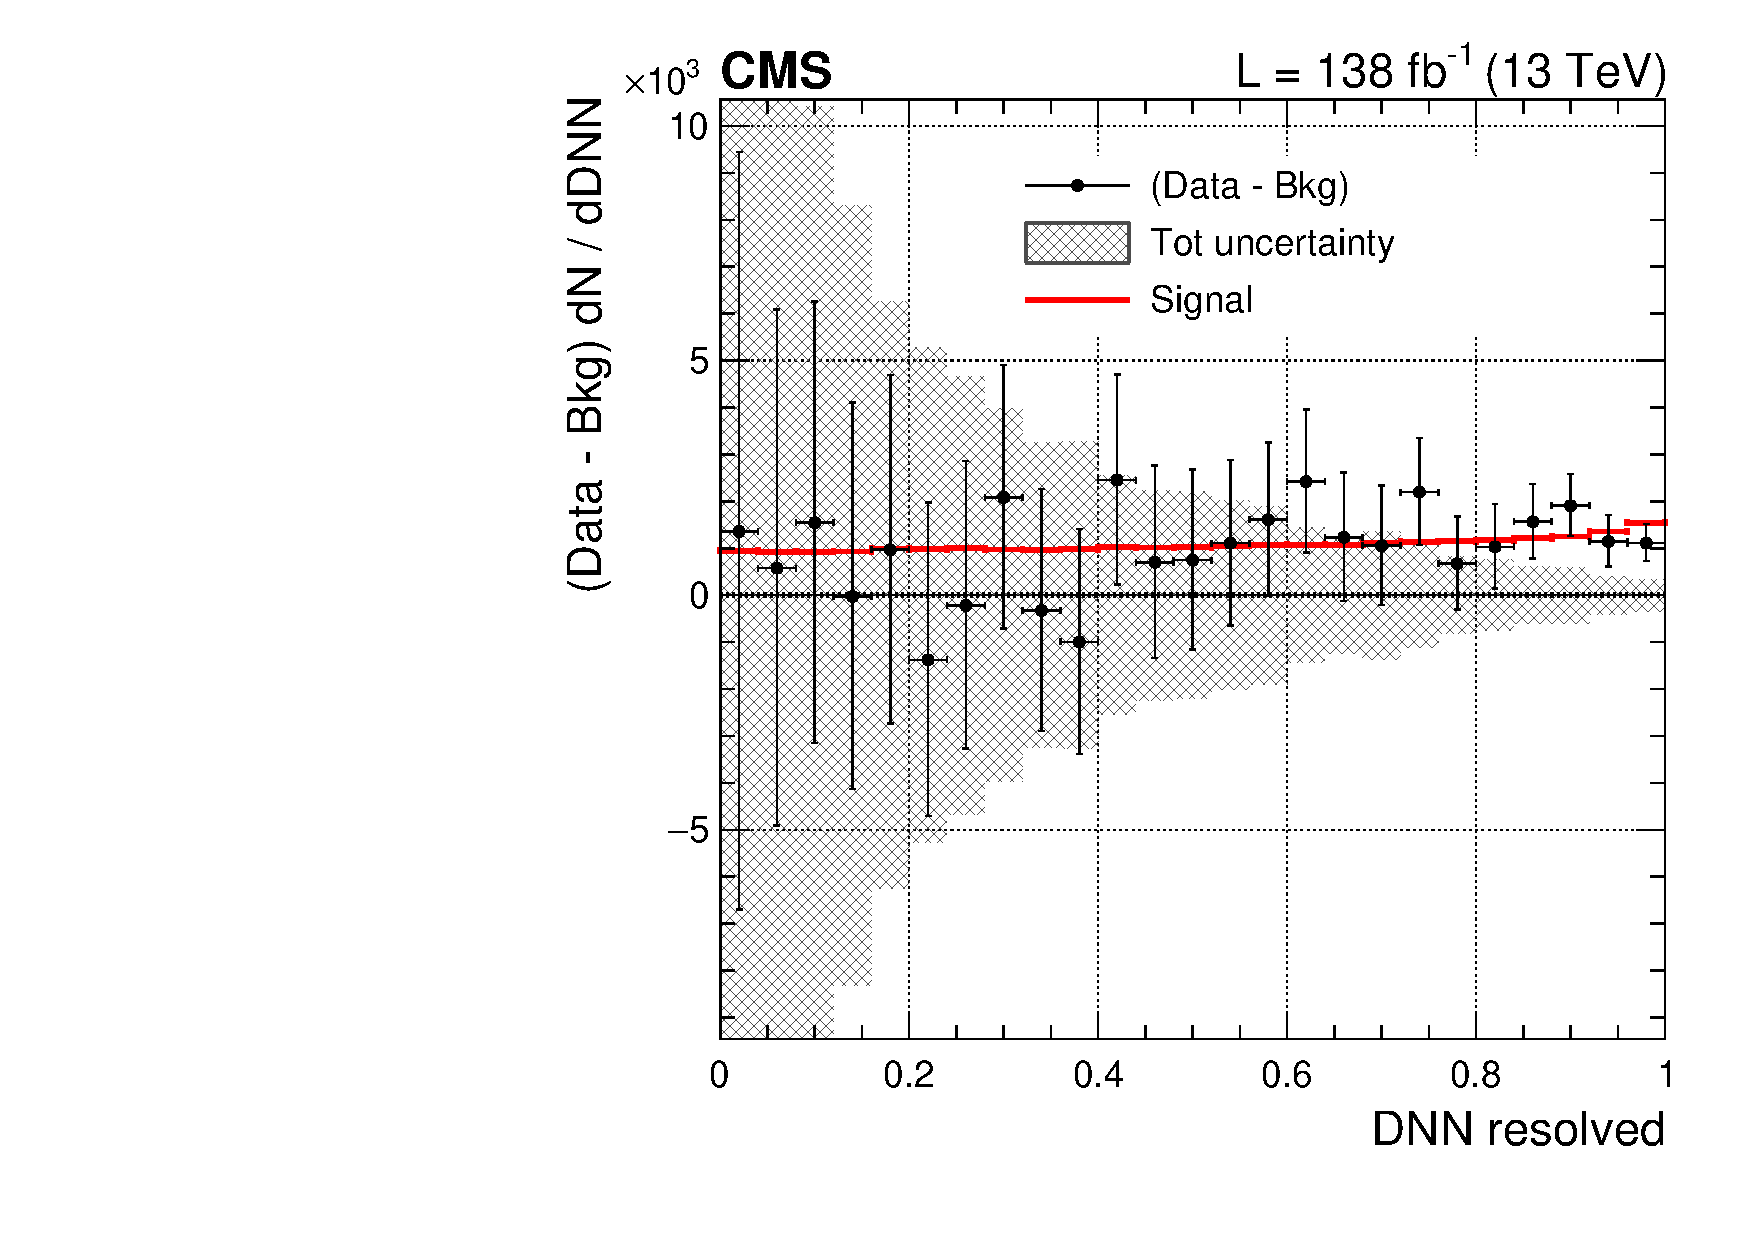
\includegraphics[width=0.49\textwidth]{Images/VBS_Studies/Figure_005-c.pdf} 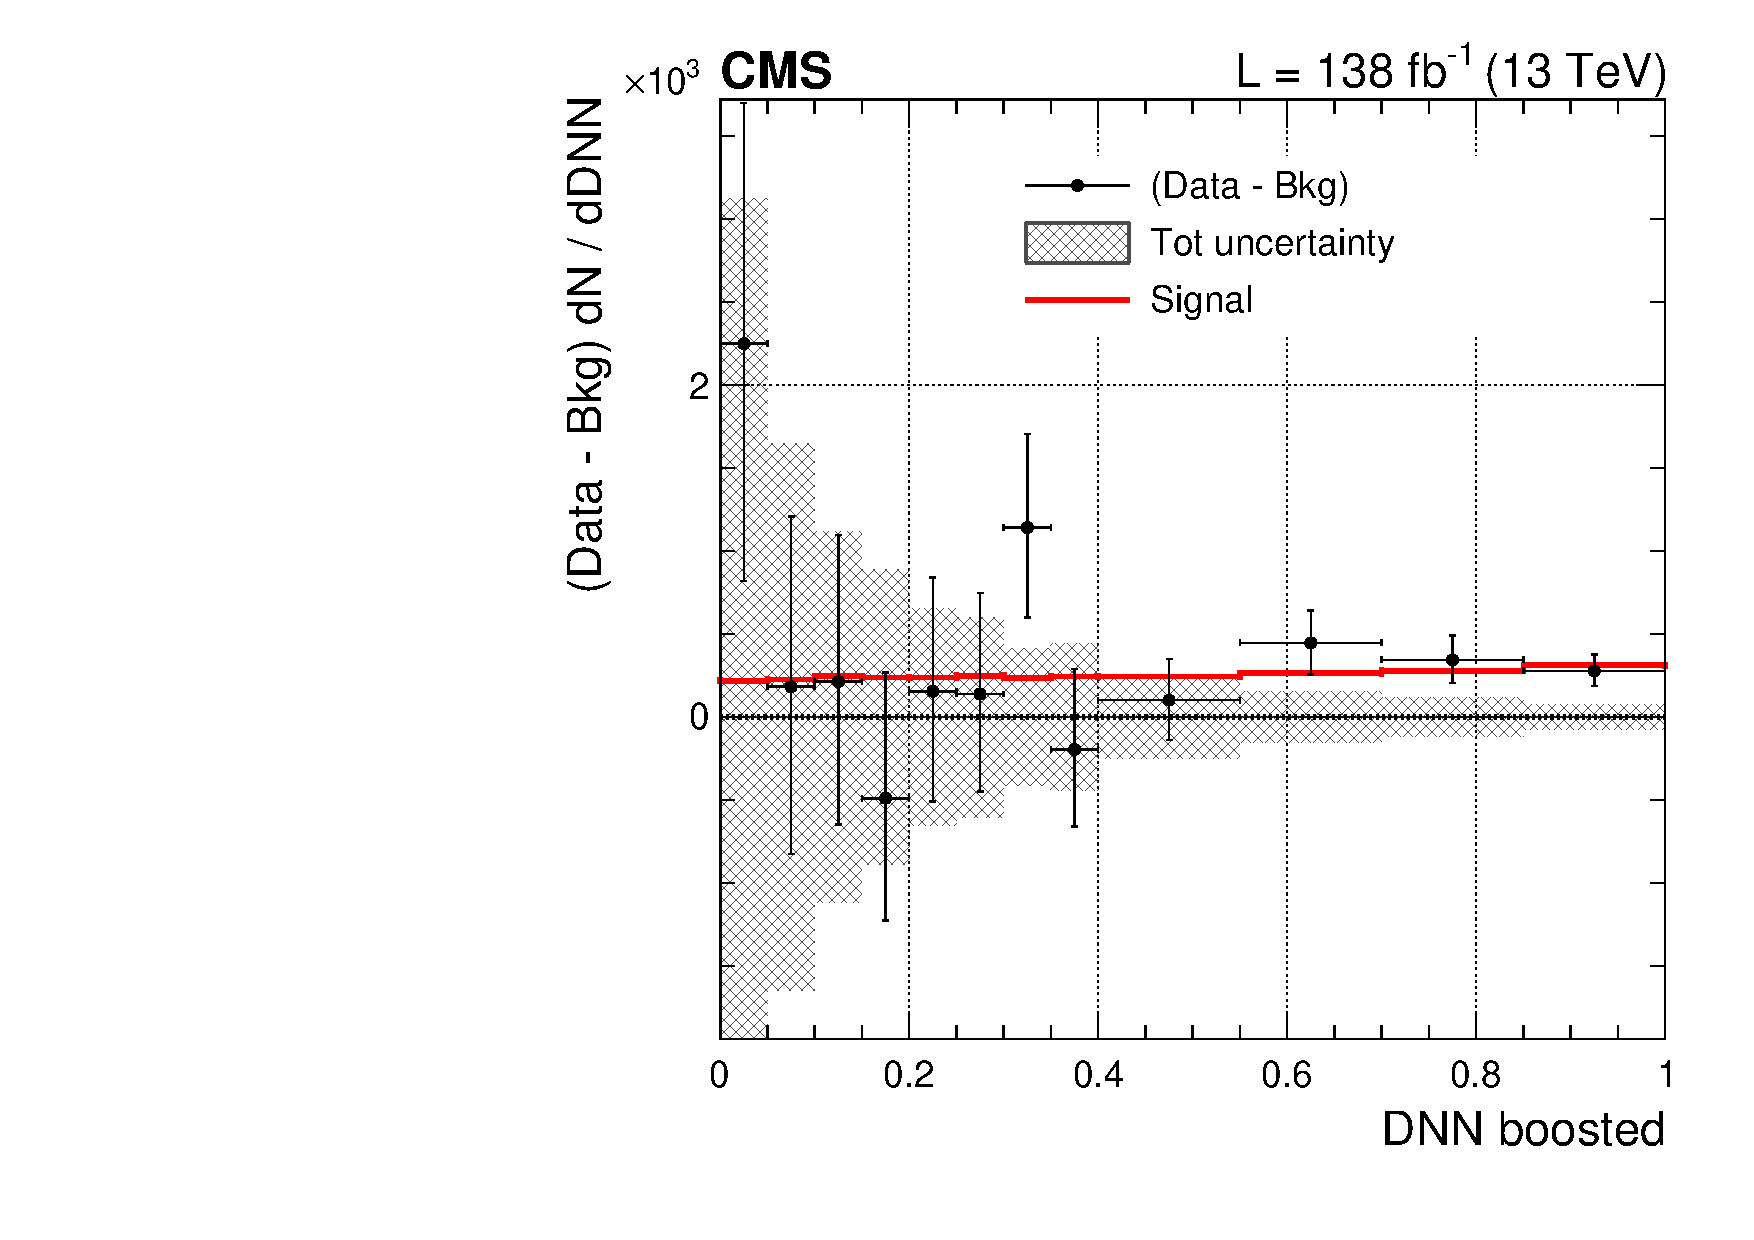
\includegraphics[width=0.49\textwidth]{Images/VBS_Studies/Figure_005-d.pdf} \caption{
    Results for the EW-signal-only fit, keeping the QCD $\PW\PV$ contribution fixed to the SM prediction.  Upper plots:
    post-fit DNN discriminator distributions for the resolved (left) and the boosted (right) signal regions.  The signal
    contribution is plotted both stacked on top of the background processes and also overlaid as a red line to show the signal postfit
    distribution. The expected yield is the sum of signal and background.  Lower plots: background-subtracted DNN
    discriminator distribution for the resolved (left) and the boosted (right) categories. Post-fit background yields in
    each bin are subtracted from data and compared with the signal post-fit distribution, plotted as a red line.
    Vertical bars on data points show the statistical error, whereas the gray band is the post-fit uncertainty on MC
    with all systematic uncertainties included.  } \label{fig:dnnbin}
\end{figure*}

A fiducial phase space region is defined at parton level requiring all partons to have $\pt > 10\GeV$ and at least one
pair of outgoing partons with invariant mass $m_{\PQq\PQq}>100\GeV$.  This simple definition of the fiducial region is
chosen for easy application to signal models; the signal is expected to account for about one quarter of the events in
this region.

The SM prediction for the EW $\PW\PV$ production
cross section in this fiducial region is $2.23^{+0.08}_{-0.11}\,(\text{scale}) \pm0.05\,(\text{PDF})$\unit{pb}, where
PDF refers to the uncertainty coming from the parton distribution function.  The measured EW WV production cross section is
$1.90^{+0.53}_{-0.46}$\unit{pb}, corresponding to an observed EW-only signal strength of:
\begin{linenomath}
\begin{equation}
\mew = \frac{\sobs}{\ssm} =  0.85\pm0.12\,(\text{stat})^{+0.19}_{-0.17}\,(\text{syst}) =0.85 ^{+0.23}_{-0.21},
\end{equation}
\end{linenomath}
where \sobs and \ssm are the observed and predicted cross sections, respectively, with an expectation of
$1.00^{+0.24}_{-0.22}$.  The observed significance for the SM EW $\PW\PV$ signal is 4.4 standard deviations with 5.1
expected. The EW-only signal strength fitted independently in the resolved and boosted categories is $0.85\pm0.26$ and
$1.09\pm0.32$, respectively.

Considering instead the signal as the overall EW and QCD-associated diboson production, the measured and expected cross
sections are $16.4^{+3.5}_{-2.8}$\unit{pb} and $16.9^{+2.9}_{-2.1}\,(\text{scale}) \pm0.5\,(\text{PDF})$, respectively,
extracted in the same fiducial phase space region as the EW-only one. This fit assumes the ratio between the EW and
QCD contributions to the diboson production is fixed to the value predicted by the SM.  The overall signal strength
$\mu = \sobs / \ssm$, with an expectation of $1.00^{+0.21}_{-0.20}$, is measured as:
\begin{linenomath}
\begin{equation}
\mu_{\mathrm{EW}+\mathrm{QCD}} =  0.97\pm0.06\,(\text{stat})^{+0.19}_{-0.21}\,(\text{syst})= 0.97 ^{+0.20}_{-0.22} ,
\end{equation}
\end{linenomath}
The fit is also performed leaving as free independent parameters the signal strengths of the EW and QCD-associated
$\PW\PV$ production components ($\mew$ and $\mqcd$).  The result of the 2D fit is shown in Fig.~\ref{fig:fit_2d}, where
the expected and observed minima are presented, together with the 68 and 95\% confidence level (\CL) contours built from
the likelihood function.  The measured signal strengths are in agreement with the SM predictions within the 68\% \CL.

\begin{figure}[!htb]
  \centering 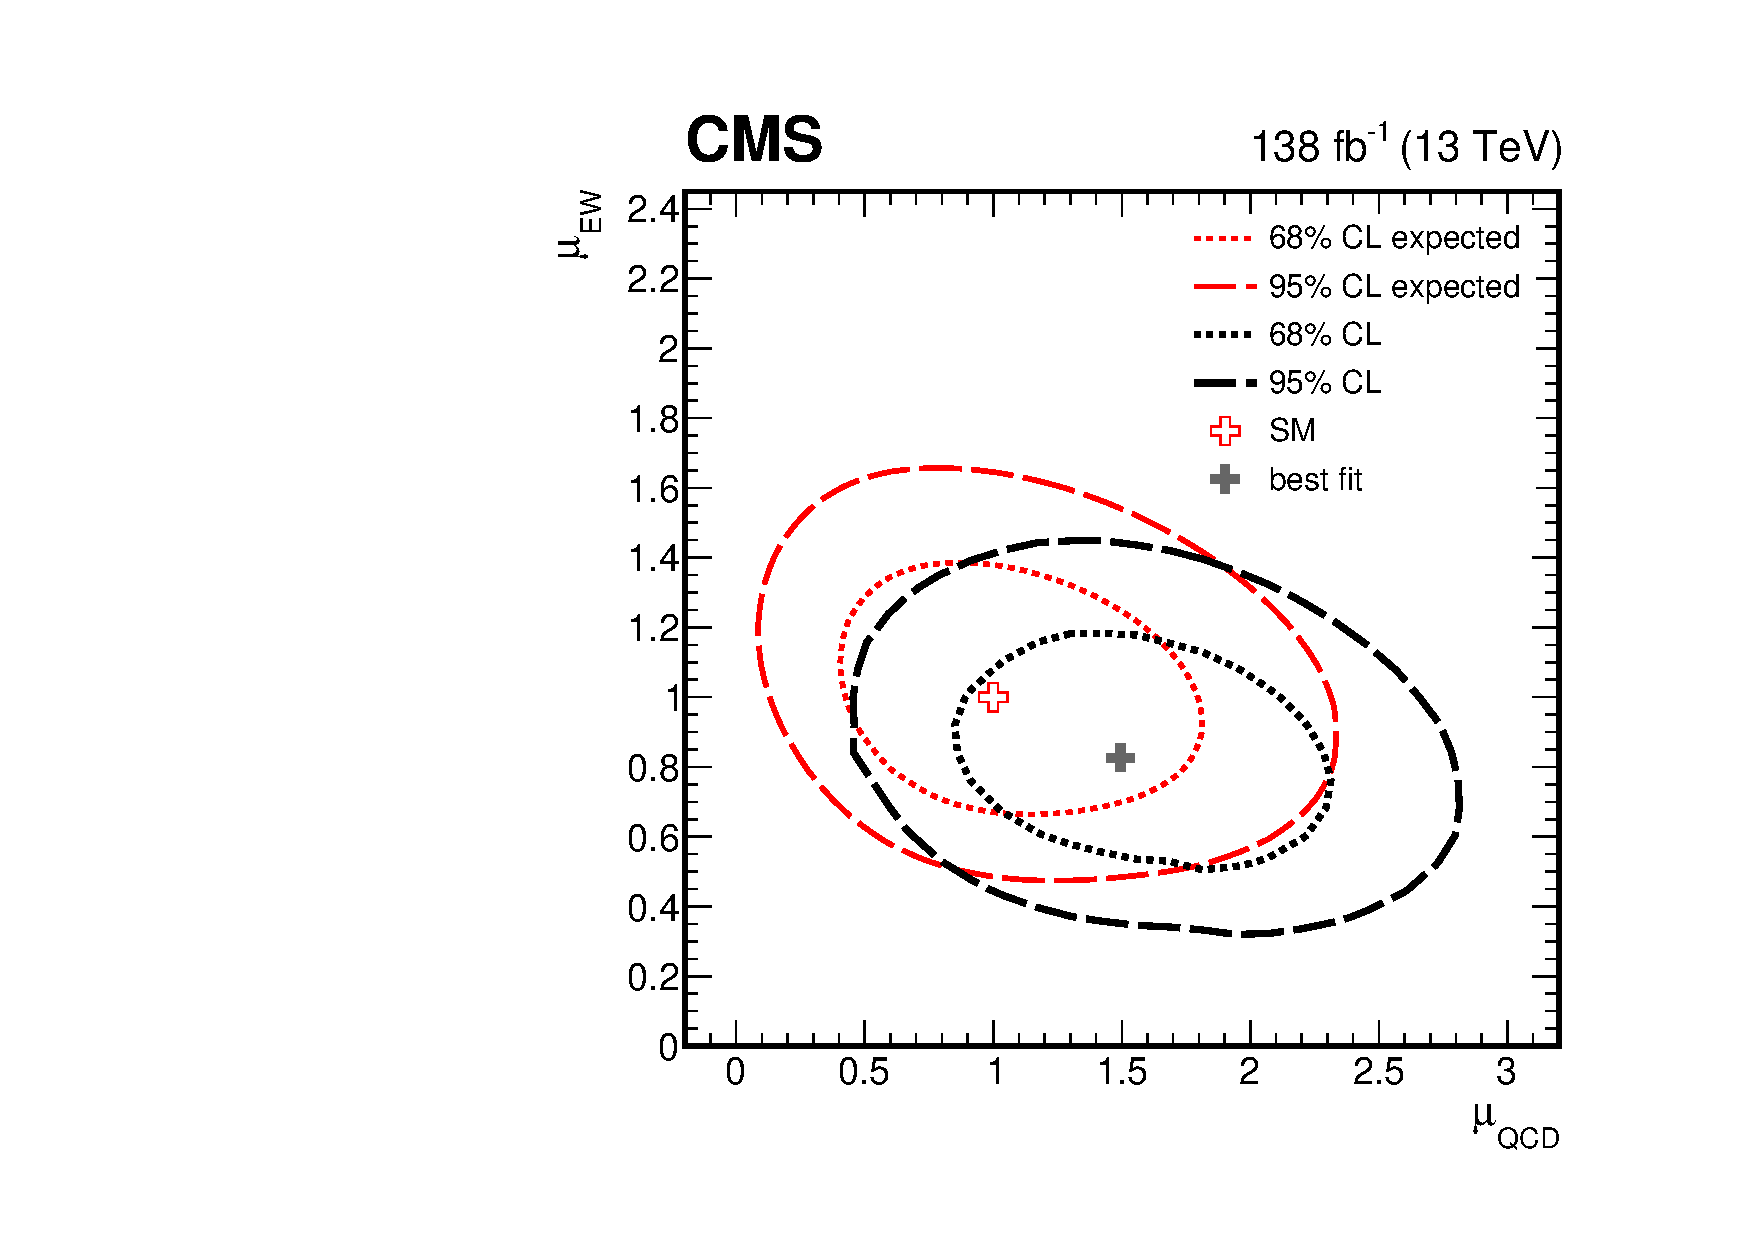
\includegraphics[width=0.5\textwidth]{Images/VBS_Studies/Figure_006.pdf} \caption{Simultaneous EW and QCD $\PW\PV$ production
    fit: the expected and observed 68 and 95\% \CL contours on the signal strengths. The best fit result is compatible
    with the SM prediction within the 68\% \CL area.  } \label{fig:fit_2d}
\end{figure}


\section{Summary}\label{sec:9}

The first evidence for the electroweak (EW) production of a $\PW\PV$ ($\PV = \PW$ or {\PZ}) pair plus two jets in the
$\ell\nu\PQq\PQq$ decay channel is reported.  Events are separated into two categories: either the hadronically decaying
{\PW} or {\PZ} boson is reconstructed as one large-radius jet, or it is identified as a pair of jets with dijet mass
close to the boson mass.  Multivariate machine learning discriminators are optimized to separate the signal from the
background in each category and their outputs are exploited in the statistical analysis.  The large background from
single {\PW} boson production accompanied by jets is estimated from control samples in the data to reduce the impact of
Monte Carlo mismodeling in this multijet phase space region.

Tabulated results are provided in the HEPData record for this analysis~\cite{HEPData_SMP-20-013}.

The measured EW-only $\PW\PV$ signal strength is:
$\mew = \sobs / \ssm = 0.85\pm0.12\,(\text{stat})^{+0.19}_{-0.17}\,(\text{syst}) = 0.85 ^{+0.23}_{-0.21} $
at $1.00^{+0.24}_{-0.22}$ expected, where \sobs and \ssm are the observed and predicted cross sections, respectively.
The observed significance for the SM EW $\PW\PV$ signal is 4.4 standard deviations with 5.1 expected.
When we consider the signal as the total EW and QCD-associated diboson yield, the overall signal strength
$\mu_{\mathrm{EW}+\mathrm{QCD}}$ is measured as: $0.97\pm0.06\,(\text{stat})^{+0.19}_{-0.21}\,(\text{syst}) = 0.97
^{+0.20}_{-0.22}$ with an expectation of $1.00^{+0.21}_{-0.20}$.  Finally, a simultaneous two-dimensional fit of the EW
and QCD $\PW\PV$ production components is performed.

Overall, both the $\PW\PV$ EW-only measurement and the simultaneous EW and QCD $\PW\PV$ measurements are in agreement
with the SM predictions within the 68\% confidence level.


\chapter{Non-resonant HH production} \label{Chapter:HH_NonResonant}

\section{Introduction}\label{section:introduction_HH}
Since the experimental discovery of a particle consistent with the standard model (SM) Higgs boson by the CMS and ATLAS experiments at the CERN 
LHC in 2012 \cite{Aad:2012tfa,Chatrchyan:2012ufa,Chatrchyan:2013lba}, physicists
have sought to further their understanding of the Higgs boson and the underlying electroweak symmetry breaking process. Additionally, the Higgs boson
has been widely explored as a potential bridge to physics beyond the standard model (BSM).

Through the investigation of Higgs pair production, the production of two Higgs bosons in a single process, physicists can both test SM predictions and 
search for BSM. On the SM front, investigating Higgs pair production allows for a fundamental test as the shape of the Higgs potential in the SM Lagrangian 
depends on the Higgs self-coupling value, which can be directly accessed via Higgs pair production. A precise measurement of this coupling would provide the first experimental insight 
into the shape of the Higgs potential, which can have profound implications on the understanding of our world, for example by providing evidence that the Higgs vaccum expectation value sits at a 
meta-stable minimum consistent with the SM prediction. Alternatively, a measurement which is not consistent with this SM prediction could hint to physics beyond the standard model \cite{10.3389/fspas.2018.00040}. 

The main leading order (LO) processes which contribute to the cross section of Higgs pair production in the gluon fusion production mode ($gg \to HH$) are the ``triangle'' and ``box'' diagrams, shown in Fig. \ref{SMLO_ggHH_production}. 
The box diagram is sensitive to the top Yukawa coupling, while the triangle diagram is sensitive to both the top Yukawa and trilinear self-coupling. 
Hence, the resulting cross-section is particularly sensitive to these parameters, whose values are precisely predicted in the SM. Assuming a self-coupling strength as predicted
by the SM, these diagrams destructively 
interfere, leading to a small production cross section. In order to search for this relatively small signal, a search is performed in the WW$\gamma\gamma$ channel. 
This final state benefits from the sensitive $H\rightarrow\gamma\gamma$ process which provides a narrow, distinguishable signature. Additionally, the
$H\rightarrow WW$ leg of the decay contributes a relatively large branching ratio among Higgs boson decays of about 22\%. 
Because the W boson can decay both leptonically and hadronically, the $H\rightarrow WW$ and by extension the $HH\rightarrow WW\gamma\gamma$ process has three possible final states:
The fully-hadronic (FH), semi-leptonic (SL), and fully-leptonic (FL) final states, corresponding to 0, 1, and 2 leptonically decaying W-bosons respectively. These three final states can be identified in data and simulation
with separate selections and categorizations, and their corresponding
signal and background models can be simultaneously fit to data in order to improve the overall analysis sensitivity. Due to the expected overlap between the FH WW$\gamma\gamma$, FH ZZ$\gamma\gamma$, and bb$\gamma\gamma$ di-Higgs
final states, the FH ZZ$\gamma\gamma$ and bb$\gamma\gamma$ final states are also considered as signal in the analysis.

In addition, several BSM models predict the existence of real and virtual heavy particles that can couple to a pair of Higgs bosons \cite{deFlorian:2016spz, Nakamura:2017irk, Englert:2019eyl, Robens:2019kga, Tang:2012pv}.
These can lead to the appearance of a resonant contribution to the invariant mass of the $HH$ system, or to a significant modification of Higgs boson pair production through virtual processes. Assuming that any new particle has a 
mass too large to be created at the LHC, we can parameterize 
these possible effects at LHC energy scales using an Effective field theory (EFT) approach ~\cite{deFlorian:2016spz, Carvalho:2015ttv}. The effects are parametrized either as modifications to the SM couplings, 
or as contact interactions. In the SM coupling modifications, possible new resonances contribute through loop diagrams whereas the contact interaction is a way of 
describing a process where the mediator has a mass far above the momentum transfer in the event and therefore can be both via a triangular virtual loop or resonant production. 
The interpretations of this analysis include the purely SM interpretation, an EFT interpretation leading to scans of modified SM and purely BSM lagrangian coupling constants, 
and a search for 20 EFT benchmarks corresponding to points largely representative of the 5-dimensional EFT phase space \cite{Carvalho:2015ttv,Buchalla:2018yce,Capozi:2019xsi}.  

This is the first search for Higgs pair production in the WW$\gamma\gamma$ final state performed by the CMS experiment, and is performed using pp collisions at $\sqrt{s} = $ 13 TeV.
The data sample corresponds to an integrated luminosity of 138 \unit{fb}$^{-1}$ collected with the CMS detector at the CERN LHC during Run 2 (2016-18).
A search in the SL WW$\gamma\gamma$ final state was performed 
by the ATLAS experiment using data collected at the LHC in 2016, where a cut-based analysis was performed to obtain an observed (expected) upper limit on SM di-Higgs
production of 7.7 (5.4) pb at a 95\% confidence level \cite{Aaboud2018}. 

The structure of this chapter is as follows: A description of the EFT parameterization and
benchmarks is provided in Section \ref{sec:EFT_Description}. The data samples and simulated events are described in Section \ref{sec:samples}. 
The reconstruction of particles as detector objects is described in Section \ref{sec:Objects}. Event selection criteria are described in Section \ref{sec:event_selection}. 
%Further analysis techniques employed in the SL and FH final states is described in Section \ref{sec:AnalysisStrategy}. 
The method of signal and background modelling using simulation and data is
described in Section \ref{sec:AnalyticFitting}. A description of the systematic uncertainties of the analysis is presented in Section \ref{section:Systematics}.
The results of the analysis are described in Section \ref{sec:results}, and a summary is provided in Section \ref{section:Summary}. 

	\section{EFT description} \label{sec:EFT_Description}

The Higgs potential, before spontaneous symmetry breaking, reads: 

\begin{eqnarray}
  V(\Phi) = - \frac{\mu^2}{2}\left|\Phi \right|^2
  +\frac{\lambda}{4} \left|\Phi \right|^4
  \label{eqm-1}
\end{eqnarray}
where $\Phi$ is the $SU(2)$ doublet scalar field and $\phi = v + H$ is the real part of the neutral component ($v$ being its vacuum expectation value).
The condition of a minimum of the potential leads to the relations:
\begin{eqnarray}
  \lambda = \frac{m_H^2}{2 v^2}, \;\;  \mu^2 = \frac{m_H^2}{2},
  \;\; m_H^2 = \frac{\partial^2 V}{\partial \phi^2}
   \label{eqm-2}
\end{eqnarray}

Therefore, in the SM, the Higgs self-coupling is uniquely determined by the structure of the scalar potential (\ref{eqm-1}), which takes the following
form in terms of the physical $H$ field:

\begin{eqnarray}
  V &=& \frac{m_H^2}{2}H^2 + \lambda_3 v H^3 + \frac{\lambda_4}{4} H^4,
\quad
 \lambda_3 = \lambda_4 = \lambda_{HHH} = \frac{m_H^2}{2v^2} \label{eqm-3}
\end{eqnarray}

However, the sign and value of the parameters $\mu^2$ and $\lambda_{HHH}$ in~(\ref{eqm-1}) are a priori arbitrary.
The positive sign of $\lambda_{HHH}$ is necessary for the stability of the potential at large $\phi$.
Moreover, the functional form of (\ref{eqm-1}) is not fundamental: The underlying gauge
symmetry only requires the potential to depend on $\left| \Phi \right|^2$, and the quartic form could simply represent the leading terms in
the power expansion of a more complex functional dependence of the potential (see~\cite{Mangano:2019kji} for detailed considerations).
Thus, experimentally measuring $\lambda_{HHH}$ is a crucial test of the electroweak symmetry breaking mechanism.
In particular, modifications of the Higgs trilinear couplings (e.g. via a modified Higgs self interaction) can only be directly observed in Higgs boson pair production.

We use the following effective Lagrangian~\cite{deFlorian:2016spz, Carvalho:2015ttv} to describe Higgs boson pair production:

\begin{eqnarray}\label{Eq:LagrangianBSM}
&&  \mathcal{L}_{BSM} = -{\textcolor{ForestGreen}{\kappa_{\lambda}}} \lambda^{SM}_{HHH} v H^3 -
  \frac{m_t}{v}({\textcolor{blue}{\kappa_t}} H + \frac{\textcolor{red}{c_2}}{v} H^2)(\bar{t_L}t_R + h.c.)
  +  \frac{\alpha_S}{12 \pi v}(\textcolor{red}{c_g} H
  - \frac{\textcolor{red}{c_{2g}}}{2 v}H^2)G^a_{\mu \nu}G^{a, \, \mu \nu} \\
  && {\textcolor{ForestGreen}{\kappa_{\lambda}}} = \frac{\lambda_{HHH}}{\lambda_{HHH}^{SM}}, \;
  \lambda_{HHH}^{SM} = \frac{ m^2_{H}}{2v^2}, \;\;
  {\textcolor{blue}{\kappa_{t}}} = \frac{ y_{t}}{y_{t}^{SM}}, \;\;
  y_{t}^{SM} = \frac{\sqrt{2} m^2_{t}}{ v}
\end{eqnarray}

\begin{figure}[!htbp]
  \subfloat[SM-like processes]{%
  \label{SMLO_ggHH_production}
            \begin{minipage}[t]{\linewidth}
                  \begin{center}
                          \raisebox{-0.7\height}{ 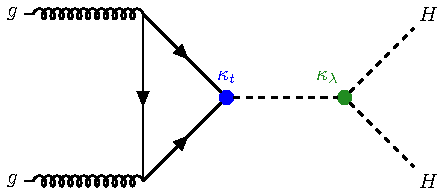
\includegraphics[width=0.45\textwidth]{Images/EFT_Description/fey_HH_Triangle.pdf} }
                          \raisebox{-0.625\height}{ 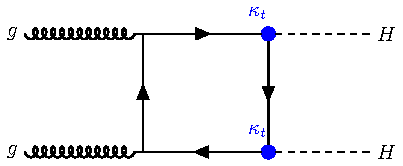
\includegraphics[width=0.45\textwidth]{Images/EFT_Description/fey_HH_Box.pdf} }
                  \end{center} 
          \end{minipage}%
  }
  
  \subfloat[Pure BSM processes]{%
  \label{BSMLO_ggHH_production}
          \begin{minipage}[t]{\linewidth}
                  \begin{center}
                          \raisebox{-0.7\height}{ 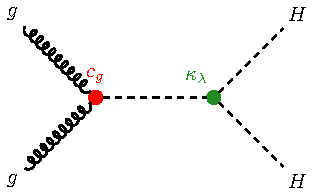
\includegraphics[width=0.30\linewidth,clip]{Images/EFT_Description/fey_HH_anomal_2_colored.pdf} }
                          \raisebox{-0.7\height}{ 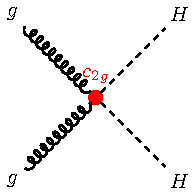
\includegraphics[width=0.20\linewidth,clip]{Images/EFT_Description/fey_HH_anomal_3_colored.pdf} }
                          \raisebox{-0.7\height}{ 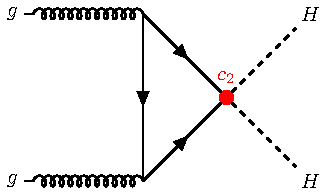
\includegraphics[width=0.30\linewidth,clip]{Images/EFT_Description/fey_HH_anomal_4_colored.pdf} }
                  \end{center}
          \end{minipage}
  }
  \caption{Feynman diagrams for leading-order Higgs boson pair production via gluon fusion}
  \label{fig:ggHH_production}
  \end{figure}
  

where variables are defined as follows:

\begin{itemize} \label{EFT_parameters_description}
  \item $G^a_{\mu \nu} = \partial_{\mu} G_{\nu}^a - \partial_{\nu} G_{\mu}^a + f^{abc}  G_{\mu}^b G_{\nu}^c$ is the gluon field strength tensor
  \item $f^{abc}$ is the totally anti-symmetric $SU(3)$ structure tensor
  \item \textcolor{ForestGreen}{$\kappa_{\lambda}$} - measure of the deviation of the Higgs boson trilinear coupling from its SM expectation $\lambda_{HHH}^{SM}$
  \item \textcolor{blue}{$\kappa_{t}$} - measure of the deviation of the coupling a single Higgs boson and two top quarks from its SM expectation $y_{t}^{SM}$
  \item \textcolor{red}{$c_{2}$} - coupling between two Higgs bosons and two top quarks
  \item \textcolor{red}{$c_{g}$} - coupling between one Higgs bosons and two gluons
  \item \textcolor{red}{$c_{2g}$} - coupling between two Higgs bosons and two gluons
\end{itemize}

The differential cross section of gluon-gluon fusion
induced Higgs boson pair production $\sigma_{HH}$ can be expressed as a polynomial in terms of the
EFT model parameters using generator-level information on the HH system like:

\begin{equation}
\label{eq:rew_3}
  \frac{d^2\sigma}{d m_{HH}d|\cos{\theta^*}| } = \sum A_i( m_{HH}, |\cos{\theta^*}| ) \, c_i
\end{equation}

where the $c_i$ stand for the combinations of couplings as in \cite{Buchalla:2018yce} and $A_i( m_{HH}, |\cos{\theta^*}| )$ are known coefficients.
Eq. (\ref{eq:rew_3}) is used to obtain MC samples corresponding to benchmark samples using a reweighting method \cite{Carvalho:2016rys,Buchalla:2018yce},
where the twenty benchmark scenarios considered in the analysis are shown in Tab. \ref{tab:eft_bench} \cite{Carvalho:2015ttv,Buchalla:2018yce,Capozi:2019xsi}. 

The $\kappa_{\lambda}$ parameter also affects the Higgs boson branching ratios and the single Higgs production cross sections because of next-to-leading (NLO) electroweak corrections \cite{Degrassi:2016wml,Maltoni:2017ims}.

\begin{table}[h]
  \begin{center}
    \begin{tabular}{r|ccccc}
      Benchmark & $\kappa_{\lambda}$ & $\kappa_{t}$ & $c_{2}$	& $c_{g}$ & $c_{2g}$ \\ \hline
      SM &	1.0 & 1.0	 &	0.0		& 0.0	& 0.0 \\ \hline
      1 &	7.5	 & 1.0	 &	-1.0	& 0.0	& 0.0 \\
      2 &	1.0	 & 1.0	 &	0.5		& -0.8	& 0.6 \\
      3 &	1.0	 & 1.0	 &	-1.5	& 0.0	& -0.8 \\
      4 &	-3.5 & 1.5  &	-3.0	& 0.0	& 0.0 \\
      5 &	1.0	 & 1.0	 &	0.0		& 0.8	& -1 \\
      6 &	2.4	 & 1.0	 &	0.0		& 0.2	& -0.2 \\
      7 &	5.0	 & 1.0	 &	0.0		& 0.2	& -0.2 \\
      8 &	15.0 & 1.0	 &	0.0		& -1	& 1 \\
      9 &	1.0	 & 1.0	 &	1.0		& -0.6	& 0.6 \\
      10 &	10.0 & 1.5   &	-1.0	& 0.0	& 0.0 \\
      11 &	2.4	 & 1.0	 &	0.0		& 1		& -1 \\
      12 &	15.0 & 1.0	 &	1.0		& 0.0	& 0.0 \\[0.5ex] \hline 
      8a &  1.0  & 1.0   &  0.5   & $\frac{0.8}{3}$ & 0.0 \\[0.5ex] 
      1b &  3.94 & 0.94  & $\frac{-1}{3}$ & 0.75 & -1 \\[0.5ex] 
      2b &   6.84 & 0.61 &  $\frac{1}{3}$ &  0.0 & 1.0 \\[0.5ex] 
      3b &   2.21 & 1.05 & $\frac{-1}{3}$ &  0.75 &  -1.5 \\[0.5ex] 
      4b &   2.79 & 0.61 &  $\frac{1}{3}$ & -0.75 &  -0.5 \\[0.5ex] 
      5b &   3.95 & 1.17 & $\frac{-1}{3}$ & 0.25 &  1.5 \\[0.5ex] 
      6b &   5.68 & 0.83 &  $\frac{1}{3}$ & -0.75 &  -1.0 \\[0.5ex] 
      7b &   -0.10 & 0.94 &         1.0 & 0.25 & 0.5 \\
    \end{tabular}
  \end{center}
  \caption{Parameter values of the 20 EFT benchmarks and the Standard Model. \label{tab:eft_bench}}
\end{table}

% \section{Data sample and simulated events} \label{sec:samples}

% DATA
The analyzed data correspond to a total integrated luminosity of 138 \unit{fb$^{-1}$} and were collected during Run 2 at the LHC from 2016 to 2018.
Events are selected using double-photon triggers with thresholds on the
leading (subleading) photon transverse momentum (\pt) of $p_T^{\gamma} > 30 (18)$ GeV
for the data collected during 2016
and $p_T^{\gamma} > 30 (22)$ GeV for 2017 and 2018.
In addition, loose calorimetric identification requirements \cite{Sirunyan:2018ouh}, based
on the shape of the electromagnetic shower, the isolation of the photon candidate, and the ratio
between the hadronic and electromagnetic energy deposit of the shower, are imposed on the
photon candidates at the trigger level.

% SIGNAL
Di-Higgs signal Monte-Carlo samples in the gluon-gluon fusion production mode are generated using Powheg v2 \cite{Nason:2004rx, Frixione:2007vw, Alioli:2010xd, Heinrich:2019bkc}
at NLO in QCD including the full top quark mass dependence
for four different sets of $(\kappa_{\lambda}, \kappa_{t})$ parameter values: $(1, 1)$, $(2.45, 1)$, $(5, 1)$ and $(0, 1)$, where these parameters are defined in section \ref{EFT_parameters_description}. 
In addition, 12 EFT benchmark samples in a five-dimensional EFT model space are generated at LO \cite{Carvalho:2015ttv} using MadGraph, where the EFT coupling parameter values are defined in the rows labelled 
1-12 of Tab. \ref{tab:eft_bench}.   

A combination of the four NLO signal simulation samples, in which the EFT parameters are varied as $(\kappa_{\lambda}, \kappa_{t}) = $ $(1, 1)$, $(2.45, 1)$, $(5, 1)$ and $(0, 1)$, is reweighted using an analytic formula derived in \cite{Carvalho:2016rys,Buchalla:2018yce}. The analytic formula is shown in Eq. \ref{eq:rew_3}. 
The parameter variation signal hypotheses to which this combination of NLO samples is reweighted to are defined as the 20 benchmark scenarios (1-12 \cite{Carvalho:2015ttv}, 8a \cite{Buchalla:2018yce}, 1b-7b \cite{Capozi:2019xsi}), shown in Tab. \ref{tab:eft_bench}. 

% BACKGROUNDS
The analysis is affected by backgrounds from single Higgs boson production and by non-resonant backgrounds which manifest as a continuum in the $m_{\gamma\gamma}$ spectrum.
Monte Carlo event generators were used for the simulation of the background from SM single Higgs boson production, including
gluon gluon fusion ($ggH$), associated production with a $Z$ or $W$ boson ($VH$), associated production with a top quark pair ($ttH$)
simulated at NLO in QCD precision using MadGraph5\_aMCatNLO \cite{Alwall:2014hca, Artoisenet:2012st} with the FxFx merging scheme \cite{Frederix:2012ps},
and vector-boson fusion (VBF $H$) using Powheg v2 \cite{Nason:2004rx, Frixione:2007vw}.

The continuum background contribution from SM processes with multiple photons is estimated using data-driven methods described in Sec. \ref{sec:AnalyticFitting_Background}. In the SL and 
FH final states, MVA methods are employed which use background MC for training.
The continuum background MC includes $\gamma+$jets modeled with the PYTHIA 8 \cite{Sjostrand:2014zea} generator, $\gamma\gamma+$jets modeled with the SHERPA v.2.2.1 generator \cite{Bothmann:2019yzt}, $0,1,2\gamma+W+$jets, $t\bar{t}$, and $t\bar{t}W$ modeled using MadGraph5\_aMCatNLO \cite{Alwall:2014hca,Artoisenet:2012st,Frederix:2012ps}.

% HADRONISATON & DETECTOR RESPONSE
The PYTHIA 8 \cite{Sjostrand:2014zea} package is used for parton showering, hadronization, and the underlying event simulation of all signal and background samples (with the exception of $1,2\gamma+$jets MC from SHERPA v.2.2.1),
with parameters set by the CUETP8M1 tune \cite{Khachatryan:2015pea} (2016 data taking period) and the CP5 tune \cite{Sirunyan:2019dfx} (2017 and 2018 data taking periods). Parton distribution functions (PDFs) are taken from the NNPDF3.0 set \cite{Ball:2014uwa}.
The response of the CMS detector is modeled using the Geant4 package \cite{AGOSTINELLI2003250}.
The simulated events include additional $pp$ interactions within the same or nearby bunch crossings (pileup), generated using Pythia and overlaid on the MC events using event weights so that the distribution of the number of collisions matches the data.

\section{Event reconstruction}
\label{sec:Objects}

In the CMS detector, the Particle-Flow (PF) algorithm~\cite{Sirunyan:2017ulk} is used to reconstruct and identify each particle.
Using the combination of all sub-detector information, individual particles are defined as charged and neutral hadrons, leptons, and photons.
The missing transverse momentum $p_T^{miss}$ is defined as the magnitude of the negative vector sum of the transverse momentum of all the reconstructed particles in the event.

For each event, the primary vertex (PV), defined as the vertex with the highest sum of $p_{T}^{2}$ from charged tracks, is chosen. 

Photons are reconstructed using a multivariate technique based on a Boosted Decision Tree (BDT) trained to separate photons from jets~\cite{Sirunyan:2018ouh}.
Corrections are applied to fix the mis-modelling of radiation lost in material upstream in the ECAL
and imperfect shower contamination of MC samples using the Chained Quantile Regression (CQR) method as described in~\cite{Khachatryan:2014ira}.
In all three decay channels of WW (in $pp \rightarrow HH \rightarrow WW\gamma\gamma$), a common photon pre-selection is applied.
Each channel requires a diphoton candidate, which is defined as a pair of two photons.
The leading photon is required to have $p_T > 35 ~GeV$ and the sub-leading photon is required to have $p_T > 25 ~GeV$.
Both photons are required to be within the ECAL and tracker region ($|\eta| < 2.5$). Along with this,
the invariant mass of the diphoton system is required to be between 100 GeV and 180 GeV.
If more than one diphoton candidate is present in an event, the one with the highest diphoton $p_T$ is chosen.

The leptons considered are required to be associated with the primary vertex of the event~\cite{Chatrchyan:2014fea}
to suppress electron candidates originating from photon conversion, and lepton candidates originating
from in-flight decays of heavy quarks. Additionally, leptons are required to be isolated from the other particles in the event.
Relative isolation is defined in Eq. \ref{eq:isolation}, where the summation is over all of the charged and neutral hadrons and photons
in a cone defined by $\Delta R = \sqrt{(\Delta \eta)^2 + (\Delta \phi)^2} = 0.3 (0.4)$ around the trajectory of the electron (muon), 
and $p_T^{\textnormal{PU}}$ denotes the contribution of neutral particles from pileup~\cite{Khachatryan:2015hwa,Sirunyan:2018fpa}.
 
\begin{equation} \label{eq:isolation}
    R_{iso} = \bigg[\sum_{\substack{charged\\hadrons}}p_T+max \big(0, \sum_{\substack{neutral\\hadrons}}p_T + \sum_{photons}p_T - p_T^{\textnormal{PU}} \big)\bigg]/p_T^{l}
\end{equation}

This analysis selects loose electrons, and tight muons. Loose electrons are defined as PF electrons which pass a loose cut based ID, which includes a loose isolation selection. Tight muons are defined 
as PF muons which pass a tight identification score requirement. Loose electrons (tight muons) have an average efficiency of $\approx$ 90\% (90\%), measured using
a high-purity Drell-Yan MC sample. 

In addition to a loose electron ID, electron candidates are required to have $p_{T} > $ 10 GeV, and a pseudorapidity in the range (0 $<$ $|\eta|$ $<$ 1.4442) or (1.566 $<$ $|\eta|$ $<$ 2.5) 
in order to remain in the CMS tracker region and avoid the ECAL overlap region. Furthermore, a distance parameter value ($\Delta R = \sqrt{\Delta\eta^{2} + \Delta\phi^{2}}$) greater than 
0.4 is required between each electron candidate and each of the two photon candidates from the event's highest $p_{T}$ diphoton in order to select isolated electron candidates. A distance parameter value 
of less than 0.4 is also required between the electron candidate's track and ECAL supercluster position, and a 
distance parameter value with each jet candidate $>$ 0.4 is required. Finally, the invariant mass of the electron with each photon candidate in the event's highest \pt diphoton 
candidate must be at least 5 GeV greater or less than the Z boson mass in order to avoid selecting events coming from Z$\rightarrow$ee decays. 

In addition to a tight Muon ID, muon candidates are required to have $p_{T} > $ 10 GeV, a pseudorapidity in the range ($|\eta| < 2.4$) to remain in the CMS tracker region, a distance parameter value with each photon candidate $>$ 0.4, a 
distance parameter value with each jet candidate $>$ 0.4, and an isolation $<$ 0.15, as defined in Eq. \ref{eq:isolation}, in order to select isolated muon candidates. 

Jets are constructed using the anti-$k_{T}$ clustering method, classifying them as AK4 jets with a distance parameter of 0.4. Jet candidates are 
required to have $p_{T} > $ 25 GeV, an absolute value of pseudorapidity $<$ 2.4, are required to pass a loose PU Jet ID in order to avoid reconstructing
jets from pileup interactions, a distance parameter value $>$ 0.4 between the jet 
candidate and each photon candidate from the diphoton candidate, and a distance parameter $>$ 0.4 with any electron and muon candidates which pass the previously defined 
electron and muon selections. In addition, jets from the hadronization of bottom quarks are tagged using a Deep Neural Network (DNN) that takes secondary vertices and PF 
candidates as inputs \cite{Sirunyan:2017ezt}. The output of this DNN is referred to as the b-tagging score.
\section{Event selections} \label{sec:event_selection}

% For all three final states, the aim is to define a phase space in which di-Higgs signal sensitivity is maximized. 

% In order to improve the signal extraction, methods involving DNNs were utilized. 

% After event categorization is performed, a combined fit of the simulated \mgg distribution templates to data is performed simultaneously in all categories.

% The number of leptons per event is used to ensure that an event cannot fall into multiple analysis categories. 
% In order to pass the FH, SL, or FL selections, events are required to contain exactly zero, exactly one, or exactly two leptons, respectively. 
% Additionally, all channels are required to contain at least one diphoton candidate based on the photon selections described in Sec. \ref{sec:Objects}.  

% \subsection{Fully-hadronic category}

Events fall into the FH analysis category if they contain exactly zero leptons, and at least four AK4 jets. Additionally,
the leading (sub-leading) photon \pt associated with the diphoton candidate is required to have a ratio to the diphoton candidate's 
invariant mass of at least 1/3 (1/4). In this final state, a selection is not made on b-tagging score as a preselection, in order to use this as an 
input feature to the DNN in order to allow it to learn how best to use this score for event discrimination.

The Fully-Hadronic $HH\rightarrow WW\gamma\gamma$ channel phase-space has a large overlap with the $HH\rightarrow bb\gamma\gamma$,
and Fully-Hadronic $HH\rightarrow ZZ\gamma\gamma$ processes. Due to the difficulty in differentiating these similar di-Higgs final states, the contributions coming from these two additional channels
are treated as signal. This analysis is optimized for the $WW\gamma\gamma$ final state, in which hadronic W decays including b-jets are very rare. Therefore, events with b-jet candidates should be removed.
For this, a binary DNN was setup, acting as a ``$bb\gamma\gamma$ killer".
This helps remove the large contamination from the $bb\gamma\gamma$ and Fully-Hadronic $ZZ\gamma\gamma$ processes.
For the $bb\gamma\gamma$ killer DNN, a $bb\gamma\gamma$ sample was used as a signal. The list
of backgrounds used for the training includes Fully-Hadronic $WW\gamma\gamma$, diphoton, $\gamma+$jets, QCD, $tt\gamma\gamma$, and $tt\gamma$.

The modelling of QCD and $\gamma+$jets has a large underprediction in MC. This comes from the lower region of minimum photon ID MVA, defined as the minimum value of the photon MVA scores 
between the two photon candidates from the highest $\pt$ diphoton candidate in the event. In order to properly model these processes,
their shapes are defined using a data-driven technique using the data sideband, defined as the regions 100-115 and 135-180 GeV in the $m_{\gamma\gamma}$ spectrum, 
where a QCD and $\gamma+$jets dominant region in data, the low photon ID side-band (ID $<$ -0.7), is used to model these processes. 
This is performed in a similar way as described in \cite{Sirunyan:2020sum}.
The overall normalization of events from the low photon ID
side-band region should not be expected, a priori, to be the same as the number of QCD and $\gamma$+jets events in the pre-selection.
To address this, a simultaneous fit in the minimum and maximum photon ID MVA's, defined as the lower and greater photon ID values between the two photons making up the 
highest $\pt$ diphoton candidate in each event, is performed. This includes a simultaneous fit to data in the high-ID region (ID$>$-0.7) in the data sidebands, with the addition of 
$\gamma\gamma+$jets and tt from MC, to extract the QCD $+$ $\gamma+$jets normalization.

Additionally, a fully-connected binary DNN is trained in order to separate Fully-Hadronic WW$\gamma\gamma$ events from all other background events.
For this the list of backgrounds includes diphoton, $\gamma+$jets, QCD, $tt\gamma\gamma$ and $tt\gamma$.
Apart from the signal and background lists, the network architecture and input variables are the same as for the bb$\gamma\gamma$ killer DNN. The input features 
used for training of both DNN's are shown in Fig. \ref{fig:DNNinputvars}. Note that the FH DNNs make the use of additional jet information not available in the SL final state, described in Sec. \ref{sec:SL_Event_Selection}. 

The most important variables for the bb$\gamma\gamma$ killer, according to their Shapley ranking \cite{shapley_values}, are
the sum of b-tagging scores of the two jets with the highest b-tagging scores, $\Delta R (\gamma\gamma) (=\sqrt{\Delta \phi^2 + \Delta \eta^2})$,
leading jet b-tagging score, ratio of leading photon $\pt$ to the diphoton mass, leading jet $\pt$,  vector sum of $\pt$ of the leading four jets,
b-tagging score of sub-leading jet, invariant mass of the system of the four leading $\pt$ jets, and minimum $\Delta R$ separation between
diphoton candidate and the four leading jets.

The most important variables for signal extraction, according to their Shapley ranking, are $\Delta R (\gamma\gamma)$, 
ratio of the leading and sub-leading photon $\pt$'s to the diphoton mass,
leading 2 jet invariant mass, leading 4 jet invariant mass, minimum $\Delta R$ separation between
the diphoton candidate and the four leading jets, and the sum of b-tagging scores among the two jets with the highest
b-tagging scores. Fig.~\ref{fig:FH_DataMC_1} shows the control plot of the DNN output score and a leading importance variable. 

After computing the DNN output score for each event, events are placed into categories based on DNN score in order to maximize the sensitivity of the DNN categorization. 
To optimize the expected sensitivity, the expected ratio of signal yield to the square root of background yield in the signal region is computed using MC while varying the number of categories and bins. 
Additionally, a signal region definition of 122 to 128 GeV is used as this is the experimental resolution: A range centered aroudn the expected Higgs mass with a width roughly 1-2 times 
the expected signal width. Four categories are defined, with the corresponding DNN score boundaries: [0.1, 0.893, 0.969, 0.983, 1.0].

In this analysis, events with an HH$\rightarrow$WW$\gamma\gamma$ identifier DNN score less than 0.1 
are removed, and therefore are not used in categorization, nor in any analytic fitting. This is done because this region contains a large portion of background, and a very low portion of signal, and therefore has a negligible impact on the sensitivity of the analysis. Additionally,
this region is not used as a control region to reduce the uncertainty of MC in the signal region.

% Note that as the DNN output score is used to categorize events but is not used as a shape in the extraction of any results, any disagreements 
% between data and simulation could lead to a sub-optimal network, but would not lead to any bias in the 
% final results. 

\begin{figure}[!htbp]
  \centering 
  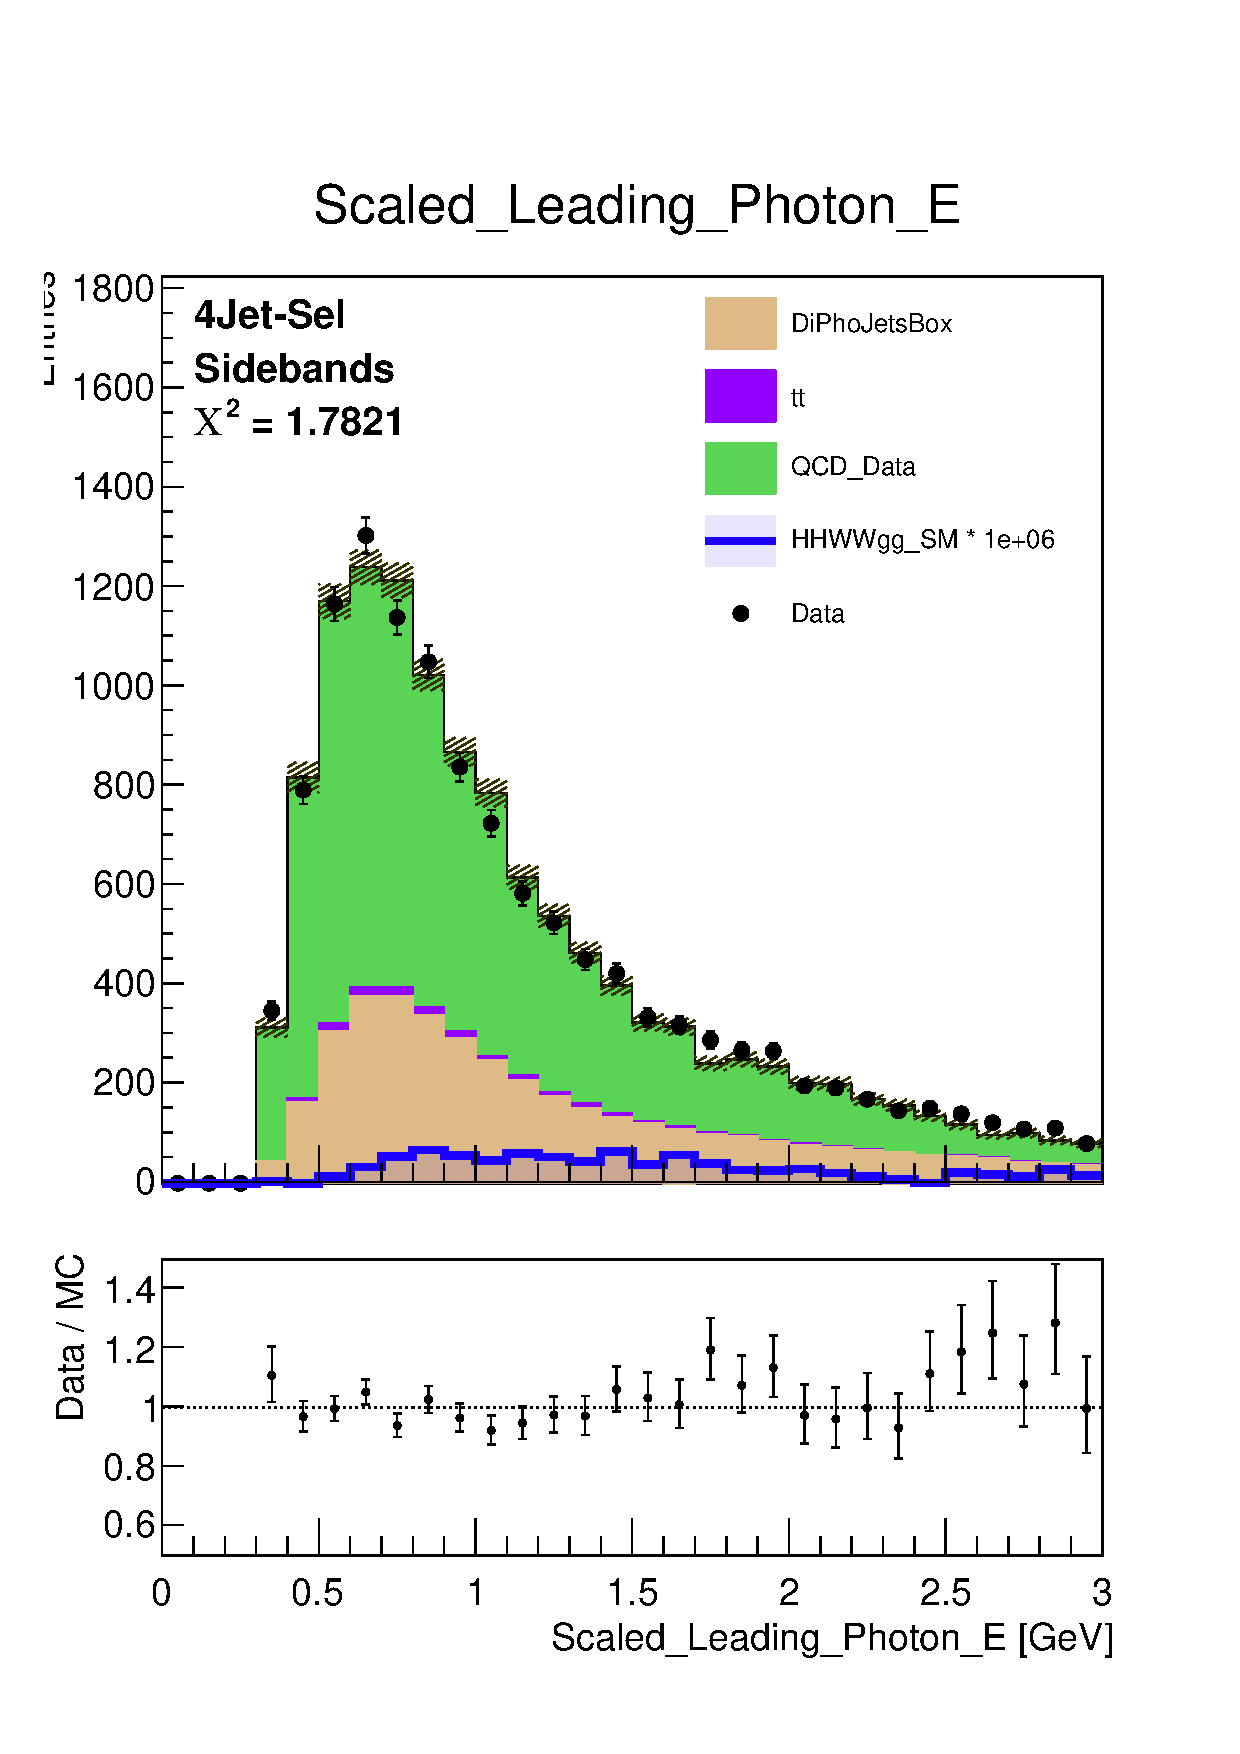
\includegraphics[width=0.45\textwidth]{Images/DataMC/DataMC_Scaled_Leading_Photon_E_SB_nonLog.pdf}%
  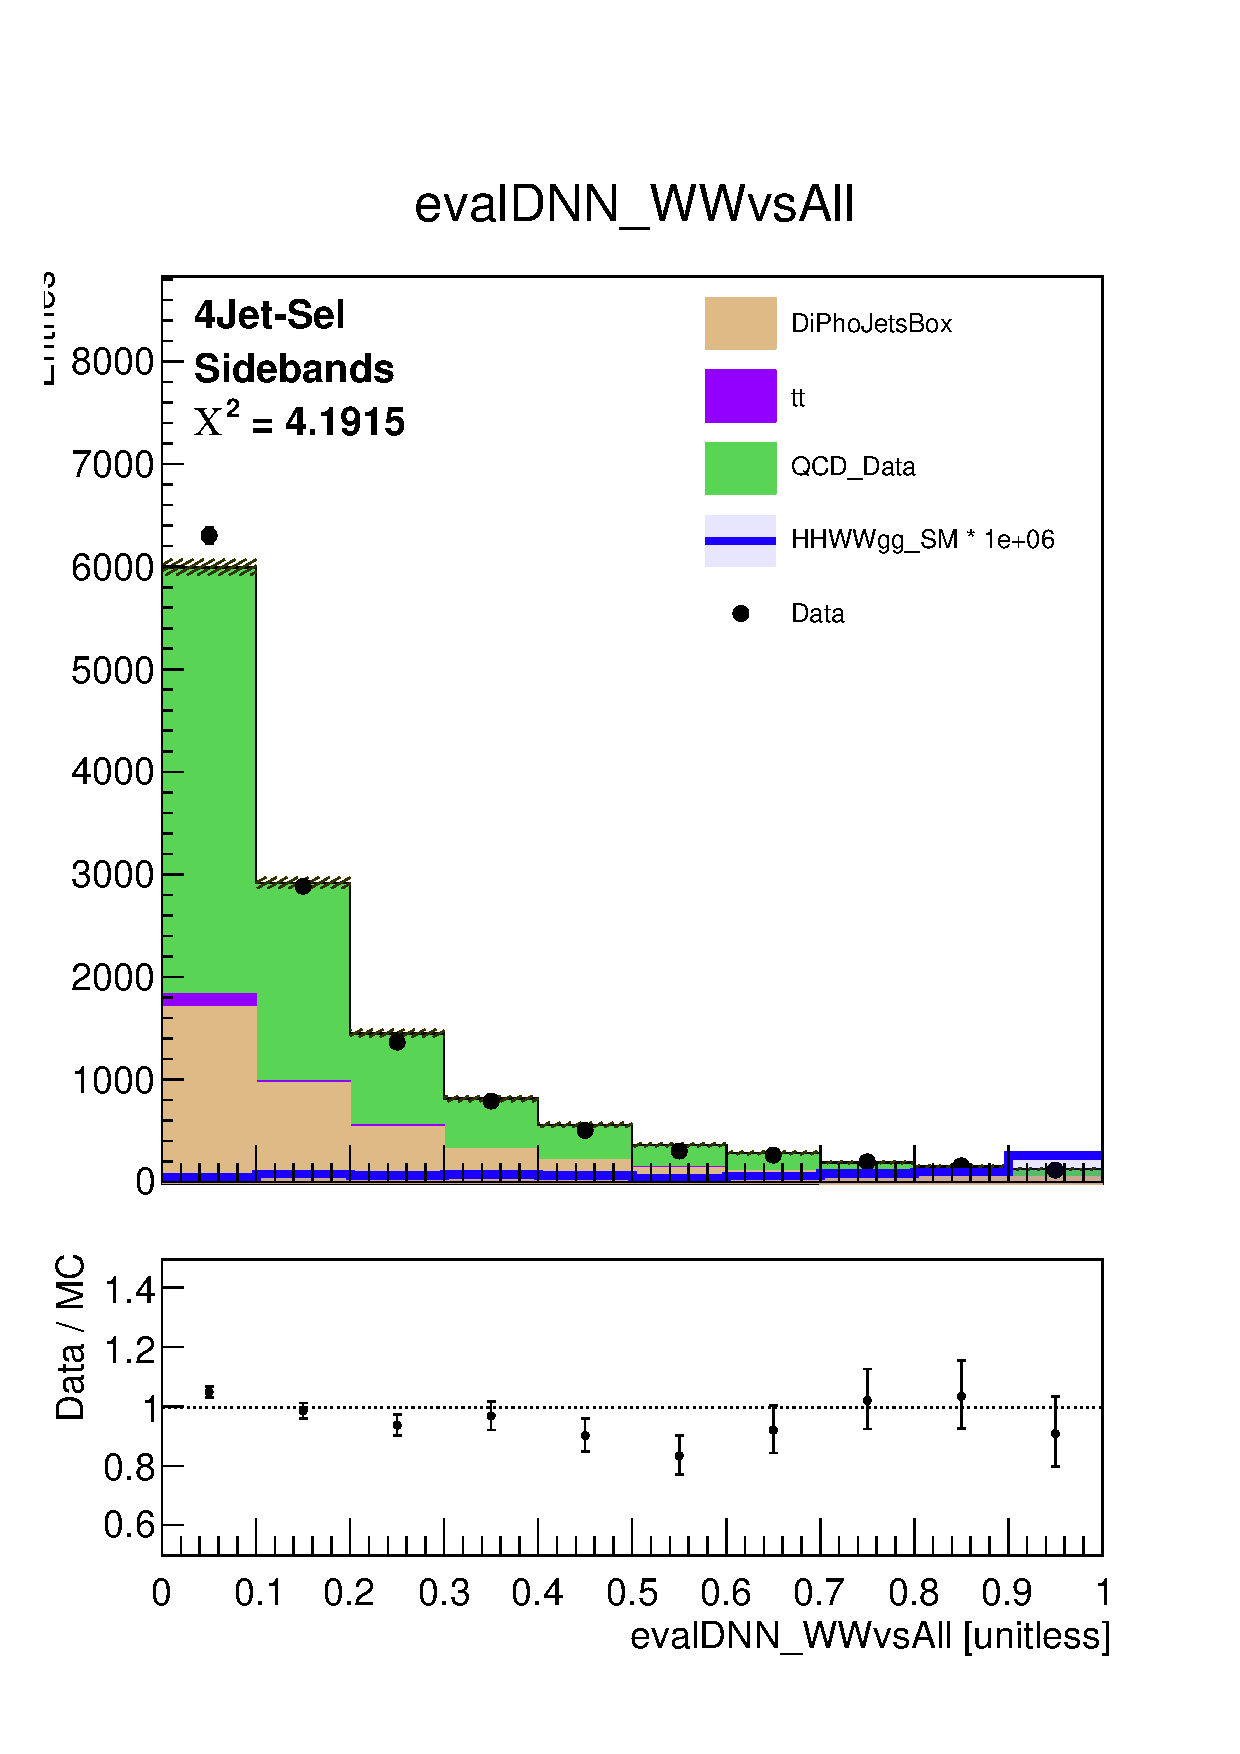
\includegraphics[width=0.45\textwidth]{Images/DataMC/DataMC_evalDNN_WWvsAll_SB_nonLog.pdf}%
  \caption{Data/MC comparison of a fully-hadronic leading DNN input feature and DNN score in the side-band region.}
\label{fig:FH_DataMC_1}
\end{figure}


% \subsection{Semi-leptonic category} \label{sec:SL_Event_Selection}

% Events fall into the SL category if they contain a diphoton candidate and exactly one lepton passing the lepton selections defined in Sec. \ref{sec:Objects}. In this final state, 
a selection is not made on b-tagging score as a preselection, in order to use this as an input feature to the DNN in order to allow it to learn how best to use this score for event discrimination.

% Events used to train the network are required to pass the Semi-Leptonic category selections described in Sec. \ref{sec:event_selection}, which require a diphoton candidate 
% and exactly one lepton passing the common lepton selections described in Sec. \ref{sec:Objects}. 

In the Semi-Leptonic category, in order to separate di-Higgs signal events from the expected single Higgs boson and continuum backgrounds, a multiclass deep neural network is 
trained to identify these three types of processes separately. This optimizes the ability to identify a region of phase space with a maximal number of HH events,
but a minimal number of single Higgs boson and continuum background events. The single Higgs boson processes are markedly different from the continuum background 
processes due to the presence of a diphoton mass peak around 125 GeV originating from the $H\rightarrow\gamma\gamma$ decay. Therefore, 
it is more logical to define these two processes separately in a DNN training rather
than defining them as part of the same class of backgrounds. 

A DNN is trained on a labelled dataset with the di-Higgs process defined as signal, and single Higgs and non-Higgs datasets defined as separate classes. The single Higgs processes
included in the training are the associated VH and ttH$+$Jet production modes of $H\rightarrow\gamma\gamma$.

The samples used for training and labeled as signal are the 12 LO benchmark samples, as well as the LO SM benchmark, where all thirteen use 2017 detector conditions.
When training on these samples, the reweighting procedure described in Sec. \ref{sec:EFT_Description}
is applied to reweight the 13 LO samples to the SM at NLO, in order to increase the statistics used to train the network to identify the SM signal. This leads to a large, statistically independent 
set of events which are reweighted to look like the SM HH signal to be used by the semi-leptonic DNN training. 

% Events used to train the network are required to pass the Semi-Leptonic category selections described in Sec. \ref{sec:event_selection}, which require a diphoton candidate 
% and exactly one lepton passing the common lepton selections described in Sec. \ref{sec:Objects}. 

The single Higgs and continuum backgrounds used in the training are those with a large yield, and with a reasonable absolute number of simulated events after the application of the Semi-Leptonic
category selections. During training, the three processes are defined as separate classes: Namely, events in the signal MC are classified as signal events, events in the single Higgs MC are classified 
as resonant background, and events in the continuum background MC are classified as continuum background. 

Due to the imbalance of the total and weighted number of events between the three datasets, 
a class weight is applied to each class in order to equalize the yields of the three classes. This ensures the network focuses on categorising all three classes with equal importance.

The features used as input to the DNN can be found in Fig. \ref{fig:DNNinputvars}.  Only basic features are used because the network is able
to learn the best way of combining features to provide optimal discrimination between signal and background.
To determine the level of optimization of the network to data, the data-MC ratio is checked for input features in the side-band regions. In order to improve data-MC agreement,
an N-dimensional kinematic reweighting is performed. A per-event weight, called a kinematic weight, is computed using the ratio between background MC and data from the $\mgg$ sideband region. 
The variables leading jet \pt, subleading set \pt, lepton pT, scaled leading photon \pt, scaled subleading photon \pt, and MET are used to calculate this per-event weight. After per events weights
are derived, a fiducial selection is made removing all events which have $|w_{MC}*w_{k}| > 10$, where $w_{MC}$ is the nominal MC weight computed from cross section, luminosity, PU weight,
scale factors and GEN weights, and $w_{k}$ represents the per event kinematic weight. This fiducial selection removes events with very large weights which heavily impact the DNN training in
a non-desirable way.

% \begin{sidewaystable}[!htbp]
% \begin{Figure}[!htbp]
\begin{figure}[!htbp]
  % \topcaption{Input features used to train semi-leptonic and fully-hadronic channel DNNs.}
  \resizebox{\textwidth}{!}{
  \begin{tabular}{| l | l | c | c |}
  \hline
  Feature & Description & Used in SL training & Used in FH trainings \\
  \hline
  Leading Photon p$_T$ / \mgg& \pt of the photon with the highest \pt out of the selected photons, scaled to diphoton mass. & \checkmark & \checkmark \\
  Leading Photon $\eta$ & Pseudorapidity of the photon with the highest \pt out of the selected photons & \checkmark & \checkmark \\
  Leading Photon $\phi$ & Direction in the transverse plane of the photon with the highest \pt out of the selected photons & \checkmark & \checkmark \\
  Leading Photon E / \mgg& Energy of the photon with the highest \pt out of the selected photons, scaled to diphoton mass. & \checkmark &   \\
  Leading Photon MVA & Photon MVA score of the photon with the highest \pt out of the selected photons & \checkmark & \checkmark \\
  Subleading Photon p$_T$  / \mgg& \pt of the photon with the second highest \pt out of the selected photons, scaled to diphoton mass. & \checkmark & \checkmark \\
  Subleading Photon $\eta$ & Pseudorapidity of the photon with the second highest \pt out of the selected photons & \checkmark & \checkmark \\
  Subleading Photon $\phi$ & Direction in the transverse plane of the photon with the second highest \pt out of the selected photons & \checkmark & \checkmark \\
  Subleading Photon E / \mgg & Energy of the photon with the second highest \pt out of the selected photons, scaled to diphoton mass. & \checkmark &   \\
  Subleading Photon MVA & Photon MVA score of the photon with the second highest \pt out of the selected photons & \checkmark & \checkmark \\
  Jet Multiplicity & Number of selected jets in the event (flavor inclusive) & \checkmark & \checkmark \\
  Lepton four-momentum & \pt, pseudorapidity, $\phi$ and energy of the selected lepton & \checkmark & \\
  MET & The missing transverse energy & \checkmark & \checkmark \\
  $M_{T}$(l, MET) & The transverse mass of the selected lepton and MET & \checkmark & \checkmark \\
  $m_{j_{0},j_{1}}$ & The invariant mass of the leading and subleading jets & \checkmark & \checkmark \\

  Leading Jet kinematics and b-score & \pt, pseudorapidity, $\phi$, energy and b-tagging score of the jet with the highest \pt out of the selected jets & \checkmark & \checkmark \\ 
  Subleading Jet kinematics and b-score & \pt, pseudorapidity, $\phi$, energy and b-tagging score of the jet with the second highest \pt out of the selected jets & \checkmark & \checkmark \\ 
  Second Subleading Jet kinematics and b-score & \pt, pseudorapidity, $\phi$, energy and b-tagging score of the jet with the third highest \pt out of the selected jets & & \checkmark \\ 
  Third Subleading Jet kinematics and b-score & \pt, pseudorapidity, $\phi$, energy and b-tagging score of the jet with the fourth highest \pt out of the selected jets & & \checkmark \\ 
  
  $\Delta \phi(HH)$ & Azimuthal separation between the two selection Higgs candidates &   & \checkmark\\
  $\Delta R(HH)$ & Separation between two Higgs in the transverse plane &   & \checkmark\\
  $min(\Delta R(g_k,j_l))$ & minimum separation between the selected jet and photon candidate &   & \checkmark\\
  $max(\Delta R(g_k,j_l))$ & maximum separation between the selected jet and photon candidate &   & \checkmark\\
  $min(\Delta R(j_k,j_l))$ & minimum separation between the jet candidates &   & \checkmark\\
  $max(\Delta R(j_k,j_l))$ & maximum separation between the jet candidates &   & \checkmark\\
  costhetastar & The angle between the parton collision axis $z$ and the $pp\rightarrow H_1H_{2}$ decay axis $z'$, both defined in the $H_1H_{2}$ system rest frame &   & \checkmark \\
  costheta1 & Angle between the direction of the W-boson ($W_1$) from the $H_1\rightarrow W_1 W_2$ and the direction opposite the $H_1H_2$ in the $H_1$ rest frame. &   & \checkmark\\
  costheta2 & Angle between the direction of the W-boson ($W_2$) from the $H_2\rightarrow \gamma \gamma$ and the direction opposite the $H_1H_2$ in the $H_2$ rest frame. &   & \checkmark\\
  Phi & Angle between the decay planes of the two Z-system in the $H_1H_2$ rest frame &   & \checkmark\\
  Phi1 & Angle between the $zz'$ plane and the plane of the $H_{1}\rightarrow \gamma \gamma$ decay in the $H_{1}H_{2}$ rest frame &   & \checkmark \\
  W1 pT & pT of vector sum of two leading jets &   & \checkmark\\
  W1 $\eta$ &  rapidity of vector sum of two leading jets &   & \checkmark\\
  W1 mass &  Invariant mass of vector sum of two leading jets &   & \checkmark\\
  
  W2 pT & pT of vector sum of 3rd and 4th leading jets &   & \checkmark\\
  W2 $\eta$ & rapidity of vector sum of 3rd and 4th leading jets &   & \checkmark\\
  W2 mass & Invariant mass of vector sum of 3rd and 4th leading jets &   & \checkmark\\
  
  WW pT & pT of vector sum of first four leading jets &   & \checkmark\\
  WW $\eta$ & rapidity of vector sum of first four leading jets &   & \checkmark\\
  WW mass & Invariant mass of vector sum of first four leading jets &   & \checkmark\\
  
  \hline
  \end{tabular}
  }
  % \label{tab:DNNinputvars}
\caption{Input features used to train semi-leptonic and fully-hadronic channel DNNs. \label{fig:DNNinputvars}}
\end{figure}
% \end{sidewaystable}

Because the three classes are globally scaled to have matching yields in the training, a single Data/MC weight is extracted and applied in order to compare the data and MC input feature shapes.
The weight is obtained and a shape comparison is performed
in the following way: First, MC is scaled to the ratio of data / MC integrals
in the full mass region, 100 $<$ $\mgg$ $<$ 180 GeV. Then, events with an output DNN discriminant score less than 0.1 are removed before the ratio of data / MC
integrals is computed, to only show the data / MC agreement of events which are used in the Semi-Leptonic categorization and fitting. In this analysis, events with a DNN score less than 0.1 
are removed, and therefore are not used in categorization, nor in any analytic fitting. This is done because this region contains a large portion of background, and a very low portion of signal, and therefore has a negligible impact on the sensitivity of the analysis. Additionally,
this region is not used as a control region to reduce the uncertainty of MC in the signal region.

The MultiClass DNN outputs three DNN scores, each corresponding to the likelihood that an event falls into each of the three classes, which sum to one, and are back-propogated
to optimize the DNN weights. This also means that if an event has a high HH class DNN score, the sum of the H and continuum background DNN scores must be small. As there is no need to separate 
the single Higgs and continuum background processes from each other, only the output HH class DNN score is used in the analysis for categorization.

Several architectures were investigated in an attempt to give the model enough flexibility to model decision boundaries in high-dimensionality
phase-space, while ensuring the model is trainable with the size of our dataset. Once the network's architecture was established, a hyper-parameter scan was performed on the number of epochs, 
learning rate and batch size. The performance of the network was found to be relatively robust to further fine-tuning of hyper-parameters.

The leading importance input features of the network, according to their Shapley values, are the leading and subleading photon $\pt$ taken as a ratio to the invariant diphoton mass, 
the energy of the lepton, and the $\pt$ of the subleading jet. 

The output DNN score comparison between the data and MC for a leading importance variable and the HH DNN score is shown in Figure \ref{fig:SLDNNFeaturecontrolplots-1}. Four categories are defined, with the corresponding DNN score boundaries: 
[0.1, 0.63, 0.84, 0.89, 1.0].

% Note that as the DNN output score is 
% used to categorize events but is not used as a shape in the extraction of any results, any disagreements between data and simulation could lead to a sub-optimal network, but would not lead to any bias in the 
% final results. 

\begin{figure}[!htbp]
  \setcounter{subfigure}{0}
  \centering
  \subfloat[Scaled Leading Photon pt]{\includegraphics[width=0.45\textwidth]{Images/DNN/DataMC/DataMC_Scaled_Leading_Photon_pt_FullRegion_log.pdf}}
  \qquad
  \subfloat[DNN output score]{\includegraphics[width=0.45\textwidth]{Images/DNN/DataMC/DataMC_evalDNN_HH_FullRegion_log.pdf}}
  \caption{Data/MC ratio of semi-leptonic channel leading input feature, and DNN score in diphoton mass region 100 $<$ $\mgg$ $<$ 180 GeV.}
  \label{fig:SLDNNFeaturecontrolplots-1}
\end{figure}

In addition, a separate parametric binary DNN is trained in order to categorize signatures from the twenty EFT benchmark hypotheses defined in Tab. \ref{tab:eft_bench}. A parametric DNN is a
neural network which, in this case, includes the EFT benchmark number as an input variable. This allows one to train a DNN which can effectively produce 20 output scores, based on different 
input values of the node hypothesis, rather than having to train 
20 separate DNN's. This method is particularly useful for training a DNN to categorize events for the 20 EFT benchmark nodes in this analysis. A single DNN training is performed, using 
4 NLO samples reweighted to the 20 EFT benchmarks at NLO as signal, with the same single Higgs and continuum background MC samples used as backgrounds in the training as were used for the DNN 
trained to identify the SM HH signal. Category boundaries are optimized for each node hypothesis scenario, based on expected sensitivity. 


% \subsection{Fully-leptonic category}

% For events to fall into the FL analysis category, they must contain exactly two oppositely charged leptons ($e^{+}e^{-}$, $\mu^{+}\mu^{-}$, $e^{\pm}\mu^{\mp}$).
% The leading \pt lepton is required to have \pt $>$ 20$\GeV$, the subleading lepton is required to have \pt $> 10\GeV$, and a distance parameter between the two leading \pt leptons $>$ 0.4 is required.
% Events are rejected from this category if the event contains a third lepton with \pt $> 10\GeV$ in order to avoid saving events with three high energy leptons, as only two 
% are expected from this process. In order to identify events with missing transverse momentum due to the two neutrinos from the 
% leptonically decaying W-bosons, events are required to have $p_T^{miss} > 20 \GeV$. Furthermore, the diphoton candidate in this final state is required to have \pt $> 91 \GeV$, 
% an invariant mass between each electron candidate and photon candidate which is at least 5 GeV different from the invariant Z boson mass to avoid saving Z$\rightarrow\ell\ell$ events. The invariant mass 
% from the two leading leptons is required to be $<$ 80 GeV or $>$ 100 GeV in order to suppress VH(H$\rightarrow\gamma\gamma$) events, as shown in Fig.\ref{fig:FL_dilepmass}. In addition, events containing at least one jet 
% with a b-tagging score greater than a medium working point are removed. The reason a b-veto is applied in this final state and not for the SL and FH final states is because this final state applies 
% a cut-based selection, and therefore we choose to apply a b-veto as part of the final selections. 

% \begin{figure}[!htbp]
%   \begin{center}
% 	\includegraphics[width=0.9\textwidth]{Images/Selections/FL_CutBased/DiLeptonMass.pdf}
%     \caption{
%       $m_{ll}$ distribution comparison between signal and VH events, where the signal and VH distributions have been normalized to 1, and the two dashed lines show the final cuts on the di-Lepton mass: $m_{ll}$ $< 80\GeV$ or $m_{ll}$ $> 100\GeV$ .
%     }
%     \label{fig:FL_dilepmass}
%   \end{center}
% \end{figure}


\section{Signal and background modelling} \label{sec:AnalyticFitting}

In order to model the di-Higgs signal process, and single higgs resonant background processes in the signal region, 115 $< \mgg < $ 135 GeV, simulated events 
in each analysis category are combined to construct $\mgg$ shapes. Because the continuum background in the signal region is expected to follow a falling 
shape continuous with the data sidebands, data events in the data sidebands are fit to a falling analytic function in order to model the continuum background. 

\subsection{Di-Higgs signal}
\label{sec:SignalFitting}

Signal shapes for the invariant mass distribution of the diphoton candidate are derived for all analysis categories using simulated events. 

Signal models are formed by an analytic fit of a sum of 1-5 Gaussians to a binned $\mgg$ distribution, where the chosen number of Gaussians used in the fit is 
determined by an F-test. This is done separately for each year (2016, 2017, 2018) and each analysis category.
The fit for the second highest DNN score region FH category is shown 
in Fig.  \ref{fig:FHSignalModel} . 



\begin{figure}[!htbp]
  \centering
  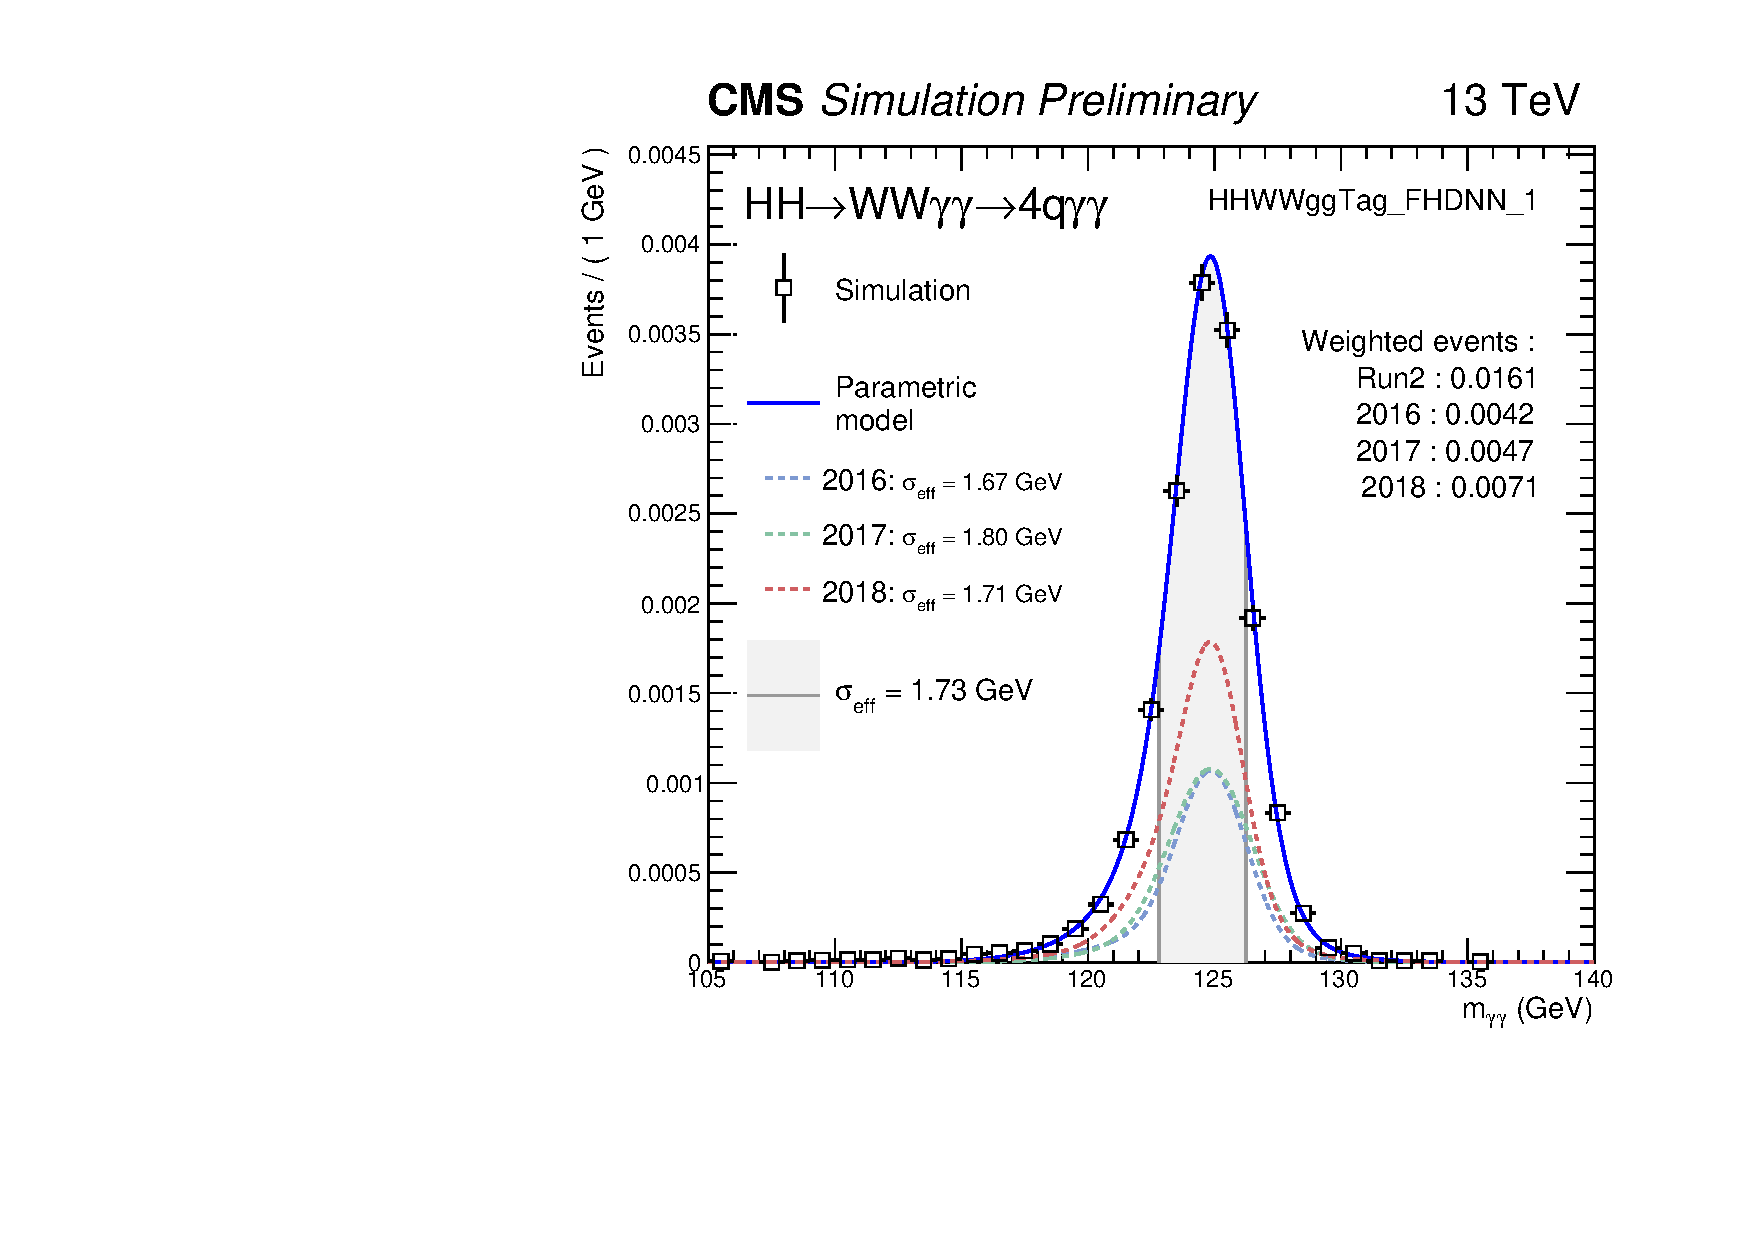
\includegraphics[width=0.75\textwidth]{Images/AnalyticFitting/Signal/smodel_HHWWggTag_FHDNN_1.pdf}
  \caption{FH signal model in the second most sensitive category}
\label{fig:FHSignalModel}
\end{figure}

\subsection{Single Higgs background}

There are expected resonant background processes present in the signal region, $115 < \mgg < 135$ GeV, due to $H\rightarrow\gamma\gamma$ processes, which cannot be modeled with a data-driven
method using data sideband events. These backgrounds are modeled with MC in the same fashion as the $HH\rightarrow WW\gamma\gamma$ signals as described in Sec. \ref{sec:SignalFitting}. The single higgs
processes considered as resonant backgrounds are the gluon-gluon fusion, vector boson fusion, associated production with a vector boson, and associated production with a top quark pair (ttH), where the Higgs boson decays 
into two photons. A separate fit is made for each analysis category and production mode. For cases in which there is a very small number of MC statistics, the diphoton shape from 
the di-Higgs signal model in the same analysis category is taken and scaled to the single higgs yield in this category, and used to model the single higgs shape in this category. 

\subsection{Continuum background}
\label{sec:AnalyticFitting_Background}

A data-driven background model is produced for each category using the data sidebands in the regions $100 < \mgg < 115$ GeV and $135 < \mgg < 180$ GeV.
The aim of this is to model the continuum background.
After the event selections and categorizations described in Sec. \ref{sec:event_selection} are applied, analytic functions are fit to the resulting $\mgg$ distributions in the data sidebands for each category.
These are later combined with their corresponding signal models in order to extract final results.
As with the signal fitting, an F-Test is performed first in order to obtain initial best-fit estimates for backgrounds functions to the data-sidebands, and to determine which functions will be considered.
Bernstein, laurent, exponential, and powerlaw function families are considered as
candidates to fit the data, and F-Tests are performed for each of these. The three data taking years are merged together before the F-test and function fitting is performed. 
After determining which functions pass the F-Test, a best fit function is chosen with the envelope method by treating the choice of function as a discrete nuisance parameter.
An uncertainty is then assigned to the chosen fit function based on a combination of the likelihoods of all attempted fit functions. This method is described in
Ref. \cite{Dauncey_2015}.

After obtaining signal models, continuum background models and Single-Higgs models for each final state, a signal plus background fit is performed.
The combination of all categories' signal plus background fits in the range 100 $<$ $\mgg$ $<$ 180 GeV, where each category is weighted by S over S$+$B, is shown in Figure \ref{fig:Run2SplusB}.

\begin{figure}[!htbp]
  \centering
  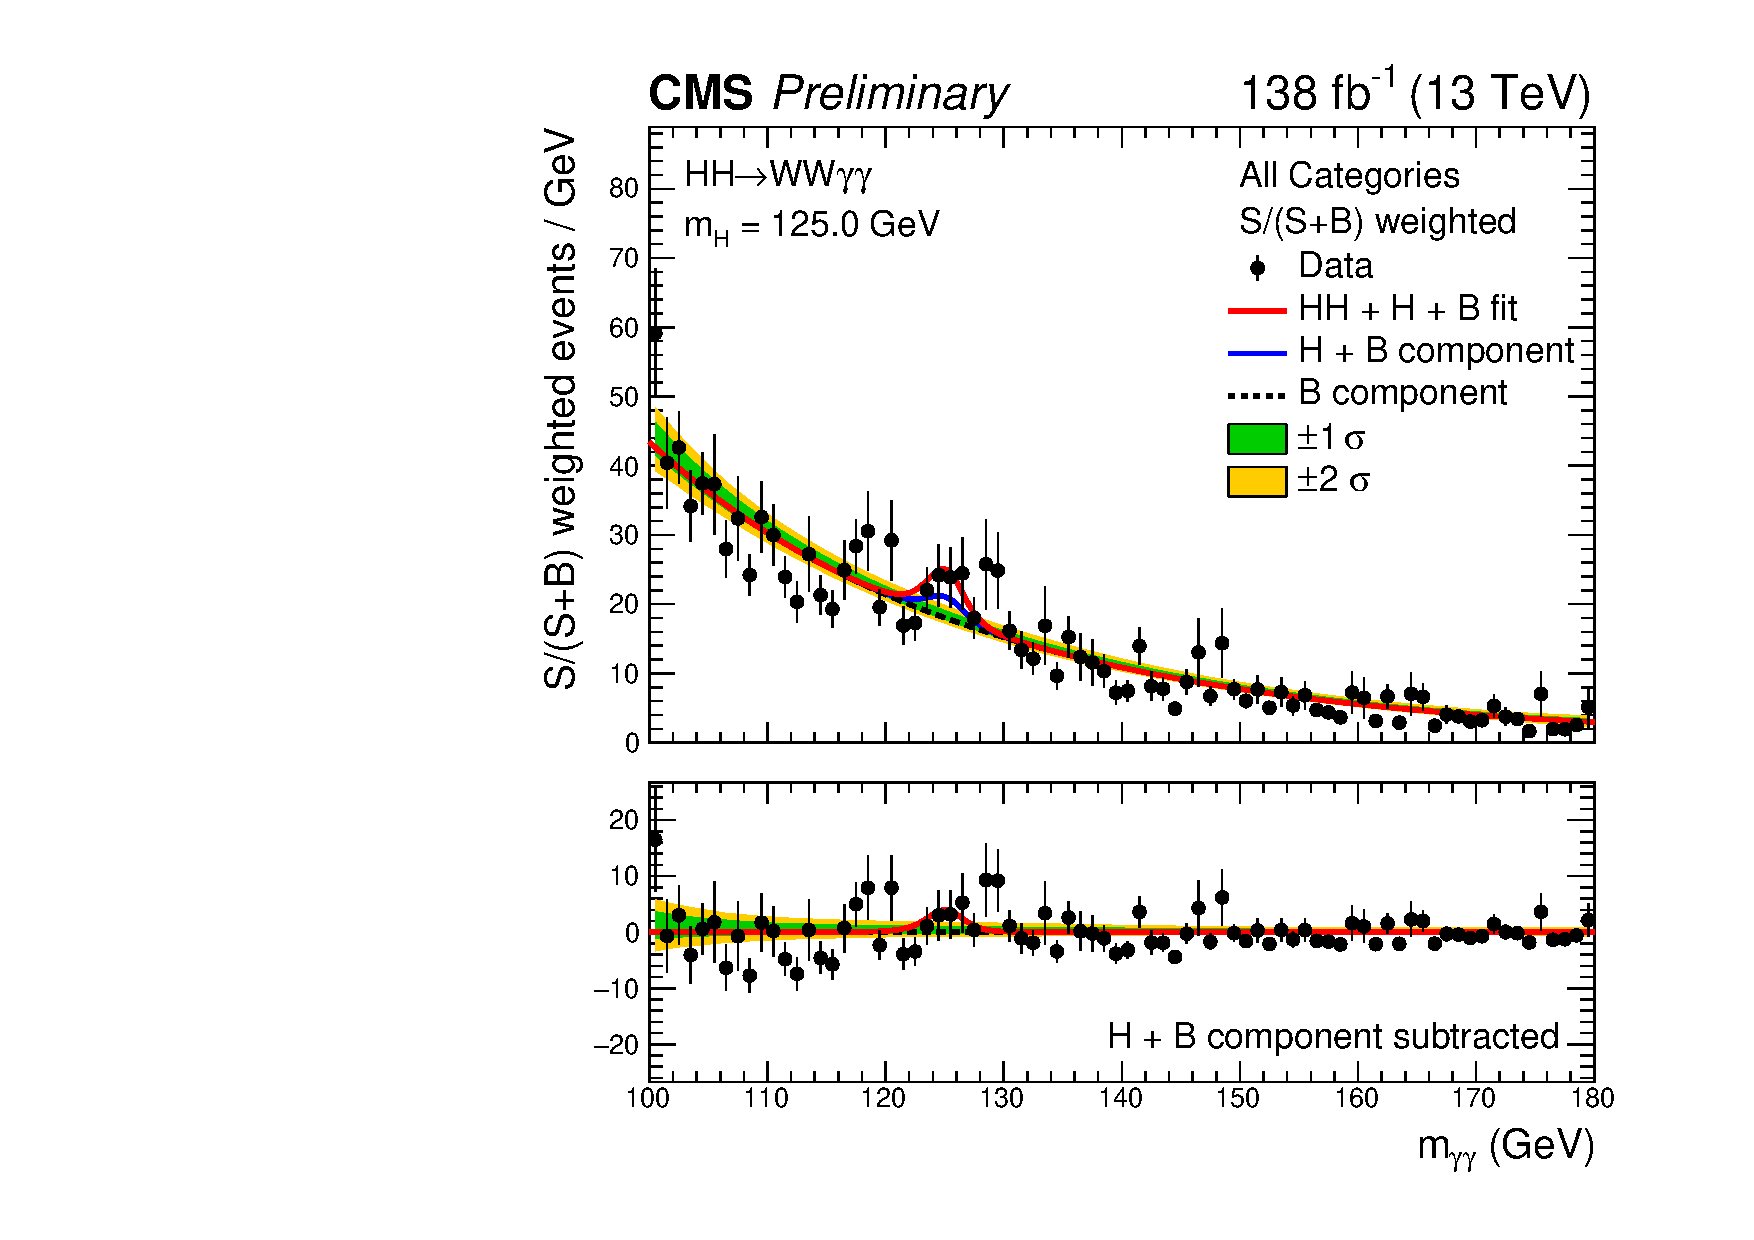
\includegraphics[width=0.9\textwidth]{Images/Results/All_combined_SplusB.pdf}
 \caption{The observed diphoton mass distribution including the signal plus background fit (red), the Single-Higgs + continuum background fit (blue) and the continuum background (black dashed line), 
 with bands covering the $\pm 1\sigma$ and $\pm 2\sigma$ uncertainties in the fitted background where all analysis categories are combined and weighted by S over S$+$B.}
  \label{fig:Run2SplusB}
\end{figure}

\section{Systematic uncertainties} \label{section:Systematics}
This analysis takes into account systematic uncertainties from theoretical and experimental sources. The uncertainties on the signal and on the single Higgs backgrounds are modeled as scale or shape uncertainties. The scale uncertainties affect the yield of the processes and are treated as log-normal uncertainties, while the shape uncertainties are modeled as variations of the \mgg shape of the processes, i.e. the peak position or the width. The systematic uncertainty associated with the data-driven estimate of the continuum background is accounted for via the discrete profiling method. Given the small number of expected signal events compared to the backgrounds, the effect of the systematics uncertainties on the final results is expected to be small compared to the statistical ones. In case a systematic uncertainty affects processes in different channels, it is considered fully correlated across those channels. The following sources of systematic uncertainties are considered:

\begin{enumerate}

  \item \textbf{Theoretical uncertainties on the HH cross section}: The combined uncertainty on the QCD scale and on the top mass is taken into account, considering also its dependence from the value of $\kappa_{\lambda}$. For the SM signal this uncertainty amounts to $-23/+6\% $. The combined uncertainty on the PDF modeling and on the strong coupling constant is also considered with a value of $3\% $ \cite{Grazzini:2018bsd}. 

  \item \textbf{Theoretical uncertainties on the single Higgs cross sections}: Process-dependent uncertainties related to the QCD scale, the PDF modeling, and the strong coupling constant are taken into account for the ggH, ttH, VBF H, and VH processes.

  \item \textbf{Theoretical uncertainties on the Higgs boson branching ratios}: Such uncertainties are considered for both the single and the double Higgs processes. The considered uncertainties on the $H\rightarrow\gamma\gamma$, $H\rightarrow VV$, and $H\rightarrow bb$ branching ratios are approximately $2\% $, $1.5\% $, and $1.2\% $, respectively. 

  \item \textbf{Integrated luminosity}: A scale uncertainty is defined according to the luminosity measurements performed by the CMS experiment ~\cite{CMS-LUM-17-003,CMS-PAS-LUM-17-004,CMS-PAS-LUM-18-002}.

  \item \textbf{Trigger}: The trigger efficiency is measured from data with a tag and probe procedure using $Z \rightarrow ee$ events. The related uncertainty is uncorrelated between the three data taking years. An additional considered source of uncertainty is related to inefficiencies of the ECAL L1 trigger at $|\eta|>2$ experienced during 2016 and 2017. This is modeled as a purely rate-changing uncertainty.

%  \item \textbf{Pile-up reweigthing}: The distribution of the simultaneous number of interactions in the Monte Carlo simulation is corrected to match the one observed in the data through an event reweight procedure. The uncertainty on the number of pile-up events is estimated by varying the proton-proton inelastic cross section, 69.2 mb, within $\pm$ 4.6\%. This is modeled as a scale uncertainty uncorrelated between the three data taking years. 

  \item \textbf{Electron and muon reconstruction, identification and isolation efficiency}: These efficiencies are evaluated in data and simulation with tag-and-probe techniques using Drell-Yan events \cite{Khachatryan:2015hwa, Sirunyan:2018fpa}. Scale factors are derived and applied to the simulated events to improve the agreement of the efficiencies between simulation and data. The related uncertainty is purely rate-changing and uncorrelated between the three data taking years.

  \item \textbf{Photon identification}: The efficiency of the pre-selection on the photon identification MVA score is estimated in data and simulation with a tag-and-probe technique using Drell-Yan events. Scale factors are applied to correct for the difference between the data and the simulation. The related uncertainty is purely rate-changing  and uncorrelated between the three data taking years.        

%  \item \textbf{Electron energy scale and resolution}: Corrections for the energy scale observed in the data are applied to match the simulated one, and for the energy resolution observed in the simulation to match the one observed in the data. The systematic uncertainty on the electron energy scale and resolution is taken considering the POG provided resolution error and the uncertainty on the electron $p_T$. This uncertainty is uncorrelated between the three data taking years.

  \item \textbf{Photon shower shape}: Corrections for the imperfect modeling of the photon shower shape (and isolation) variables in simulation are applied to improve the agreement with the data. The impact of this uncertainty is estimated from the difference of the photon energy scale before and after the correction. This is modeled as a shape uncertainty which is correlated between the three years of the data taking.

  \item \textbf{Photon energy scale and resolution}: Corrections for the difference of the photon energy scale and resolution between data and simulation are derived using $Z \rightarrow ee$ events, with electron-photon differences accounted for as a systematic uncertainty. This uncertainty is uncorrelated between the three years of the data taking.

% Not sure if we apply this. Check: https://github.com/atishelmanch/flashgg/blob/HHWWgg_dev/Taggers/interface/HHWWggTagProducer.h 
%   \item \textbf{Di-photons vertex identification efficiency}: Scale factors are computed to account for the difference between data and simulation in number of events for which the correct vertex has been selected. 

  %https://twiki.cern.ch/twiki/bin/view/CMS/JECUncertaintySources#Recommendation_for_analysis
  \item \textbf{Jet energy scale and resolution}: Corrections for the differences in the measured jet energies between data and simulation are applied \cite{Khachatryan:2016kdb}. The impact of the corresponding uncertainties on the signal yield is evaluated by varying the corrected jets four-momentum within their respective per-jet uncertainties and propagating the effect to the final result. Several sources of uncertainty are considered, each with a specific level of correlation among the three years of data taking. 

  \item \textbf{B-tagging}: The difference in the b-tagging score distribution between data and simulation is corrected for with a reweight of the simulated events dependent on the jet $p_T$, $|\eta|$, and flavor \cite{Sirunyan:2017ezt}. The corresponding uncertainty is purely rate-changing and uncorrelated between the three years of data taking.

%   \item \textbf{b-tagging scale factors}: Applied to each jet as a function of jet $p_T$ and $|\eta|$ in order to account for the efficiency difference in b-tagging and misidentification 
%         between data and Monte Carlo simulation \cite{Sirunyan:2017ezt}. The systematic effect is estimated by shifting the scale factor up and down by $\sigma$. 
%         The \textbf{1a} method \cite{BtaginMethods} is used to predict the correct event yield in data by changing the weight of the selected Monte Carlo events. This uncertainty is uncorrelated between the three 
%         data taking years.



  
\end{enumerate}

The systematic uncertainties due to finite statistics of Monte Carlo samples for the HH signal are neglected.

\section{Results} \label{sec:results}

The SM hypothesis tested in this analysis is the existence of the SM non-resonant di-Higgs process, probed via the WW$\gamma\gamma$ phase space. Additionally, BSM hypotheses are tested in the context of the 
EFT framework described in Section \ref{sec:EFT_Description}, including a di-Higgs process whose production cross section is altered due to the modification 
of the di-Higgs self-coupling, coupling of two Higgs bosons to two top quarks, and a group of 20 EFT benchmark nodes corresponding to modifications 
of $\kappa_{\lambda}$, $\kappa_{t}$, $c_{2}$, $c_{g}$, $c_{2g}$ defined in Tab. \ref{tab:eft_bench}. 

Expected (observed) results are obtained by performing a simultaneous likelihood fit of the signal and 
background templates to Asimov (observed) data, in categories defined by selections a combination 
of two binary DNN's. For the $\kappa_{\lambda}$ scan, the same categorization methods are used as for the 
SM case, but applied to three HH simulated samples corresponding to $\kappa_{\lambda}$ = [1, 2.45, 5], where a weighted linear combination and shape interpolation of the three is made in order to estimate 
the expected yield and shape for $\kappa_{\lambda}$ hypotheses between -30 and 30. The effects of anomalous $\kappa_{\lambda}$ values on the Higgs boson branching ratios and on the single Higgs cross sections are taken into account using the modeling provided in Ref.~\cite{Degrassi:2016wml} and \cite{Maltoni:2017ims}.

For the $c_{2}$ scan, a similar approach is taken but with the use of 6 EFT signal models obtained via a reweighting of 4 NLO samples. 

The 20 EFT benchmark node results are extracted in categories defined based on a reweighting of SM MC events.  

As it is not possible to observe a signal given the sensitivity of the analysis on the available dataset, a modified frequentist method $CL_s$ \cite{CLS1, CLS2} is used to 
calculate the 95\% confidence-level ($CL_{s}$) exclusion limits with the asymptotic approximation \cite{Cowan:2010js}. This method is applied in order to determine the upper limit 
on the production cross section of each signal hypothesis. Each upper limit is extracted by positively scaling the corresponding 
HH signal model until it is incompatibile with the background-only hypothesis (expected), or data (observed), at a 95\% $CL_{s}$.   

Combining all categories of FH WW$\gamma\gamma$ (+ZZ$\gamma\gamma$+bb$\gamma \gamma$  channels leads to the combined Run 2 results shown in Table \ref{tab:Run2Results}.

\begin{table}[h!]
  \begin{center}
    \begin{tabular}{|c|ccccc|}
      \hline
         Observed limit & $-2\sigma$ & $-1\sigma$ & Expected Limit & $+1\sigma$ & $+2\sigma$ \\ \hline
        %   278.2   &   81.4 & 119.3 & 189.4 & 326.8 & 546.7  \\ \hline
          312.6  &   70.4 & 97.6 & 143.0 & 228.5 & 352.6   \\ \hline
        %   71.3  &   29.5 & 41.9 & 64.0 & 106.3 & 170.4 \\ \hline
        %   96.8  &   24.8 & 35.0 & 52.5 & 85.6 & 134.8  \\ \hline
          \end{tabular}
  \end{center}
  \caption{Full Run2 Combination results
  on $\frac{\sigma(HH)}{\sigma_{SM}(HH)}$, assuming an NLO standard model cross section of about 31.05 fb}
  \label{tab:Run2Results}
\end{table}  

% \begin{table}[h!]
%   \begin{center}
%     \begin{tabular}{c|c|ccccc}
%       \hline
%         & Observed limit & $-2\sigma$ & $-1\sigma$ & Expected Limit & $+1\sigma$ & $+2\sigma$ \\ \hline
%           Fully-Leptonic &  278.2   &   81.4 & 119.3 & 189.4 & 326.8 & 546.7  \\ \hline
%           Fully-Hadronic &  312.6  &   70.4 & 97.6 & 143.0 & 228.5 & 352.6   \\ \hline
%           Semi-Leptonic  &  71.3  &   29.5 & 41.9 & 64.0 & 106.3 & 170.4 \\ \hline
%           Combination    &  96.8  &   24.8 & 35.0 & 52.5 & 85.6 & 134.8  \\ \hline
%           \end{tabular}
%   \end{center}
%   \caption{Full Run2 Combination results, including SL, FL and FH categories,
%   on $\frac{\sigma(HH)}{\sigma_{SM}(HH)}$, assuming an NLO standard model cross section of about 31.05 fb}
%   \label{tab:Run2Results}
% \end{table}  

A combined median value of 96.8 (52.5 expected) times the NLO approximation of the standard model gluon gluon HH cross section is obtained, considering a standard model cross section of 31.05 fb. 

The combined $\kappa_{\lambda}$ scan is shown in Figure \ref{fig:Combined_kl}, with each category and the combined median limit values shown
in Figure \ref{fig:Channel_kl}. Note that the theory prediction line, drawn in red, represents the predicted HH cross section value for a certain value of $\kappa_{\lambda}$.

As shown in Figure \ref{fig:Combined_kl}, an observed (expected) constraint on the Higgs self-coupling of -25.80 (-14.43) to 24.10 (18.33) times its standard model value 
is obtained at a 95\% CL. 

The combined $c_{2}$ scan is shown in Figure \ref{fig:Combined_c2}, with each category and the combined median limit values shown
in Figure \ref{fig:Channel_c2}. Note that the theory prediction line, drawn in red, represents the predicted HH cross section value for a certain value of $c_{2}$.

As shown in Figure \ref{fig:Combined_c2}, an observed (expected) constraint on the coupling constant magnitude of two top quarks to two Higgs bosons of
-2.42 (-1.75) to 2.88 (2.21) is extracted at a 95\% CL.

Finally, the observed (expected) upper limits on the production cross section of the 20 EFT benchmark scenarios defined in Tab. \ref{tab:eft_bench} are shown in 
Fig. \ref{fig:20_EFT_benchmark_results_all}, and range from 1.7 - 6.2 (1.0 - 3.9) pb. 

\begin{figure}[!htbp]
  \centering
  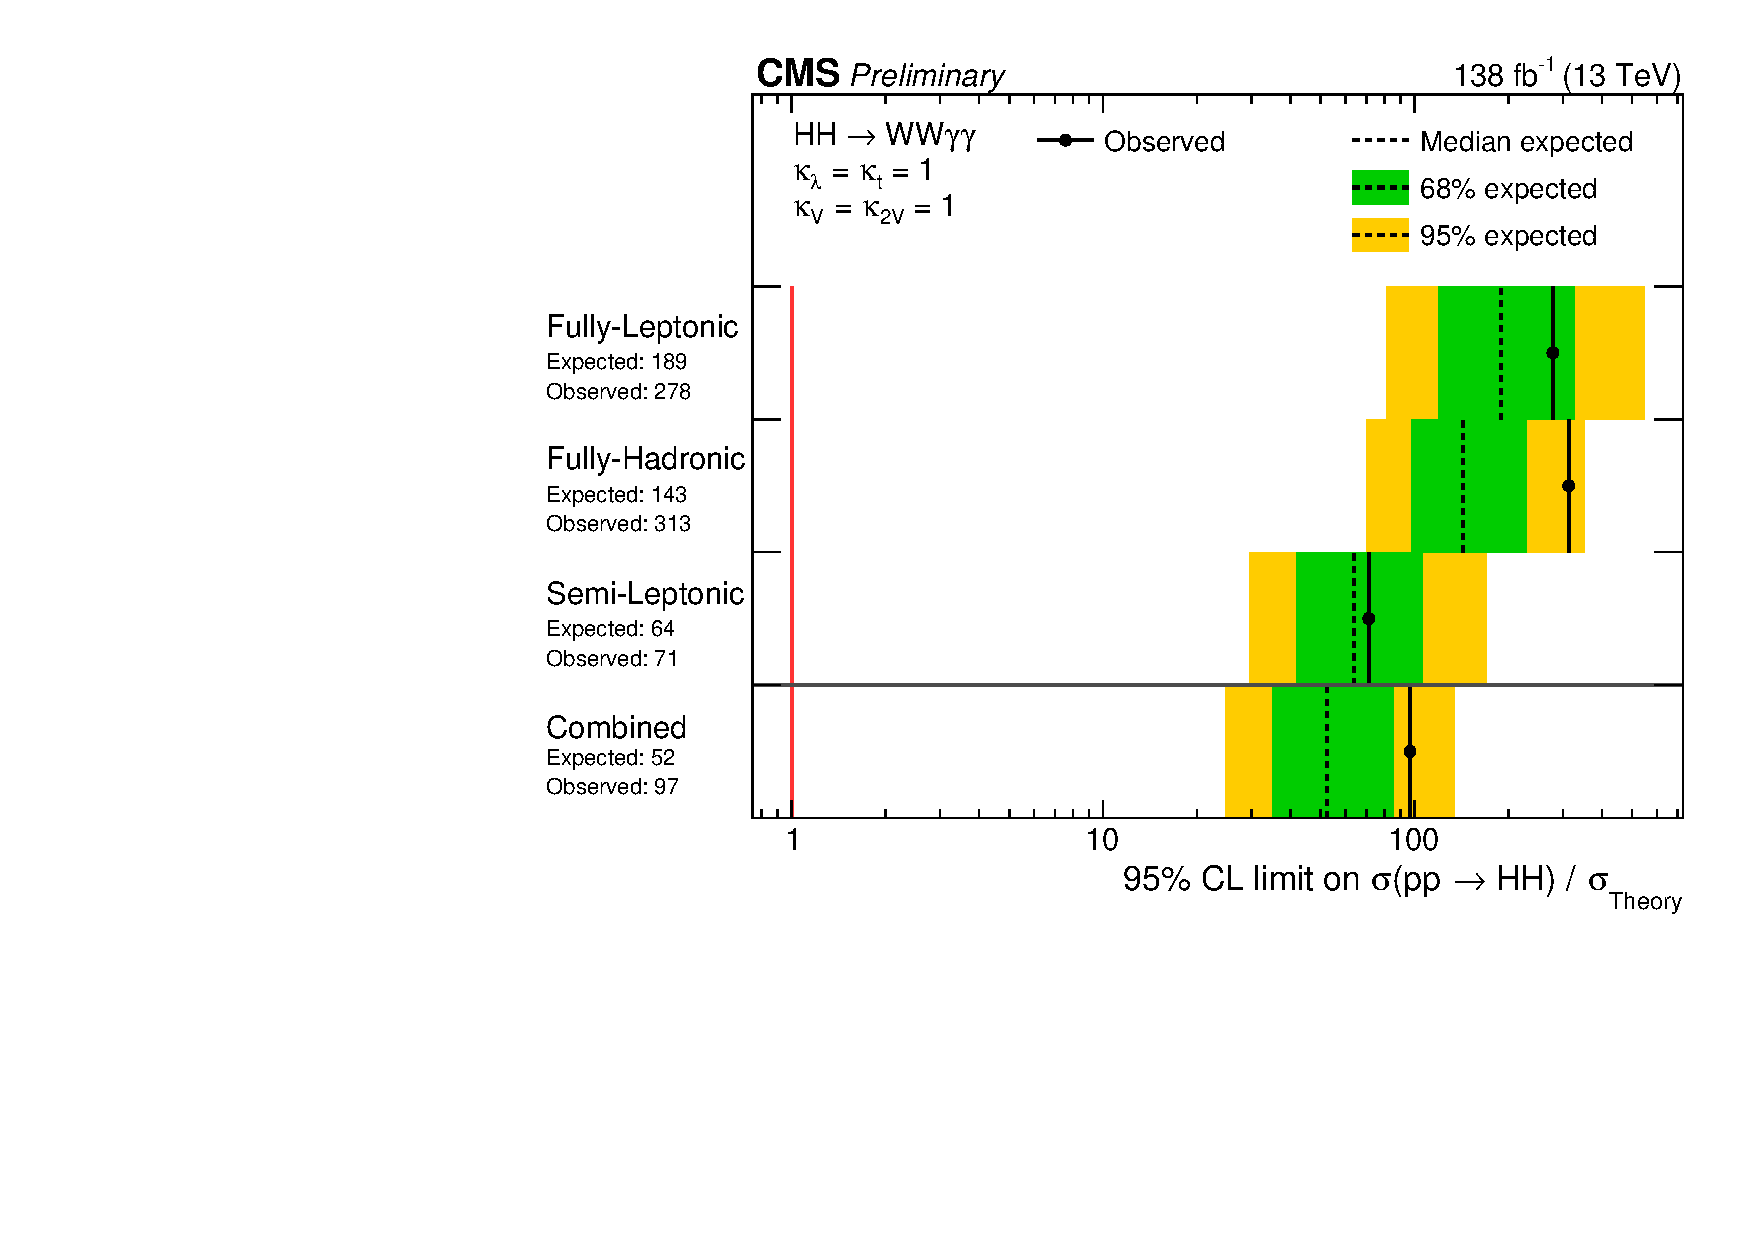
\includegraphics[width=0.7\textwidth]{Images/Results/All_limits.pdf}
  \caption{Run 2 95\% $CL_{s}$ limits on HH gluon gluon fusion production with respect to $\sigma_{SM}^{NLO} \approx $ 31.05fb}
  \label{fig:Run2SMNLOCombined}
\end{figure}

\begin{figure}[!htbp]
  \setcounter{subfigure}{0}
  \centering
  \subfloat[Per channel]{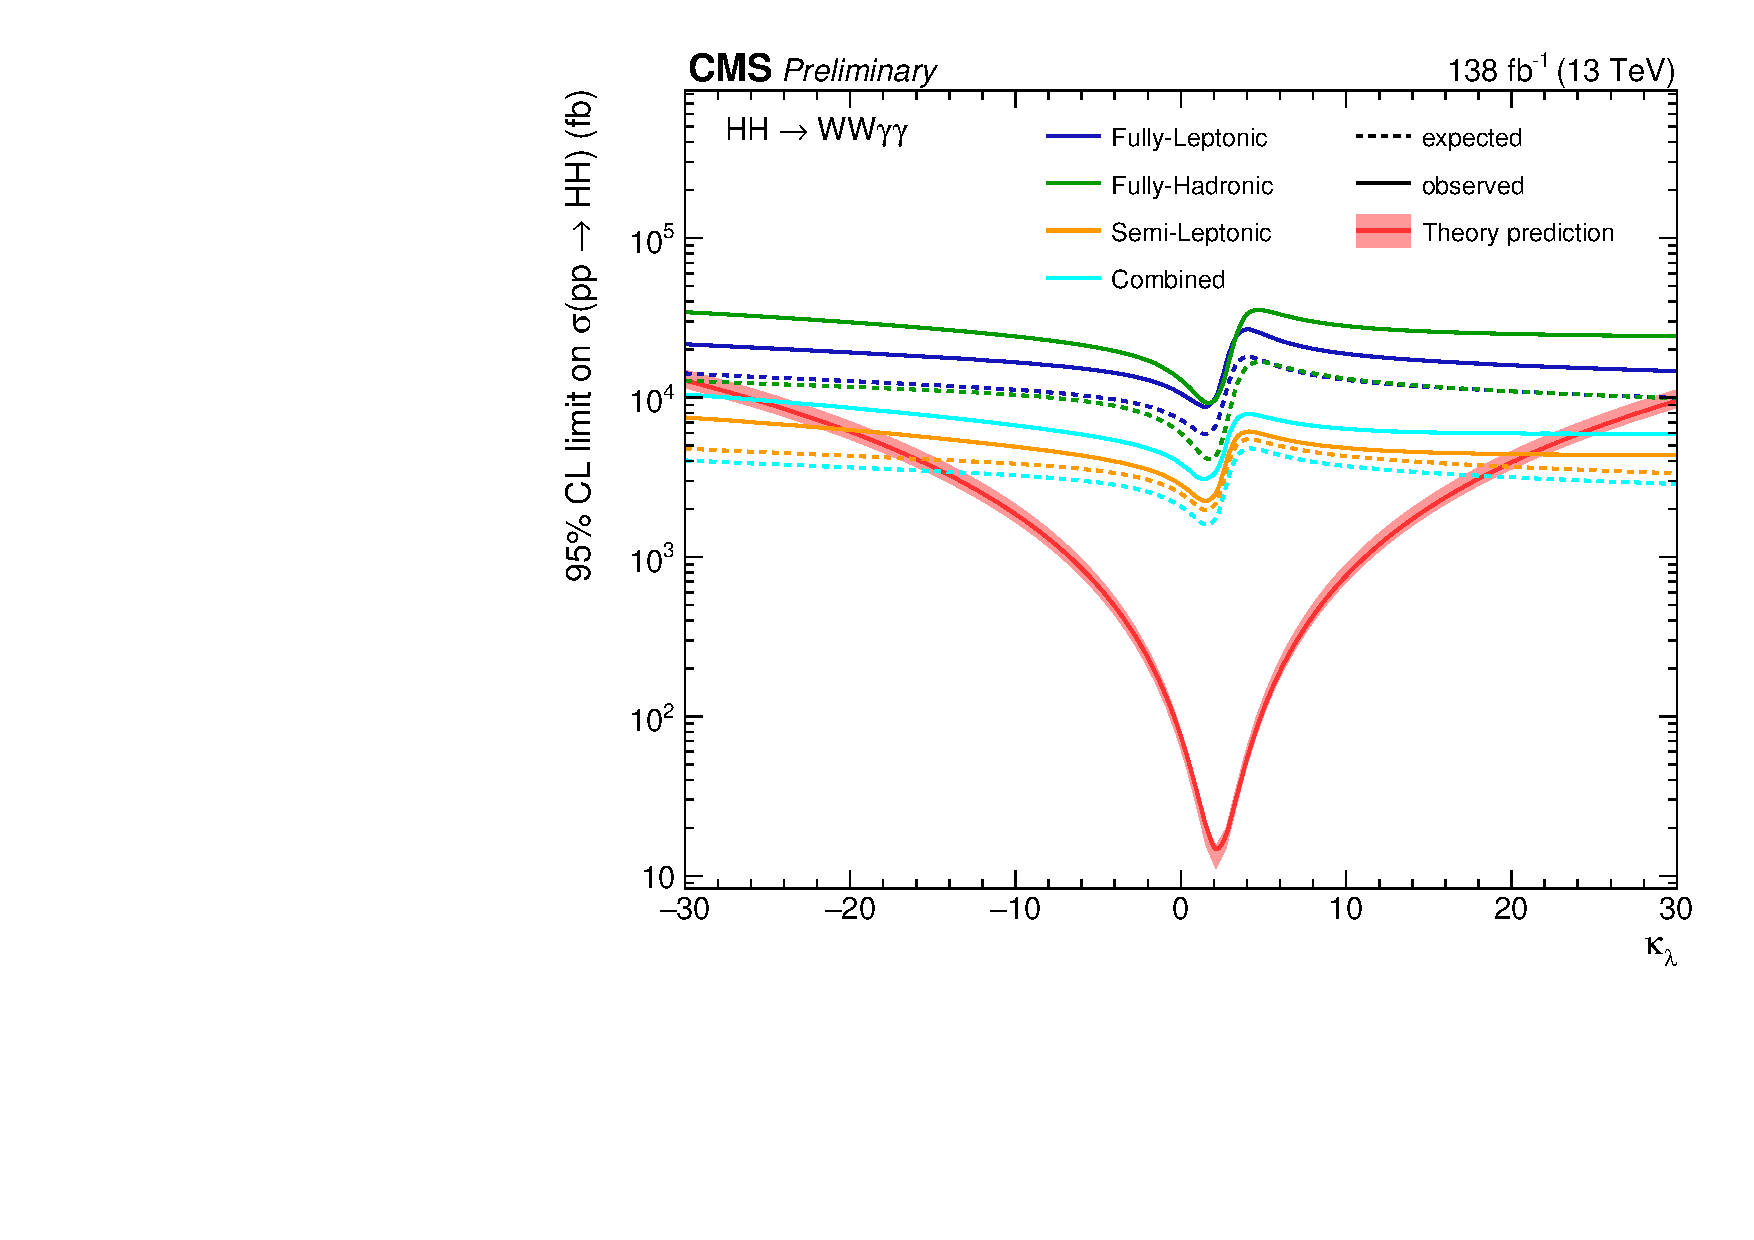
\includegraphics[width=0.45\textwidth]{Images/Results/kl_Comparison.pdf} \label{fig:Channel_kl}} 
  \qquad
  \subfloat[Combined]{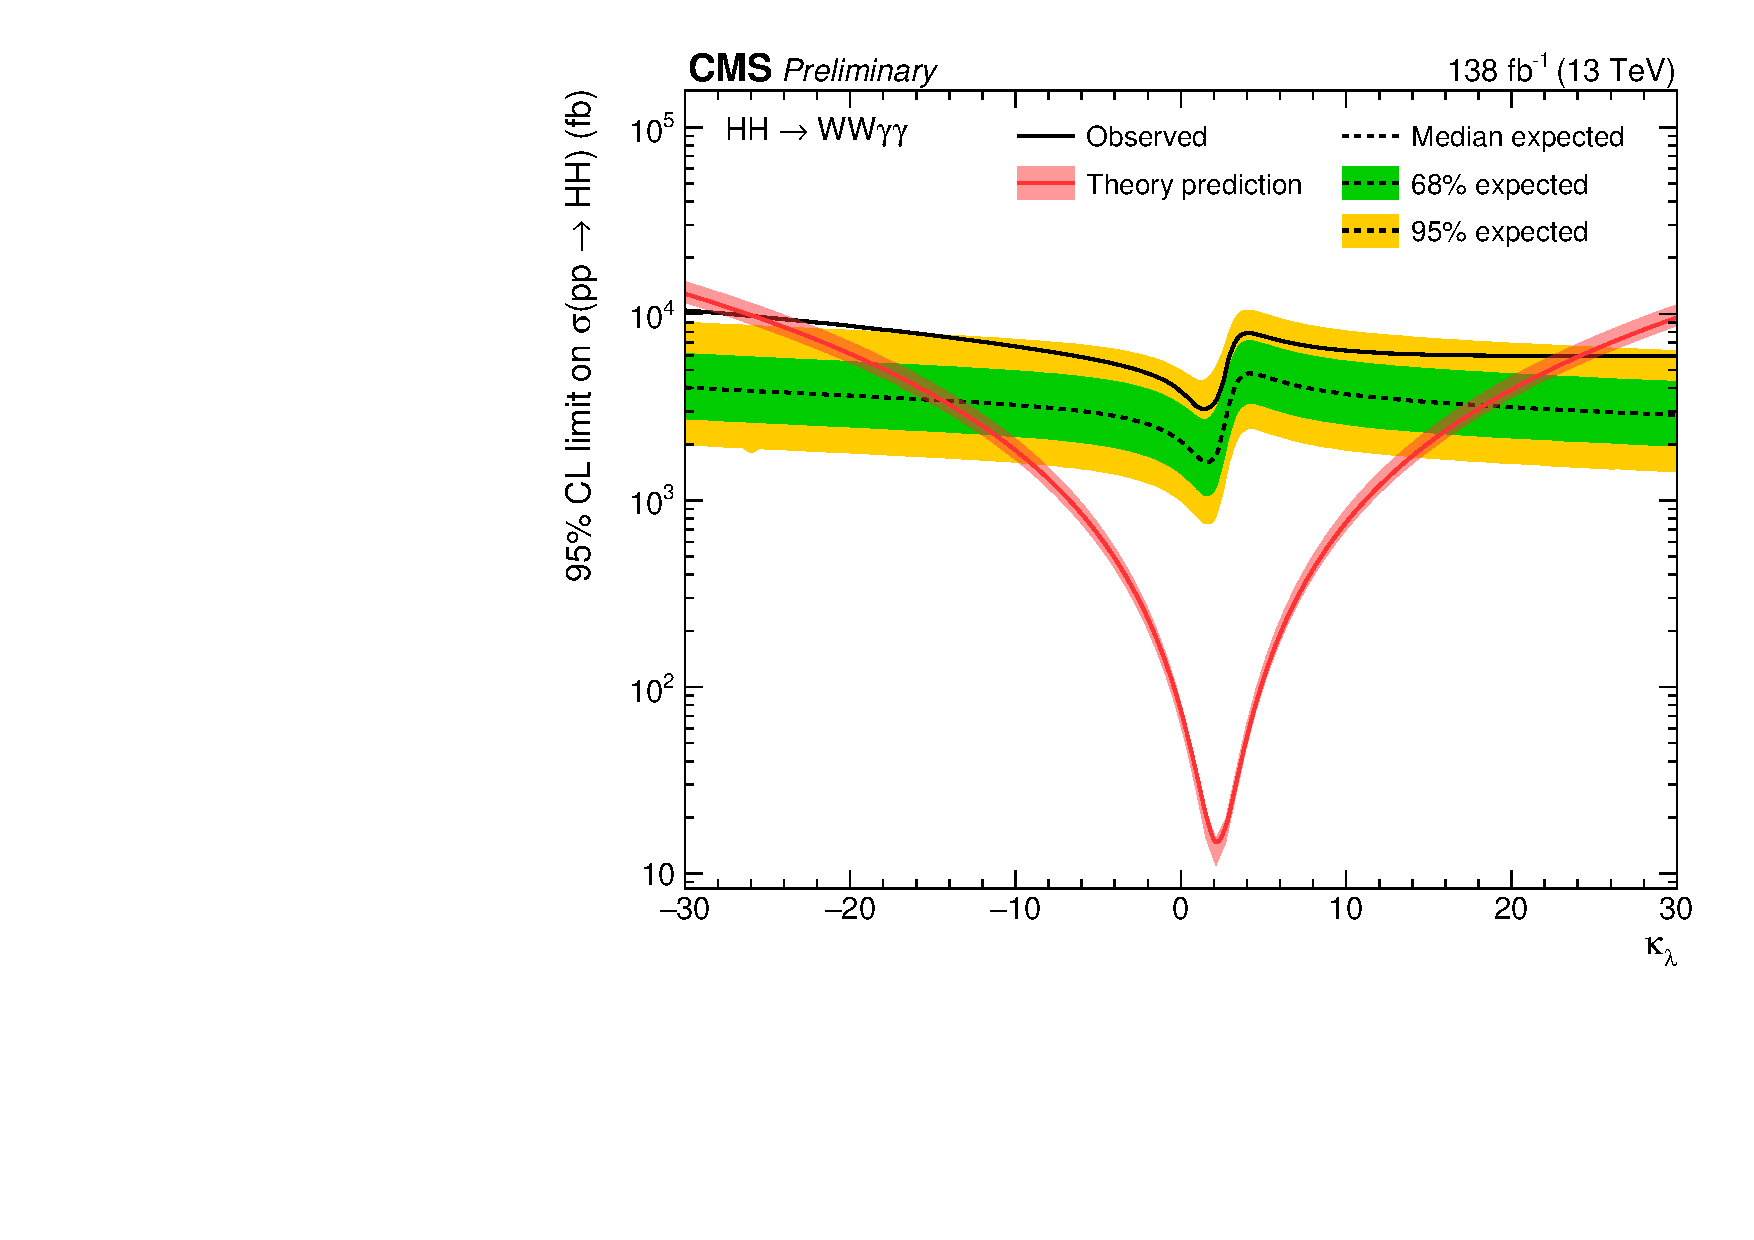
\includegraphics[width=0.45\textwidth]{Images/Results/HHWWgg_kl_Scan.pdf}\label{fig:Combined_kl}}
  \caption{95\% $CL_{s}$ upper limit scan of $\kappa_{\lambda}$ hypotheses from -30 to 30.}
  \label{fig:kl_scan}
\end{figure}

\begin{figure}[!htbp]
  \setcounter{subfigure}{0}
  \centering
  \subfloat[Per channel]{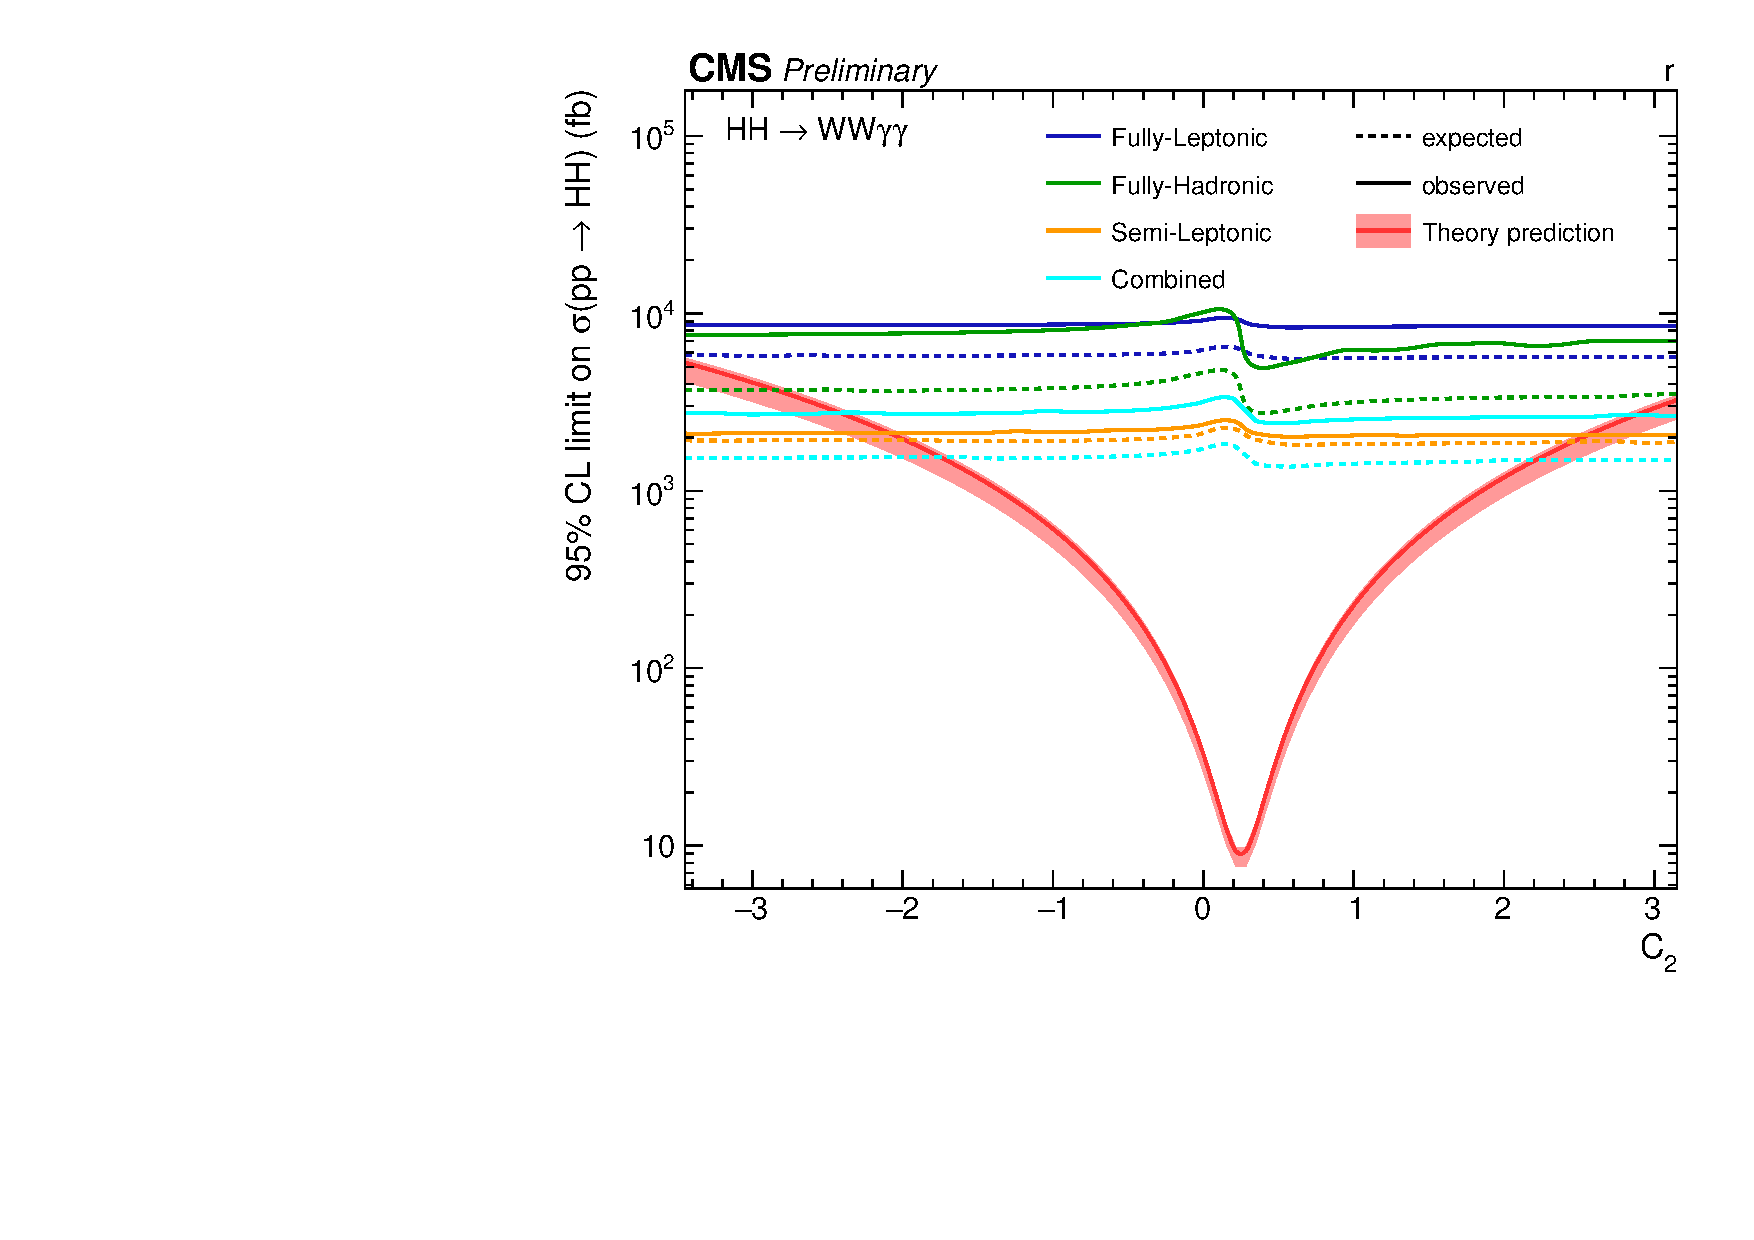
\includegraphics[width=0.45\textwidth]{Images/Results/C2_Comparison.pdf}\label{fig:Channel_c2}} 
  \qquad
  \subfloat[Combined]{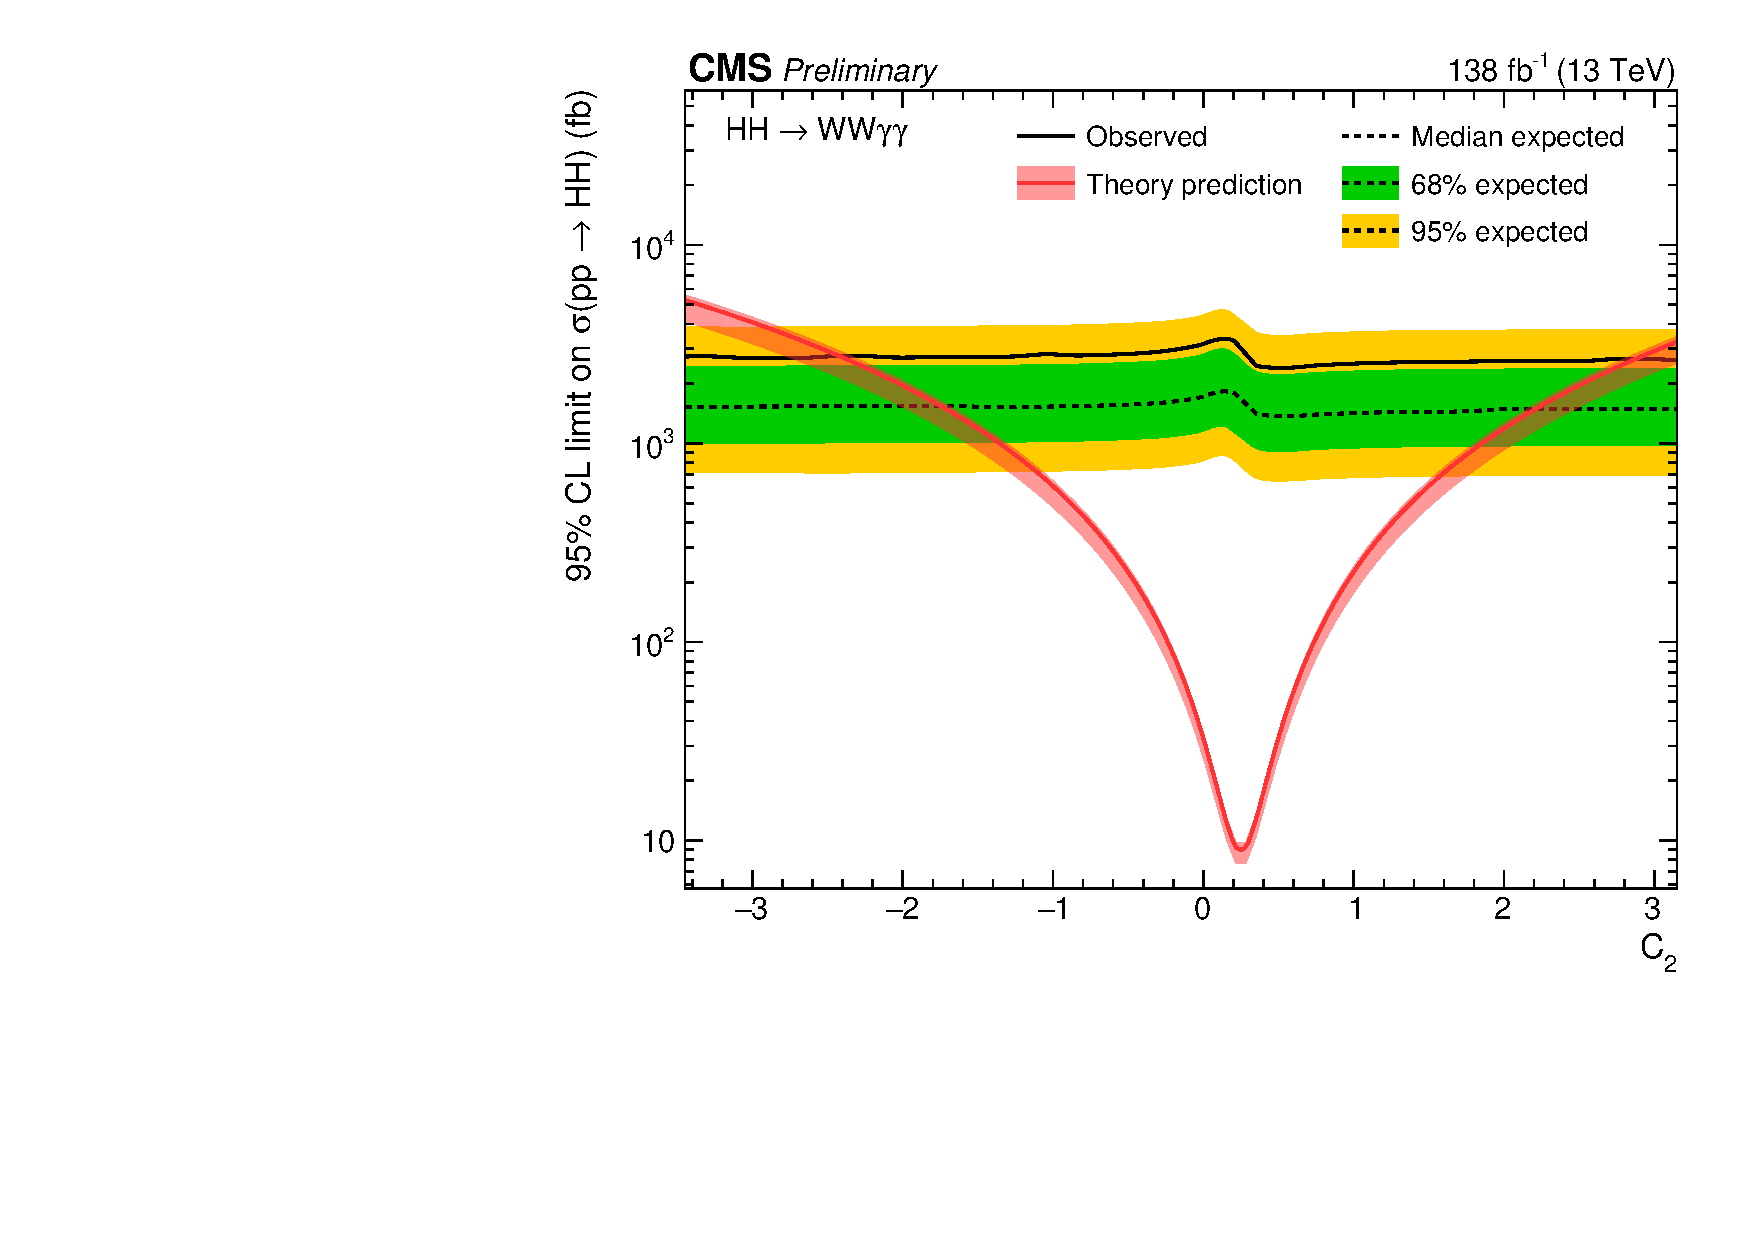
\includegraphics[width=0.45\textwidth]{Images/Results/HHWWgg_C2_Scan.pdf}\label{fig:Combined_c2}}
  \caption{95\% $CL_{s}$ upper limit scan of $c_{2}$ hypotheses from -3 to 3.}
  \label{fig:c2_scan}
\end{figure}

\begin{figure}[!htbp]
\centering
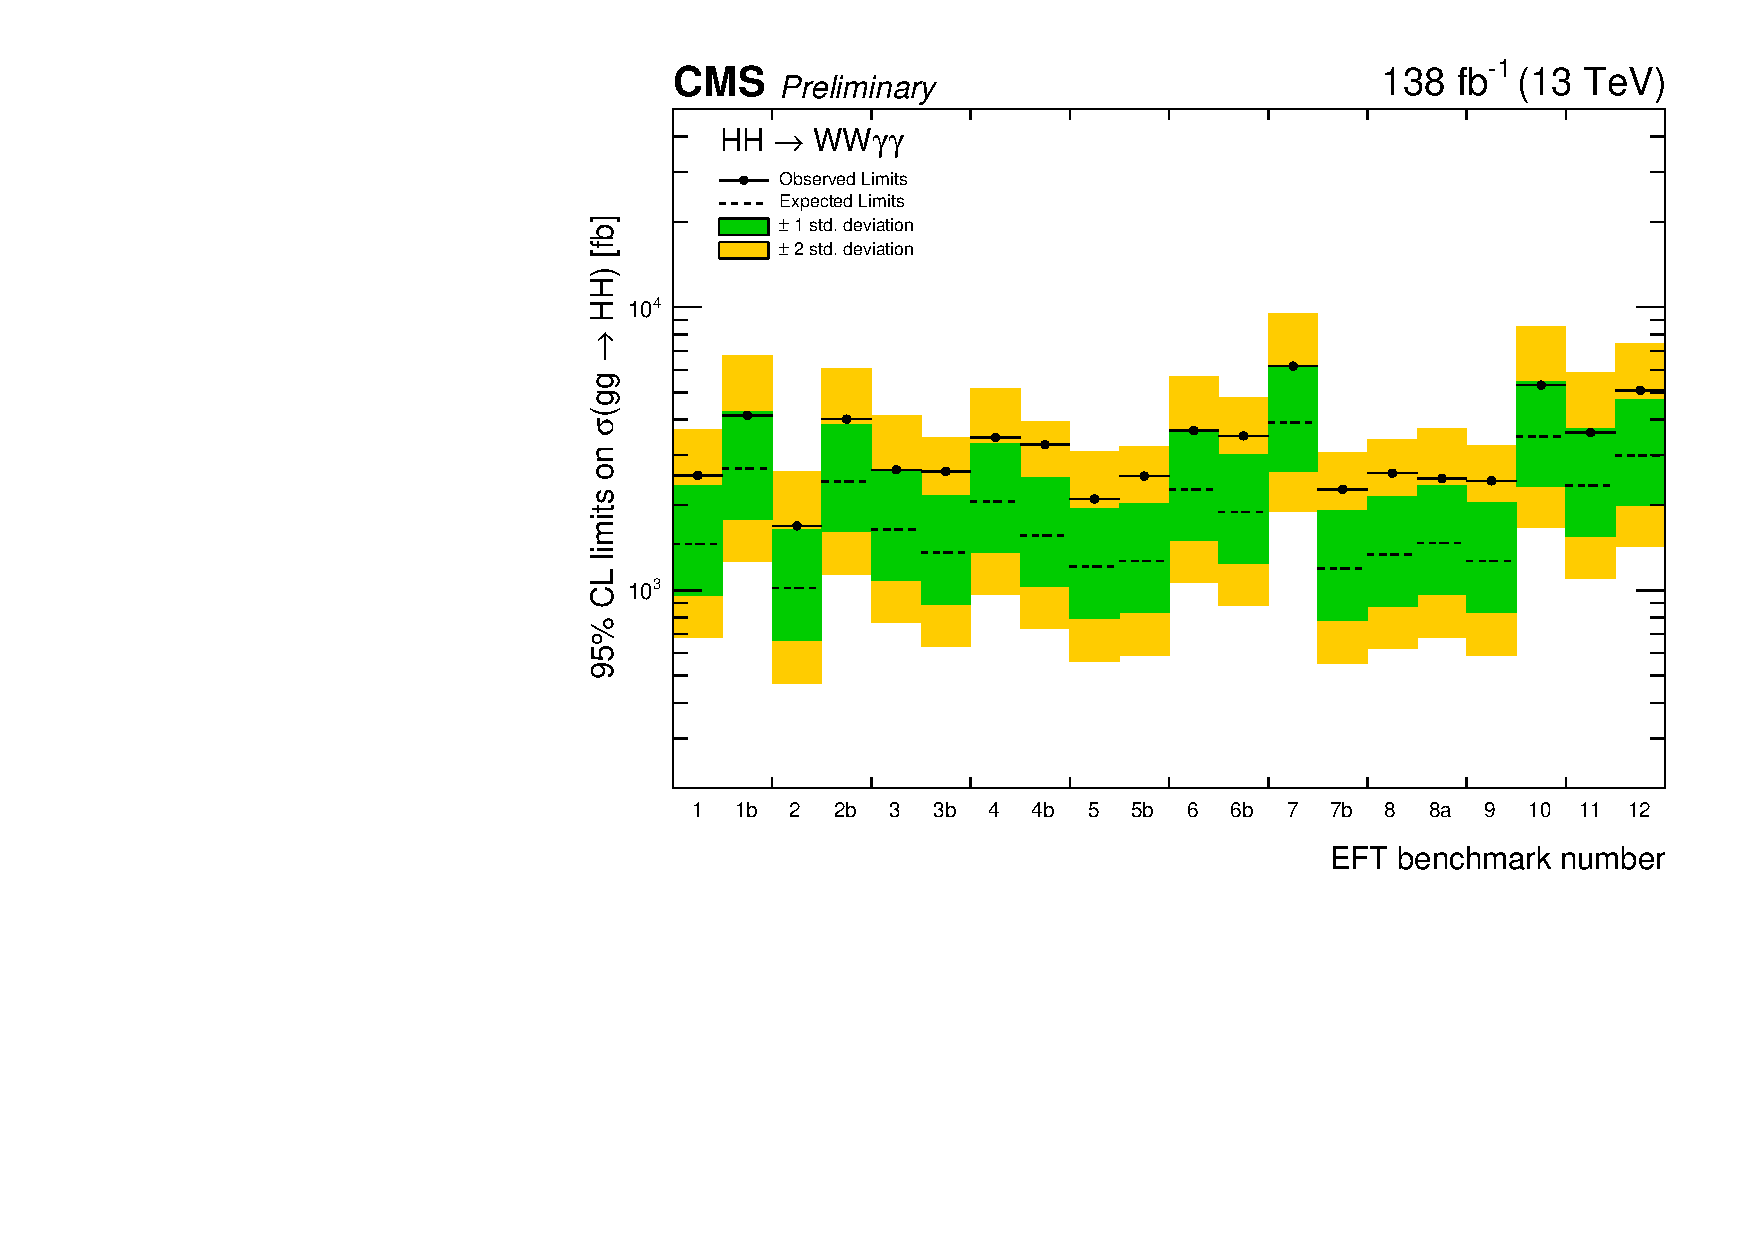
\includegraphics[width=0.75\textwidth]{Images/Results/EFT_CombinedUpperlimits.pdf}
\caption{Run 2 95\% $CL_{s}$ limits on HH gluon gluon fusion production for different nonresonant benchmark models defined in Table \ref{tab:eft_bench}.}
\label{fig:20_EFT_benchmark_results_all}
\end{figure}

\section{Summary} \label{section:Summary}

In this article, the first search for Higgs pair production in the WW$\gamma\gamma$ final state performed by the CMS collaboration has been presented. The analysis makes use of 
data collected with the CMS detector between 2016 and 2018 corresponding to an integrated luminosity of 138 \unit{fb}$^{-1}$, from proton-proton collisions at a center-of-mass energy of 13 TeV.
Combining all final state categories, which makes use of all three WW decay modes, results in an observed (expected) 95\% $CL_{s}$ upper limit on the di-Higgs production cross-section of 
3.0 (1.7) pb, corresponding to about 97 (53) times the standard model prediction. Scans of modified SM and purely BSM coupling parameters in an EFT framework result in an
observed (expected) constraint on the Higgs self-coupling of -25.9 (-14.5) to 24.1 (18.4) times its standard model value, and a constraint on the magnitude of the 
direct coupling of two top quarks to two Higgs bosons of -2.4 (-1.7) to 2.9 (2.2) at a 95\% $CL_{s}$. Additionally, observed (expected) 95\% $CL_{s}$ upper limits are 
placed on twenty EFT benchmark scenarios ranging from 1.7 - 6.2 (1.0 - 3.9) pb.

\chapter{Resonant production of HH}
% % % % 
\chapter{Differential and Fiducial Cross-section measurement}

\section{Introduction} \label{sec:intro}
% In 2012 the ATLAS and CMS collaborations announced the discovery of a new particle~\cite{Aad:2012tfa,Chatrchyan:2012ufa,Chatrchyan:2013lba} and subsequent measurements of its properties~\cite{ATLASPropertiesRun1,CMSPropertiesRun1,ATLASCMSMassRun1,ATLASCMSPropertiesRun1} confirmed it to be consistent with the standard model (SM) expectations for the Higgs (\PH) boson, setting a major breakthrough in the understanding of the electroweak symmetry breaking mechanism~\cite{Englert:1964et,Higgs:1964ia,Higgs:1964pj,Guralnik:1964eu,Higgs:1966ev,Kibble:1967sv}.

The large signal-to-background ratio and the completely resolved final state characteristic of the $\HZZfl$ decay channel ($\ell=\Pe,\Pgm$) identify it as one of the pillars to probe the SM predictions and to measure the properties of the \PH boson.
An extensive set of measurements has been performed using this decay channel bot with the LHC Run 1 data set at center-of-mass energies of 7 and 8\TeV, and the Run 2 data set at 13\TeV, including the determination of
the mass, the spin and the parity of the \PH boson~\cite{ATLASH4lLegacyRun1,CMSH4lLegacyRun1,CMSH4lSpinParity,CMSH4lAnomalousCouplings,CMSH4l2016,ATLASH4l2016},
its width~\cite{CMSH4lWidth,CMSH4lLifetime,ATLASH4lWidth,ATLASH4lWidth2016}, the inclusive and differential fiducial cross sections~\cite{ATLASH4lFiducial8TeV,CMSH4lFiducial8TeV, CMSH4l2016,ATLASH4lFiducial2016, ATLASH4lLegacyRun2, ATLASH4lFiducialRun2}, and the tensor structure of the \PH boson interaction with a pair of neutral gauge bosons in both on-shell and off-shell regions~\cite{CMSH4lAnomalousCouplings,CMSH4lLifetime, CMSH4lAnomalousCouplings2016,ATLASH4l2016,CMSHVVAnomalousCouplings2016}.

This chapter presents the measurements of the integrated and differential cross sections of the \PH boson in the $\HZZfl$ decay channel using data from proton-proton ($\Pp\Pp$) collisions at a center-of-mass energy of $\sqrt{s}=13\TeV$, collected by the CMS detector at the LHC and corresponding to an integrated luminosity of $\usedLumiABC$. 
All the measurements are performed within a ``fiducial'' phase space region defined to closely reproduce the experimental acceptance and the reconstruction level selection.
This approach is chosen to enhance the model independence of the results and to reduce the systematic uncertainties associated to the cross sections determination.

The differential cross sections are measured for several kinematic observables sesitive to either the production or the decay sides of the $\HZZfl$ process, therefore providing a complete characterization of its properties and a full coverage of the entire fiducial phase space.
In order to probe the SM predictions against alternative BSM scenarios, we perform differential cross section measurements in bins of matrix element kinematic discriminants sensitive to the $\HZZfl$ decay.
Additional double differential measurements, where the cross section is extracted within bins defined by complementary kinematic cuts on two observables, are also presented. 

The analysis strategy employed reflects the one used in previous measurements of the \PH boson properties in the four lepton channel \cite{CMSH4lFiducial8TeV, CMSHIG19001}.

This chapter is organized as follows. 
The data set used for the analysis is presented in Section~\ref{sec:samples}, along with a description of the simulated signal and background samples.
The event reconstruction techniques and the selection algorithm used to identify the \PH boson candidates are outlined in Section~\ref{sec:reconstruction}.
The definition of the restricted phase space region where the differential cross sections are measured is given in Section~\ref{sec:fiducialvolume}.
A complete description of all the kinematic observables used in the analysis is presented in Section~\ref{sec:observables}, with a particular focus on the construction of matrix element kinematic discriminants in Section~\ref{sec:discriminants}.
The background and signal modelling are presented in Section~\ref{sec:bkgd} and \ref{sec:signal}, respectively.
The statistical procedure adopted in the extraction of the integrated and differential cross sections is presented in Section~\ref{sec:measurement}. 
The different sources of systematic uncertainty that enter the analysis are discussed in Section~\ref{sec:systematics}.
The results of the measurements are outlined in Section~\ref{sec:results}, along with their comparison to the SM expectations.
A summary highlighting the main findings of the analysis is given in Section~\ref{sec:summary}.

% \section{The CMS detector}
% \label{sec:detector}
% The central feature of the CMS apparatus is a superconducting solenoid of 6\unit{m} internal diameter, providing a magnetic field of 3.8\unit{T}. Within the solenoid volume are a silicon pixel and strip tracker, a lead tungstate crystal electromagnetic calorimeter (ECAL), and a brass and scintillator hadron calorimeter (HCAL), each composed of a barrel and two endcap sections. Forward calorimeters extend the pseudorapidity coverage provided by the barrel and endcap detectors. Muons are detected in gas-ionization chambers embedded in the steel flux-return yoke outside the solenoid. The electromagnetic calorimeter consists of 75\,848 lead tungstate crystals, which provide coverage in pseudorapidity $\abs{\eta} < 1.48 $ in a barrel region (EB) and $1.48 < \abs{\eta} < 3.0$ in two endcap regions (EE). Preshower detectors consisting of two planes of silicon sensors interleaved with a total of $3 X_0$ of lead are located in front of each EE detector. The forward hadron (HF) calorimeter uses steel as an absorber and quartz fibers as the sensitive material. The two halves of the HF are located 11.2\unit{m} from the interaction region, one on each end, and together they provide coverage in the range $3.0 < \abs{\eta} < 5.2$. They also serve as luminosity monitors. 

% Events of interest are selected using a two-tiered trigger system. The first level (L1), composed of custom hardware processors, uses information from the calorimeters and muon detectors to select events at a rate of around 100\unit{kHz} within a fixed latency of about 4\mus~\cite{Sirunyan:2020zal}. The second level, known as the high-level trigger (HLT), consists of a farm of processors running a version of the full event reconstruction software optimized for fast processing, and reduces the event rate to around 1\unit{kHz} before data storage~\cite{Khachatryan:2016bia}. 

% The candidate vertex with the largest value of summed physics-object $\pt^2$ is taken to be the primary $\Pp\Pp$ interaction vertex. The physics objects are the jets, clustered using the jet finding algorithm~\cite{Cacciari:2008gp,Cacciari:2011ma} with the tracks assigned to candidate vertices as inputs, and the associated missing transverse momentum, taken as the negative vector sum of the \pt of those jets. More details are given in Section~9.4.1 of Ref.~\cite{CMS-TDR-15-02}.

% The electron momentum is estimated by combining the energy measurement in the ECAL with the momentum measurement in the tracker. The momentum resolution for electrons with $\pt \approx 45\GeV$ from $\Z \rightarrow \Pe \Pe$ decays ranges from 1.7\% to 4.5\%. It is generally better in the barrel region than in the endcaps, and also depends on the bremsstrahlung energy emitted by the electron as it traverses the material in front of the ECAL~\cite{Khachatryan:2015hwa}.

% Muons are measured in the pseudorapidity range $\abs{\eta} < 2.4$, with detection planes made using three technologies: drift tubes, cathode strip chambers, and resistive plate chambers. The single muon trigger efficiency exceeds 90\% over the full $\eta$ range, and the efficiency to reconstruct and identify muons is greater than 96\%. Matching muons to tracks measured in the silicon tracker results in a relative transverse momentum resolution, for muons with \pt up to 100\GeV, of 1\% in the barrel and 3\% in the endcaps. The \pt resolution in the barrel is better than 7\% for muons with \pt up to 1\TeV~\cite{Sirunyan:2018}. 

% A more detailed description of the CMS detector, together with a definition of the coordinate system used and the relevant kinematic variables, can be found in Ref.~\cite{Chatrchyan:2008zzk}. 

\section{Data and simulated samples}
\label{sec:samples}
The results presented in this paper are obtained from the analysis of the proton-proton collisions recorded at $\sqrt{s}=13\TeV$ by the CMS experiment at the LHC in 2016, 2017, and 2018. The integrated luminosities of the three data taking periods are 36.3, 41.8, and 59.8\fbinv, for a total of about 138\fbinv of data analysed~\cite{CMS-PAS-LUM-17-001,CMS-PAS-LUM-17-004,CMS-PAS-LUM-18-002}.

Candidates are selected among leptons passing loose identification and isolation requirements using di-electron, di-muon, and electron-muon high level trigger algorithms. The different \pt thresholds for each data taking period are reported in Tab.~\ref{tab:HLT}. A maximal coverage of the $\HZZfl$ phase space is ensured from additional triggers requiring three leptons with loose \pt thresholds and no isolation criteria, as well as single-electron and single-muon triggers.
The collection of $4\ell$ events selected from the single-lepton triggers is used to measure the trigger efficiency by means of a ``tag and probe'' technique. A ``tag'' lepton is defined as such if it matches geometrically a candidate from the single-lepton triggers, whilst the other leptons are used as ``probes'' and are combined together to reconstruct any of the triggers adopted in the analysis. The trigger efficiency measured on simulated samples is found to be larger than 99\%, in a good agreement with the corresponding value for data.

\begin{table}[htb]
	\centering
	\topcaption{
% 		\textbf{To Edit:}
		The minimal \pt of the leading/subleading leptons for the main di-electron (\Pe/\Pe), di-muon (\Pgm/\Pgm), and electron-muon (\Pe/\Pgm, \Pgm/\Pe) high-level trigger algorithms used in the $\Hllll$ analysis in 2016, 2017, and 2018.
		\label{tab:HLT}
	}
	\begin{tabular}{cccc}
		& \Pe/\Pe ({\GeVns}) & \Pgm/\Pgm ({\GeVns})& \Pe/\Pgm, \Pgm/\Pe ({\GeVns})\\
		\hline
		2016 & 17/12 & 17/8 & 17/8, 8/23 \\
		2017 & 23/12 & 17/8 & 23/8, 12/23 \\
		2018 & 23/12 & 17/8 & 23/8, 12/23
	\end{tabular}
\end{table}

{\tolerance=800 
Signal samples for the five main production mechanisms of the SM \PH boson are simulated at next-to-leading order (NLO) in perturbative QCD (pQCD) with the \POWHEG~2.0~\cite{Nason:2004rx,Frixione:2007vw,Alioli:2010xd} generator. Specific tunings are used for the gluon fusion ($\ggH$)~\cite{Alioli:2008tz},
vector boson fusion ($\VBF$)~\cite{Nason:2009ai},
associated production with a vector boson ($\VH$, where \PV is a \PW or a \PZ boson)~\cite{Luisoni2013},
and associated production with a pair of top quarks ($\ttH$)~\cite{Hartanto:2015uka}. Events produced via the $\ggH$ mechanism are reweighted as a function of the transverse momentum of the \PH boson and of the number of jets in the event, to match the \textsc{NNLOPS} predictions \cite{Hamilton:2013fea}. The $\Pg\Pg\to\ZH$ contribution to the $\ZH$ production mode is simulated at leading order (LO) using \textsc{jhugen}~7.3.0~\cite{Gao:2010qx, Bolognesi:2012mm,Anderson:2013afp,Gritsan:2016hjl,Gritsan:2020pib}.
The production of the SM \PH boson in association with a single top quark ($\tH$) and either a quark ($\tHq$) or a $\PW$ boson ($\tHW$) are also considered in the analysis and simulated at LO using using \textsc{jhugen}~7.0.2 and \MGvATNLO~2.2.2~\cite{amcatnlo}, respectively.
The associated production with a pair of bottom quarks ($\bbH$) is simulated at LO with \textsc{jhugen}~7.0.2.
In all cases, the decay of the \PH boson to four leptons is modeled with \textsc{jhugen}~7.0.2.
The simulation of the different production and decay modes are based on the theoretical predictions from Refs.~\cite{Anastasiou:2015ema,Anastasiou2016,Ciccolini:2007jr,Ciccolini:2007ec,Bolzoni:2010xr,Bolzoni:2011cu,Brein:2003wg,Ciccolini:2003jy,Beenakker:2001rj,Beenakker:2002nc,Dawson:2002tg,Dawson:2003zu,Yu:2014cka,Frixione:2014qaa,Demartin:2015uha,Demartin:2016axk,Denner:2011mq,Djouadi:1997yw,hdecay2,Bredenstein:2006rh,Bredenstein:2006ha,Boselli:2015aha,Actis:2008ts} and are summarized in Ref.~\cite{deFlorian:2016spz}.\par}

{\tolerance=5000 The dominant sources of background in this analysis are the quark-antiquark annihilation and gluon fusion productions of $\PZ\PZ$ events. The former is simulated at NLO pQCD with \POWHEG~2.0~\cite{Melia:2011tj}, while the latter is generated at LO with \MCFM~7.0.1~\cite{MCFM}.
Rare background processes such as $\PW\PZ$ and the triboson productions $\PZ\PZ\PZ$, $\PW\PZ\PZ$, and $\PW\PW\PZ$ are also considered in the analysis and are modeled at NLO using \MGvATNLO~2.4.2.
The background contributions of $\ttZ$, $\ttWW$, and $\ttZZ$ processes are simulated at LO with \MGvATNLO~2.4.2.
Two dedicated data driven techniques are emploied to estimate the contributions of the reducible background events arising from $\PZ$ bosons with associated jets ($\PZ+$jets),  as described in Section~\ref{sec:redbkgd}.\par}
%The events containing $\PZ$ bosons with associated jets ($\PZ+$jets) are simulated at NLO with \MGvATNLO~2.4.2 and the $\ttbar$ background is simulated at NNLO with \POWHEG~2.0.
%The reducible background determination does not rely on the MC but is based on data, as described in Section~\ref{sec:redbkgd}.\par}

To simulate the parton showering and hadronization effects all the MC generators are interfaced with \PYTHIA 8.230~\cite{Sjostrand:2014zea} using the CUETP8M1 tune~\cite{Khachatryan:2015pea} for the 2016 data-taking period and the CP5 tune~\cite{Sirunyan:2019dfx} for the 2017 and 2018 data-taking periods. Parton distribution functions (PDFs) are taken from the NNPDF3.0 set \cite{Ball:2014uwa} for all three data taking periods.

Although not directly used to model any process, an additional sample of Drell-Yann with jets events is produced with \MGvATNLO~2.4.2 for validation studies and for the training of the Boosted Decision Tree (BDT) used for the identification and isolation of electrons, as described in Section~\ref{sec:reconstruction}.

In order to simulate the response of the CMS detector a dedicated modelling based on the \GEANTfour~\cite{Agostinelli:2002hh,GEANT} package is used. The simulated events are reconstructed with the same algorithms used for data and are reweighted in such a way that the distribution of pileup events per bunch crossing matches the one observed in data.

\section{Event reconstruction and selection}
\label{sec:reconstruction}
% The particle-flow algorithm~\cite{CMS-PRF-14-001} aims to reconstruct and identify each individual particle in an event, with an optimized combination of information from the various elements of the CMS detector. The energy of photons is obtained from the ECAL measurement. The energy of electrons is determined from a combination of the electron momentum at the primary interaction vertex as determined by the tracker, the energy of the corresponding ECAL cluster, and the energy sum of all bremsstrahlung photons spatially compatible with originating from the electron track. The energy of muons is obtained from the curvature of the corresponding track. The energy of charged hadrons is determined from a combination of their momentum measured in the tracker and the matching ECAL and HCAL energy deposits, corrected for the response function of the calorimeters to hadronic showers. Finally, the energy of neutral hadrons is obtained from the corresponding corrected ECAL and HCAL energies.

%% Probably can be removed, as pTmiss is not used in the analysis
% 23/05: Leave out, does not bring additional information.
%The missing transverse momentum vector \ptvecmiss is computed as the negative vector sum of the transverse momenta of all the PF candidates in an event, and its magnitude is denoted as \ptmiss~\cite{Sirunyan:2019kia}. The \ptvecmiss is modified to account for corrections to the energy scale of the reconstructed jets in the event. 

% The information from the silicon tracker and the muon system~\cite{Sirunyan:2018} is combined to reconstruct muons with $\pt^{\Pgm} > 5\GeV$ and $\abs{\eta^{\Pgm}} < 2.4$. 
% Both tracks from the silicon trackers and from the muon system can be used as seeds for the matching between inner and outer tracks. 
% Cases where inner tracks are matched to segments in only one or two muons stations are also considered to cope with situations of very low-\pt muons that do not traverse the entire detector. 
% Loose requirements on the muons track candidates in the muon system and the inner tracker are used, taking into account their compatibility with small energy deposits in the ECAL and HCAL, to define the muon objects considered in the analysis.

% An additional isolation requirement of ${\mathcal I}^{\Pgm}$ is introduced to discriminate between muons \PZ boson decay and those originating from electroweak (EW) decays of hadrons within jets:

% \begin{linenomath}
% 	\ifthenelse{\boolean{cms@external}}
% 	{
% 		\begin{multline}
% 		\label{eqn:pfiso}
% 		{\mathcal I}^{\Pgm} \equiv \Big( \sum \pt^\text{charged} + \max\big[ 0, \sum \pt^\text{neutral} +\\
% 		\sum \pt^{\Pgg} - \pt^{\Pgm,\mathrm{PU}} \big] \Big) / \pt^{\Pgm} .
% 		\end{multline}
% 	}
% 	{
% 		\begin{equation}
% 		\label{eqn:pfiso}
% 		{\mathcal I}^{\Pgm} \equiv \Big( \sum \pt^\text{charged} + \max\big[ 0, \sum \pt^\text{neutral} +
% 		\sum \pt^{\Pgg} - \pt^{\Pgm,\mathrm{PU}} \big] \Big) / \pt^{\Pgm} .
% 		\end{equation}
% 	}
% \end{linenomath}

% {\tolerance=800 A relative isolation of ${\mathcal I}^{\Pgm}<0.35$ is imposed in the analysis. The quantity $\sum \pt^\text{charged}$ represents the scalar sum of the transverse momenta of charge hadrons originating from the primary vertex (PV) selected in the event, while $\sum \pt^\text{neutral}$ and $\sum \pt^{\Pgg}$ define the corresponding scalar sums for neutral hadrons and photons, respectively.
% The isolation requirement is defined within a cone of angular radius $\Delta R=0.3$ around the muon direction at the PV, with the angular distance between two particles $i$ and $j$ defined as $\Delta R(i,j) = \sqrt{\smash[b]{(\eta^i-\eta^j)^{2} + (\phi^i-\phi^j)^{2}}}$.
% The quantity $\pt^{\Pgm,\mathrm{PU}}$ in Eq.~(\ref{eqn:pfiso}) is defined as $\pt^{\Pgm,\mathrm{PU}}\equiv0.5\sum_{i}\pt^\text{\textit{i},PU}$, from the sum of the transvers momenta of all the charged hadrons $i$ originating from the PV corrected for the different fraction of charged and neutral particles in the cone~\cite{PUmitigationCMS} by the 0.5 factor. The $\pt^{\Pgm,\mathrm{PU}}$ contribution is subtracted from ${\mathcal I}^{\Pgm}$ to correct for energy deposits arising from pileup interactions.\par}

% {\tolerance=1200 The information from the ECAL and the tracker is combined to reconstruct electrons~\cite{EGM-17-001} within the geometrical acceptance of the detector, defined by the pseudorapidity region $\abs{\eta^{\Pe}} < 2.5$, and with $\pt^{\Pe} > 7\GeV$.
% The idenfitication of electrons is performed with a BDT algorithm sensitive to the presence of bremsstrahlung along the electron trajectory, the geometrical and momentum-energy matching between the
% electron trajectory and the corresponding cluster in the ECAL, the features of the electromagnetic shower in the ECAL,
% and observables that discriminate against electrons originating from photon conversions.
% Conversly to muons, where the isolation of the PF candidates is performed with the ${\mathcal I}^{\Pgm}$ requirement aforementioned, the isolation sums for electrons are included in the BDT discriminant.
% This choice is proven to enhance the suppression of electrons originating from electroweak decays of hadrons within jets~\cite{DPS-2018} and has a better performance than a cut-based approach on the relative isolation observable.
% The BDT for the identification and isolation of electrons is developed within the \textsc{xgboost}~\cite{Chen:2016btl} library.
% The training is performed on dedicated Drell-Yann + jets simulated events that are not used elsewhere in the analysis in six mutually exclusive regions defined by two transverse momentum (7$<\pt^{\Pe}<$10$\GeV$ and $\pt^{\Pe}>$10$\GeV$) and three pseudorapidity cuts corresponding to the central barrel ($\abs{\eta^{\Pe}}<0.8$), outer barrel ($0.8<\abs{\eta^{\Pe}}<1.479$), and endcaps ($1.479<\abs{\eta^{\Pe}}<2.5$).
% The BDT is trained separately on the three data-taking periods and the selection requirements are defined by requiring the same signal efficiency for all three periods.\par}

The objects electrons, photons, muons and jets are selected as described in Section~\ref{sec:4}.

% The \ref{sec:4}

Final-state radiation (FSR) photons emitted by $\PZ\rightarrow \ell^+\ell^-$ are taken into account for an optimal reconstruction of the $\PH\rightarrow4\ell$ decay. More precisely, PF photon candidates with $\abs{\eta^\Pgg}<2.4$ are considered as FSR objects if they have transverse momentum $\pt^{\Pgg} > 2 \GeV$ and relative isolation factor ${\mathcal I}^{\Pgg} <1.8$, where ${\mathcal I}^{\Pgg}$ is defined as of Eq.~(\ref{eqn:pfiso}) for muons.
These FSR candidates are associated to the the closest selected lepton in the event and are not retained in the analysis if $\Delta R(\Pgg,\ell)/(\pt^{\Pgg})^2>0.012 \GeV^{-2}$ and $\Delta R(\Pgg,\ell) > 0.5$.
For evey lepton, the FSR candidate with the lowest-$\Delta R(\Pgg,\ell)/(\pt^{\Pgg})^2$, if any, is considered.
The photons candidates identified from the FSR recovery algorithm are excluded from the computation of the isolation factor of the muons selected in the event.

Leptons with a ratio of their impact parameter in three dimenstions, computed with respect to the position of the PV selected, to their uncertainty grater or equal to four are rejected to enhance the suppression of muons from in-flight decays of hadrons and electrons from photon conversions.

The decay products of known dilepton resonances are used to calibrate the momentum scale and resolution of electrons and muons in bins of $\pt^{\ell}$ and $\eta^{\ell}$, as described in Refs.~\cite{EGM-17-001,Sirunyan:2018}.

The efficiency of the reconstruction and selection from prompt leptons is measured in several bins of $\pt^{\ell}$ and $\eta^{\ell}$ by means of a ``tag and probe'' technique~\cite{CMS:2011aa} using samples of $\PZ$ boson events both in data and simulation. The yields of selected events in simulated samples are rescaled by the difference in efficiencies measured in simulation and data.

% For each event, hadronic jets are clustered from these reconstructed particles using the infrared and collinear safe anti-\kt algorithm~\cite{Cacciari:2008gp, Cacciari:2011ma} with a distance parameter of 0.4. The jet momentum is determined as the vectorial sum of all particle momenta in the jet, and is found from simulation to be, on average, within 5 to 10\% of the true momentum over the whole \pt spectrum and detector acceptance. Additional proton-proton interactions within the same or nearby bunch crossings can contribute additional tracks and calorimetric energy depositions, increasing the apparent jet momentum. To mitigate this effect, tracks identified to be originating from pileup vertices are discarded and an offset correction is applied to correct for remaining contributions. Jet energy corrections are derived from simulation studies so that the average measured energy of jets becomes identical to that of particle level jets. In situ measurements of the momentum balance in dijet, photon+jet, Z+jet, and multijet events are used to determine any residual differences between the jet energy scale in data and in simulation, and appropriate corrections are made~\cite{Khachatryan:2016kdb}. Additional selection criteria are applied to each jet to remove jets potentially dominated by instrumental effects or reconstruction failures. In this analysis only jets with $\pt^{\text{jet}}>30\GeV$
% and $\abs{\eta^{\text{jet}}} < 4.7$, and with a distance parameter of $\Delta R(\ell/\cPgg,\text{jet})>0.4$ from all selected leptons and FSR photons, are considered. Jets not satisfying the tight identification criteria and the tight working point of pileup jet identification described in Ref.~\cite{PUmitigationCMS} are discarded.

% Jets originating from {\PQqb}-quarks are tagged using the DeepCSV algorithm~\cite{Sirunyan:2017ezt}, which combines information about impact parameter significance, secondary vertex, and jet kinematics.
% Simulation samples are scaled by the difference in {\PQqb} tagging efficiency measured in simulation and data as a function of jet \pt, $\eta$, and flavor.

% The PF objects aforementioned serve as input for the analysis event selection, which targets events containing at least four well-identified and isolated leptons originating from the PV and possibly accompained by an FSR photon candidate. FSR photons are included in the invariant mass computations, unless otherwise stated.
The event selection closely follows the one employed in Ref.~\cite{CMSHIG19001} and is detailed below.
 
In the first step of the selection $\PZ$ candidates are formed from pairs of leptons of the same flavor and opposite-charge ($\Pep\Pem$, $\PGmp\PGmm$) passing the requirement $12 < \mlplm  < 120\GeV$. 
Afterwards they are merged to create $\PZ\PZ$ candidates, wherein $\PZ_1$ denotes the $\PZ$ candidate with invariant mass closest to the nominal $\PZ$ boson mass~\cite{Zyla:2020zbs}, and $\PZ_2$ the other one.
The flavors of the involved leptons define three mutually exclusive subchannels: $4\Pe$, $4\Pgm$, and $2\Pe 2\Pgm$.

A set of kinematic requirements, designed to improve the sensitivity to \PH boson decays, has to be fulfilled by the $\PZ\PZ$ candidates to be selected for the analysis.
The $\PZ_1$ candidates are required to have invariant mass larger than 40\GeV.
All the lepton pairs $\ell_i, \ell_j$ must be separated by an angular distance of at least $\Delta R(\ell_i, \ell_j) > 0.02$.
All the events selected must have two leptons with transverse momentum $\pt > 10\GeV$ and at least one with $\pt > 20\GeV$.	
In the $4\Pgm$ and $4\Pe$ subchannels, where the same four leptons can be used to build an alternative $\PZ_a \PZ_b$ candidate, candidates with $m_{\PZ_b}<12\GeV$ are not considered if $\PZ_a$ is closer to the nominal $\PZ$ boson mass than $\PZ_1$ is. This selection ensures the rejection of events with an on-shell $\PZ$ and a low-mass dilepton resonance.
The invariant mass of all the four opposite-charge lepton pairs, computed without the selected FSR photons, is required to be $m_{\ell^{+}\ell'^{-}} > 4\GeV$ in order to further suppress events with leptons originating from hadron decays in jet fragmentation or from the decay of low-mass resonances.
Eventually $\PZ\PZ$ candidates are retained for the analysis if the invariant mass of the four-lepton system $\mllll$ is larger than 70\GeV.

In events with more than one $\PZ\PZ$ candidate passes the selection requirements defined above, the one with the largest sum of transverse momenta for the two leptons defining $\PZ_2$ is retained.

Eventually, only events with $105<\mllll<160$\GeV are considered for the statistical analysis, where the mass range is chosen to be 20~GeV larger than the one used in Ref.~\cite{CMSHIG19001} to allow a measurement of the normalization of the irreducible background events using data. 

\section{Fiducial phase space definition}
\label{sec:fiducialvolume}
Differential cross sections are  measured in a fiducial phase space defined to closely match the experimental acceptance obtained with the reconstruction-level selection. 
The fiducial phase space is defined at generator-level following the same strategy adopted in previous $\PH\rightarrow4\ell$ analyses Ref.~\cite{CMSH4l2016,CMSHIG19001}. It relies on a specific set of cuts on the leptons kinematics and isolation and on a dedicated topological selection of the events designed to minimise the model dependence of the results.

The full definition of the fiducial phase space and of the topological selection employed in the analysis is outlined in Tab.~\ref{tab:FidDef}. More precisely, $\PZ$ boson candidates are retained for the analysis if the leading (sub-leading)
lepton has a transverse momentum $\pt>$20~GeV (10~GeV). Additional electrons (muons) that may be present in the event are required to have  $\pt>$7~GeV (5~GeV) and $\mid\eta\mid<$2.5 (2.4). Lepton isolation is performed by requiring that the scalar sum of the transverse momentum all the stable particles within a cone of $\Delta R<0.3$ must be less than 0.35.
This isolation requirement yields to a uniform signal selection efficiency across different signal models. 
Neutrinos and FSR photons are not included in the computation of the isolation sum in order to enhance the model independence of the measurements, following the findings of Ref.~\cite{Khachatryan:2015yvw}.
After these cuts on the leptons kinematics and isolation, an event is retained for the analysis provided it has at least two same flavor opposite sign lepton pairs.
Similarly to what is done at reconstruction-level, the di-leptons pair with invariant mass closest to the true $\PZ$ mass is labelled as $\PZ_{1}$ and it must have 40$<m_{\PZ_{1}}<$120~GeV.
The second $\PZ$ boson candidate is referred to as $\PZ_{2}$ and it must have 12$<m_{\PZ_{1}}<$120~GeV.
Each lepton pair $\ell_i, \ell_j$ must be separated by $\Delta R(\ell_i, \ell_j) > 0.02$, while any opposite sign lepton pair must have  $m_{\ell^{+}\ell'^{-}} > 4\GeV$, reflecting the selection criteria used at reconstruction-level.

\begin{table*}[!htb]
	\centering
	\topcaption{
		Summary of requirements used in the definition of the fiducial phase space for the $\Hllll$ cross section measurements. An extensive description of these cuts is provided in the text.
		\label{tab:FidDef}
	}
	\cmsTable
	{
		\begin{tabular}{lc}
			\multicolumn{2}{c}{Requirements for the $\Hllll$ fiducial phase space} \\
			\hline
			\multicolumn{2}{c}{Lepton kinematics and isolation} \\[\cmsTabSkip]
			\vspace{-0.4cm} & \\
			Leading lepton $\pt$ & $\pt > 20\GeV$ \\
			\vspace{-0.4cm} & \\
			Next-to-leading lepton $\pt$ & $\pt > 10\GeV$ \\
			\vspace{-0.4cm} & \\
			Additional electrons (muons) $\pt$ & $\pt > 7 (5)\GeV$ \\
			\vspace{-0.4cm} & \\
			Pseudorapidity of electrons (muons) & $\abs{\eta} <$ 2.5 (2.4) \\
			\vspace{-0.4cm} & \\
			Sum of scalar $\pt$ of all stable particles within $\Delta R < 0.3$ from lepton & $<0.35 \pt$ \\[\cmsTabSkip]
			\multicolumn{2}{c}{Event topology} \\[\cmsTabSkip]
			\multicolumn{2}{l}{Existence of at least two same-flavor OS lepton pairs, where leptons satisfy criteria above} \\
			Inv. mass of the $\PZ_1$ candidate & $40 < m_{\PZ_{1}} < 120 \GeV$ \\
			\vspace{-0.4cm} & \\
			Inv. mass of the $\PZ_2$ candidate & $12 < m_{\PZ_{2}} < 120 \GeV$ \\
			\vspace{-0.4cm} & \\
			Distance between selected four leptons & $\Delta R(\ell_{i},\ell_{j})>0.02$ for any $i\neq j$  \\
			\vspace{-0.4cm} & \\
			Inv. mass of any opposite sign lepton pair & $m_{\ell^{+}\ell'^{-}}>4 \GeV$ \\
			\vspace{-0.4cm} & \\
			Inv. mass of the selected four leptons & $105 < \mllll < 160 \GeV$  \\
	\end{tabular}}
	\normalsize
\end{table*}

This definition of the fiducial phase space represents an improvement with respect to the Run-I version of this analysis and it reflects the one adopted in Ref.~\cite{CMSHIG19001}, where it was introduced to minimise the model-dependence of the analysis.

%This definition of the fiducial phase space is designed to maximize the model independence of the analysis and it has been verified in simulation that the reconstruction efficiency for fiducial events has only a marginal dependence on the Higgs boson properties and production mode.

\section{Observables}
\label{sec:observables}
The differential fiducial cross section of the $\Pp\Pp\to\Hllll$ process is measured in bins of several kinematic observables to achieve a comprehensive characterisation of the production and decay sides of this channel.
In addition to the transverse momentum of the \PH boson ($\pt^{\PH}$) and
its rapidity ($\abs{y^{\PH}}$), the five angular variables that characterise completely the $\HZZfl$ decay are used.
These are illustrated in Fig.~\ref{fig:decayHZZ4l}. 

\begin{figure}[tbp]
	\centering
	{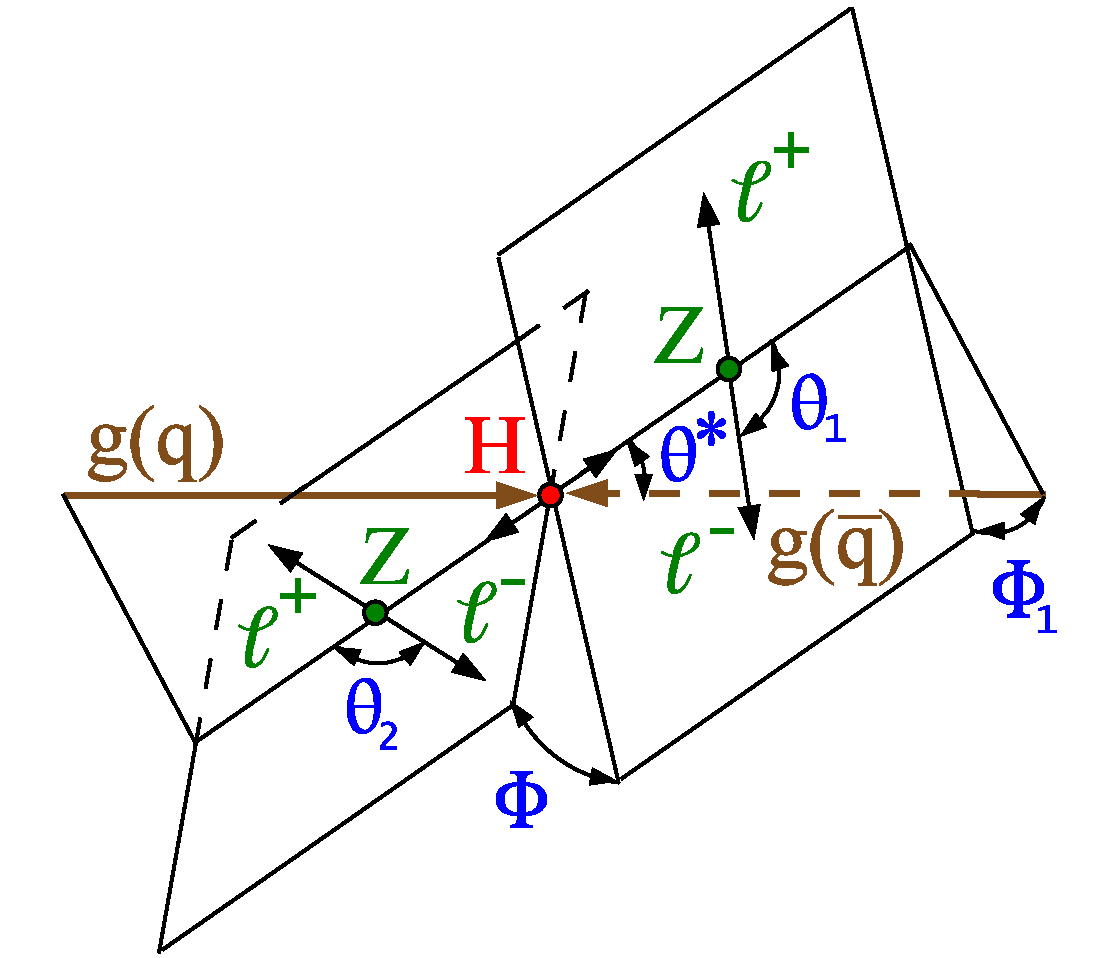
\includegraphics[width=0.57\columnwidth]{Images/H4L/KinematicObservables/angles-h4l.pdf}}
	\caption{Illustration of the $gg/q\bar{q}\to \PH\to ZZ\to 4\ell^\pm$ process. The angular variables reported are considered in the measurements in this analysis. }
	\label{fig:decayHZZ4l}
\end{figure}

The angle $\theta^\star$ is defined as the angle between the beam axis and the direction of the $\PZ_1$ candidate in the event, while $\phi$ and $\phi_1$ are defined as the angles between the three planes containing the \PH boson and the decay products of the $\PZ_1$ and $\PZ_2$ candidates. 
The angles $\theta_1$ and $\theta_2$ are defined as the angles between the $\PZ_1$ and $\PZ_2$ flight directions and the planes containing the di-lepton systems originating from their decay.
In addition, the $\Pp\Pp\to\Hllll$ fiducial cross section is measured in differential bins of the invariant masses of the $\PZ_1$ and $\PZ_2$ candidates.
The set comprising these two observables and the five angles defined above is hereafter referred to as $\vec\Omega^{\HZZfl}\left(\theta^\star,\theta_1,\theta_2,\phi,\phi_1,m_{\PZ_1},m_{\PZ_2}| m_{4\ell}\right)$ and it defines the seven degrees of freedom that completely characterise the $\HZZfl$ process.
The $\vec\Omega^{\HZZfl}$ retains the maximal information present in an event and it can be used to build matrix element discriminants sensitive to the decay of the four lepton final state, as further detailed in Section \ref{sec:discriminants}.

Differential fiducial cross sections are also measured in bins of kinematic observables associated to the jets present in the event, such as: the number of associated jets ($N^{j}$) and the transverse momentum of the leading ($\pt^{j_1}$) and sub-leading ($\pt^{j_2}$) jets.
For events with two or more jets the properties of the di-jet system are assessed by measuring differential cross sections in bins of its invariant mass ($m_{jj}$) and of their differences in pseudorapidity ($\Delta\eta_{jj}$) and azhimutal angle ($\Delta\phi_{jj}$). 
Fiducial cross sections are also measured in bins of smooth functions of the jet rapidity ($\mathcal{T}_{\text{C}}$ and $\mathcal{T}_{\text{B}}$). Thes observables are designed to serve as jet vetoes complementary to $\pt^{j}$ and $N^{j}$ and they are defined as of Ref.~\cite{Gangal:2014qda}:
\begin{linenomath*}
	\begin{equation}
	\label{eqn:tauC}
	\mathcal{T}_{\text{C}} = \max_{j}\left(\frac{\sqrt{E^2_j-p_{z,j}^2}}{2\cosh\left(y_j-Y_\PH\right)}\right),
	\end{equation}
\end{linenomath*}
\begin{linenomath*}
	\begin{equation}
		\label{eqn:tauB}
		\mathcal{T}_{\text{B}} = \max_{j}\left(m^j_{\text{T}}e^{-\mid y_j-Y_\PH\mid}\right),
	\end{equation}
\end{linenomath*}
computed for all the jets in the event and taken from the maximum among them.

The properties of the \PH+jets system are also studied by measuring differential cross sections in bins of the transverse momentum and invariant mass of the four lepton system and the leading jet ($m_{\PH j}$, $\pt^{\PH j}$), or leading and sub-leading jets ($m_{\PH jj}$, $\pt^{\PH jj}$), for events with at least one or two jets, respectively.

%The choice of the bin boundaries for each measurement has been optimised by varying the widths targeting a similar relative uncertainty on the SM expected cross sections in each bin.
%This criterion is found to be equivalent to a definition based on the maximization of the expected discovery significance.

A summary of all the observables considered in this analysis, together with the bin boundaries used for measurements of differential cross sections, is provided in Tab.~\ref{tab:binBoundaries}. The table details also the target of the measurement, specifying wether a given observable is sensitive to the production or the decay of the $\PH\rightarrow 4\ell$ process.
The observables characteristic of the H+j(j) system or the di-jet system can only be defined in events with at least one (or two) jets. In all the other cases, an additional bin containing all the events for which the observable is undefined is introduced in the measurement. This to ensure not only that the integrated cross section corresponds to the SM prediction for the fiducial volume considered in the analysis, but also to account for possible bin-by-bin migrations between generator-level and reconstruction-level events.

\begin{table}[tbp]
	\centering 
	\caption{Variables considered in the analysis and their bin boundaries.}
	\resizebox{\textwidth}{!}{
		\renewcommand{\arraystretch}{1.5}
		\begin{tabular}{lccc}
			Variable & Definition & Bin boundaries & Target \\
			\hline
			$\mH$ &    Invariant mass of the $4\ell$ system       & [105,140] & Inclusive\\
			$\pt^\PH$ & Transverse momentum of the $4\ell$ system  & [0,10,20,30,45,80,120,200,$\infty$) & Production\\
			$|y_\text{H}|$ & Rapidity of the $4\ell$ system  & [0,0.15,0.3,0.6,0.9,1.2,2.5] & Production \\
			$cos \theta^*$ &  Cosine of the decay angle of the leading lepton pair in the $4\ell$ rest frame system  & [0,0.2,0.4,0.6,0.8,1.0] & Decay \\
			$cos \theta_1$, $cos \theta_2$  &  Cosine of the production angle, relative to the $Z$ vector, of the anti-leptons from the two $Z$ bosons & [0,0.2,0.4,0.6,0.8,1.0] & Decay \\
			$\phi$, $\phi_1$ & Azimuthal angles between the decay planes & [0,0,6,1.2,1.8,2.4,3] & Decay \\
			$m_{Z1}$ & Invariant mass of the two leading leptons & [40,65,73,80,85,90,120] & Decay  \\
			$m_{Z2}$ & Invariant mass of the two sub-leading leptons & [12,24,28,32,40,48,65] & Decay \\
			$\pt^{\text{j}_1}$ & Transverse momentum of the leading jet& [0,30,55,95,200,$\infty$) & Production \\
			$\pt^{\text{j}_2}$ & Transverse momentum of the sub-leading jet& [0,30,55,95,200,$\infty$) & Production \\
			$N^{j}$, $N^{j\text{, b-tag}}$&  Number of jets and b-tagged jets& $=$0,$=$1,$=$2,$=$3,$\geq$4 & Event level \\
			$\mathcal{T}_{\text{C}}$, $\mathcal{T}_{\text{B}}$ &  Rapidity weighted jet vetoes & [0,5,10,15,20,25,40,80,$\infty$) & Event level \\
			$m_{jj}$ & Invariant mass of the leading and sub-leading jets system & [120,400,$\infty$) & Production\\
			$\Delta\phi_{jj}$ & Difference in azimuthal angles of the leading and sub-leading jets & $[-\pi,-\pi/2,0,\pi/2,\pi]$ & Production\\
			$\Delta\eta_{jj}$ & Difference in pseudorapidities of the leading and sub-leading jets & [0,0.7,1.6,3.0,10.0] & Production\\
			$\pt^{\PH j}$ & Transverse momentum of the $4\ell$ and leading jet system & [0,60,120,350] & Mixed\\
			$m_{\PH j}$ & Invariant mass of the $4\ell$ and leading jet system & [120,180,220,300,400,600,2000] & Mixed\\
			$\pt^{\PH jj}$ & Transverse momentum of the $4\ell$, leading and sub-leading jets system & [0,60,120,350] & Mixed\\
			$m_{\PH jj}$ & Invariant mass of the $4\ell$, leading and sub-leading jets system & [180,320,450,600,1000,2500] & Mixed\\
		\end{tabular}
	}
	\label{tab:binBoundaries}
\end{table}

A series of double differential cross section measurements is also presented in this analysis with the goal of probing phase space regions of the $\HZZfl$ decay never studied in detail so far in a four-lepton analysis.
%The bins for these measurements are defined with the same approach employed for one dimensional case by adjusting the boundaries targeting a similar relative uncertainty in each bin.
%An example of the bin boundaries adopted for the measurement of the fiducial cross sections in double differential bins of $m_{Z1}$ and $m_{Z2}$ is given in Fig.~\ref{fig:mZ1_mZ2_binning}.
%The boundaries divide the $m_{Z1}$ - $m_{Z2}$ plane in five regions chosen to collect the majority of signal events in two bins, while leaving the most of backgournd event in the other three bins.

%\begin{figure}[tbp]
%	\centering
%	{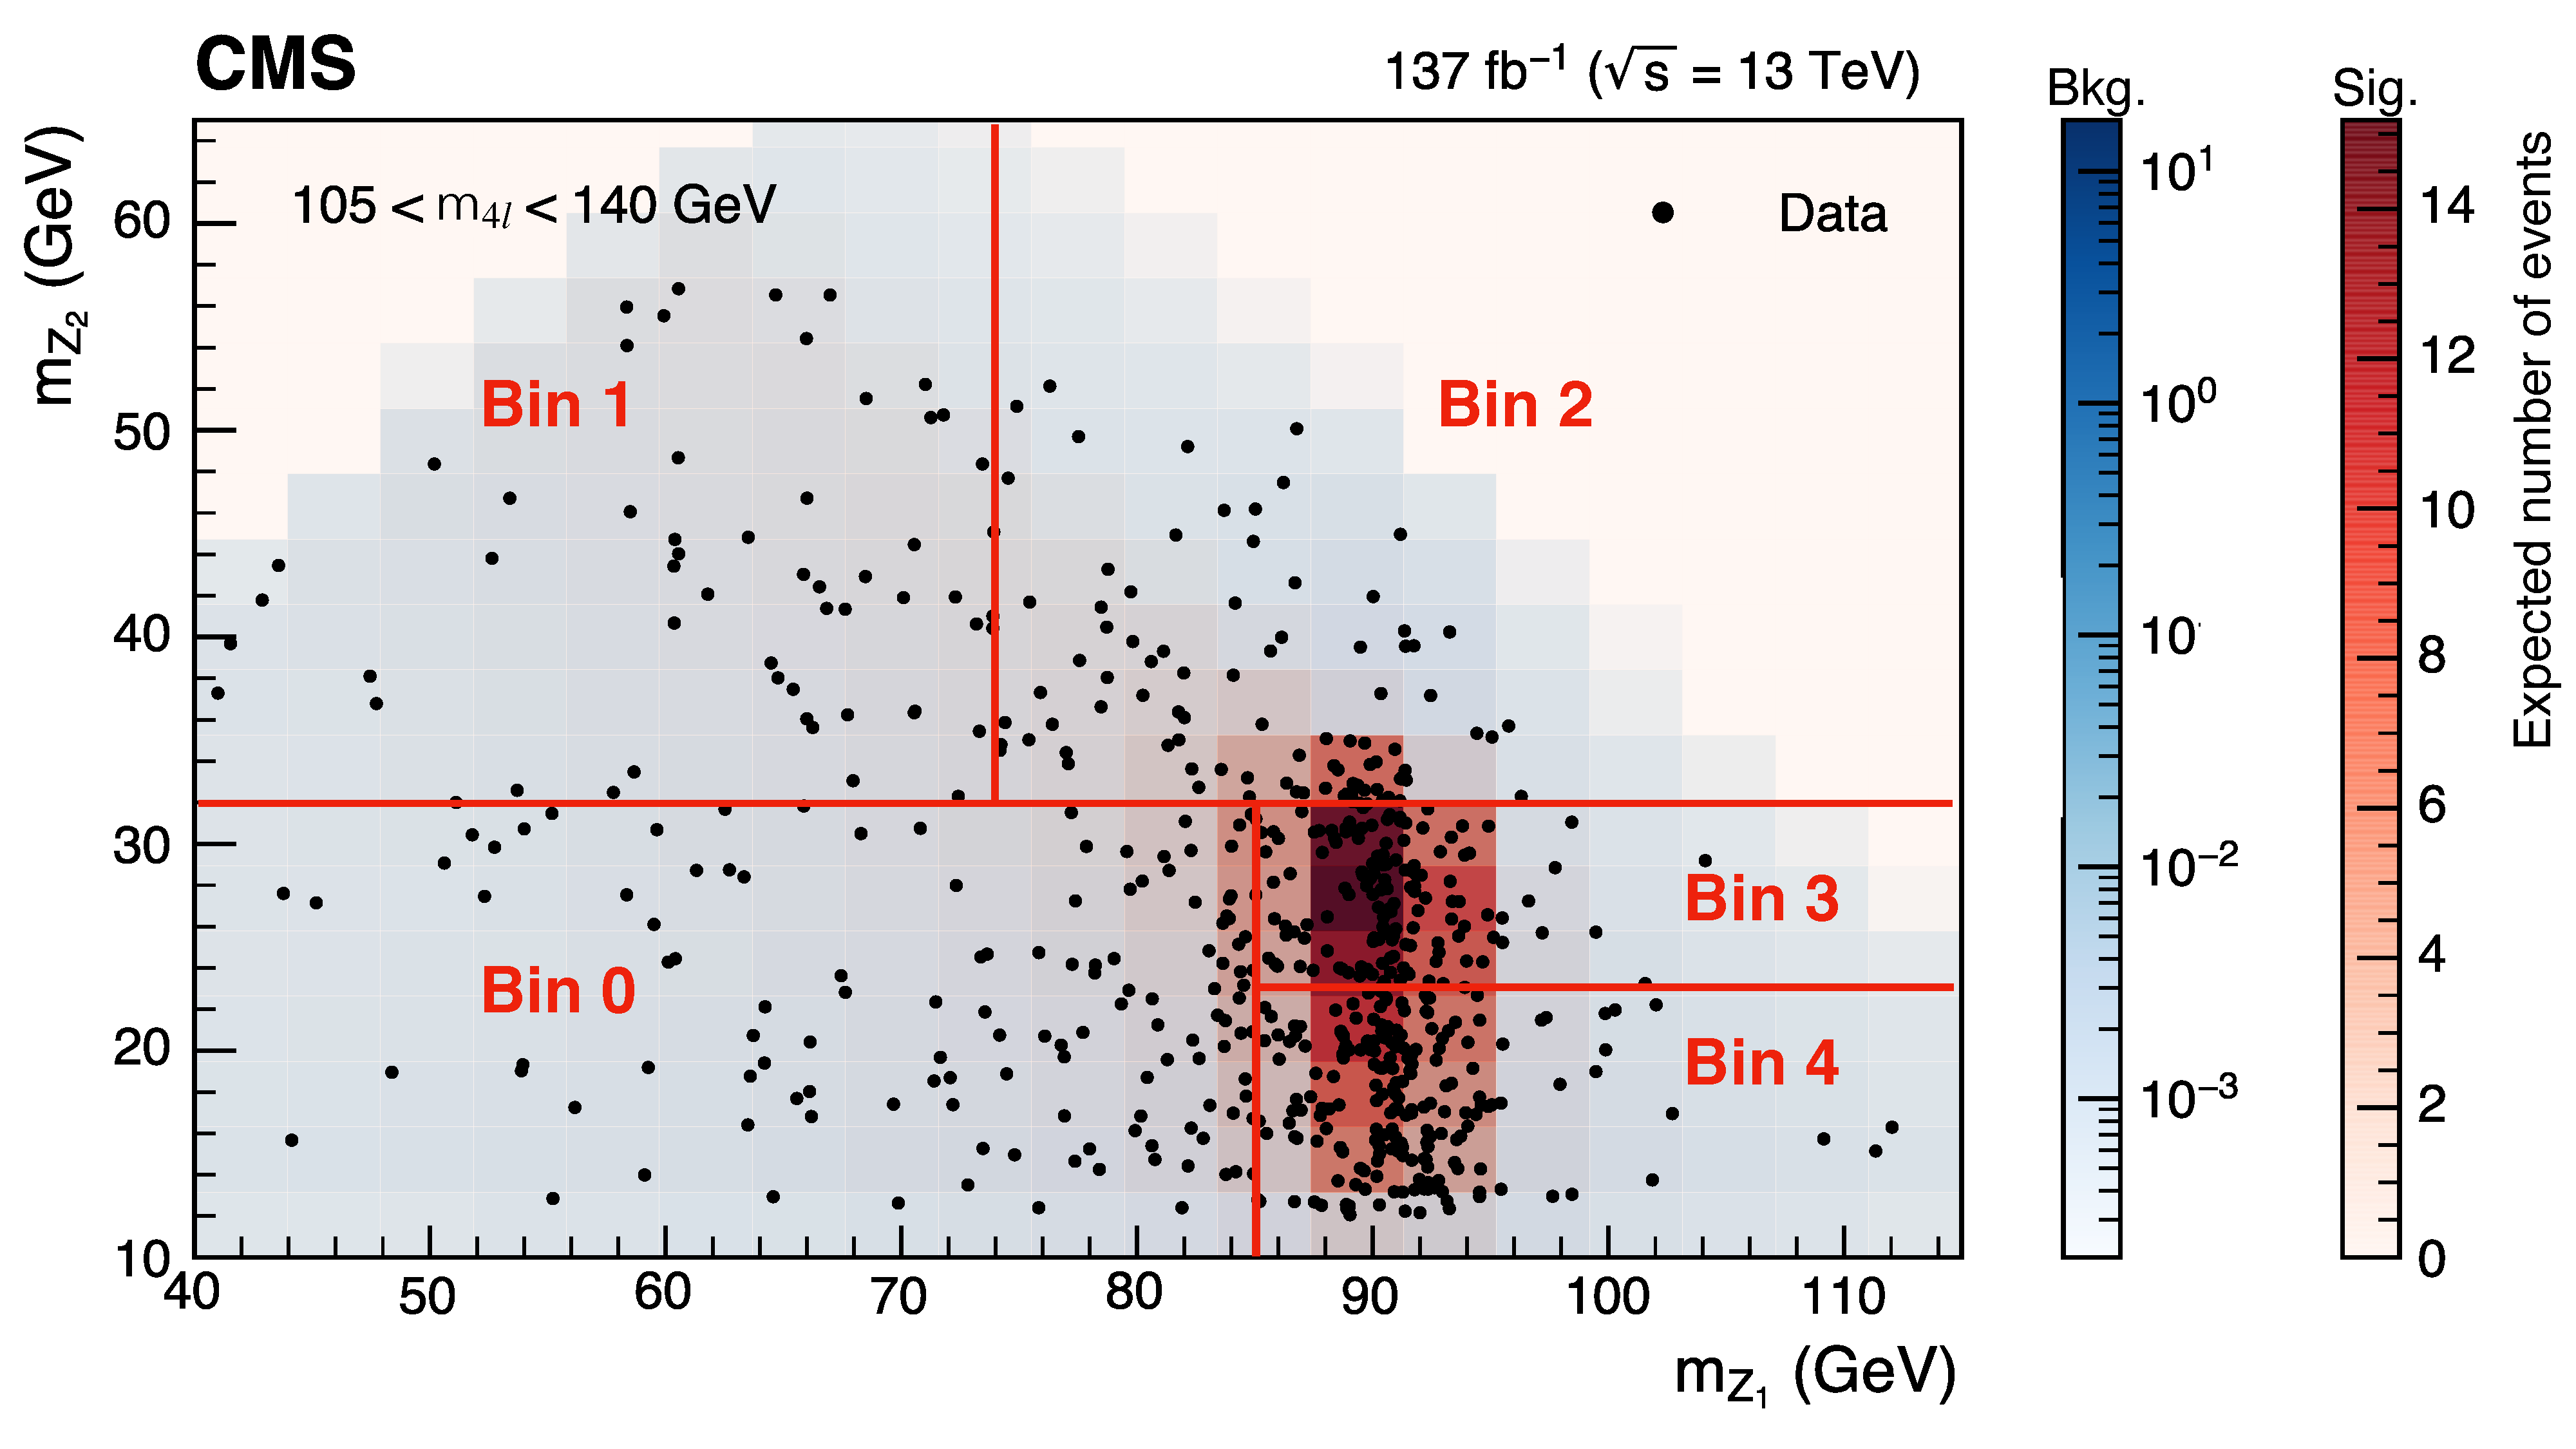
\includegraphics[width=\columnwidth]{Images/H4L/KinematicObservables/mZ1_mZ2_binning}}
%	\caption{Binning for double differential measurement in  $m_{\PZ_{1}}$ - $m_{\PZ_{2}}$.}
%	\label{fig:mZ1_mZ2_binning}
%\end{figure}

The list of the double differential measurements performed in this analysis is reported in Table~\ref{tab:2Dmeasurements},  specifying wether they are sensitive to the production or the decay of the $\PH\rightarrow 4\ell$ process.
The bin boundaries are defined by simultaneous cuts on the two observables that enter the measurement and are detailed for each case separately in Sec.~\ref{sec:results}.

\begin{table}[tbp]
	\centering 
	\caption{Variables considered in the analysis and their bin boundaries.}
	\resizebox{\textwidth}{!}{
		\renewcommand{\arraystretch}{1.5}
		\begin{tabular}{lcc}
			Variable & Definition & Target \\
			\hline
			$\pt^\PH$ vs $|y_\text{H}|$ &  Transverse momentum and rapidity of the 4$\ell$ system & Production\\
			$\pt^\PH$ vs $\mathcal{T}_{\text{C}}$ &  Transverse momentum of the  4$\ell$ system and rapidity-weighted jet veto & Production \\
			$\pt^\PH$ vs $N^{j}$ &  Transverse momentum of the 4$\ell$ system and number of jets in the event  & Production\\
			$m_{\PZ_{1}}$ vs $m_{\PZ_{1}}$ &    Invariant masses of the two $Z$ boson candidates & Decay\\
			$\pt^{j_1}$ vs $\pt^{j_2}$ &  Transverse momenta of the leading and sub-leading jets & Production \\
			$\pt^\PH$ vs $\pt^{\PH j}$ &  Transverse momentum of the 4$\ell$ and 4$\ell$+leading-jet  systems & Production\\
		\end{tabular}
	}
	\label{tab:2Dmeasurements}
\end{table}
%
\subsection{Matrix element discriminants}
\label{sec:discriminants}
The JHUGen and MCFM generators used for the simulation of signal and background events can be used to compute the matrix element probability $\mathcal{P}_a$ for  an event to arise from a physical process $a$, given the value of the reconstructed invariant mass of the four-lepton system $\mllll$, as a function of the set of kinematic observables $\vec\Omega^{\HZZfl}$ defined in Sec.~\ref{sec:observables}.
These probabilities are computed exploiting all the degrees of freedom of the events and therefore retain the maximal information for the description of the underlying physics contained therein.
Hence, the $\mathcal{P}_i(\vec\Omega^{\HZZfl}), i=a,b$ probabilities can be used to construct likelihood-ratio-like matrix element discriminats to discriminate between two physical processes $a$ and $b$, may them be two different production mechanisms of the SM Higgs boson or the test of a BSM hypothesis agains the SM scenario.
This kind of matrix element discriminants has been widely used in the context of the $\HZZfl$ analyses, from the measurement of the $\PH$ boson properties~\cite{CMSHIG19001} up to the constraints on its anomalous couplings~\cite{CMSHIG19009}.
The general structure of these discriminants is an adaptation of the more classic likelihood-ratio, with a slight modification introduced in its definition to make sure that the discriminants are always bounded between 0 and 1.
In general, two different types of kinematic discriminants can be built:
\begin{linenomath}
	\ifthenelse{\boolean{cms@external}}
	{
		\begin{equation}
		\label{eqn:mela}
		\begin{aligned}
		\Dalt &=
		\frac{ \mathcal{P}_{\text{sig}} (\vec\Omega) }
		{\mathcal{P}_{\text{sig}} (\vec\Omega) + \mathcal{P}_{\text{alt}} (\vec\Omega) } \\
		\Dint &=
		\frac{ \mathcal{P}_{\text{int}} (\vec\Omega) }
		{2\cdot\sqrt{\mathcal{P}_{\text{sig}} (\vec\Omega) \cdot \mathcal{P}_{\text{alt}} (\vec\Omega)} },
		\end{aligned}
		\end{equation}
	}
	{
		\begin{equation}
		\label{eqn:mela}
		\begin{aligned}
		\Dalt &=
		\frac{ \mathcal{P}_{\text{sig}} (\vec\Omega) }
		{\mathcal{P}_{\text{sig}} (\vec\Omega) + \mathcal{P}_{\text{alt}} (\vec\Omega) }
		\,\,\,\,\,
		\Dint &=
		\frac{ \mathcal{P}_{\text{int}} (\vec\Omega) }
		{2\cdot\sqrt{\mathcal{P}_{\text{sig}} (\vec\Omega) \cdot \mathcal{P}_{\text{alt}} (\vec\Omega)} },
		\end{aligned}
		\end{equation}
	}
\end{linenomath}

where $\mathcal{P}_{\text{sig}}$ and $\mathcal{P}_{\text{alt}}$ are the SM and BSM probabilities of an event given its kinematic properties in $\vec\Omega$, and $\mathcal{P}_{\text{int}}$ is their interference. 
%These computations rely on the matrix element likelihood apporach implemented in the \textsc{MELA} package~\cite{Gao:2010qx,Bolognesi:2012mm,Anderson:2013afp,Gritsan:2020pib} and exploit the \textsc{jhugen} matrix elements for the signal and the \MCFM matrix elements for the background.

%The full event kinematics is represented by decay observables $\vec\Omega^{\PH\to4\ell}$ that are used to build the set of matrix element discriminant sensitive to the SM \PH boson.
For this analysis a total of six matrix element discriminants, sensitive to different anomalous couplings of the $\PH$ boson, are used to achieve a complete characterisation of the $\PH\to4\ell$ decay.
Tab.~\ref{tab:MEdiscriminants} details the set of kinematic discriminants considered, together with the coupling to which they are sensitive.

\begin{table}[tbp]
	\centering 
	\caption{Matrix element kinematic discriminants considered in the analysis.}
	\renewcommand{\arraystretch}{1.5}
	\begin{tabular}{ ccccc|cc  }
		& \multicolumn{4}{c}{\Dalt}& \multicolumn{2}{c}{\Dint} \\
		\cline{2-7}
		& \multicolumn{6}{c}{Coupling} \\
		& a$_3$ & a$_2$ & $\kappa_1$ & $\kappa_2^{\PZ,\gamma}$ & a$_3$ & a$_2$ \\
		Discriminant & \Dzm & \Dzhp & \DLone & \DLoneZg & \DCP & \Dint \\
	\end{tabular}
	\label{tab:MEdiscriminants}
\end{table}

The $a_i$  and $\kappa_i$ terms correspond to the strengths of vector-boson couplings, following the same notation adopted in Ref.~\cite{CMSHIG19009}.
In particular, the  a$_3$ CP-odd term is expected to be null in the SM and therefore it is sensitive to possible BSM effects that would result in CP violation.
The a$_2$ term correspond to the CP-even contribution to the $\PH\PV\PV$ coupling and it is sensitive to possible BSM contributions from heavy $\PH$ bosons.
The $\kappa_i$ terms are sensitive to possible physics at new energy scale $\Lambda_{1}$ for the VV and the $\PZ \gamma$ couplings respectively.

Differential cross sections are measured in bins of these six matrix element discriminants under the SM hypothesis.
The compatibility of the measurements with the SM predictions is assessed comparing the results with the discriminants built for alternative BSM scenarios, where HVV anomalous couplings of the \PH boson are introduced.

For these observables, as well as for all the ones sensitive to the decay side of the process under study, differential cross sections are measured both for the inclusive $4\ell$ final state and for the $4\Pgm+4\Pe$ and $2\Pe2\Pgm$ final states separately.
This choice is driven by the fact that the same-leptons final states have different physics than the $2\Pe2\Pgm$  final state beacuse of the destructive interference between the two alternative ways of constructing the $\HZZfl$ diagrams in the same-helicity cases.
Presenting the results with this distinction between final states enhances the model-independence of the measurements and widens their possible application, without the need of \textit{ad hoc} assumptions, in their re-interpretations.
%Besides providing the best test statistics to discriminate between two hypotheses, represented by the corresponding probabilities $\mathcal{P}$, the MELA approach is completely reproducible as it relies on phenomenological calculations of the matrix element for the process under study, therefore enhancing the feasibility of \textit{a posteriori} re-interpretations of the results.

\section{Background estimation}
\label{sec:bkgd}

\subsection{Irreducible backgrounds}
\label{sec:irrbkgd}
The irreducible $\PZ\PZ$ background contribution originated from $\Pq\Paq$ annihilation or gluon fusion is estimated from simulation. 
The former is simulated at NLO pQCD with \POWHEG~2.0 and reweighted to NNLO using a K factor computed as a function of $m_{\PZ\PZ}$ exploiting the NNLO computation of the $\qqZZ$ fully differential cross section~\cite{Grazzini2015407}.
The effect of this K factor ranges between 0 and 20\% and is 10\% at $m_{\PZ\PZ}=125\GeV$.
Additional NLO electroweak corrections are extracted from Ref.~\cite{Bierweiler:2013dja} and are applied in the $m_{\PZ \PZ}>2m_{\PZ}$ region depending on the initial state quark flavor and kinematics.

The soft collinear approximation is proven to describe accurately the cross section and the interference term for the gluon fusion $\PZ\PZ$ contribution at NNLO\@~\cite{Bonvini:1304.3053} in pQCD.
In addition, further calculations demonstrate that the K factors are very similar at NLO for signal and background~\cite{Melnikov:2015laa} and at NNLO for signal and interference terms~\cite{Li:2015jva}.
Hence, the same K factor is used for signal and background~\cite{Passarino:1312.2397v1}.
The \textsc{hnnlo}~v2 program~\cite{Catani:2007vq,Grazzini:2008tf,Grazzini:2013mca} is used to obtain the signal NNLO K factor as a function of $m_{\PZ\PZ}$ from the ratio of the NNLO and LO $\Pg\Pg\to\PH\to2\ell2\ell^\prime$ cross sections for the $\PH$ boson decay width of 4.07\MeV. 
The NNLO/LO K factor for {\ggZZ} varies from $\approx$2.0 to 2.6 and is 2.27 at $m_{\PZ\PZ}=125\GeV$, with a 10\% systematic uncertainty for the background process.

%The background processes arising from triboson production $\PZ\PZ\PZ$, $\PW\PZ\PZ$, and $\PW\PW\PZ$, as well as $\ttZ$, $\ttWW$, and $\ttZZ$ are also considered.
%These processes are all estimated from simulation and are referred to as the EW backgrounds in the analysis.

The contribution of these irreducible background processes is included in the form of binned templates in the likelihood function used to extract the differential cross section measurements and it is derived independently in the three final states considered ($4\Pgm$, $4\Pe$, and $2\Pe 2\Pgm$).
The normalisation of these templates is extracted directly from MC, exploiting the most accurate theoretical calculations available to date.
In order to estimate the impact of the theoretical uncertainty on these background normalisations on the inclusive $\Hllll$ fiducial cross section, an additional measurement is performed leaving the normalisation of the irreducible $\PZ\PZ$ processes freely floating in the fit and constraining it through a fit of data in the sidebands of the $\PH$ peak.

\subsection{Reducible background}
\label{sec:redbkgd}
The reducible background contribution to the \PH boson signal in the $4\ell$ channel mainly comes from the $\PZ\text{+jets}$,  $\ttbar\text{+jets}$,
$\PZ\gamma\text{+jets}$, $\PW\PW\text{+jets}$, and $\PW\PZ\text{+jets}$ production, hereafter collectively referred to as $\PZ\text{+jets}$ process.

The contribution from the reducible background is estimated exploiting the same data driven technique emploied in Ref.~\cite{CMSHIG19001} based on lepton misidentification rates and control regions comprising a $\PZ$ candidate and one ($\PZ+\ell$) or two ($\PZ+\ell\ell$) \textit{loose} leptons.

The shapes of the $\PZ\text{+jets}$ reducible background are derived for the three final states ($4\Pgm$, $4\Pe$, and $2\Pe 2\Pgm$) separately and are included as binned templates in the likelihood function used for the statistical analysis.

\section{Signal modelling}
\label{sec:signal}

The parametrization of the $\PH$ resonance as a function of $\mH$ is extracted from a simultaneous fit of signal samples generated at various mass points, following the same approach detailed in Ref.~\cite{CMSHIG19001}.
The normalization of the double-sided Crystal Ball is proportional to $\sigma_{\mathrm{fid}}$, the fiducial cross section and parameter of interest of the analysis.

The shape of the \PH resonant signal, hereafter referred to as $\mathcal{P}(\mllll)$, is described by a double-sided Crystal Ball function~\cite{Oreglia:1980cs} around $\mH \approx 125\GeV$.
The parametrisation of the signal model as a function of $\mH$ is obtained independently for each production mechanism by performing a simultaneous fit of several mass points  in the 105 to 160\GeV mass range.
The non-resonant contribution to the signal in the case of $\WH$, $\ZH$ and $\ttH$ production modes is modelled with the inclusion of a  Landau function in the total probability density function . 
Each parameter of the double-sided Crystal Ball function has a linear dependence on $\mH$, for a total of 12 free parameters.
% Fig.~\ref{fig:signal_fit} depicts the results of the fit for the $\ggH$ production mode in the $4\Pe$ and $4\mu$ final states. 

% \begin{figure}[!htb]
% 	\centering
% 	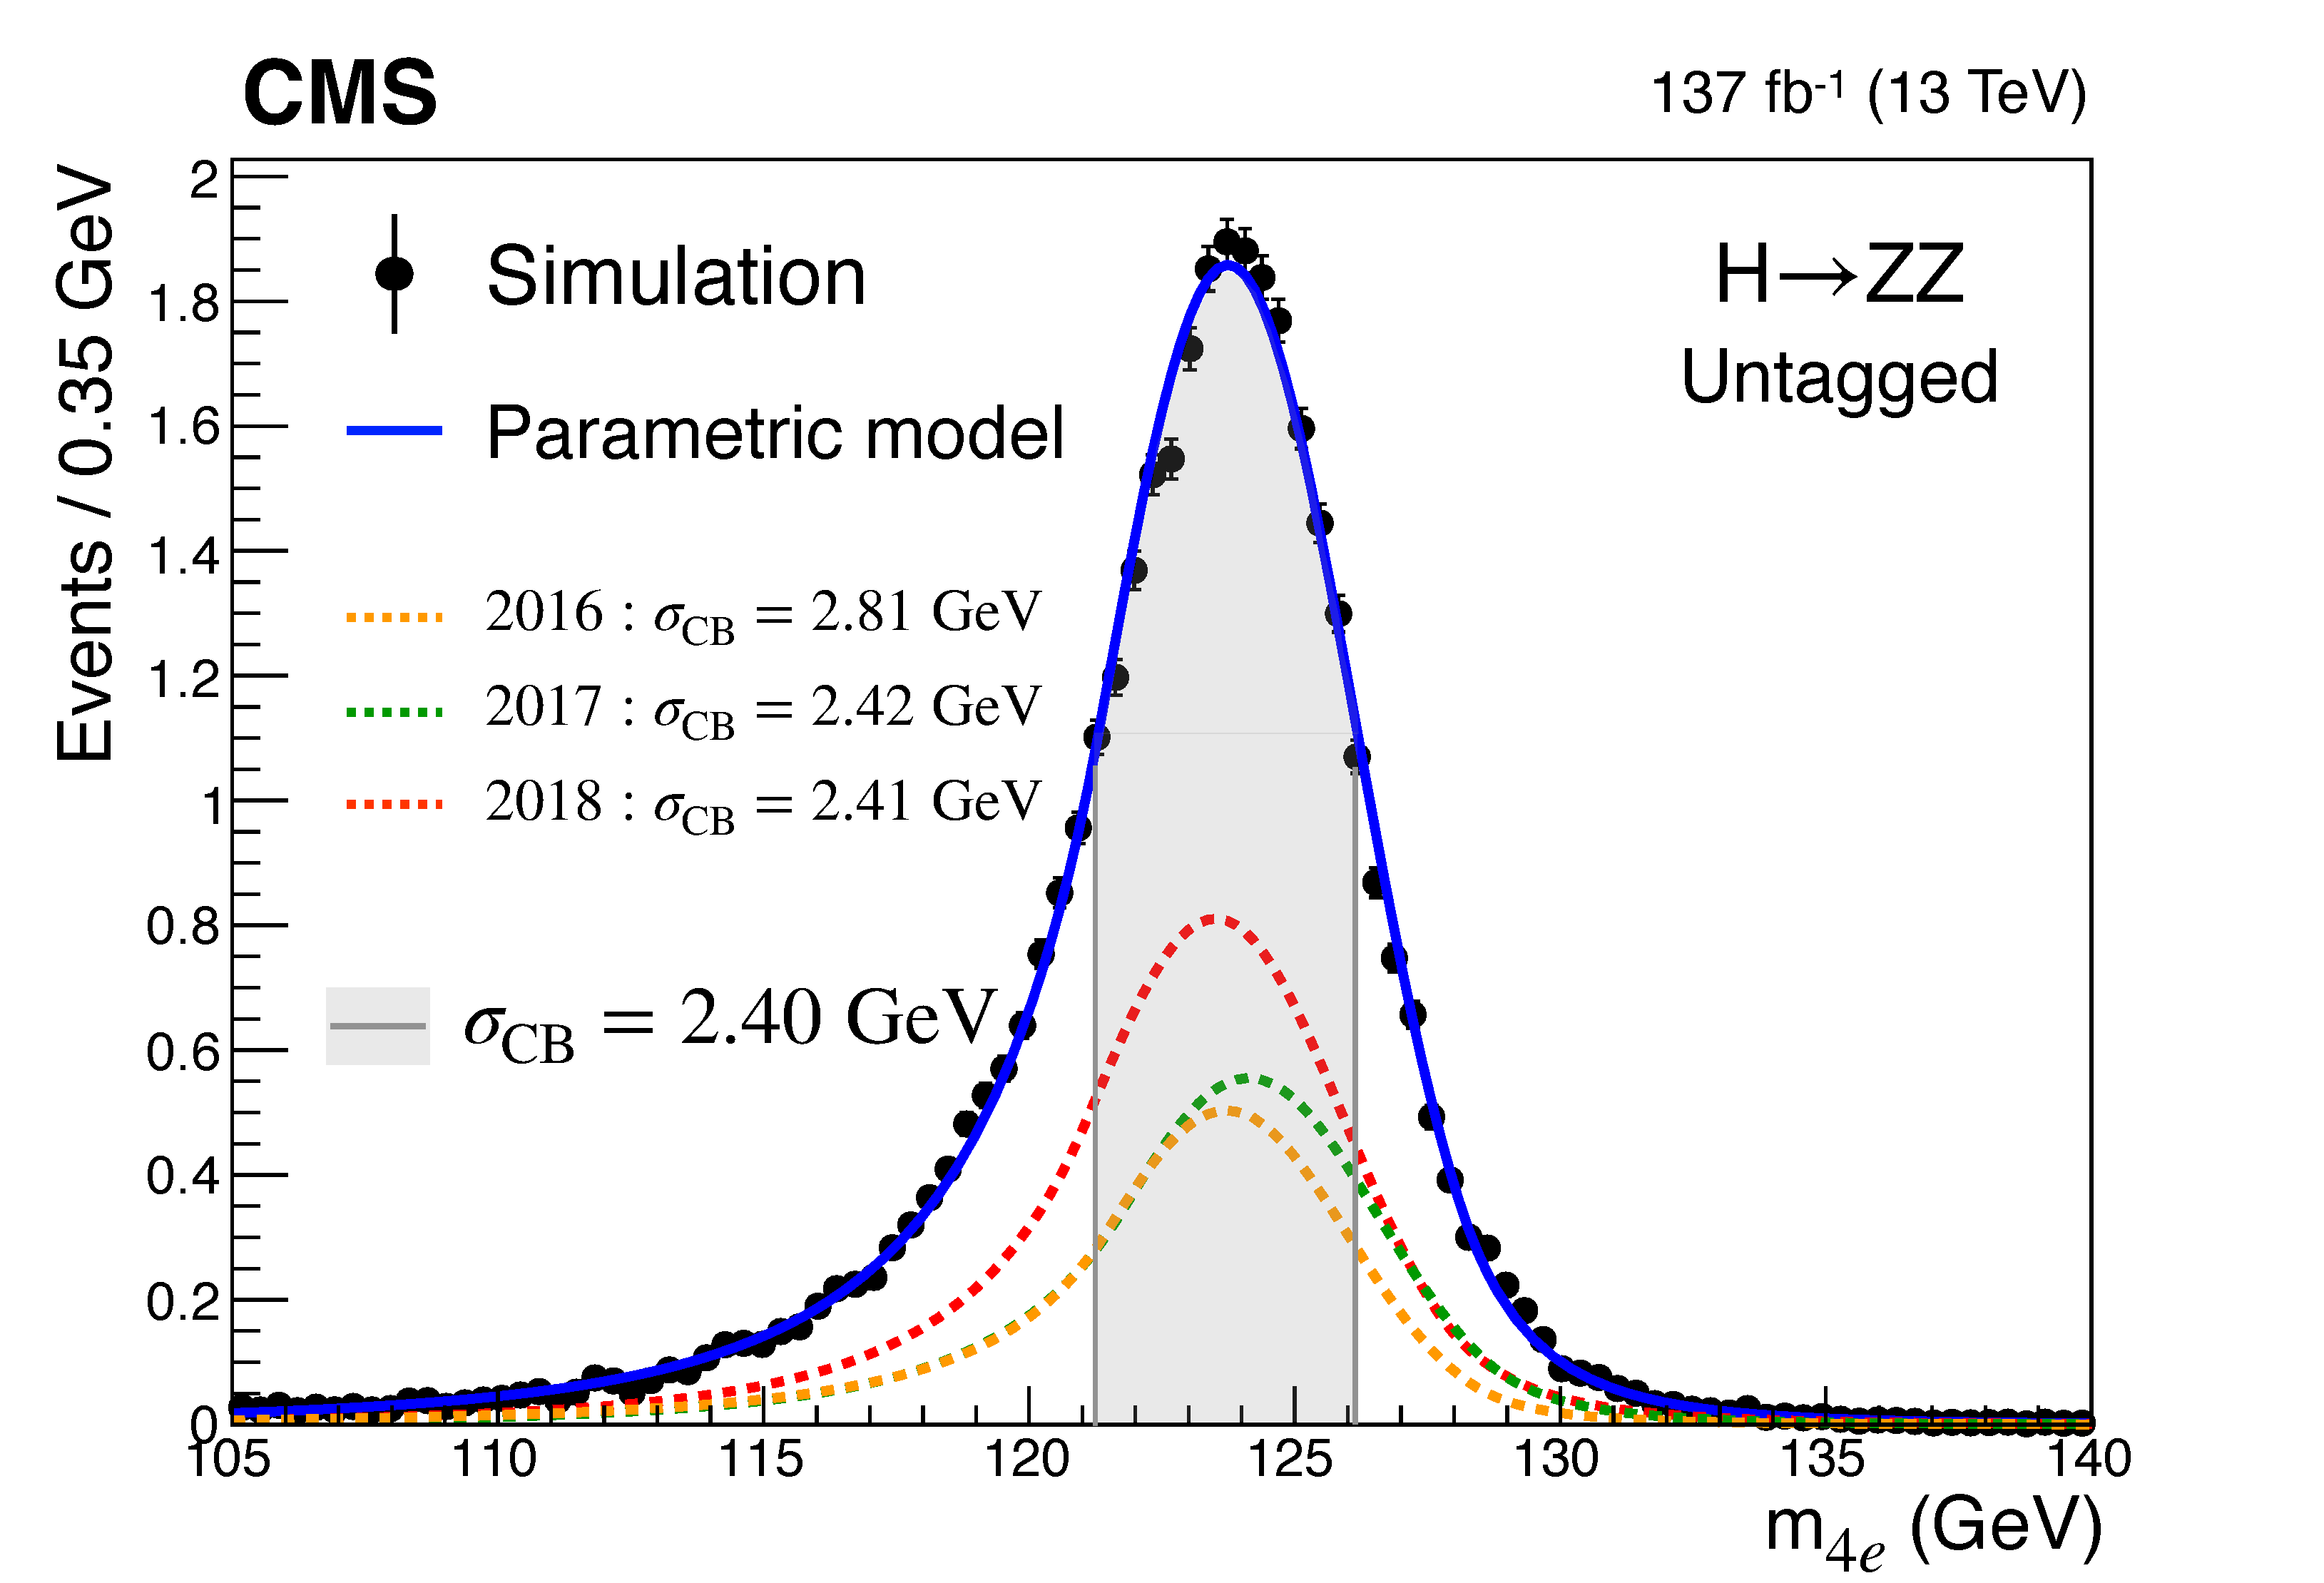
\includegraphics[width=0.49\textwidth]{Images/H4L/Signal/HZZ4e_lineshape.pdf}
% 	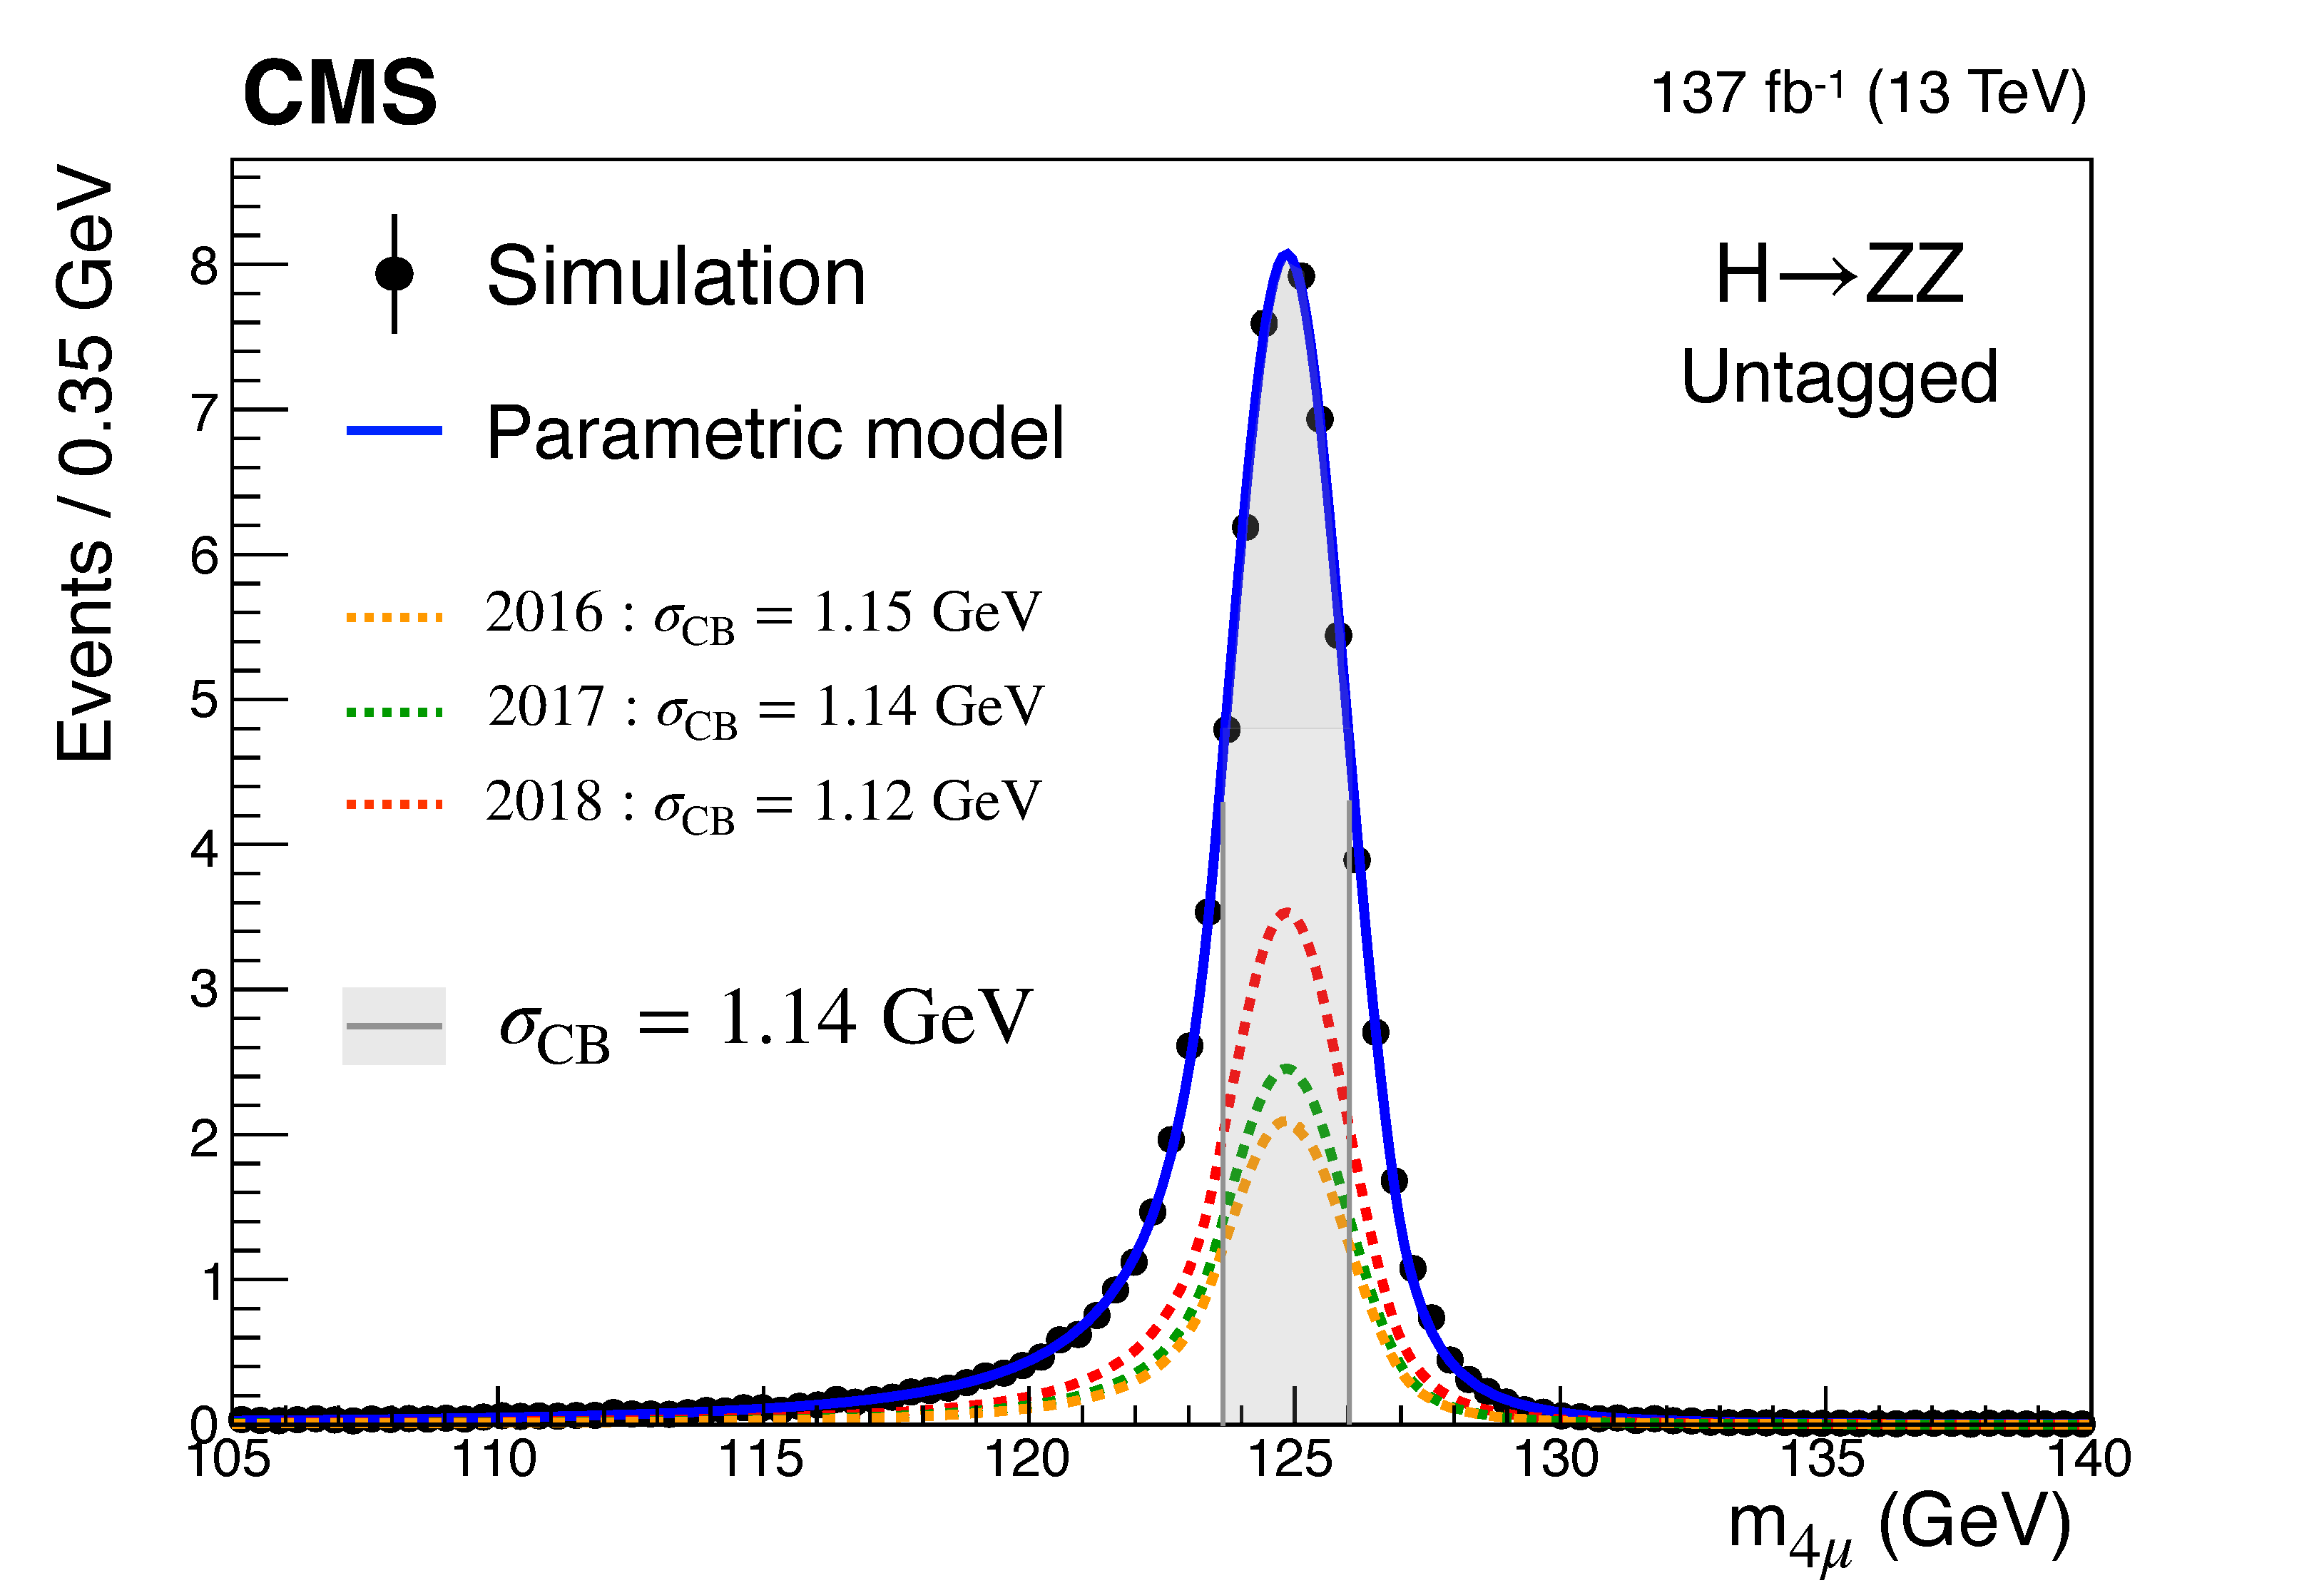
\includegraphics[width=0.49\textwidth]{Images/H4L/Signal/HZZ4mu_lineshape.pdf}
% 	\caption{
% % 		\textcolor{red}{\textbf{EDIT, TAKEN FROM 19001}}
% 		The shape of the parametric signal model for each year of simulated data, and for the sum of all years together.
% 		The black points represent weighted simulation events of the $\ggH$ production mechanism for $\mH=125\GeV$ and the blue line the corresponding model.
% 		Also shown is the $\sigma_{\text{CB}}$ value (half the width of the narrowest interval containing 68\% of the invariant mass distribution) in the gray shaded area.
% 		The contribution of the signal model from each year of data-taking is illustrated with the dotted lines.
% 		The models are shown for the $4\Pe$ (\cmsLeft) and $4\Pgm$ (\cmsRight) final states in the untagged event category.
% 		\label{fig:signal_fit}}
% \end{figure}

\section{Measurement methodology}
\label{sec:measurement}

The $\Pp\Pp\to\Hllll$ cross section is measured within a fiducial volume defined as detailed in Section \ref{sec:fiducialvolume}.
%The integrated fiducial cross section is measured as well as differential cross sections as a function of several kinematic observables sensitive to both the production and the decay sides of the $\Pp\Pp\to\Hllll$ process. 
%In order to enhance the sensitivity to specific phase space regions and probe in more detail the SM predictions, double differential cross section measurements are also performed.
%The SM predictions for the \PH boson decay into four lepton are tested against different BSM scenarios by measuring cross sections in differential bins of the matrix element kinematic discriminants introduced in Section~\ref{sec:discriminants}.

The measurements are extracted by means of a maximum likelihood fit of the signal and background distributions to the observed $4\ell$
mass distribution, $N_{\mathrm{obs}}(\mllll)$, defined in each final state $f$ and in each bin $i$ of a given observable as:

\begin{linenomath}
	\ifthenelse{\boolean{cms@external}}
	{
		\begin{equation}
		\label{eqn:m4l}
		\begin{aligned}
		N_{\mathrm{exp}}^{f,i}(m_{4\ell}) &= N_{\mathrm{fid}}^{f,i}(m_{4\ell})+N_{\mathrm{nonfid}}^{f,i}(m_{4\ell})+N_{\mathrm{nonres}}^{f,i}(m_{4\ell})\\
		&+N_{\text{bkg}}^{f,i}(m_{4\ell}) \\
		&=\sum_j\epsilon_{i,j}^{f}  \left(1+f_{\mathrm{nonfid}}^{f,i} \right)\sigma_{\mathrm{fid}}^{f,j}  \mathcal{L}\mathcal{P}_{\mathrm{res}}(m_{4\ell}) \\
		&\,\,\,+ N_{\mathrm{nonres}}^{f,i}\mathcal{P}_{\mathrm{nonres}}(m_{4\ell})+N_{\text{bkg}}^{f,i}\mathcal{P}_{\text{bkg}}(m_{4\ell}).
		\end{aligned}
		\end{equation}
	}
	{
		\begin{equation}
		\label{eqn:m4l}
		\begin{aligned}
		N_{\mathrm{exp}}^{f,i}(m_{4\ell}) &= N_{\mathrm{fid}}^{f,i}(m_{4\ell})+N_{\mathrm{nonfid}}^{f,i}(m_{4\ell})+N_{\mathrm{nonres}}^{f,i}(m_{4\ell})+N_{\text{bkg}}^{f,i}(m_{4\ell}) \\
		&=\sum_j\epsilon_{i,j}^{f}  \left(1+f_{\mathrm{nonfid}}^{f,i} \right)\sigma_{\mathrm{fid}}^{f,j}  \mathcal{L}\mathcal{P}_{\mathrm{res}}(m_{4\ell}) \\
		&\,\,\,+ N_{\mathrm{nonres}}^{f,i}\mathcal{P}_{\mathrm{nonres}}(m_{4\ell})+N_{\text{bkg}}^{f,i}\mathcal{P}_{\text{bkg}}(m_{4\ell}).
		\end{aligned}
		\end{equation}
	}
\end{linenomath}

The resonant signal contribution is parametrized with a double-sided Crystal Ball function, $\mathcal{P}_{\mathrm{res}}(m_{4\ell})$, with a normalization coefficient proportional to the fiducial cross section, $\sigma_{\mathrm{fid}}$.
The results of the fit are extracted as signal strength modifiers by measuring the ratio of $\sigma_{\mathrm{fid}}$  observed in a given fiducial bin to the corresponding SM expectation.
A Landau distribution is introduced to model empirically the shape of the non-resonant signal contribution, $\mathcal{P}_{\mathrm{nonres}}(m_{4\ell})$, for the $\WH$, $\ZH$, and $\ttH$ processes where one of the leptons from the \PH boson decay is either not selected or falls out of the acceptance.
The shape parameters of the Landau distribution are constrained in the fit to be within a range determined from simulation.
These non-resonant events form what is referred to in the analysis as ``combinatorial signal'' and are treated as a background in the measurement.

{\tolerance=800 Detector effects unavoidably introduce differences between the observables used for the fiducial phase space definition and the corresponding quantities at the reconstruction level. 
An additional contribution ($f_{\mathrm{nonfid}}$) is introduced to take into account the presence of events not originating from the fiducial volume but selected for the analysis and it is treated as background in the measurements.
This contribution is referred to as the ``non-fiducial signal'' and it is estimated from simulation for each of the signal models studied.
Dedicated studies on simulation have shown the shape of these events is identical to the shape of the resonant fiducial signal. To minimise the model dependence of the measurement, the value of $f_{\mathrm{nonfid}}$ is fixed to be a fraction of the fiducial signal component.
The values of this fraction are reported in Tab.~\ref{tab:summarySM} and have been found to range between 5\% for the $\ggH$ production mechanism up to 18\% for the $\ttH$ mode.\par}

The quantity $\epsilon_{i,j}^{f}$ represents the detector response matrix that is used to unfold the number of expected events in bin \textit{i} at the reconstruction level to the number of expected events in bin \textit{j} of a given observable at the fiducial level.
Simulated signal samples are used to determine the response matrix, which is also corrected for residual differences between data and simulation.
The measurement of the integrated fiducial cross section is performed within a single bin ($105<\mllll<160\GeV$) and therefore the response matrices become single numbers, listed in Table~\ref{tab:summarySM} for different SM production mechanism.

The table shows also the acceptance $\mathcal{A}_{\mathrm{fid}}$, defined as the fraction of signal events that fall within the fiducial phase space.
%The fraction of signal events within the acceptance of the fiducial phase space, $\mathcal{A}_{\mathrm{fid}}$, and the reconstruction efficiency, $\epsilon$, for the different production mechanisms of the \PH boson are listed in Tab.~\ref{tab:summarySM}. 
%The table also shows the fraction of resonant signal events that do not originate from the fiducial phase space, $f_{\mathrm{nonfid}}$.
%All these quantities, along with the $(1+f_{\mathrm{nonfid}})\epsilon$ factor, are further described in Section~\ref{sec:measurement}.
%It is worth noting the relatively weak dependence of the $(1+f_{\mathrm{nonfid}})\epsilon$ factor on the \PH boson production mechanism resulting from the definition of the fiducial phase space volume and therefore ensuring the model independence of the measurements.

\begin{table*}[!h!tb]
	\centering
	\topcaption{
% 		\textcolor{red}{\textbf{EDIT CAPTIONS, NUMBERS ALREADY UP TO DATE}}
		Summary of the fraction of signal events for different SM signal production modes within the fiducial phase space (acceptance $\mathcal{A}_{\mathrm{fid}}$),
		reconstruction efficiency ($\epsilon$) for signal events in the fiducial phase space,
		and ratio of the number of reconstructed events outside the fiducial phase space to that of the reconstructed events in the fiducial phase space ($f_{\mathrm{nonfid}}$).
		For all production modes the values given are for $\mH = 125\GeV$.
		Also shown in the last column is the factor $(1+f_{\mathrm{nonfid}})\epsilon$ which regulates the signal yield for a given fiducial cross section.
		The uncertainties listed are statistical only. The theoretical uncertainty in $\mathcal{A}_{\mathrm{fid}}$ for the SM is less than 1\%.
		\label{tab:summarySM}
	}
	\begin{tabular}{lcccc}
		Signal process & $\mathcal{A}_{\mathrm{fid}}$ & $\epsilon$ & $f_{\mathrm{nonfid}}$  & $(1+f_{\mathrm{nonfid}})\epsilon$ \\
		\hline
		$\ggH$ (\POWHEG) & 0.408 $\pm$ 0.001 & 0.619 $\pm$ 0.001 & 0.053 $\pm$ 0.001 & 0.652 $\pm$ 0.001 \\
		$\VBF$ & 0.448 $\pm$ 0.001 & 0.632 $\pm$ 0.002 & 0.043 $\pm$ 0.001 & 0.659 $\pm$ 0.002 \\
		$\WH$ & 0.332 $\pm$ 0.001 & 0.616 $\pm$ 0.002 & 0.077 $\pm$ 0.001 & 0.664 $\pm$ 0.002 \\
		$\ZH$  & 0.344 $\pm$ 0.002 & 0.626 $\pm$ 0.003 & 0.083 $\pm$ 0.002 & 0.678 $\pm$ 0.003 \\
		$\ttH$ & 0.320 $\pm$ 0.002 & 0.614 $\pm$ 0.003 & 0.179 $\pm$ 0.003 & 0.725 $\pm$ 0.005 \\
	\end{tabular}
\end{table*}

The systematic uncertainties described in Section~\ref{sec:systematics} are included in the form of nuisance parameters (NPs) and the fiducial cross section measurements are obtained using an asymptotic approach~\cite{LHC-HCG} with a test statistic based on the profile likelihood ratio~\cite{Cowan_2011}.
The maximum likelihood fit is performed simultaneously in all final states and in all bins of the observable under study, assuming a \PH boson mass $\mH=125.38\GeV$.
The branching fractions of the \PH boson to different final states ($4\Pe,4\Pgm,2\Pe2\Pgm$) are left floating in the fit in order to increase the model independence of the measurements, following the same strategy of Ref.~\cite{CMSHIG19001}.
A likelihood-based unfolding procedure is performed to resolve detector effects from the observed distributions to the fiducial phase space. 
This approach is the same as in
Refs.~\cite{Khachatryan:2015yvw}, \cite{CMSHggFiducial8TeV}, and \cite{CMSHIG19001} and it has the advantage of performing simultaneously the unfolding of the detector effects and the likelihood fit to extract the fiducial cross section.
The analysis strategy of Ref.~\cite{CMSHIG19001} is extended here by measuring also double differential cross sections and by measuring the fiducial cross sections in $4\Pgm+4\Pe$ and $2\Pe 2\Pgm$ final states separately when observables targeting the $\Hllll$ decay are considered.
When these measurements are performed, the branching fractions of the \PH boson decay are fixed to the SM expectation.

\section{Systematic uncertainties}
\label{sec:systematics}
The integrated luminosities of the 2016, 2017, and 2018 data-taking periods are individually known with uncertainties in the 1.2--2.5\% range~\cite{CMS-PAS-LUM-17-001,CMS-PAS-LUM-17-004,CMS-PAS-LUM-18-002}, while the total Run~2 (2016--2018) integrated luminosity has an uncertainty of 1.6\%, the improvement in precision reflecting the (uncorrelated) time evolution of some systematic effects. 

Experimental systematic uncertainties due to the trigger and the lepton reconstruction and selection efficiencies are estimated from data for the different final states. 
This uncertainties range from 0.8 to 1.9\% in the 4\Pgm channel and from 6.5 to 11\% in the 4\Pe channel.
Compared to Ref.~\cite{CMSHIG19001} a reduction of about 5\% in the 4\Pe uncertainties has been achieved thanks to a dedicated method introduced in the analysis.
The large difference still present between the two final states reflects the usage of a low mass di-muon resonance for the estimation of the 4\Pgm uncertainties in the low $\pt^{\Pgm}$ regions, whereas only the \PZ boson resonance can be exploited in the 4\Pe channel, yielding to larger uncertainties in the low $\pt^{\Pe}$ region.


{\tolerance=800 The systematic uncertainties on the lepton momentum scale and resolution are estimated from dedicated studies on the $\Zll$ mass distribution in data and simulation.
The scale uncertainty is found to be 0.04\% in the 4\Pgm channel and 0.3\% in the 4\Pe channel, while the resolution uncertainty is 20\% for both channels.
The effect of these uncertainties in introduced in the analysis by floating the corresponding parameters of the double-sided Crystal Ball function used to model the resonant signal as described in Sec.~\ref{sec:signal}.\par} 

Systematic uncertainties on the jet energy scale and smearing are considered when dealing with measurements involving jet-related observables, as they can introduce migrations around the different bin boundaries.
These uncertainties are considered to act on the normalisation of the processes and are modelled with a set of 22 NPs following the central CMS recommendations, taking into account partial correlations among the different sources of uncertainty that impact on the jet energy scale and smearing.
%They can also alter the shape of the discriminants, but the effect on the shape is negligible.

%A systematic uncertainty on the {\PQqb}-tagging efficiency is introduced in the analysis for the measurment of the differential cross section as a function of the number of {\PQqb}-tagged jets.

Experimental systematic uncertainties on the reducible background estimation, described in Section~\ref{sec:redbkgd}, are also considered.
These originate from the background composition and misidentification rate uncertainties vary between 30 and 45\% depending on the final state.
However, the impact of this uncertainty on the measurements is found to be negligible.

Theoretical uncertainties on the renormalization and factorization scales, and the choice of the PDF set affect both the signal and the background rates.
The QCD uncertainty from the renormalization and factorization scales is determined by varying these scales between 0.5 and 2 times their nominal value, while keeping their ratio between 0.5 and 2.
The uncertainty due to the PDF set is determined following the PDF4LHC recommendations by taking the root mean square of the variation of the results when using different replicas of the default NNPDF set~\cite{Botje:2011sn,Alekhin:2011sk}.
An additional 10\% uncertainty in the K factor used for the $\ggZZ$ prediction is applied as described in Section~\ref{sec:irrbkgd}.
A systematic uncertainty of 2\%~\cite{deFlorian:2016spz} in the branching fraction of $\Hllll$ only affects the signal yield.

\section{Results}
\label{sec:results}

\subsection{Inclusive cross section}
The integrated fiducial cross section for the $\HZZfl$ process is measured to be
$$\obsXSECFid$$ at $\mH = 125.38\GeV$
and it is found to be in good agreement with the SM expectation of $\sigma_{{\mathrm{fid}}}^{\mathrm{SM}}=\expXSECFid$, as shown by the corresponding log-likelihood scan in Fig.~\ref{fig:fiducial_LLScan}.
The inclusive fiducial cross section measured in the three final states considered in this analysis ($4\Pgm,\,4\Pe,\,$ and $2\Pe 2\Pgm$)  is shown in the left panel of Fig.~\ref{fig:fiducial_inclusive}, while the right panel depicts the evolution of the $\HZZfl$ fiducial cross section as a function of the center of mass energy.
The results are compared with the cross sections predicted by the POWHEG and NNLOPS generators for the \PH boson production and parton showering, while the decay is always modelled by the JHUGen generator.
In addition to what presented in Ref.~\cite{CMSHIG19001}, the results are also compared with the predictions from the MADGRAPH5\_aMC@NLO generator.
A summary of the measurement is presented in Table~\ref{tab:fiducial_inclusive}, together with a breakdown of the uncertainties into its statistical and systematic components and the results for each individual data taking period analysed.

%%%%%%%%%%%%%%%%%%%%%% Inclusive Fiducial XSEC %%%%%%%%%%%%%%%%%%%%%%

\begin{figure}[!htb]
	\centering
	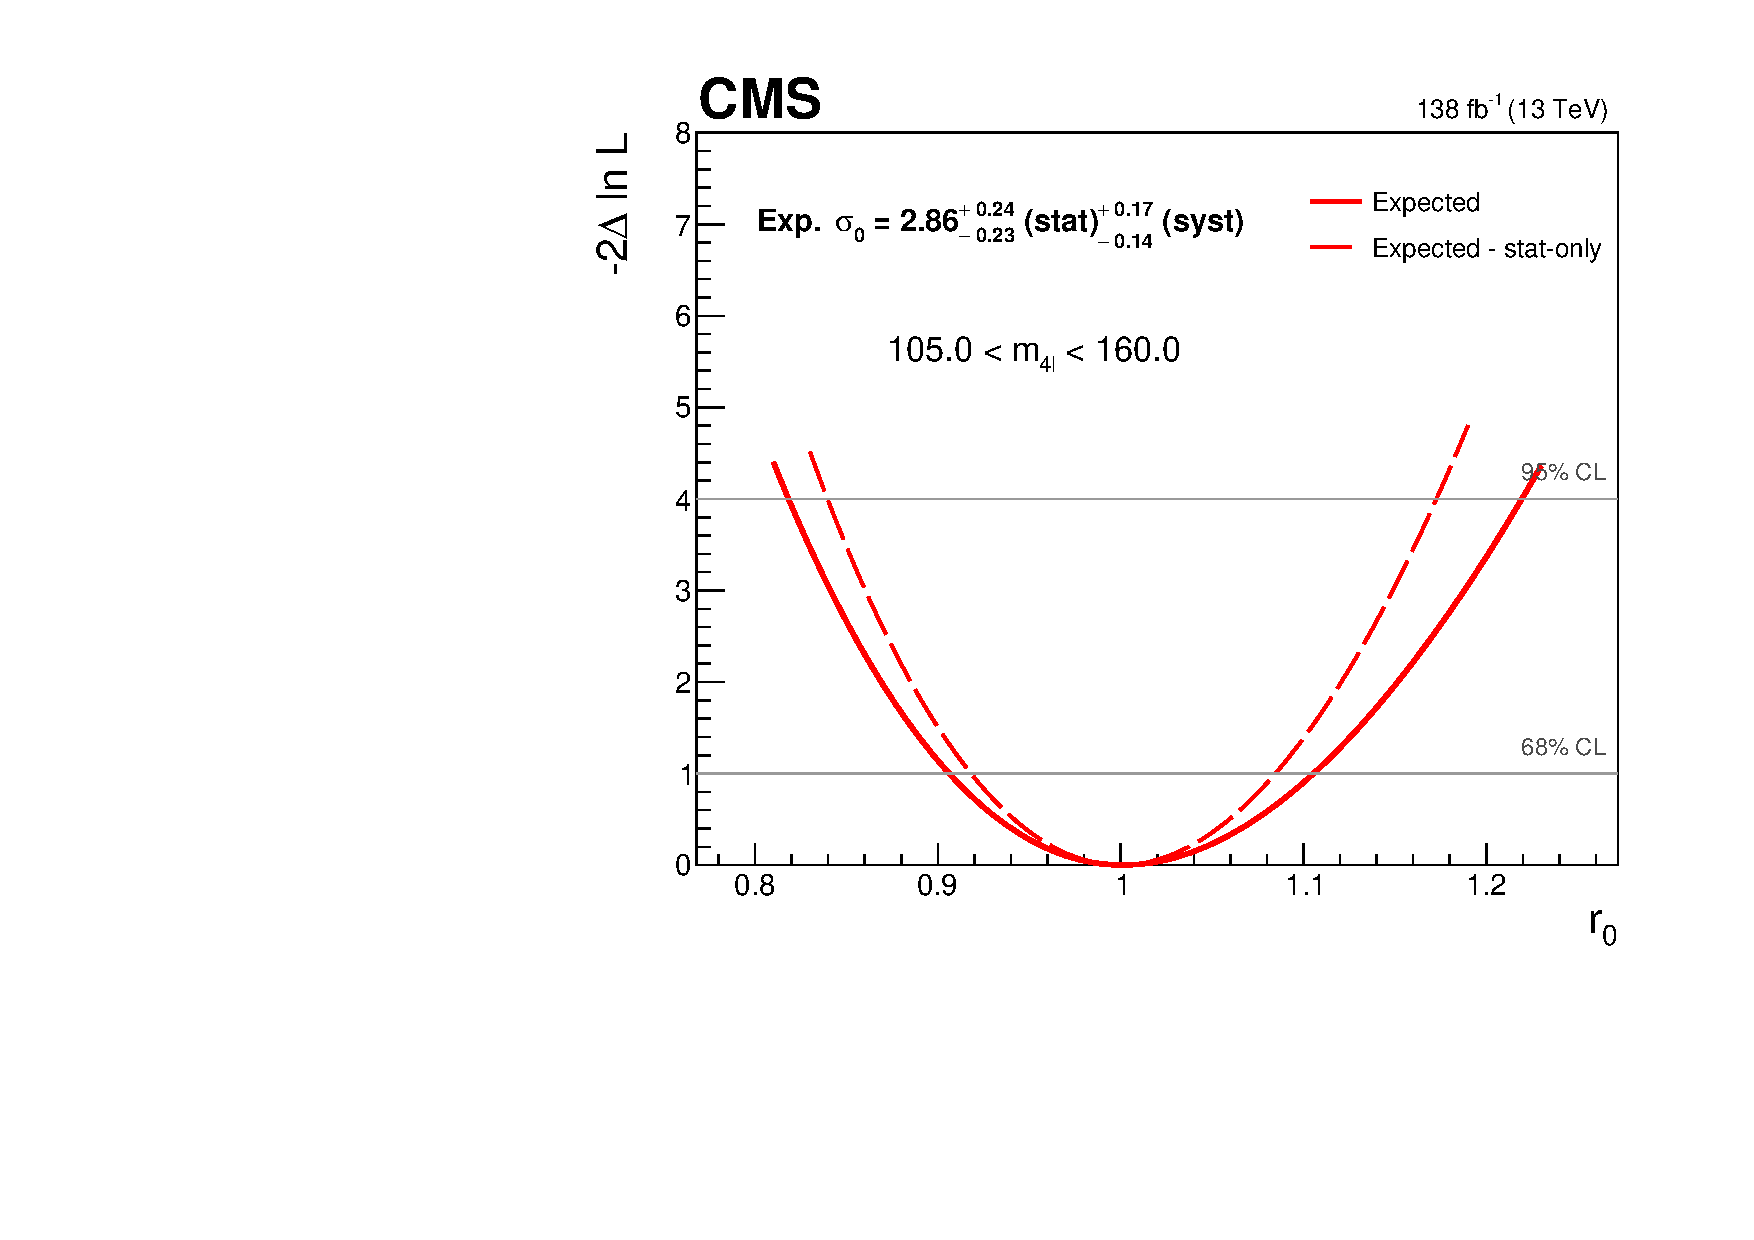
\includegraphics[width=0.5\textwidth]{Images/H4L/lhscan_compare_mass4l_SigmaBin0.pdf}
	\caption{
		Log likelihood scan for the measured inclusive fiducial cross section measurement.
		\label{fig:fiducial_LLScan}}
\end{figure}

\begin{figure}[!htb]
	\centering
	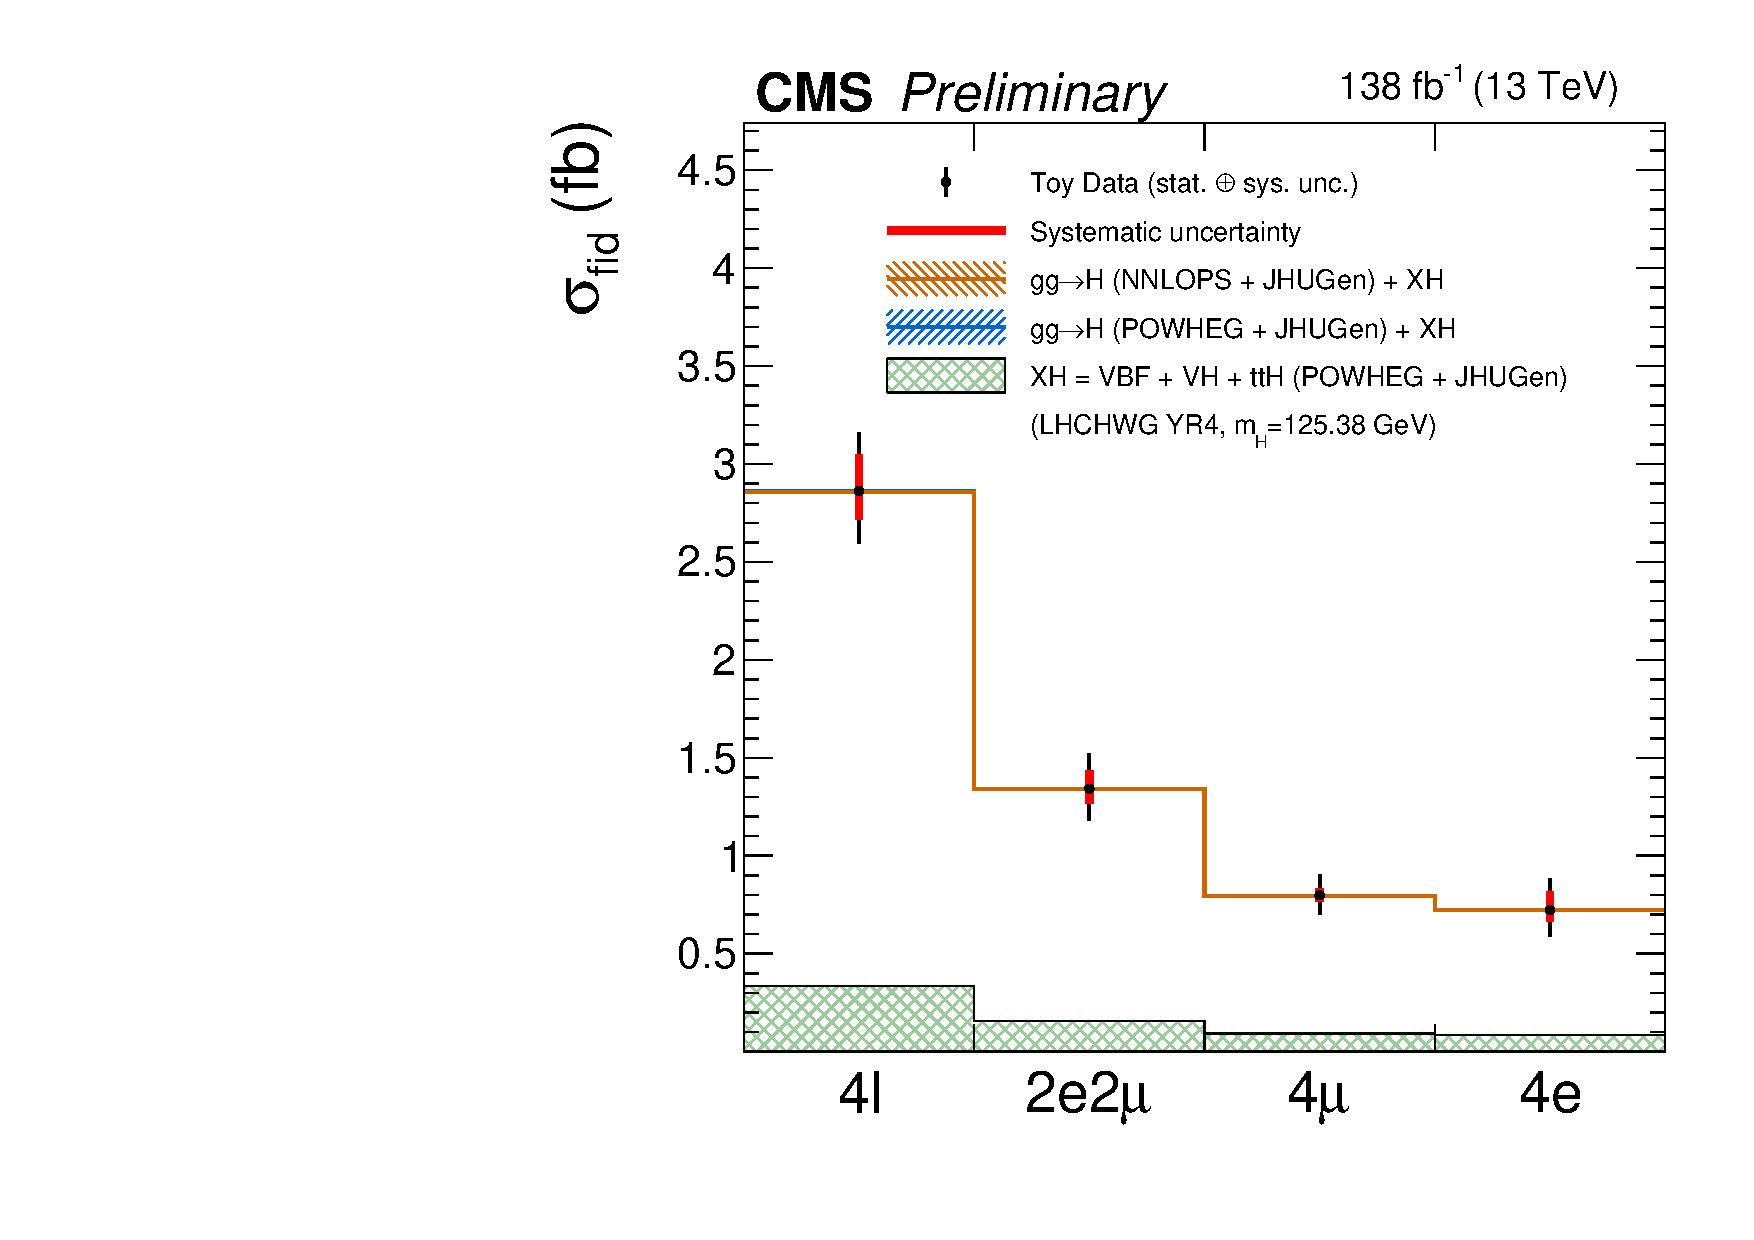
\includegraphics[width=0.48\textwidth]{Images/H4L/mass4l_unfoldwith_SM_125_asimov.pdf}
	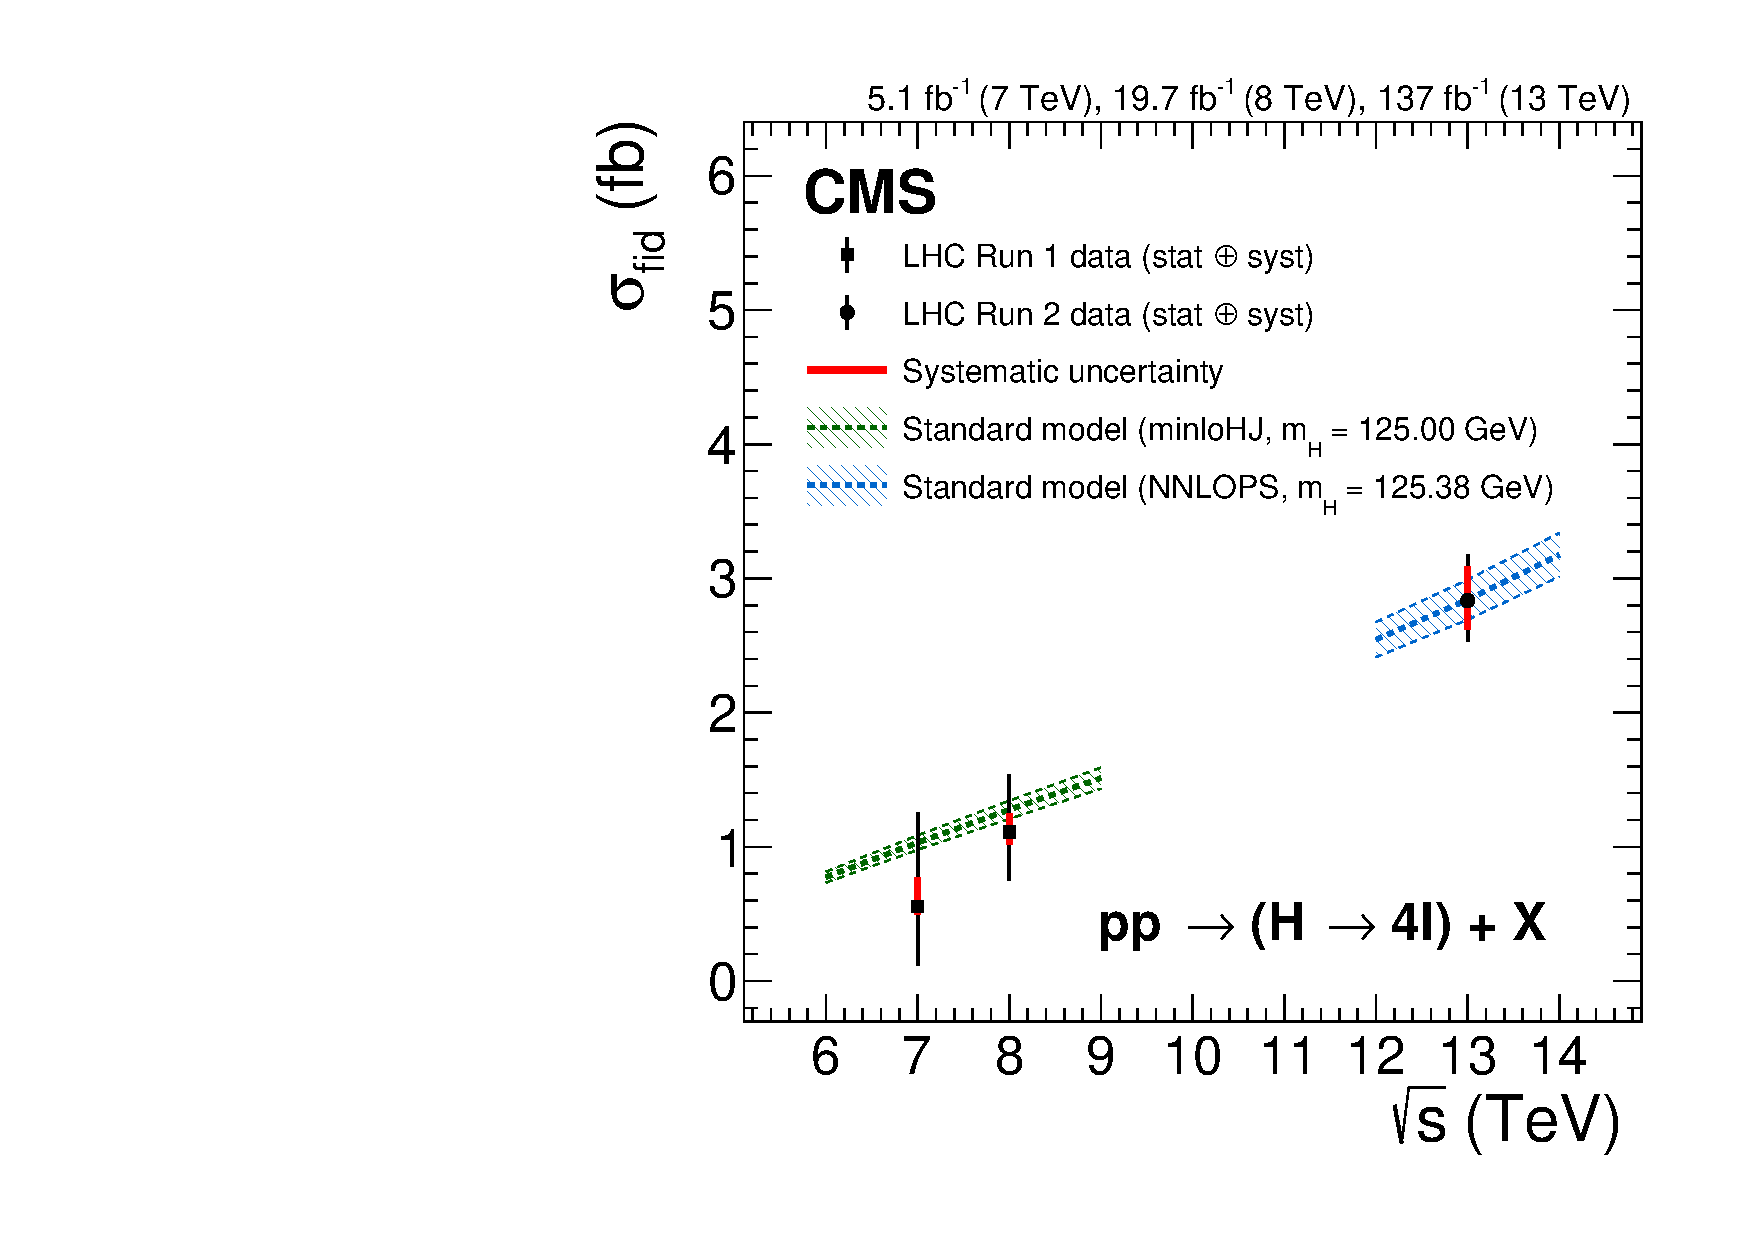
\includegraphics[width=0.48\textwidth]{Images/H4L/Figure_016-b.pdf}
	\caption{
		The measured inclusive fiducial cross section in different final states (\cmsLeft) and integrated as a function of $\sqrt{s}$ (\cmsRight).
		The acceptance is calculated using \POWHEG at  $\sqrt{s}=13\TeV$ and \textsc{HRes}~\cite{Grazzini:2013mca,deFlorian:2012mx}
		at $\sqrt{s}=$~7 and 8\TeV.
		\label{fig:fiducial_inclusive}}
\end{figure}

\begin{table*}[!htb]
	\centering
	\topcaption{
		The measured inclusive fiducial cross section and $\pm 1$ standard deviation uncertainties for different final states and data-taking periods at $\mH=125.38 \GeV$.
		The statistical and systematic uncertainties are given separately for the inclusive measurements.
		\label{tab:fiducial_inclusive}
	}
	\renewcommand{\arraystretch}{1.5}
	\begin{tabular}{ccccc}
		& $2\Pe 2\Pgm$~(fb) & $4\Pgm$~(fb) & $4\Pe$~(fb) & Inclusive (fb) \\
		\hline
		2016 & $X^{+Y}_{-Z}$ & $X^{+Y}_{-Z}$ & $X^{+Y}_{-Z}$ & $X^{+Y}_{-Z} = A\stat+B\syst$  \\
		2017 & $X^{+Y}_{-Z}$ & $X^{+Y}_{-Z}$ & $X^{+Y}_{-Z}$ & $X^{+Y}_{-Z} = A\stat+B\syst$   \\
		2018 & $X^{+Y}_{-Z}$ & $X^{+Y}_{-Z}$ & $X^{+Y}_{-Z}$ & $X^{+Y}_{-Z} = A\stat+B\syst$   \\
		2016--2018 & $1.34^{+0.18}_{-0.17}$ & $0.80^{+0.10}_{-0.10}$ & $0.72^{+0.16}_{-0.13}$ & $\obsXSECFid$   \\
	\end{tabular}
\end{table*}

%%%%%%%%%%%%%%%%%%%%%% Inclusive Fiducial XSEC: Float ZZ norm %%%%%%%%%%%%%%%%%%%%%%

The measurement of the inclusive fiducial cross section is repeated floating the normalisation of the \PZ\PZ$^\star$ irreducible background processes considered.
As explained in Sec.~\ref{sec:irrbkgd}, the normalisation of these processes is taken from MC simulation after applying dedicated scale factors to account for  NLO corrections in the theory predictions.
These corrections come with an associated uncertainty that may be reduced by a dedicated measurement of this normalisation using sidebands in data.
In addition, floating the normalisation of the irreducible background processes may enhance the model independence of the analysis.
The results are presented in Fig.~\ref{fig:fiducial_zzfloating} for the inclusive $\Hllll$ measurement as well as for the three final states considered. Fig.~\ref{fig:fiducial_zzfloating_corr} presents the corresponding correlation matrices.

\begin{figure}[!htb]
	\centering
	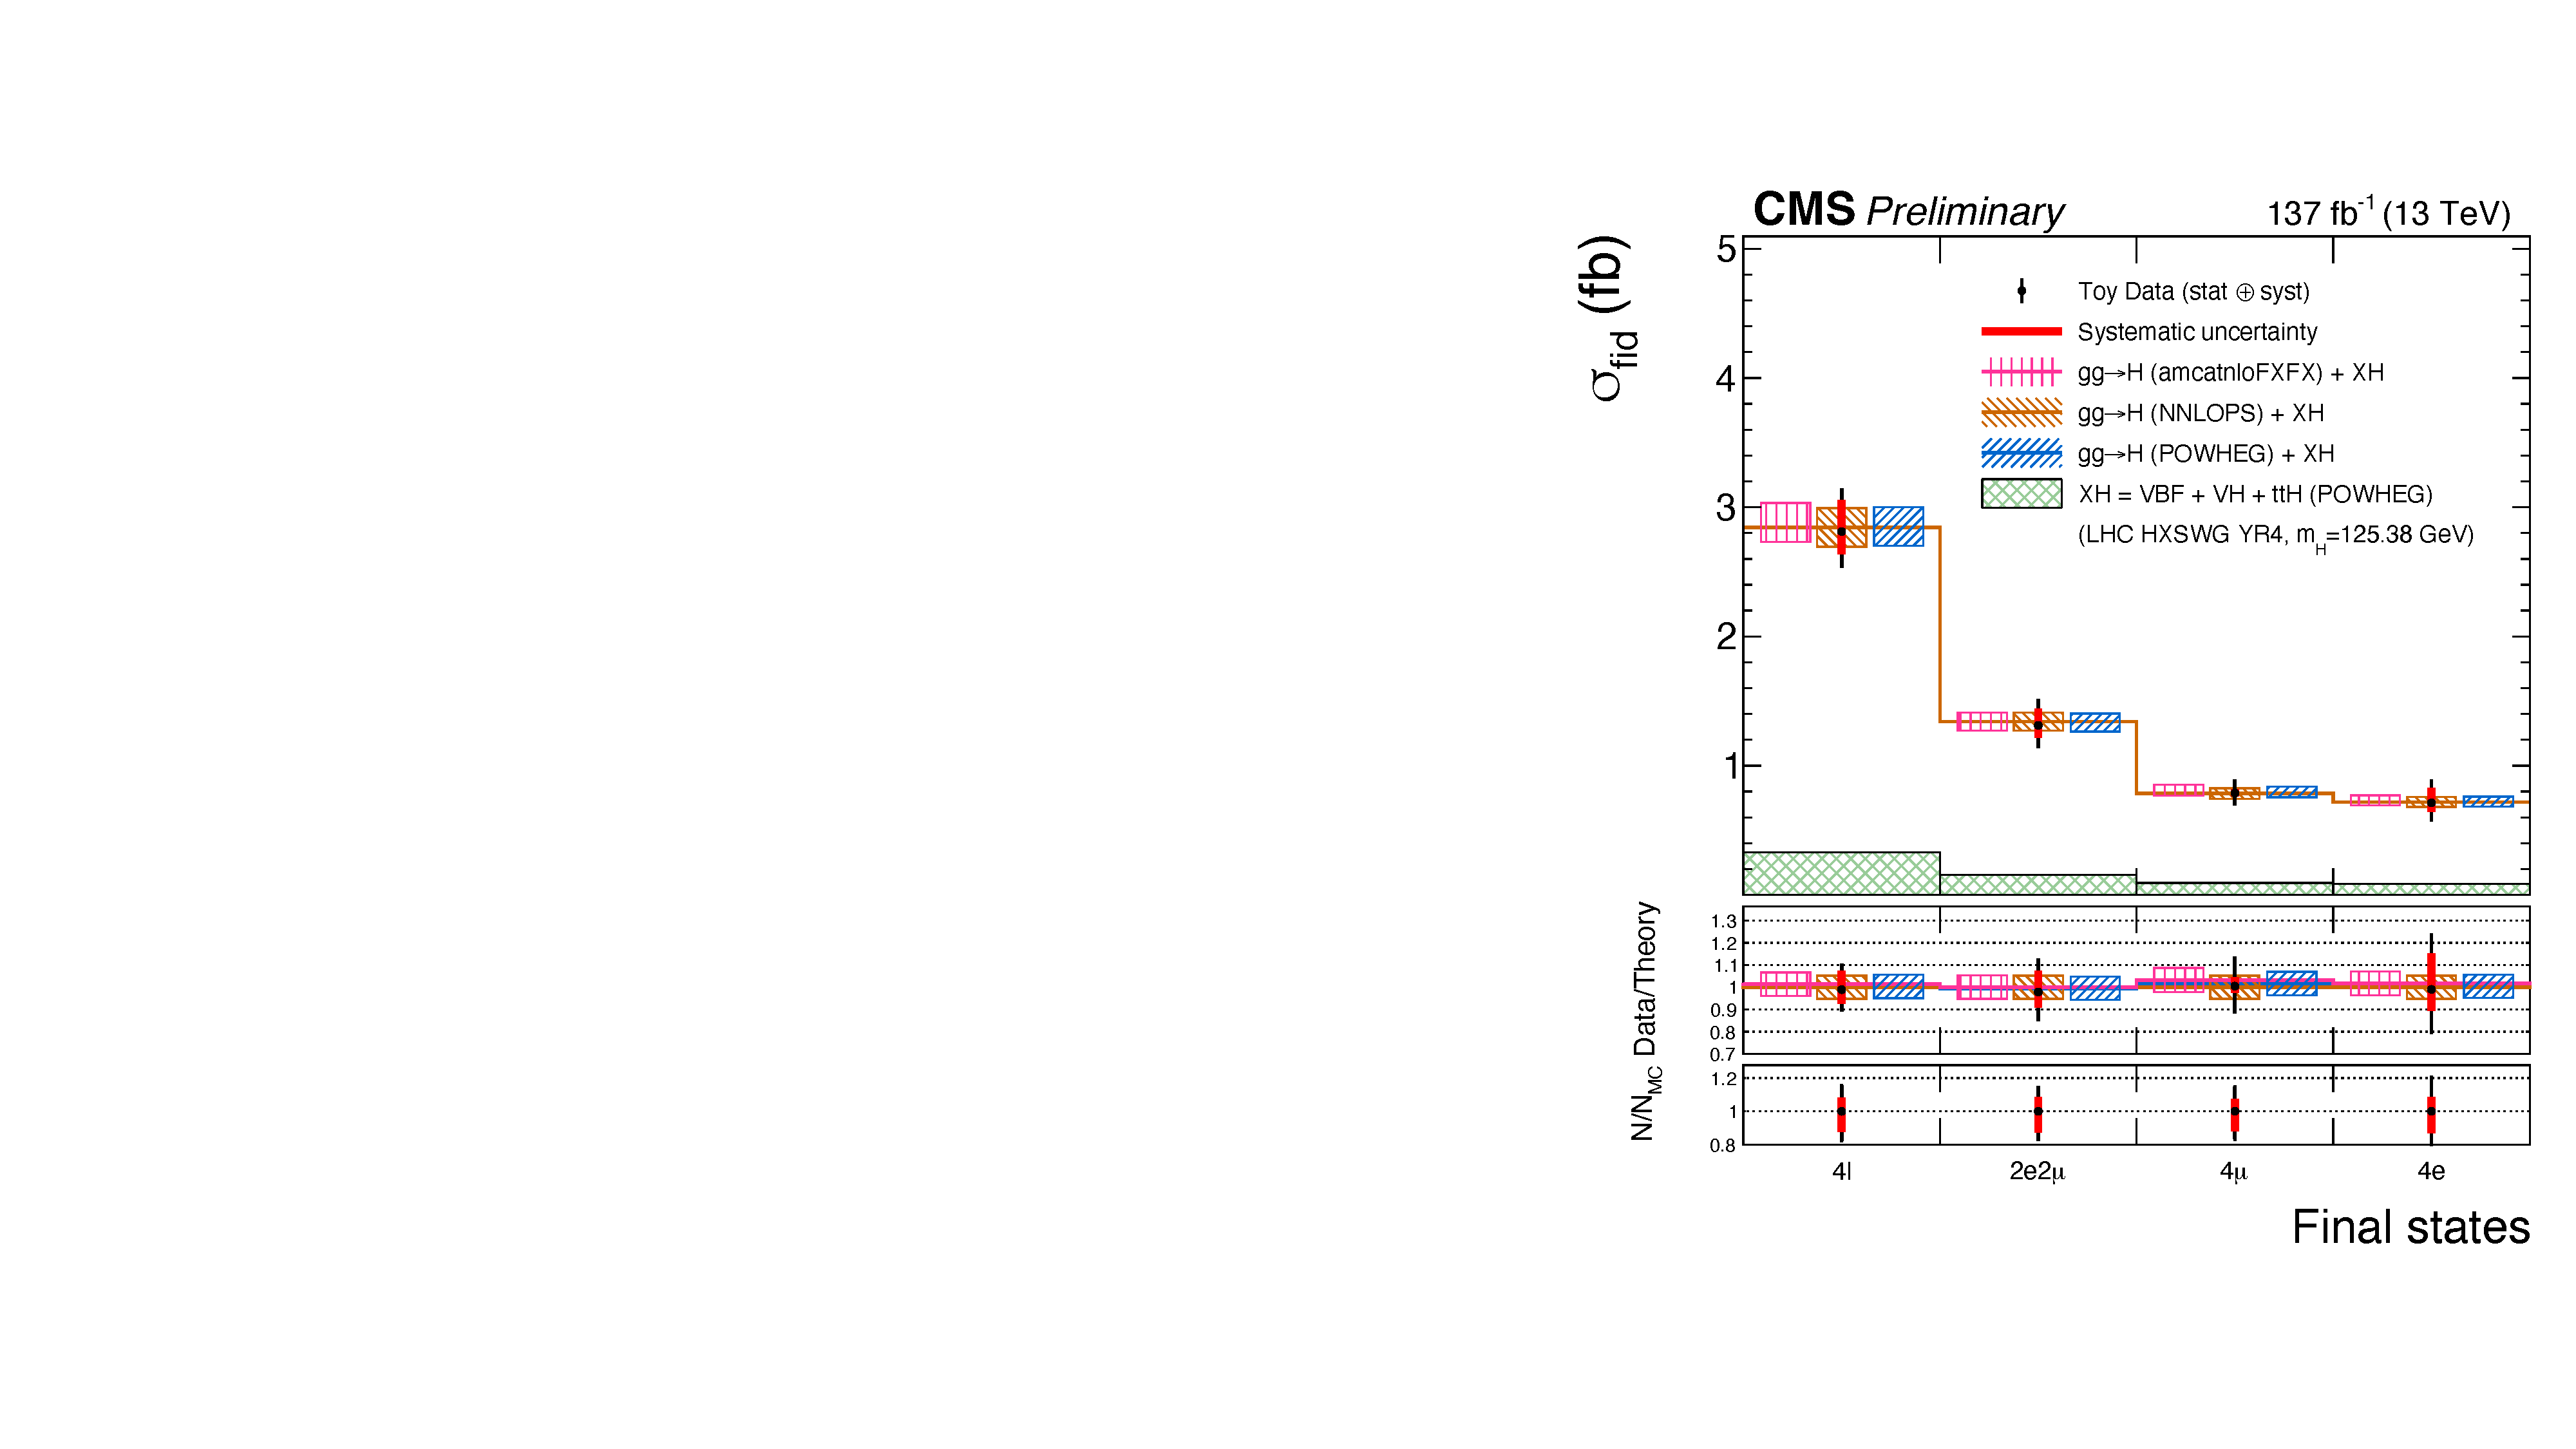
\includegraphics[width=0.5\textwidth]{Images/H4L/zznorm/mass4l_zzfloating_unfoldwith_SM_125_asimov_v1.pdf}
	\caption{
		The inclusive fiducial cross section measured in different final states with the irreducible backgrounds normalisation \PZ\PZ$^\star$  floating in the fit.
		The acceptance and theoretical uncertainties in the differential bins are calculated using the \POWHEG (blue), NNLOPS (orange), and MadGraph\_aMC@NLO (pink) generators.
        The sub-dominant component of the signal ($\VBF + \VH + \ttH$) is denoted as XH and it is fixed to the SM.
        The ratio to the theoretical prediction obtained from each generator is shown in the central panel, while the bottom panel shows the ration between the measured \PZ\PZ$^\star$ normalisation and the prediction from MC.
		\label{fig:fiducial_zzfloating}}
\end{figure}

\begin{figure}[!htb]
	\centering
	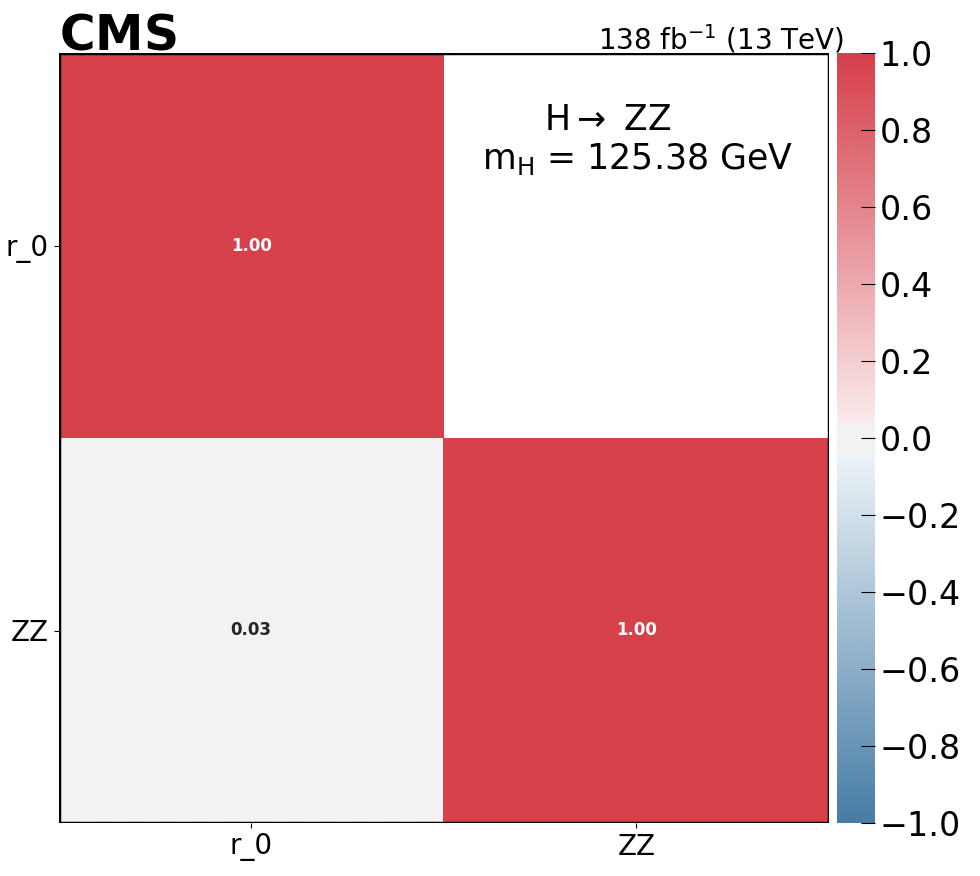
\includegraphics[width=0.48\textwidth]{Images/H4L/zznorm/corr_m4l_v3.png}
	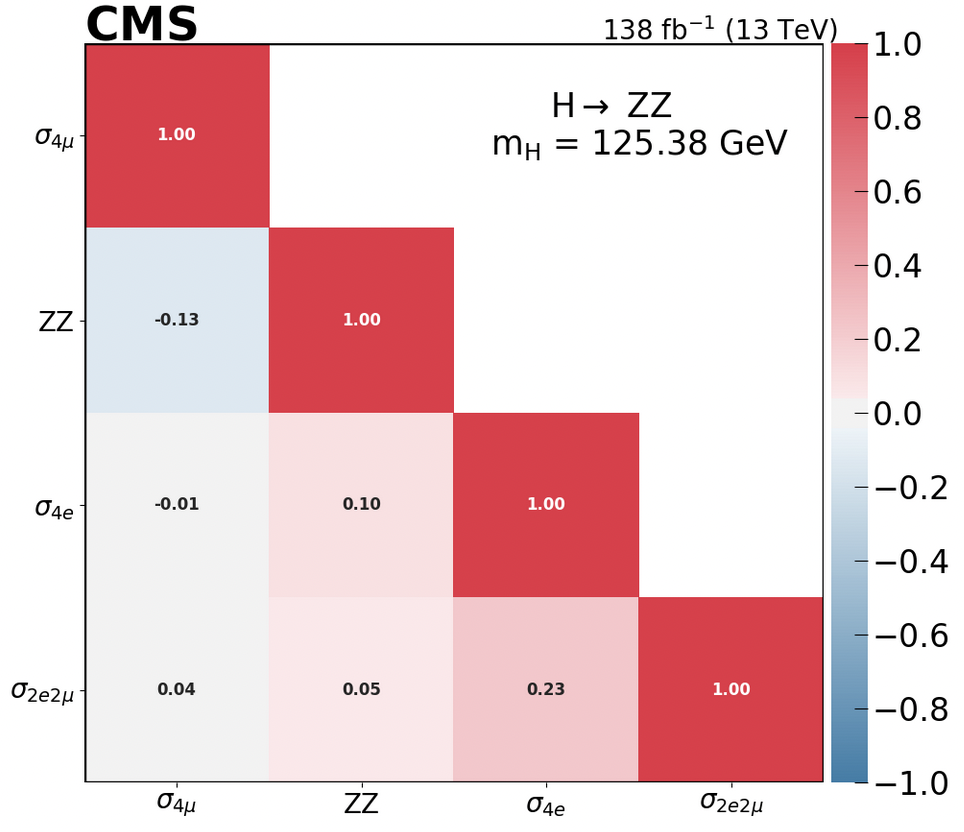
\includegraphics[width=0.48\textwidth]{Images/H4L/zznorm/corr_m4l_v2.png}
	\caption{
		Correlation matrices between the inclusive fiducial cross section and the \PZ\PZ$^\star$ normalisation (left). Correlations between the fiducial cross sections in each final state and the \PZ\PZ$^\star$ normalisation (right).
		\label{fig:fiducial_zzfloating_corr}}
\end{figure}


Tab.~\ref{tab:fiducial_zzfloat} summarises the measured cross sections and \PZ\PZ$^\star$ normalisation.
No large correlation is observed between the different fiducial cross sections and the \PZ\PZ$^\star$ normalisation.
The measured cross sections are found to be in agreement with the results obtained when the irreducible background normalisation is extracted from MC simulation and fixed to the SM expecation in the measurement.
In addition, the uncertainty on this parameter, when it is extracted from a fit of the data sidebands, is found to be larger than the theoretical uncertainty on its predictions.
For all these reasons, in the following the \PZ\PZ$^\star$ normalisation is taken from MC without introducing any model depdence or worsening of the analysis performance.

\begin{table*}[!htb]
	\centering
	\topcaption{
		The measured inclusive fiducial cross section and $\pm 1$ standard deviation uncertainties for different final states and data-taking periods at $\mH=125.38 \GeV$.
		The statistical and systematic uncertainties are given separately for the inclusive measurements.
		\label{tab:fiducial_zzfloat}
	}
	\renewcommand{\arraystretch}{1.5}
	\begin{tabular}{ccccc}
		& $2\Pe 2\Pgm$~(fb) & $4\Pgm$~(fb) & $4\Pe$~(fb) & Inclusive (fb) \\
		\hline
		$\sigma_{{\mathrm{fid}}} $& $1.34^{+0.18}_{-0.16}$ & $0.80^{+0.11}_{-0.10}$ & $0.72^{+0.16}_{-0.14}$ &  $2.86^{+0.23}_{-0.22}\stat^{+0.18}_{-0.15}\syst \unit{fb}$  \\
		 \PZ\PZ$^\star$ norm. & $410^{+40}_{-50}$ & $410^{+40}_{-50}$ & $410^{+40}_{-50}$ & $410^{+40}_{-50}$   \\
	\end{tabular}
\end{table*}

%\clearpage

\subsection{Differential cross sections: production}
Fiducial cross sections are measured in differential bins of variables sensitive to the production side in the $\HZZfl$ channel.
The results for the transverse momentum and rapidity of the Higgs boson are shown in Fig.~\ref{fig:fidPTH},\ref{fig:fidYH}, respectively.
% Fig.~\ref{fig:fidNJ},\ref{fig:fidPTJ1},\ref{fig:fidPTJ2} show the measurements of the fiducial cross sections in differential bins of jet-related observables, namely: the number of associated jets in the event and the transverse momentum of the leading and sub-leading jet in the event.
% The fiducial cross section is also measured in bins of the inveriant mass of the dijet system, as shown in Fig.~\ref{fig:fidMJJ}. This measurement, performed for the first time in the $4\ell$ channel, allows to enhance the sensitivity of the analysis to phase space regions of $\VBF$ and $\ttH$ production mechanisms, where a larger jet-multiplicity is expected.

% This analysis presents also the results for the cross sections measured in bins of observables of the \PH+j and \PH+jj systems. These results meet the constantly increasing interest from the theory community, as they allow to probe the QCD emission pattern with experimental data.
% The measurements of the fiducial cross section in differential bins of the invariant mass and transverse momentum of the \PH+j system are presented in Fig.~\ref{fig:fidMHJ} and \ref{fig:fidPTHJ}, respectively, while Fig.~\ref{fig:fidPTHJJ} shows the results in differential bins of the transverse momentum of the \PH+jj system.

% With the same goal of enhancing the sensitivity to phase space regions that probe directly the departure from LO kinematics and thus the QCD emission pattern, the cross sections in differential bins of the rapidity-weighted jet-vetoes introduced in Sec.~\ref{sec:observables} are also measured. Fig.~\ref{fig:fidTC} presents the results for  $\mathcal{T}_{\text{C}}$, while the results for  $\mathcal{T}_{\text{B}}$ are shown in Fig.~\ref{fig:fidTB}.

% %\clearpage

\begin{center}
	\begin{figure}[!htbp]
		\centering
		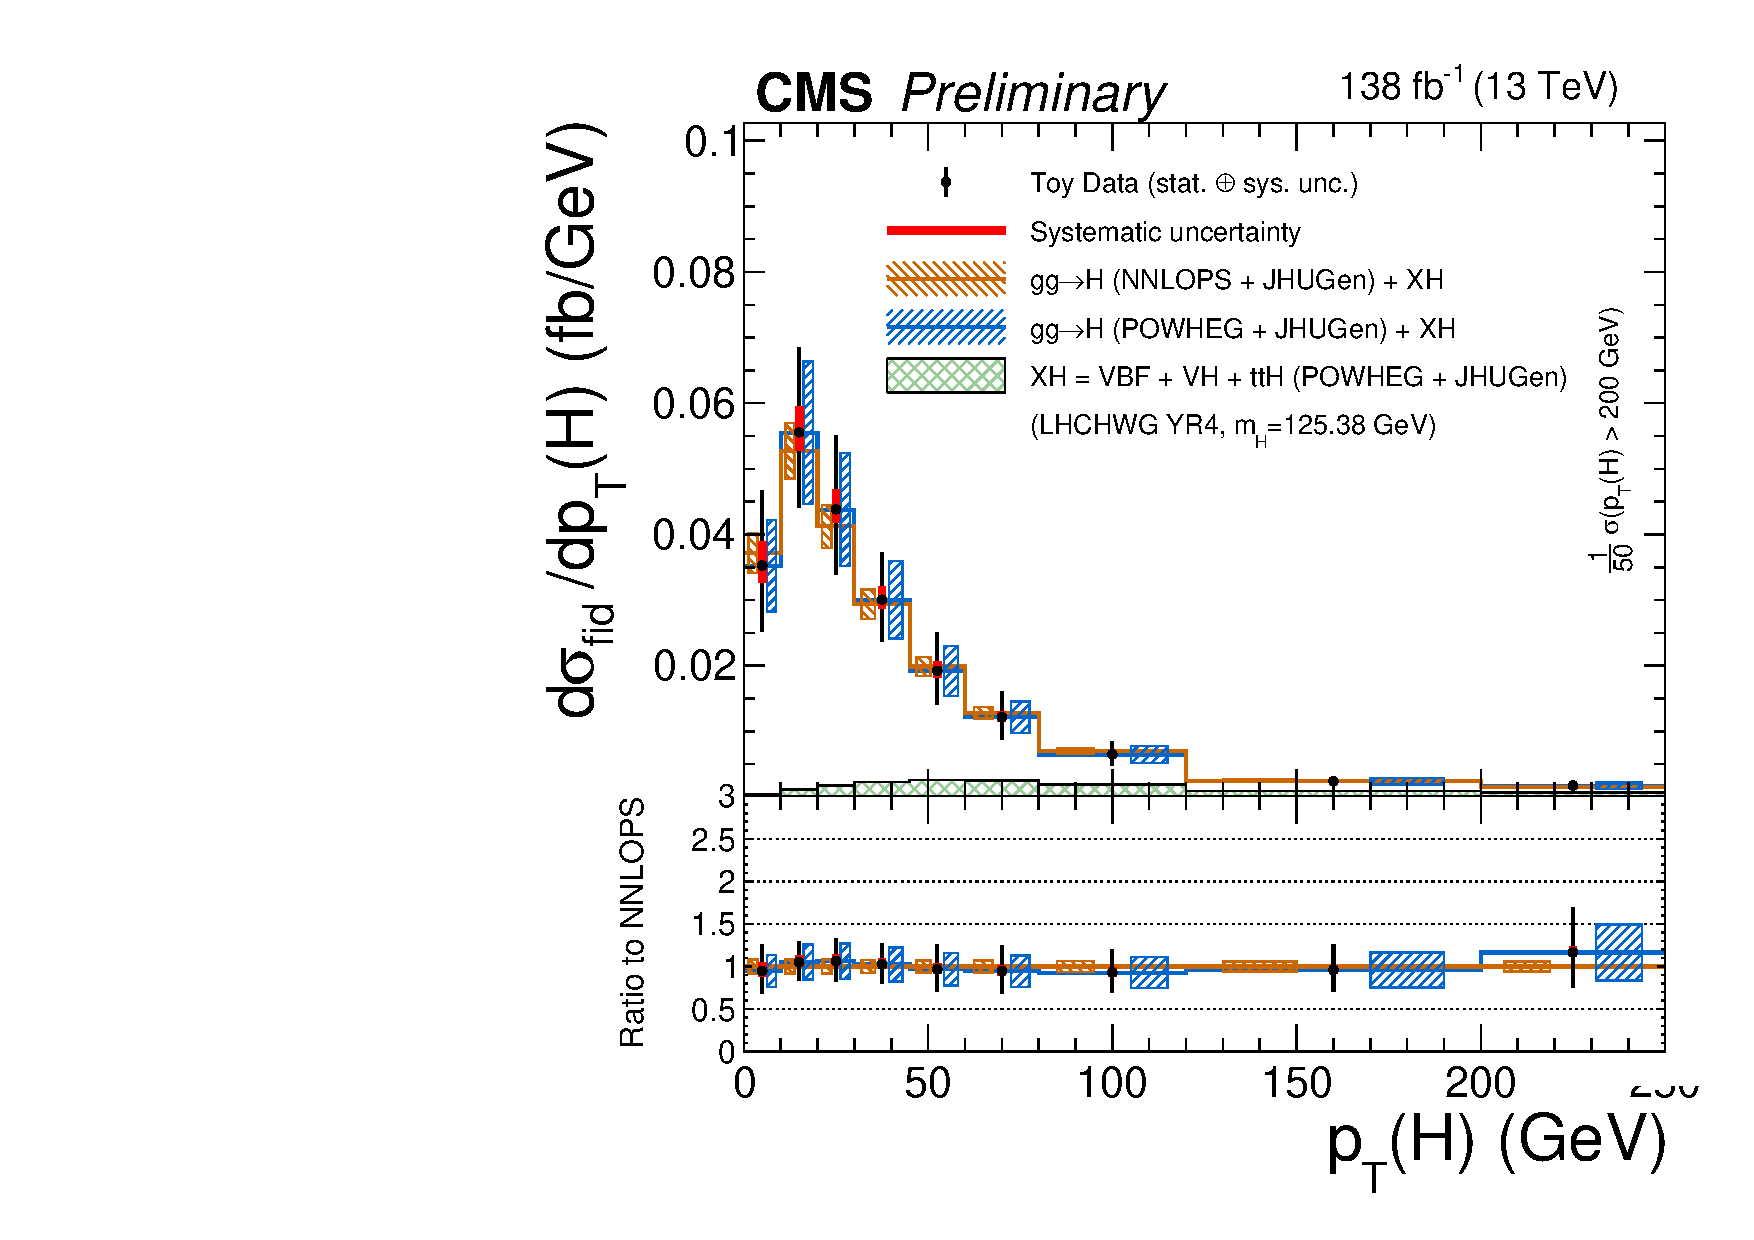
\includegraphics[width=0.48\textwidth]{Images/H4L/pT4l_unfoldwith_SM_125_asimov.pdf}
		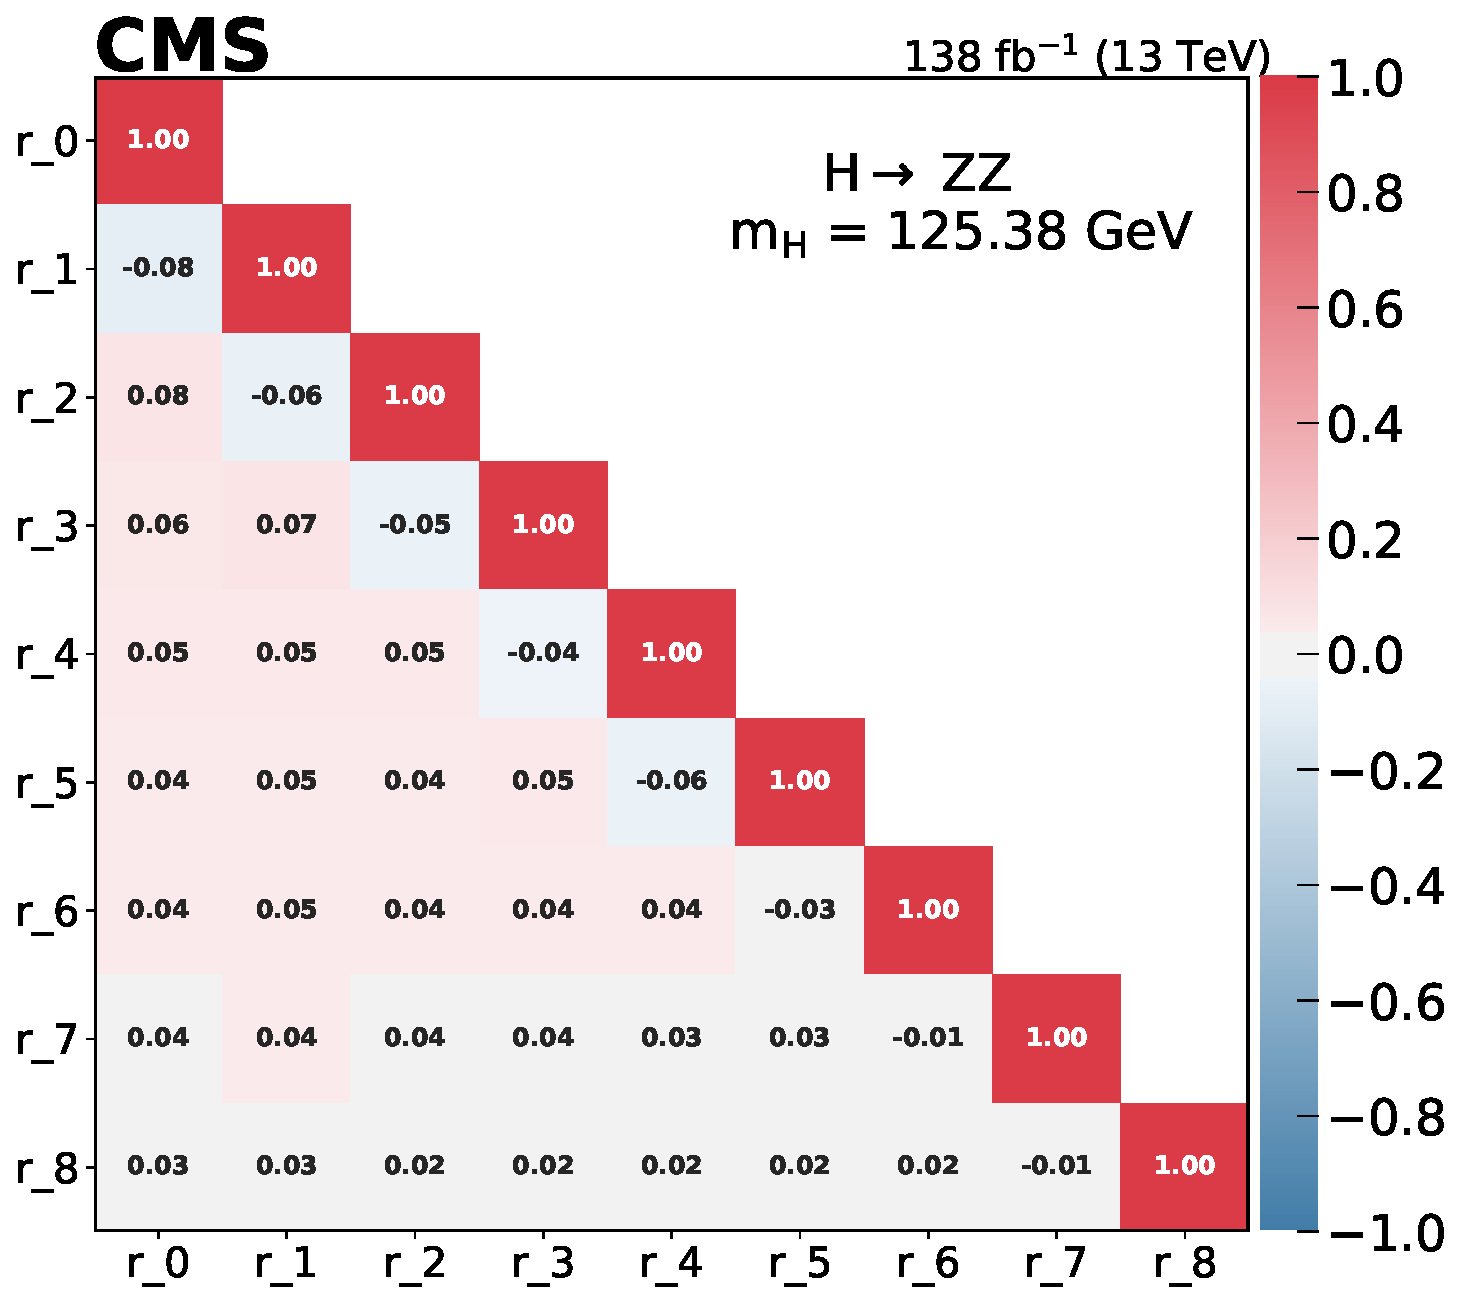
\includegraphics[width=0.48\textwidth]{Images/H4L/correlations/corr_pT4l_v3.pdf}\\
		\caption{
			Differential cross sections as a function of the transverse momentum of the Higgs boson $\pt^{\PH}$ (left) and the correlation matrix between the observed differential cross sections (right). 
			The acceptance and theoretical uncertainties in the differential bins are calculated using the $\ggH$ predictions from the \POWHEG generator (blue) normalised to $\mathrm{N^3LO}$.
			The sub-dominant component of the signal ($\VBF + \VH + \ttH$) is denoted as XH and are fixed to the SM.
			The measured cross sections are also compared with the ggH predictions from the NNLOPS (orange) and MadGraph\_aMC@NLO (pink) generators.
			The black points represent the measured fiducial cross sections in each bin, while the black error bars represent the total uncertainty on each measurement.
			The red boxes depict the systematic components of the uncertainties introduced in Sec.~\ref{sec:systematics}.
			\label{fig:fidPTH}}
	\end{figure}
\end{center}

%\clearpage

\begin{center}
	\begin{figure}[!htbp]
		\centering
		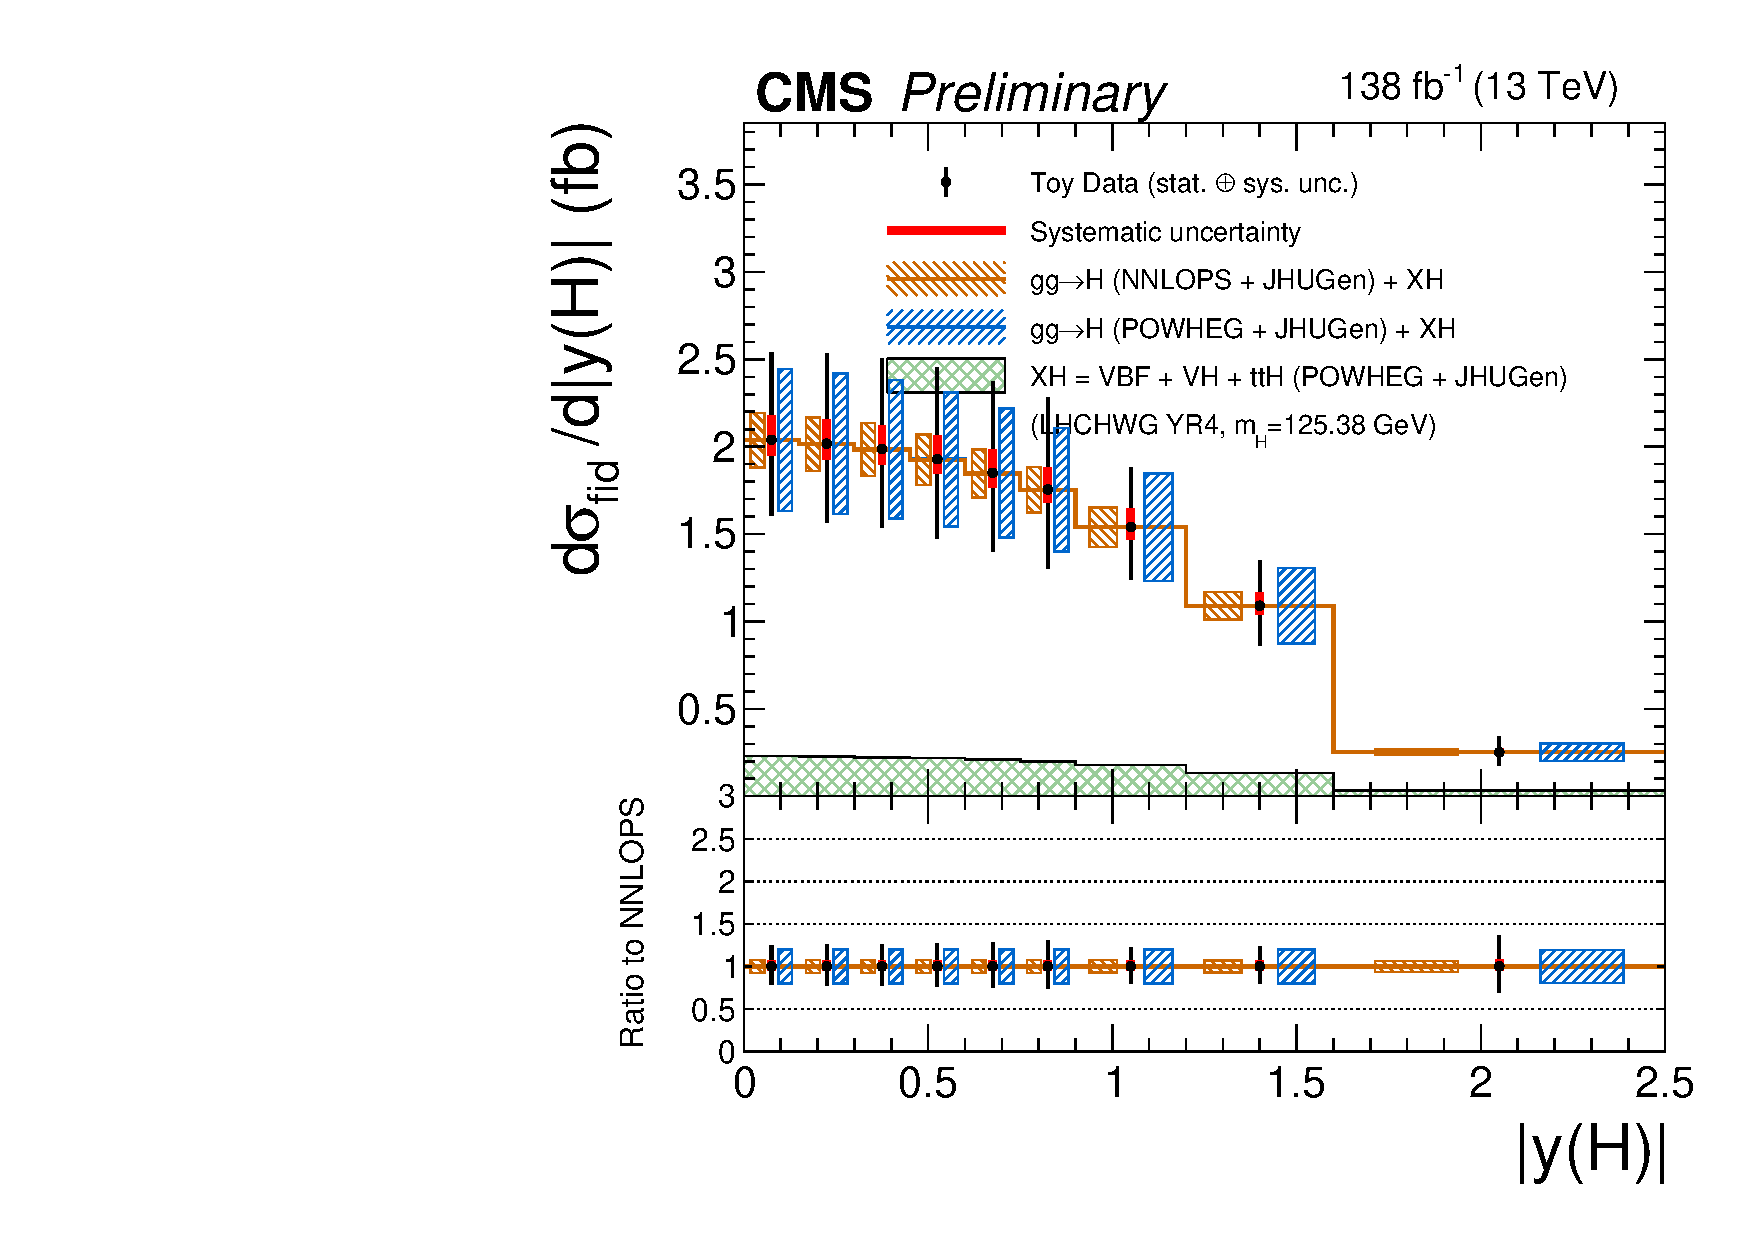
\includegraphics[width=0.48\textwidth]{Images/H4L/rapidity4l_unfoldwith_SM_125_asimov.pdf}
		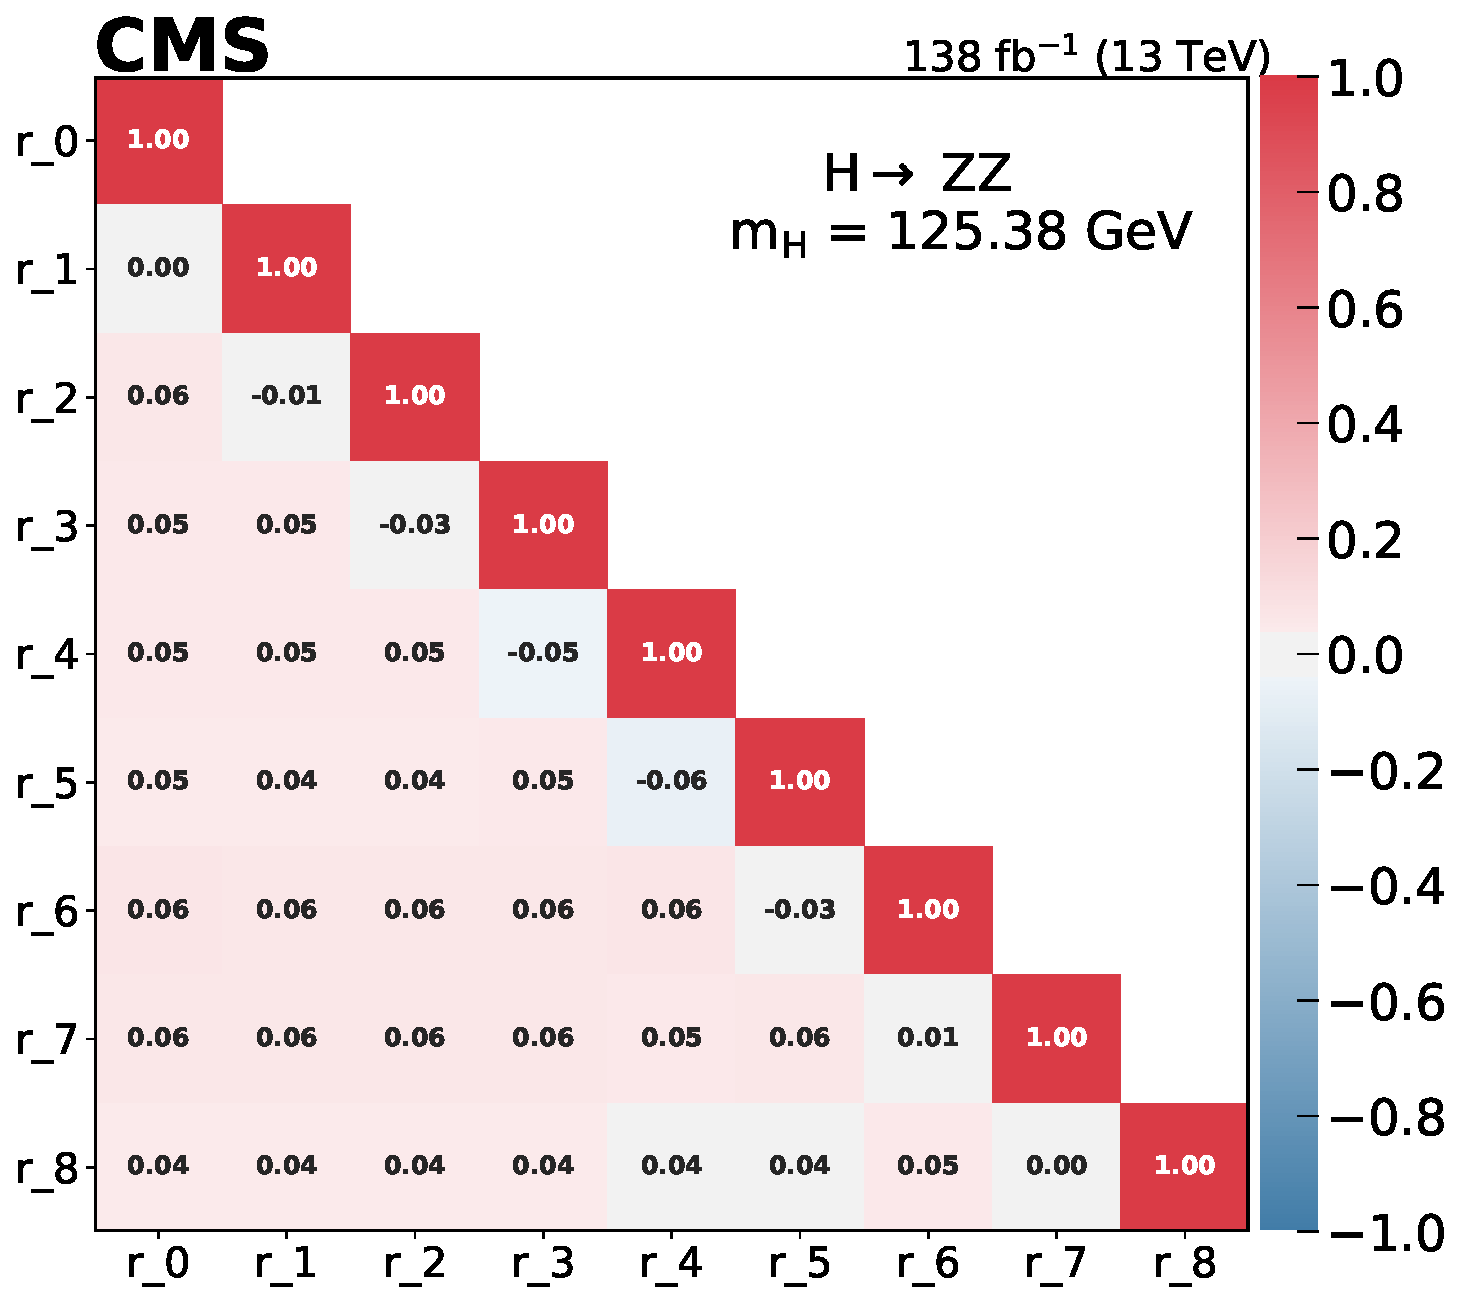
\includegraphics[width=0.48\textwidth]{Images/H4L/correlations/corr_rapidity4l_v3.pdf}\\
		\caption{
			Differential cross sections as a function of  the rapidity of the Higgs boson $\abs{y^{\PH}}$ (left) and the correlation matrix between the observed differential cross sections (right).
			The acceptance and theoretical uncertainties in the differential bins are calculated using the \POWHEG (blue), NNLOPS (orange), and MadGraph\_aMC@NLO (pink) generators.
			The sub-dominant component of the signal ($\VBF + \VH + \ttH$) is denoted as XH and it is fixed to the SM.
			\label{fig:fidYH}}
	\end{figure}
\end{center}

%\clearpage

% \begin{center}
% 	\begin{figure}[!htb]
% 		\centering
% 		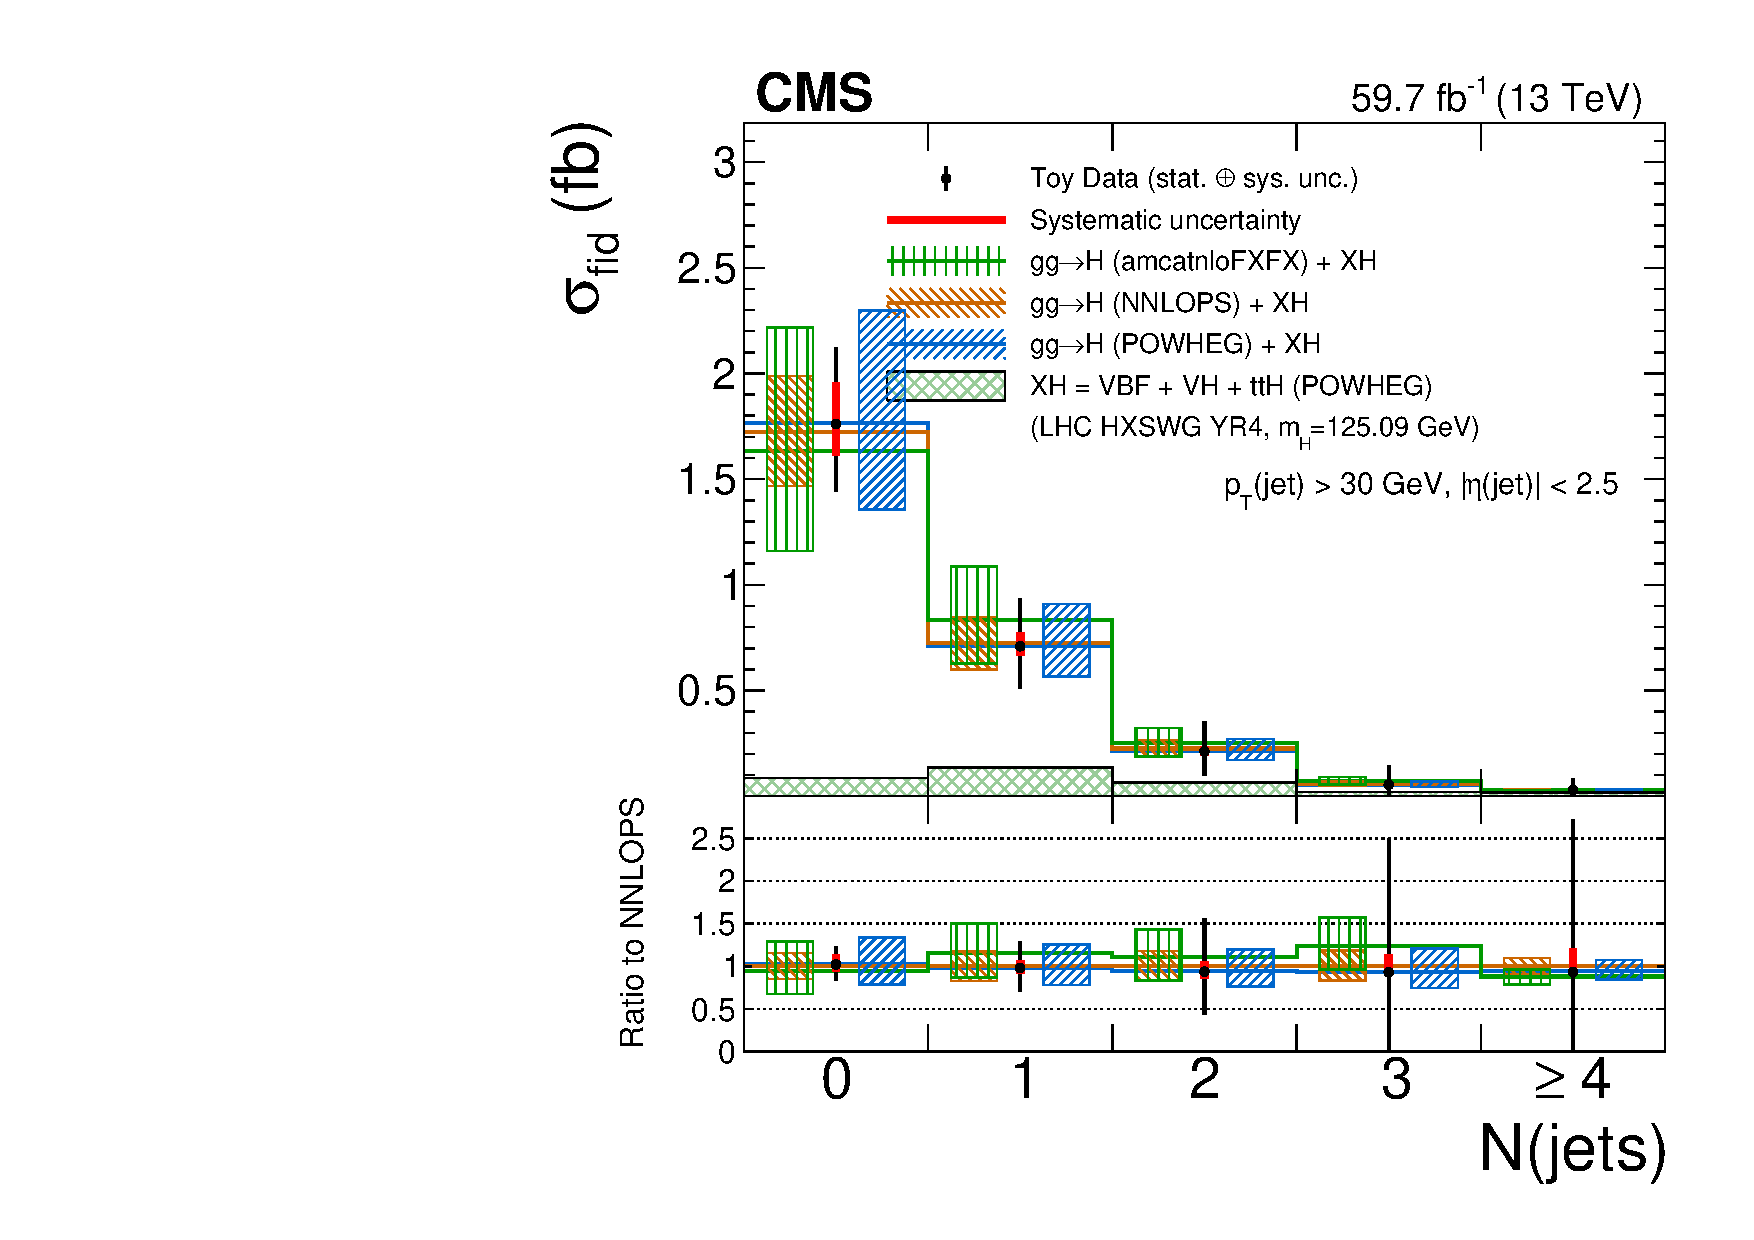
\includegraphics[width=0.48\textwidth]{Images/H4L/njets_pt30_eta2p5_unfoldwith_SM_125_asimov.pdf}
% 		\includegraphics[width=0.48\textwidth]{Images/H4L/correlations/corr_njets_pt30_eta4p7_v3.pdf}\\
% 		\caption{
% 			Differential cross sections as a function of the number of associated jets in the event (left) and the correlation matrix between the observed differential cross sections (right).
% 			The acceptance and theoretical uncertainties in the differential bins are calculated using the \POWHEG (blue), NNLOPS (orange), and MadGraph\_aMC@NLO (pink) generators.
% 			The sub-dominant component of the signal ($\VBF + \VH + \ttH$) is denoted as XH and it is fixed to the SM.
% 			\label{fig:fidNJ}}
% 	\end{figure}
% \end{center}

%\clearpage

% \begin{center}
% 	\begin{figure}[!htb]
% 		\centering
% 		\includegraphics[width=0.48\textwidth]{Images/H4L/pTj1_unfoldwith_SM_125_asimov.pdf}
% 		\includegraphics[width=0.48\textwidth]{Images/H4L/correlations/corr_pTj1_v3.pdf}\\
% 		\caption{
% 			Differential cross sections as a function of the \pt of the leading jet in the event (left) and the correlation matrix between the observed differential cross sections (right).
% 			The acceptance and theoretical uncertainties in the differential bins are calculated using the \POWHEG (blue), NNLOPS (orange), and MadGraph\_aMC@NLO (pink) generators.
% 			The sub-dominant component of the signal ($\VBF + \VH + \ttH$) is denoted as XH and it is fixed to the SM.
% 			\label{fig:fidPTJ1}}
% 	\end{figure}
% \end{center}

%\clearpage

% \begin{center}
% 	\begin{figure}[!htb]
% 		\centering
% 		\includegraphics[width=0.48\textwidth]{Images/H4L/pTj2_unfoldwith_SM_125_logscale_asimov.pdf}	\includegraphics[width=0.48\textwidth]{Images/H4L/correlations/corr_pTj2_v3.pdf}\\
% 		\caption{
% 			Differential cross sections as a function of the \pt of the sub-leading jet in the event (left) and the correlation matrix between the observed differential cross sections (right).
% 			The acceptance and theoretical uncertainties in the differential bins are calculated using the \POWHEG (blue), NNLOPS (orange), and MadGraph\_aMC@NLO (pink) generators.
% 			The sub-dominant component of the signal ($\VBF + \VH + \ttH$) is denoted as XH and it is fixed to the SM.
% 			\label{fig:fidPTJ2}}
% 	\end{figure}
% \end{center}

% %\clearpage

% %%%%%%%%%%%%%%%%%%%%%%%% Dijet system %%%%%%%%%%%%%%%%%%%%%%%%%

% \begin{center}
% 	\begin{figure}[!htb]
% 		\centering
% 		\includegraphics[width=0.48\textwidth]{Images/H4L/mjj_unfoldwith_SM_125_logscale_asimov.pdf}	\includegraphics[width=0.48\textwidth]{Images/H4L/correlations/corr_mjj_v3.pdf}\\
% 		\caption{
% 			Differential cross sections as a function of the invariant mass of the di-jet system $m_{jj}$ (left) and the correlation matrix between the observed differential cross sections (right).
% 			The first bin comprises all those events with less than two jets, for which $m_{jj}$  is undefined.
% 			The acceptance and theoretical uncertainties in the differential bins are calculated using the \POWHEG (blue), NNLOPS (orange), and MadGraph\_aMC@NLO (pink) generators.
% 			The sub-dominant component of the signal ($\VBF + \VH + \ttH$) is denoted as XH and it is fixed to the SM.
% 			\label{fig:fidMJJ}}
% 	\end{figure}
% \end{center}

% %\clearpage


% %%%%%%%%%%%%%%%%%%%%%%%% Dijet system %%%%%%%%%%%%%%%%%%%%%%%%%

% \begin{center}
% 	\begin{figure}[!htb]
% 		\centering
% 		\includegraphics[width=0.48\textwidth]{Images/H4L/mHj_unfoldwith_SM_125_asimov.pdf}
% 		\includegraphics[width=0.48\textwidth]{Images/H4L/correlations/corr_mHj_v3.pdf}\\
% 		\caption{
% 			Differential cross sections as a function of the invariant mass of the \PH+leading-jet system $m_{\PH j}$ (left) and the correlation matrix between the observed differential cross sections (right).
% 			The first bin comprises all those events with less than one jet, for which $m_{\PH j}$  is undefined.
% 			The acceptance and theoretical uncertainties in the differential bins are calculated using the \POWHEG (blue), NNLOPS (orange), and MadGraph\_aMC@NLO (pink) generators.
% 			The sub-dominant component of the signal ($\VBF + \VH + \ttH$) is denoted as XH and it is fixed to the SM.
% 			\label{fig:fidMHJ}}
% 	\end{figure}
% \end{center}

% %\clearpage

% \begin{center}
% 	\begin{figure}[!htb]
% 		\centering
% 		\includegraphics[width=0.48\textwidth]{Images/H4L/pTHj_unfoldwith_SM_125_logscale_asimov.pdf}
% 		\includegraphics[width=0.48\textwidth]{Images/H4L/correlations/corr_pTHj_v3.pdf}\\
% 		\caption{
% 			Differential cross sections as a function of the transverse momentum of the \PH+leading-jet system $\pt^{\PH j}$ (left) and the correlation matrix between the observed differential cross sections (right).
% 			The first bin comprises all those events with less than one jet, for which $\pt^{\PH j}$  is undefined.
% 			The acceptance and theoretical uncertainties in the differential bins are calculated using the \POWHEG (blue), NNLOPS (orange), and MadGraph\_aMC@NLO (pink) generators.
% 			The sub-dominant component of the signal ($\VBF + \VH + \ttH$) is denoted as XH and it is fixed to the SM.
% 			\label{fig:fidPTHJ}}
% 	\end{figure}
% \end{center}

%\clearpage

%\begin{center}
%\begin{figure}[!htb]
%	\centering
%	\includegraphics[width=0.48\textwidth]{Images/H4L/plot_njets_pt30_eta2p5_mHjj.png}
%	\includegraphics[width=0.48\textwidth]{Images/H4L/correlations/corr_mHjj_v3.pdf}\\
%	\caption{
	%		Differential cross sections as a function of  $m_{\PH jj}$.
	%		The acceptance and theoretical uncertainties in the differential bins are calculated using \POWHEG.
	%		The sub-dominant component of the signal ($\VBF + \VH + \ttH$) is denoted as XH.
	%		\label{fig:fidMHJJ}}
%\end{figure}
%\end{center}

% \begin{center}
% 	\begin{figure}[!htb]
% 		\centering
% 		\includegraphics[width=0.48\textwidth]{Images/H4L/pTHjj_unfoldwith_SM_125_asimov.pdf}
% 		\includegraphics[width=0.48\textwidth]{Images/H4L/correlations/corr_pTHjj_v3.pdf}\\
% 		\caption{
% 			Differential cross sections as a function of the transverse momentum of the \PH+di-jet system $\pt^{\PH jj}$ (left) and the correlation matrix between the observed differential cross sections (right).
% 			The first bin comprises all those events with less than two jet, for which $\pt^{\PH jj}$  is undefined.
% 			The acceptance and theoretical uncertainties in the differential bins are calculated using the \POWHEG (blue), NNLOPS (orange), and MadGraph\_aMC@NLO (pink) generators.
% 			The sub-dominant component of the signal ($\VBF + \VH + \ttH$) is denoted as XH and it is fixed to the SM.
% 			\label{fig:fidPTHJJ}}
% 	\end{figure}
% \end{center}

%\clearpage

%%%%%%%%%%%%%%%%%%%%%%%% Jet Veto T_B,C %%%%%%%%%%%%%%%%%%%%%%%%%

% \begin{center}
% 	\begin{figure}[!htb]
% 		\centering
% 		\includegraphics[width=0.48\textwidth]{Images/H4L/TCjmax_unfoldwith_SM_125_logscale_asimov.pdf}
% 		\includegraphics[width=0.48\textwidth]{Images/H4L/correlations/corr_TCjmax_v3.pdf}\\
% 		\caption{
% 			Differential cross sections as a function of the rapidity-weighed jet veto $\mathcal{T}_{\text{C}}$ (left) and the correlation matrix between the observed differential cross sections (right).
% 			The first bin comprises all those events with less than one jet, for which $\mathcal{T}_{\text{C}}$ is undefined.
% 			The acceptance and theoretical uncertainties in the differential bins are calculated using the \POWHEG (blue), NNLOPS (orange), and MadGraph\_aMC@NLO (pink) generators.
% 			The sub-dominant component of the signal ($\VBF + \VH + \ttH$) is denoted as XH and it is fixed to the SM.
% 			\label{fig:fidTC}}
% 	\end{figure}
% \end{center}

% %\clearpage

% \begin{center}
% 	\begin{figure}[!htb]
% 		\centering
% 		\includegraphics[width=0.48\textwidth]{Images/H4L/TBjmax_unfoldwith_SM_125_logscale_asimov.pdf}
% 		\includegraphics[width=0.48\textwidth]{Images/H4L/correlations/corr_TBjmax_v3.pdf}\\
% 		\caption{
% 			Differential cross sections as a function of the rapidity-weighed jet veto $\mathcal{T}_{\text{B}}$ (left) and the correlation matrix between the observed differential cross sections (right).
% 			The first bin comprises all those events with less than one jet, for which $\mathcal{T}_{\text{B}}$ is undefined.
% 			The acceptance and theoretical uncertainties in the differential bins are calculated using the \POWHEG (blue), NNLOPS (orange), and MadGraph\_aMC@NLO (pink) generators.
% 			The sub-dominant component of the signal ($\VBF + \VH + \ttH$) is denoted as XH and it is fixed to the SM.
% 			\label{fig:fidTB}}
% 	\end{figure}
% \end{center}

%\clearpage

\subsection{Differential cross sections: decay}
One of the distinguishing features of the $\Hllll$ decay is the composition of the final state, where intereference effects between the same flavour and different flavours final states are present.
To resolve these effects and therefore enhance the model independence of the results, the measurements of the differential cross sections in bins of kinematic observables sensitive to the $\Hllll$ decay are measured separately for the same and different flavour final states.

The cross sesctions measured in bins of the invariant mass of the two \PZ boson candidates in the event are shown in Fig.\ref{fig:fidMZ1} and \ref{fig:fidMZ2}, respectively.
As discussed in Sec.~\ref{sec:observables}, the $\Hllll$ decay is completely defined by seven degrees of freedom, two of which are the invariant masses of the two \PZ boson candidates in the event. The measurement of the differential cross sections in bins of these two observables are shown in Fig.\ref{fig:fidMZ1} and \ref{fig:fidMZ2}, respectively.
% The additional five degrees of freedom are the angles that characterise the decay of the \PH boson and the planes that contain the two \PZ bosons produced. 
% The angle $\theta^\star$ is defined as the angle between the beam axis and the direction of the $\PZ_1$ candidate in the event, while the angles between the $\PZ_1$ and $\PZ_2$ flight directions and the planes containing the di-lepton systems originating from their decay are denoted as  $\theta_1$ and $\theta_2$.
% The measurements in differential bins of the cosine of these angles are presented in Fig.~\ref{fig:fidCOSTS} ,~\ref{fig:fidCOSZ1}, and \ref{fig:fidCOSZ2}, respectively.
% The $\phi$ and $\phi_1$ are defined as the angles between the three planes containing the \PH boson and the decay products of the $\PZ_1$ and $\PZ_2$ candidates and the corresponding differential cross sections are presented in Fig.~\ref{fig:fidPHI} and Fig.~\ref{fig:fidPHISTAR}. 

% These observables completely characterise the $\Hllll$ decay and can be used to compute matrix element discriminants sensitive to the presence of possible BSM physics. The main advantage of using these discriminants lies in the fact that they fully encapsulate all the information present in the $\Hllll$ decay and are directly sensitive to \PH boson anomalous couplings and CP-violation.

% This analysis measures cross sections in differential bins of six kinematic discriminants sensitive to different HVV anomalous couplings and their possible interference: \Dzm, \Dzhp, \DCP, \Dint, \DLone, and \DLoneZg. An more detailed description of these discriminants is given in Sec.~\ref{sec:discriminants} and Ref.~\cite{CMSHIG19009}.
% The results of these measurements are shown in Fig.~\ref{fig:fidDZM}, \ref{fig:fidDOHP}, \ref{fig:fidDCP}, \ref{fig:fidDINT}, \ref{fig:fidDL1}, and \ref{fig:fidDL1ZG}.

%\clearpage

\begin{center}
	\begin{figure}[!htb]
		\centering
		\includegraphics[width=0.48\textwidth]{Images/H4L/ZCands/model_v4/massZ1_unfoldwith_4l_SM_125_asimov.pdf}
		\includegraphics[width=0.48\textwidth]{Images/H4L/ZCands/model_v4/massZ1_unfoldwith_2e2mu_SM_125_asimov.pdf}\\
% 		\includegraphics[width=0.48\textwidth]{Images/H4L/correlations/corr_massZ1_v4.pdf}\\	
		\caption{
			Differential cross sections as a function of the invariant mass of the leading di-lepton pair $m_{\PZ_{1}}$ in the same-flavor (top left) and opposite-flavor (top right)  final states.
% 			The bottom plot shows the correlation matrix between the observed differential cross sections.
			The acceptance and theoretical uncertainties in the differential bins are calculated using the \POWHEG (blue), NNLOPS (orange), and MadGraph\_aMC@NLO (pink) generators.
			The sub-dominant component of the signal ($\VBF + \VH + \ttH$) is denoted as XH and it is fixed to the SM.
			\label{fig:fidMZ1}}
	\end{figure}
\end{center}

%\clearpage

\begin{center}
	\begin{figure}[!htb]
		\centering
		\includegraphics[width=0.48\textwidth]{Images/H4L/ZCands/model_v4/massZ2_unfoldwith_4l_SM_125_asimov.pdf}
		\includegraphics[width=0.48\textwidth]{Images/H4L/ZCands/model_v4/massZ2_unfoldwith_2e2mu_SM_125_asimov.pdf}\\
% 		\includegraphics[width=0.48\textwidth]{Images/H4L/correlations/corr_massZ2_v4.pdf}\\	
		\caption{
			Differential cross sections as a function of the invariant mass of the sub-leading di-lepton pair $m_{\PZ_{2}}$ in the same-flavor (top left) and opposite-flavor (top right)  final states.
% 			The bottom plot shows the correlation matrix between the observed differential cross sections.
			The acceptance and theoretical uncertainties in the differential bins are calculated using the \POWHEG (blue), NNLOPS (orange), and MadGraph\_aMC@NLO (pink) generators.
			The sub-dominant component of the signal ($\VBF + \VH + \ttH$) is denoted as XH and it is fixed to the SM.
			\label{fig:fidMZ2}}
	\end{figure}
\end{center}

%\clearpage

% \begin{center}
% 	\begin{figure}[!htb]
% 		\centering
% 		\includegraphics[width=0.48\textwidth]{Images/H4L/angles/model_v4/costhetastar_unfoldwith_4l_SM_125_asimov.pdf}
% 		\includegraphics[width=0.48\textwidth]{Images/H4L/angles/model_v4/costhetastar_unfoldwith_2e2mu_SM_125_asimov.pdf} \\
% % 		\includegraphics[width=0.48\textwidth]{Images/H4L/correlations/corr_costhetastar_v4.pdf} \\
% 		\caption{
% 			Differential cross sections as a function of  $\cos \theta^\star$ in the same-flavor (top left) and opposite-flavor (top right)  final states.
% % 			The bottom plot shows the correlation matrix between the observed differential cross sections.
% 			The acceptance and theoretical uncertainties in the differential bins are calculated using the \POWHEG (blue), NNLOPS (orange), and MadGraph\_aMC@NLO (pink) generators.
% 			The sub-dominant component of the signal ($\VBF + \VH + \ttH$) is denoted as XH and it is fixed to the SM.
% 			\label{fig:fidCOSTS}}
% 	\end{figure}
% \end{center}

% %\clearpage

% \begin{center}
% 	\begin{figure}[!htb]
% 		\centering
% 		\includegraphics[width=0.48\textwidth]{Images/H4L/angles/model_v4/costhetaZ1_unfoldwith_4l_SM_125_asimov.pdf}
% 		\includegraphics[width=0.48\textwidth]{Images/H4L/angles/model_v4/costhetaZ1_unfoldwith_2e2mu_SM_125_asimov.pdf} \\
% % 		\includegraphics[width=0.48\textwidth]{Images/H4L/correlations/corr_costhetaZ1_v4.pdf} \\
% 		\caption{
% 			Differential cross sections as a function of $\cos \theta_\text{1}$ in the same-flavor (top left) and opposite-flavor (top right)  final states.
% % 			The bottom plot shows the correlation matrix between the observed differential cross sections.
% 			The acceptance and theoretical uncertainties in the differential bins are calculated using the \POWHEG (blue), NNLOPS (orange), and MadGraph\_aMC@NLO (pink) generators.
% 			The sub-dominant component of the signal ($\VBF + \VH + \ttH$) is denoted as XH and it is fixed to the SM.
% 			\label{fig:fidCOSZ1}}
% 	\end{figure}
% \end{center}

%\clearpage

% \begin{center}
% 	\begin{figure}[!htb]
% 		\centering
% 		\includegraphics[width=0.48\textwidth]{Images/H4L/angles/model_v4/costhetaZ2_unfoldwith_4l_SM_125_asimov.pdf}
% 		\includegraphics[width=0.48\textwidth]{Images/H4L/angles/model_v4/costhetaZ2_unfoldwith_2e2mu_SM_125_asimov.pdf} \\
% % 		\includegraphics[width=0.48\textwidth]{Images/H4L/correlations/corr_costhetaZ2_v4.pdf} \\
% 		\caption{
% 			Differential cross sections as a function of  $\cos \theta_\text{2}$ in the same-flavor (top left) and opposite-flavor (top right)  final states.
% % 			The bottom plot shows the correlation matrix between the observed differential cross sections.
% 			The acceptance and theoretical uncertainties in the differential bins are calculated using the \POWHEG (blue), NNLOPS (orange), and MadGraph\_aMC@NLO (pink) generators.
% 			The sub-dominant component of the signal ($\VBF + \VH + \ttH$) is denoted as XH and it is fixed to the SM.
% 			\label{fig:fidCOSZ2}}
% 	\end{figure}
% \end{center}

% %\clearpage

% \begin{center}
% 	\begin{figure}[!htb]
% 		\centering
% 		\includegraphics[width=0.48\textwidth]{Images/H4L/angles/model_v4/phi_unfoldwith_4l_SM_125_asimov.pdf}
% 		\includegraphics[width=0.48\textwidth]{Images/H4L/angles/model_v4/phi_unfoldwith_2e2mu_SM_125_asimov.pdf}\\
% % 		\includegraphics[width=0.48\textwidth]{Images/H4L/correlations/corr_phi_v4.pdf} \\
% 		\caption{
% 			Differential cross sections as a function of the angle $\Phi$ in the same-flavor (top left) and opposite-flavor (top right)  final states.
% % 			The bottom plot shows the correlation matrix between the observed differential cross sections.
% 			The acceptance and theoretical uncertainties in the differential bins are calculated using the \POWHEG (blue), NNLOPS (orange), and MadGraph\_aMC@NLO (pink) generators.
% 			The sub-dominant component of the signal ($\VBF + \VH + \ttH$) is denoted as XH and it is fixed to the SM.
% 			\label{fig:fidPHI}}
% 	\end{figure}
% \end{center}

% %\clearpage

% \begin{center}
% 	\begin{figure}[!htb]
% 		\centering
% 		\includegraphics[width=0.48\textwidth]{Images/H4L/angles/model_v4/phistar_unfoldwith_4l_SM_125_asimov.pdf}
% 		\includegraphics[width=0.48\textwidth]{Images/H4L/angles/model_v4/phistar_unfoldwith_2e2mu_SM_125_asimov.pdf}\\
% 		\includegraphics[width=0.48\textwidth]{Images/H4L/correlations/corr_phistar_v4.pdf} \\
% 		\caption{
% 			Differential cross sections as a function of the angle $\Phi_\text{1}$ in the same-flavor (top left) and opposite-flavor (top right)  final states.
% 			The bottom plot shows the correlation matrix between the observed differential cross sections.
% 			The acceptance and theoretical uncertainties in the differential bins are calculated using the \POWHEG (blue), NNLOPS (orange), and MadGraph\_aMC@NLO (pink) generators.
% 			The sub-dominant component of the signal ($\VBF + \VH + \ttH$) is denoted as XH and it is fixed to the SM.
% 			\label{fig:fidPHISTAR}}
% 	\end{figure}
% \end{center}

% %\clearpage

% %\subsection{Matrix element discriminants}
% %The $\Pp\Pp\to\Hllll$ fiducial cross section is measured in bins of matrix element discriminants and the results are compared both with the SM predictions and the BSM distributions obtained for significative BSM scenarios, corresponding to the introduction of anomalous HVV couplings in the SM Lagrangian:
% %\begin{widetext}
% %	\begin{align}
% 	%	A(\PH\PV_1\PV_2) =
% 	%	\frac{1}{v}
% 	%	\left[ a_{1}^{\PV\PV}
% 	%	+ \frac{\kappa_1^{\PV\PV}q_{\PV1}^2 + \kappa_2^{\PV\PV} q_{\PV2}^{2}}{\left(\Lambda_{1}^{\PV\PV} \right)^{2}} 
% 	%	+ \frac{\kappa_3^{\PV\PV}(q_{\PV1} + q_{\PV2})^{2}}{\left(\Lambda_{Q}^{\PV\PV} \right)^{2}} \right]
% 	%	m_{\PV1}^2 \epsilon_{\PV1}^* \epsilon_{\PV2}^*  
% 	%	\nonumber \\
% 	%	+ \frac{1}{v}a_{2}^{\PV\PV}  f_{\mu \nu}^{*(1)}f^{*(2),\mu\nu}
% 	%	+ \frac{1}{v}a_{3}^{\PV\PV}   f^{*(1)}_{\mu \nu} {\tilde f}^{*(2),\mu\nu} ,
% 	%	\label{eq:formfact-fullampl-spin0}
% 	%	\end{align}
% %\end{widetext}
% %where $f^{(i){\mu \nu}} = \epsilon_{{\PV}i}^{\mu}q_{{\PV}i}^{\nu} - \epsilon_{{\PV}i}^\nu q_{{\PV}i}^{\mu}$,
% %${\tilde f}^{(i)}_{\mu \nu} = \frac{1}{2} \epsilon_{\mu\nu\rho\sigma} f^{(i),\rho\sigma}$, and
% %$\epsilon_{{\PV}i}$, $q_{{\PV}i}$, and $m_{{\PV}i}$ are the polarization vector, four-momentum, and pole mass 
% %of a gauge boson $i=1$ or 2. The constants $\Lambda_{1}$ and $\Lambda_{Q}$ are the scales 
% %of BSM physics necessary to keep the $\kappa_i^{\PV\PV}$ couplings unitless, 
% %and $a_1^{\PV\PV}$, $a_2^{\PV\PV}$, $a_3^{\PV\PV}$, $\kappa_1^{\PV\PV}$, $\kappa_2^{\PV\PV}$, and $\kappa_3^{\PV\PV}$ 
% %are real numbers that modify the corresponding amplitude terms.

% %The fiducial differential cross sections measured are shown in Figure \ref{fig:fiducial_diff_Dzm}, where the results are compared with the SM prediction for the inclusive $\Pp\Pp\to\Hllll$ cross section and the corresponding distribution obtained for the introduction of HVV anomalous coupling in the decay.

% %		Differential cross sections as a function of $\Dzm$ (top left), $\Dzhp$ (top right), and $\DCP$ (bottom).


% \begin{center}%%%%%%%%%%%%%%%%%%%%%%%% Discriminants %%%%%%%%%%%%%%%%%%%%%%%%%
% 	\begin{figure}[!htb]
% 		\centering
% 		\includegraphics[width=0.48\textwidth]{Images/H4L/discriminants/model_v4/D0m_unfoldwith_4l_SM_125_asimov.pdf}
% 		\includegraphics[width=0.48\textwidth]{Images/H4L/discriminants/model_v4/D0m_unfoldwith_2e2mu_SM_125_asimov.pdf}\\
% 		\includegraphics[width=0.48\textwidth]{Images/H4L/correlations/corr_D0m_v4.pdf}\\
% 		\caption{
% 			Differential cross sections as a function of the matrix element kinematic discriminant $\Dzm$ in the same-flavor (top left) and opposite-flavor (top right)  final states.
% 			The bottom plot shows the correlation matrix between the observed differential cross sections.
% 			The acceptance and theoretical uncertainties in the differential bins are calculated using the \POWHEG (blue) generator.
% 			The HVV anomalous coupling distributions, labelled as AC, are computed with $f_{a3} = 1$, $f_{a2} = 1$, and $f_{a3} = 0.5$, respectively.
% 			\label{fig:fidDZM}}
% 	\end{figure}
% \end{center}

% %\clearpage

% \begin{center}
% 	\begin{figure}[!htb]
% 		\centering
% 		\includegraphics[width=0.48\textwidth]{Images/H4L/discriminants/model_v4/D0hp_unfoldwith_4l_SM_125_asimov.pdf}
% 		\includegraphics[width=0.48\textwidth]{Images/H4L/discriminants/model_v4/D0hp_unfoldwith_2e2mu_SM_125_asimov.pdf}\\
% 		\includegraphics[width=0.48\textwidth]{Images/H4L/correlations/corr_D0hp_v4.pdf}\\
% 		\caption{
% 			Differential cross sections as a function of the matrix element kinematic discriminant $\Dzhp$ in the same-flavor (top left) and opposite-flavor (top right)  final states.
% 			The bottom plot shows the correlation matrix between the observed differential cross sections.
% 			The acceptance and theoretical uncertainties in the differential bins are calculated using the \POWHEG (blue) generator.
% 			The HVV anomalous coupling distributions, labelled as AC, are computed with $f_{a3} = 1$, $f_{a2} = 1$, and $f_{a3} = 0.5$, respectively.
% 			\label{fig:fidDOHP}}
% 	\end{figure}
% \end{center}

% %\clearpage

% \begin{center}
% 	\begin{figure}[!htb]
% 		\centering
% 		\includegraphics[width=0.48\textwidth]{Images/H4L/discriminants/model_v4/Dcp_unfoldwith_4l_SM_125_asimov.pdf}
% 		\includegraphics[width=0.48\textwidth]{Images/H4L/discriminants/model_v4/Dcp_unfoldwith_2e2mu_SM_125_asimov.pdf}\\
% 		\includegraphics[width=0.48\textwidth]{Images/H4L/correlations/corr_Dcp_v4.pdf}\\
% 		\caption{
% 			Differential cross sections as a function of the matrix element kinematic discriminant $\DCP$ in the same-flavor (top left) and opposite-flavor (top right)  final states.
% 			The bottom plot shows the correlation matrix between the observed differential cross sections.
% 			The acceptance and theoretical uncertainties in the differential bins are calculated using the \POWHEG (blue) generator.
% 			The HVV anomalous coupling distributions, labelled as AC, are computed with $f_{a3} = 1$, $f_{a2} = 1$, and $f_{a3} = 0.5$, respectively.
% 			\label{fig:fidDCP}}
% 	\end{figure}
% \end{center}

% %\clearpage

% \begin{center}
% 	\begin{figure}[!htb]
% 		\centering
% 		\includegraphics[width=0.48\textwidth]{Images/H4L/discriminants/model_v4/Dint_unfoldwith_4l_SM_125_asimov.pdf}
% 		\includegraphics[width=0.48\textwidth]{Images/H4L/discriminants/model_v4/Dint_unfoldwith_2e2mu_SM_125_asimov.pdf}\\
% 		\includegraphics[width=0.48\textwidth]{Images/H4L/correlations/corr_Dint_v4.pdf}\\
% 		\caption{
% 			Differential cross sections as a function of the matrix element kinematic discriminant $\Dint$ in the same-flavor (top left) and opposite-flavor (top right)  final states.
% 			The bottom plot shows the correlation matrix between the observed differential cross sections.
% 			The acceptance and theoretical uncertainties in the differential bins are calculated using the \POWHEG (blue) generator.
% 			The HVV anomalous coupling distributions, labelled as AC, are computed with $f_{a3} = 1$, $f_{a2} = 1$, and $f_{a3} = 0.5$, respectively.
% 			\label{fig:fidDINT}}
% 	\end{figure}
% \end{center}

% %\clearpage

% \begin{center}
% 	\begin{figure}[!htb]
% 		\centering
% 		\includegraphics[width=0.48\textwidth]{Images/H4L/discriminants/model_v4/DL1_unfoldwith_4l_SM_125_asimov.pdf}
% 		\includegraphics[width=0.48\textwidth]{Images/H4L/discriminants/model_v4/DL1_unfoldwith_2e2mu_SM_125_asimov.pdf}\\
% 		\includegraphics[width=0.48\textwidth]{Images/H4L/correlations/corr_DL1_v4.pdf}\\
% 		\caption{
% 			Differential cross sections as a function of the matrix element kinematic discriminant $\DLone$ in the same-flavor (top left) and opposite-flavor (top right)  final states.
% 			The bottom plot shows the correlation matrix between the observed differential cross sections.
% 			The acceptance and theoretical uncertainties in the differential bins are calculated using the \POWHEG (blue) generator.
% 			The HVV anomalous coupling distributions, labelled as AC, are computed with $f_{a3} = 1$, $f_{a2} = 1$, and $f_{a3} = 0.5$, respectively.
% 			\label{fig:fidDL1}}
% 	\end{figure}
% \end{center}

% %\clearpage

% \begin{center}
% 	\begin{figure}[!htb]
% 		\centering
% 		\includegraphics[width=0.48\textwidth]{Images/H4L/discriminants/model_v4/DL1Zg_unfoldwith_4l_SM_125_logscale_asimov.pdf}
% 		\includegraphics[width=0.48\textwidth]{Images/H4L/discriminants/model_v4/DL1Zg_unfoldwith_2e2mu_SM_125_logscale_asimov.pdf}\\
% 		\includegraphics[width=0.48\textwidth]{Images/H4L/correlations/corr_DL1Zg_v4.pdf}\\
% 		\caption{
% 			Differential cross sections as a function of the matrix element kinematic discriminant $\DLoneZg$ in the same-flavor (top left) and opposite-flavor (top right)  final states.
% 			The bottom plot shows the correlation matrix between the observed differential cross sections.
% 			The acceptance and theoretical uncertainties in the differential bins are calculated using the \POWHEG (blue) generator.
% 			The HVV anomalous coupling distributions, labelled as AC, are computed with $f_{a3} = 1$, $f_{a2} = 1$, and $f_{a3} = 0.5$, respectively.
% 			\label{fig:fidDL1ZG}}
% 	\end{figure}
% \end{center}

% %\clearpage

% \subsection{Double differential cross sections}
% The differential cross section measurements presented so far ensure a good coverage of the production and decay phase sapces in the $\Hllll$ channel, together with a separation of possible interference effects present in the same and opposite flavour final states.
% In order to ensure a complete characterisation of this decay channel and to have a maximal coverage and separation of the different phase space regions, a set of double-differential measurements is also performed.

% Cross sections are measured in bins of $\abs{y^{\PH}}$ vs $\pt^{\PH}$ (Fig.~\ref{fig:fidYHPTH}), number of associated jets vs  $\pt^{\PH}$ (Fig.~\ref{fig:fidNJPTH}), $\pt^{\PH j}$ vs $\pt^{\PH}$ (Fig.~\ref{fig:fidPTHPTHJ}), $\mathcal{T}_{\text{C}}$ vs $\pt^{\PH}$ (Fig.~\ref{fig:fidTCPTH}), $m_{\PZ_{1}}$ vs $m_{\PZ_{2}}$ (Fig.~\ref{fig:fidMZ1MZ2}), and \pt of the leading  vs sub-leading jet (Fig.~\ref{fig:fidPTJ1PTJ2}).

% %\clearpage

% %%%%%%%%%%%%%%%%%%%%%%%% Double diff pTH %%%%%%%%%%%%%%%%%%%%%%%%%

% \begin{center}
% 	\begin{figure}[!htb]
% 		\centering
% 		\includegraphics[width=0.48\textwidth]{Images/H4L/doublediff/rapidity4l_pT4l_unfoldwith_SM_125_logscale_asimov.pdf}
% 		\includegraphics[width=0.48\textwidth]{Images/H4L/correlations/corr_rapidity4l_pT4l_v3.pdf}\\
% 		\caption{
% 			Double differential cross sections in bins of $\abs{y^{\PH}}$ vs $\pt^{\PH}$ (left) and the correlation matrix between the observed differential cross sections (right).
% 			The acceptance and theoretical uncertainties in the differential bins are calculated using the \POWHEG (blue), NNLOPS (orange), and MadGraph\_aMC@NLO (pink) generators.
% 			The sub-dominant component of the signal ($\VBF + \VH + \ttH$) is denoted as XH and it is fixed to the SM.
% 			\label{fig:fidYHPTH}}
% 	\end{figure}
% \end{center}

% %\clearpage

% \begin{center}
% 	\begin{figure}[!htb]
% 		\centering
% 		\includegraphics[width=0.48\textwidth]{Images/H4L/doublediff/plot_njets_pt30_eta2p5_pT4l.png}
% % 		\includegraphics[width=0.48\textwidth]{example-image-a}\\
% 		\caption{
% 			Double differential cross sections in bins of the number of associated jets in the event vs $\pt^{\PH}$ (left) and the correlation matrix between the observed differential cross sections (right).
% 			The acceptance and theoretical uncertainties in the differential bins are calculated using the \POWHEG (blue), NNLOPS (orange), and MadGraph\_aMC@NLO (pink) generators.
% 			The sub-dominant component of the signal ($\VBF + \VH + \ttH$) is denoted as XH and it is fixed to the SM.
% 			\label{fig:fidNJPTH}}
% 	\end{figure}
% \end{center}

% %\clearpage

% \begin{center}
% 	\begin{figure}[!htb]
% 		\centering
% 		\includegraphics[width=0.48\textwidth]{Images/H4L/doublediff/pT4l_pTHj_unfoldwith_SM_125_logscale_asimov.pdf}
% 		\includegraphics[width=0.48\textwidth]{Images/H4L/correlations/corr_pT4l_pTHj_v3.pdf}\\
% 		\caption{
% 			Double differential cross sections in bins of $\pt^{\PH j}$ vs $\pt^{\PH}$  (left) and the correlation matrix between the observed differential cross sections (right).
% 			The acceptance and theoretical uncertainties in the differential bins are calculated using the \POWHEG (blue), NNLOPS (orange), and MadGraph\_aMC@NLO (pink) generators.
% 			The sub-dominant component of the signal ($\VBF + \VH + \ttH$) is denoted as XH and it is fixed to the SM.
% 			\label{fig:fidPTHPTHJ}}
% 	\end{figure}
% \end{center}

% %\clearpage

% \begin{center}
% 	\begin{figure}[!htb]
% 		\centering
% 		\includegraphics[width=0.48\textwidth]{Images/H4L/doublediff/TCjmax_pT4l_unfoldwith_SM_125_logscale_asimov.pdf}
% 		\includegraphics[width=0.48\textwidth]{Images/H4L/correlations/corr_TCjmax_pT4l_v3.pdf}\\
% 		\caption{
% 			Double differential cross sections in bins of $\mathcal{T}_{\text{C}}$ vs $\pt^{\PH}$ (left) and the correlation matrix between the observed differential cross sections (right).
% 			The acceptance and theoretical uncertainties in the differential bins are calculated using the \POWHEG (blue), NNLOPS (orange), and MadGraph\_aMC@NLO (pink) generators.
% 			The sub-dominant component of the signal ($\VBF + \VH + \ttH$) is denoted as XH and it is fixed to the SM.
% 			\label{fig:fidTCPTH}}
% 	\end{figure}
% \end{center}

% %\clearpage

% \begin{center}
% 	\begin{figure}[!htb]
% 		\centering
% 		\includegraphics[width=0.48\textwidth]{Images/H4L/doublediff/massZ1_massZ2_unfoldwith_SM_125_logscale_asimov.pdf}
% 		\includegraphics[width=0.48\textwidth]{Images/H4L/correlations/corr_massZ1_massZ2_v3.pdf}\\
% 		\caption{
% 			Double differential cross section as a function of $m_{\PZ_{1}}$ vs $m_{\PZ_{2}}$ (left) and the correlation matrix between the observed differential cross sections (right).
% 			The acceptance and theoretical uncertainties in the differential bins are calculated using the \POWHEG (blue), NNLOPS (orange), and MadGraph\_aMC@NLO (pink) generators.
% 			The sub-dominant component of the signal ($\VBF + \VH + \ttH$) is denoted as XH and it is fixed to the SM.
% 			\label{fig:fidMZ1MZ2}}
% 	\end{figure}
% \end{center}

% %\clearpage

% \begin{center}
% 	\begin{figure}[!htb]
% 		\centering
% 		\includegraphics[width=0.48\textwidth]{Images/H4L/doublediff/pTj1_pTj2_unfoldwith_SM_125_logscale_asimov.pdf}
% 		\includegraphics[width=0.48\textwidth]{Images/H4L/correlations/corr_pTj1_pTj2_v3.pdf}\\
% 		\caption{
% 			Double differential cross section as a function of \pt of the leading  vs sub-leading jet (left) and the correlation matrix between the observed differential cross sections (right).
% 			The acceptance and theoretical uncertainties in the differential bins are calculated using the \POWHEG (blue), NNLOPS (orange), and MadGraph\_aMC@NLO (pink) generators.
% 			The sub-dominant component of the signal ($\VBF + \VH + \ttH$) is denoted as XH and it is fixed to the SM.
% 			\label{fig:fidPTJ1PTJ2}}
% 	\end{figure}
% \end{center}
% %\clearpage

% \section{Interpretations}
% \label{sec:interpretations}

% \subsection{Constraints on the H boson self-coupling}
% The differential cross section measurement as a function of the $\PH$ boson transverse momentum $\pt^\PH$ is used to extract limits on the  $\PH$ boson self coupling, following the approach described in references \cite{Degrassi:2016wml,Maltoni:2017ims,DiVita:2017eyz}.
% At NLO in pQCD the $\PH$ boson production includes processes sensitive to the trilinear coupling ($\lambda_3$). 
% The production modes in association with a pair of top quarks ($\ttH$) or with vector bosons ($\VH$, $V=W$ or $Z$) introduce seizable contributions to the $\PH$ boson self-coupling due to the large mass of the vector bosons and of the top quarks, whereas the contribution from gluon-fusion ($\ggH$) and vector-boson fusion ($\VBF$) are responsible of much smaller contributions to the loop and therefore are less sensitive to the trilinear coupling $\lambda_3$.

% The cross sections of the different production mechanisms of the H boson are parameterized as a function of $\kappa_\lambda = \lambda_3/\lambda_3^\text{SM}$ in order to account for NLO terms arising from the H boson trilinear self-coupling.
% The signal model defined in Sec.~\ref{sec:signal} is modified by fixing all the cross sections and branching fractions to their SM expectation and introducing scaling functions $\mu_{i,j}(\kappa_\lambda)$ in each bin $i$ of $\pt^\PH$, for all the production mechanisms $j$.
% In order to compute the scaling functions, $\mu_{i,j}(\kappa_\lambda)$, LO parton-level events are generated for all the production modes using \MGvATNLO~2.5.5 and are reweighted on an event-by-event basis using a dedicated electroweak reweighting tool \cite{EWKReweight}, which computes the corresponding NLO $\lambda_3$-corrections ($\mathcal{O}(\lambda_3)$).
% The ratio between the $\mathcal{O}(\lambda_3)$ and LO distributions in the bins of $\pt^\PH$ used for the measurement is used as input for the definition of the scaling functions $\mu_{i,j}(\kappa_\lambda)$ as detailed in Ref.~\cite{Maltoni:2017ims}.

% The results of the likelihood scan as a function of $\kappa_\lambda$ are shown in Figure~\ref{fig:klambda_Scan}. 
% The corresponding expected limit on $\kappa_\lambda$ at 68\% CL is:
% \begin{linenomath*}
% 	\begin{equation}
% 	\kappa_\lambda = 1.0^{+13}_{-5.9} = 1.0^{+12}_{-5.2}\stat^{+5}_{-2.7}~\syst
% 	\end{equation}
% \end{linenomath*}
% \begin{figure}[!htb]
% 	\centering
% 	\includegraphics[width=0.6\textwidth]{Images/H4L/kappaLambda/lhscan_compare_pT4l_kL_kappa_lambda.pdf}
% 	\caption{
% 		Likelihood scan as a function of $\kappa_\lambda$.
% 		The scan is shown both with (solid line) and without (dashed line) systematic uncertainties profiled in the fit.
% 		\label{fig:klambda_Scan}}
% \end{figure}

% % \section{Summary}
% % \label{sec:summary}


\chapter{Concentration Pre-Process Fan-out (CPPF)}

CPPF stands for Concentration PRe-Process Fan-out. This is part of CMS L1 trigger. This was installed during the L1 trigger Phase I upgrade of the CMS. This processes data from End-cap Resistive Plate Chamber (RPC) and overlap region of Barrel RPC detector, in a stage before Endcap Muon Track Finder (EMTF) and Overlap Muon Track Finder (OMTF) stage.

The hardware components of CPPF system, include eight CPPF cards, two MicroTCA Carrier Hub (MCH) cards including a commercial MCH module and a CERN custom designed AMC13 module, an all these cards are mounted in one $\mu$TCA shift.

For the offline software, both CPPF Unpacker and Emulator are developed. The unpacker is responsible for unpacking CPPF data which are sent to DAQ system. On the other hand, the emulator simulates the algorithm function of CPPF firmware. In all, the unpacker and emulator are used to do physical analysis for recorded CPPF DAQ data, then we can evaluate the CPPF system function in global running based on the analysis result.

\section{CPPF Unpacker}
CPPF Unpacker software (Unpacker) is used to unpack the CPPF records in the Data Acquisition (DAQ) system.
% , from Raw data. This converts the Raw data into software-oriented digital data and packaged into new cases for subsequent objects
CPPF unpacker is based on the CMS Software (CMSSW). Its working involves following tasks:
\begin{itemize}
    \item The unpacker read the raw data recorded by the CPPF system in the DAQ system and transfer the data into software-oriented digital data for subsequent analysis
    \item The CPPF hardware uploads two types of data to the DAQ system, namely RPC data received by CPPF (Input data) and data (output data) to be sent to EMTF after CPPF pre-processing. So, the de-packetizer also includes two parts, namely the input data de-packetizer and the output data de-packetizer.
    \item At last unpacker packs the transformed data into new cases in a certain format, having necessary information for the physical analysis requirements. Also, the output format should be similar to the emulator.
\end{itemize}

\section{CPPF Emulator}
Each sub-system of the CMS experiment L1 trigger system has a corresponding simulator to verify and check its hardware function. The input data of the emulator can be obtained from Monte-Carlo simulation or from real data which is the input part of the data using which it is unpacked from CPPF. The output data of the emulator is used to compare with the CPPF unpacker. 

To ensure the data quality, in real time, the comparison information was implemented to the online Data Quality Monitor (DQM). The workfow is shown in Fig.~\ref{fig:CPPF_unpacker_emulator_workflow}.
If everything is working fine then unpacker and emulator should match. We compared the unpacker and emulator as shown in Fig.~\ref{fig:CPPF_unpacker_emulator_comparison_1},~\ref{fig:CPPF_unpacker_emulator_comparison_2} and ~\ref{fig:CPPF_unpacker_emulator_comparison_3}. It was noted that the discripency between the unpacker and emulator is $<$ 1\% level.

\begin{figure*}[htb]
  \centering
%   \includegraphics[width=0.33\textwidth]{Images/VBS_Studies/Figure_001-a.pdf}
  \includegraphics[width=0.95\textwidth]{Images/CPPF/CPPF_unpacker_emulator_workflow.png}
\caption{CPPF unpacker and emulator workflow} \label{fig:CPPF_unpacker_emulator_workflow}
\end{figure*}


\begin{figure*}[htb]
  \centering
  \includegraphics[width=0.95\textwidth]{Images/CPPF/CPPF_UnpEmu_Comparison_01.png}
\caption{2D comparison of CPPF unpacker and emulator} \label{fig:CPPF_unpacker_emulator_comparison_1}
\end{figure*}

\begin{figure*}[htb]
  \centering
  \includegraphics[width=0.95\textwidth]{Images/CPPF/CPPF_UnpEmu_Comparison_13.png}
\caption{2D comparison of CPPF unpacker and emulator} \label{fig:CPPF_unpacker_emulator_comparison_2}
\end{figure*}

\begin{figure*}[htb]
  \centering
  \includegraphics[width=0.95\textwidth]{Images/CPPF/CPPF_UnpEmu_Comparison_28.png}
\caption{2D comparison of CPPF unpacker and emulator} \label{fig:CPPF_unpacker_emulator_comparison_3}
\end{figure*}

% % \chapter{EGamma HLT}


% % \chapter{MC Generators}


\appendix
% \chapter{Appendix}

% \lipsum[1-20]
% \section{section at the appendix}

% \lipsum[1-2]

% \chapter{Another Appendix}

% \lipsum[1-5]

% \section{some theorems}

% \lipsum[1-2]

\newpage
\cleardoublepage
\pagestyle{biblio}
\setlength{\parskip}{0.0pt plus 1.0pt}
\bibliographystyle{unsrt}
\bibliography{references_itp}

\newpage
\cleardoublepage
\pagestyle{ending}
\chapter*{Acknowledgements}
\addcontentsline{toc}{chapter}{Acknowledgements}

My work was supported by Institute of High Energy of Physics (IHEP), Beijing.
I would like to thank IHEP for offering me to join their CMS team, and my supervisor, Prof. Mingshui Chen. I warmly thank Jin Wang, Junquan Tao, Predrag Milenovic, Guoming Chen, Vukasin Milosevic, Joshuha Thomas-wilsker, Fabio Monti, Qianying Guo, Tahir Javed,and Chu Wang with whom I worked closely. 

I would like to thank Zebing wang, who help me a lot with all the administrative process of the IHEP, also helped me for applying the work permit at China. Along with this I would like to thank my other collegues, Chenguang Zhang, Zhenxuan Zhang, and Jialin Guo.
\chapter*{Curriculum Vitae}
\addcontentsline{toc}{chapter}{Curriculum Vitae}


% \lipsum[1-5]

\section*{publications}

% \lipsum[1-2]
\end{document}
